%% ----------------------------------------------------------------
%% main.tex -- MAIN FILE (the one that you compile with LaTeX)
%% ----------------------------------------------------------------
%
%
% LaTeX main file example for UTEC thesis format.
% Created by Victor Murray in collaboration with Oscar Ramos and Juan Carlos Barbaran.
% June, 2021
%
%

\documentclass[a4paper, 12pt, oneside]{tesisutec}

% Color commands
\usepackage{xcolor}
\newcommand{\leonidas}[1]{\textcolor{orange}{#1}}
\newcommand{\jorge}[1]{\textcolor{magenta}{#1}}


% Location of the graphics files (set up for graphics to be in PDF format)
\graphicspath{images/}

% Include any extra LaTeX packages required
\usepackage[comma, sort&compress]{natbib}
\usepackage{verbatim}  %
\usepackage[spanish]{babel}
\selectlanguage{spanish}

\makeatletter
% Reinsert missing \algbackskip
\def\algbackskip{\hskip-\ALG@thistlm}
\makeatother

\usepackage{float}
\usepackage[english,onelanguage,ruled,vlined, linesnumbered]{algorithm2e}
\SetKwProg{Fn}{Function}{}{end}

\hypersetup{urlcolor=blue, colorlinks=true}


\usepackage{apalike}

\usepackage{multirow} % For multirow and multicolumn
\usepackage{pdflscape} % Librería para poder una página en horizontal
\usepackage{mathrsfs} % Librería para poder usar \mathscr{…}
\usepackage{notoccite}  % Librería necesaria para arreglar el orden de referencias en overleaf.com
\usepackage{hyperref} % Librería para hacer 'clickable' todas las referencias. OPCIONAL.

% For Spanish
%\usepackage[utf8]{inputenc}
% For correct copy of tildes in PDF
\usepackage[T1]{fontenc}

%% ============================================================================
\begin{document}

\frontmatter
\department{CIENCIA DE LA COMPUTACIÓN}
\degree{Licenciado en Ciencia de la Computación}

\title{Evaluación de Algoritmos de Optimización de Primer Orden para la Optimización Topológica 
Robusta de Dispositivos Nanofotónicos}
%\title{Diseño de dispositivos nanofotónicos resilientes a errores de fabricación usando algoritmos de
%optimización}
%\title{Estudio de Cinco Algoritmos de Optimización usando HPC para Fabricar Dos Dispositivos Nanofotónicos: \emph{bend-90°} y \emph{WDM}}
\author{José Leonidas García Gonzales}
\authorid{201720102}
\supervisor{Jorge Luis Gonzalez Reaño}
\date{\today}

\maketitle
\setstretch{1.5}

% TODO: DESCOMENTAR PARA PFC3
%%% ============================================================================
%  Página de Aprobación
%% ============================================================================

\president{Nombres y apellidos del presidente del jurado}
\examiner{Nombres y apellidos del tercer jurado}

\Aprobado{}

%%% ============================================================================
%  Dedicatoria
%% ============================================================================

\dedicatory{
xxxxxxxxxxxxxxxxxxxxxxxxxxxxxxxxxxxxxxxxxxxxxxxxxxx
xxxxxxxxxxxxxxxxxxxxxxxxxxxxxxxxxxxxxxxxxxxxxxxxxxx
xxxxxxxxxxxxxxxxxxxxxxxxxxxxxxxxxxxxxxxxxxxxxxxxxxx
xxxxxxxxxxxxxxxxxxxxxxxxxxxxxxxxxxxxxxxxxxxxxxxxxxx
xxxxxxxxxxxxxxxxxxxxxxxxxxxxxxxxxxxxxxxxxxxxxxxxxxx
XXxxxxxxxxxxxxxxxxxxxxxxxxxxxxxxxxxxxxxxxxxxxxxxxx
}

%%% ============================================================================
%  Página de Agradecimientos
%% ============================================================================

\acknowledgements{
  En primer lugar gracias a mi familia por todo el apoyo brindado.
  Este trabajo no se hubiera podido completar sin su infinita paciencia, 
  constante soporte y deliciosas comidas.

  Mi más profundo agradecimiento al Dr. Jorge Gonzalez por todo el esfuerzo
  brindado en la realización de este trabajo. Asimismo, gracias a la Dr. Ruth Rubio
  y al Ing. Roy Prosopio por el constante apoyo con su conocimiento en esta área de investigación.

  Finalmente, gracias a todos los profesores que se tomaron la molestia de leer mi trabajo,
  las recomendaciones brindadas fueron de gran utilidad.
}



\tableofcontents
\newpage
\listoftables
\newpage
\listoffigures

\addtocontents{toc}{\vspace{1.5em}}

%% ============================================================================
\mainmatter
\pagestyle{fancy}

%\chapter*{\center \Large \vspace{-4.5cm} RESUMEN}
\addcontentsline{toc}{section}{\bfseries RESUMEN}
\markboth{RESUMEN}{RESUMEN} 

La fotónica en silicio es un área en desarrollo emergente y constante en los últimas décadas. Los dispositivos fotónicos muestran un gran potencial de aplicación para mejorar
los sistemas de cómputo, telecomunicaciones y otras áreas.
Sin embargo, sigue siendo un reto integrar una gran cantidad de dispositivos (i.e., fotónicos fundamentales) en un chip con área reducida y baja pérdida. 
En el presente trabajo se diseñaron dos dispositivos fundamentales: (i) \emph{bend} y (ii) \emph{2-channel wavelength-demultiplexer} ( WDM).
Los diseños se realizaron en un área de $2 \mu m \times 2 \mu m$
siguiendo una estrategia basada en optimización topológica robusta.

%Realizamos una comparativa de cinco algoritmos de optimización. Dos algoritmos de optimización de primer orden bien conocidos en la literatura: L-BFGS-B y MMA. Además, implementamos y evaluamos tres variantes de los algoritmos GA, PSO y CMA-ES con el cómputo de la gradiente para guiar su proceso de optimización. 

Realizamos la evaluación y comparativa de cinco algoritmos de optimización de primer orden: 
(i) \emph{Limited-memory Broyden–Fletcher–Goldfarb–Shanno with boundaries} (L-BFGS-B), 
(ii) \emph{Method of Moving asymptotes} (MMA), 
(iii) \emph{Covariance Matrix Adapatation Evolution Strategy} (G-CMA-ES), (iv) \emph{Gradient Particle Swarm Optimization} (G-PSO) y (v) \emph{Gradient Genetic Algorithm} (G-GA). Los últimos tres algoritmos son variaciones propuestas a sus versiones
más populares (CMA-ES, PSO y GA) donde se incluye el cálculo de
la gradiente para guiar su proceso de optimización.

Nuestros resultados muestran que los diseños mejor optimizados: (i) consiguieron transmitancias mayores al $90 \%$ siendo robustos ante errores
de fabricación de dilatación y erosión, (ii) poseen un porcentaje de gris menor al $2 \%$
y (iii) son consistentes en un rango de longitudes de onda (i.e., 1500-1600 nm \emph{bend} y 1250-1600 nm WDM) incluso si se eliminan sus regiones no conexas. 

Estos resultados son prometedores para la integración de dispositivos  WDM en un área menor al reportado en el estado del arte ( < $2.8 \mu m \times 2.8 \mu m$) y el diseño de \emph{bends} más eficientes que el diseño intuitivo-tradicional de $1 \mu m$ de radio.

\noindent \textbf{Palabras clave:}\\
\noindent Algoritmos de Optimización, Diseño Inverso, Fotónica Integrada, Métodos Numéricos, Optimización Topológica Robusta

%\chapter*{\center \Large \vspace{-4.5cm} ABSTRACT}
\addcontentsline{toc}{section}{\bfseries ABSTRACT}
\markboth{ABSTRACT}{ABSTRACT} 

\begin{center}
\Large \vspace{-1.5cm} \textbf{TÍTULO DE LA TESIS EN INGLÉS}
\end{center}

Lorem ipsum dolor sit amet, with the eternal God, that takes away the. Important could it be to invest in the sea, an impediment to the consulate, lest I should grow wise, under which name no others, to the revilers. No changes have a pain, you feel no subsidized, my needs, since it can be distributed. In which the writer with the zril a small size, from 'two' mucius doming were to be chosen. A man can do with him. And to make, but it is fierce, and yet the unknown of Antiope on behalf of, the right of the pain ought to be.

Is this just mnesarchum running smoothly, but instructed the daily. Consulate refinement to this concept, a book accusing football honey. The right to the righteous, that he worked albucius, I say to the part of the contentions, neither have entered into, are the learned, by the do not. No approved as instructed, no curling but do take me. Antioxidants dough at sea say, I feel they should be chosen.

Elegantly offices to find out, salty stories to the cause. For definitions and resolution of conflicts. When measured signiferumque to sit when he feels no. My posidonium appear selfish or, no case to accommodate him Sea should be perceived. Planning needs but that no further Greek practice. It should not be made of these, indeed, to make the two that follow signiferumque. \\


\noindent \textbf{Keywords:}\\
\noindent Keyword 1; Keyword 2; Keyword 3; Keyword 4



%\chapter{Motivación y Contexto}

La fotónica es una ciencia que utilizamos diariamente, por ejemplo, mediante los cables ópticos.
Los principales beneficios que ofrece son (i) elevado ancho de banda en comunicaciones, (ii) bajo consumo energético, (iii) interconexiones ópticas independientes de la distancia \citep{Glick2018}.
El potencial de la fotónica se logra evidenciar en aplicaciones que aprovechan estos beneficios; por ejemplo,
(i) interconexiones ópticas en centrales de datos \citep{Shen2019}, 
(ii) redes neuronales ópticas \citep{Shen2017}, 
(iii) internet de las cosas \citep{Glick2018}.


La importancia de estas aplicaciones en computación se evidencia aún más en la computación de alto rendimiento (HPC).
Un problema presentado en el Top500 sistemas HPC es que desde el año 2010, el ratio entre el ancho de banda entre nodos y el poder de procesamiento por nodo ($byte / FLOP$) ha decrecido en un factor de seis.
Así, se está llegando a un punto donde la capacidad para interconectar nodos está limitando el desempeño de sistemas HPC en programas que hacen uso extensivo de transferencias de memoria.
Ante este problema se han propuesto arquitecturas que aprovechan la transmitancia óptica porque esta puede realizar interconexiones a distancias del orden de metros. 
De esta manera se logra la transferencia de grandes cantidades de información con un bajo consumo energético y mateniendo un elevado ancho de banda \citep{Shen2019, Anderson2018}.


Las aplicaciones señaladas anteriormente demuestran el potencial de la fotónica, mas estas aún no logran ponerse en práctica. 
Para que cada una de ellas funcione se necesita fabricar chips de fotónica integrada con una elevada eficiencia y densidad.
Pero los diseños actuales aún son muy ineficientes por lo cual sigue conviniendo utilizar dispositivos electrónicos \citep{Glick2018, Vuckovic2019}. 
Ante esta dificultad, la fotónica en silicio (SiP) se presenta como un buen candidato para fabricar estos chips.
La idea se refuerza por la adaptación de procesos de semiconductor complementario de óxido metálico (CMOS) para fabricar dispositivos SiP.
Esto es un gran beneficio porque los procesos CMOS son una tecnología bien establecida y con precios accesibles \citep{Glick2018, Shen2019, LukasChrostowski2010}.


Por estos motivos, una cantidad considerable de investigaciones estudian dispositivos SiP \citep{Molesky2018}.
El presente trabajo se centrará en dos de ellos: \emph{bend-90°} y \emph{wavelength demultiplexer} de dos canales.
De aquí en adelante nos referiremos a estos simplemente como \emph{bend} y WDM, respectivamente.


El documento está organizado de la siguiente manera:

El capítulo 1 brinda una introducción al tema de investigación, describe el problema a detalle, justifica la relevancia de resolverlo, define los objetivos y señala los aportes del trabajo.

El capítulo 2 desarrolla conceptos fundamentales en fotónica necesarios para entender el resto del documento.

El capítulo 3 presenta una revisión del estado del arte y discute sus principales características.

El capítulo 4 expone la metodología usada en la investigación.

El capítulo 5 muestra los resultados preliminares obtenidos con los experimentos.

\section{Introducción}

La fotónica está atrayendo el interés de la industria debido a su potencial en términos de escalabilidad y los beneficios de costo-eficiencia. 
Este potencial es evidente, por ejemplo, con los siguientes tres puntos. 
Primero, si se quiere mantener la tendencia que cada 10 años se mejore en un factor de 1000 el rendimiento de los sistemas electrónicos, entonces parece ser indispensable la convergencia de estos con sistemas fotónicos \citep{Glick2018}. 
Segundo, existe una inversión billonaria en la fabricación de transistores cuyos procesos se están comenzando a lograr adaptar para fabricar chips de fotónica integrada \citep{LukasChrostowski2010}.
Tercero, hay prometedoras aplicaciones en (i) interconexiones ópticas \citep{Shen2019}, (ii) redes neuronales ópticas \citep{Shen2017}, (iii) internet de las cosas \citep{Glick2018}.
 

SiP se está estudiando con el fin de mostrar el potencial de la fotónica, pero esta tecnología aún se encuentra en la misma etapa de expansión que tenía la electrónica en los años 1970s.
Afortunadamente, ya existen \emph{foundries} y procesos como el CMOS que se pueden emplear como infraestructura para la fabricación de chips SiP \citep{LukasChrostowski2010}.
Pero, los chips SiP siguen siendo ineficientes por lo cual se está buscando optimizar dispositivos fundamentales que lo componen \citep{Vuckovic2019}.
Para esto existen dos estrategias: diseño tradicional y diseño inverso.


En el diseño tradicional se define el dispositivo con geometrías simples que permiten obtener funciones analíticas de sus propiedades físicas \citep{Hughes2016, Song2008}. 
Esto se realiza para poder optimizar la función obtenida a partir de los parámetros que la definan. 
Dicha optimización se suele ejecutar haciendo un barrido de los parámetros, con algoritmos genéticos o usando \emph{particle swarm optimization}. 
Es un enfoque simple, pero que ha obtenido buenos resultados. 
Sin embargo, existen tres grandes inconvenientes con este planteamiento. 
Primero, solo estamos explorando una pequeña fracción de todos los posibles diseños.
Segundo, por lo general no es conocido el límite de rendimiento del dispositivo.
Tercero, al trabajar en la escala de nanómetros, existen casos como el \emph{bend} y WDM que presentan un bajo rendimiento con diseños tradicionales \citep{Molesky2018, Su2020}.


En el diseño inverso se busca hacer una mayor exploración de todos los posibles diseños. 
Para ello, ya no nos limitamos a solo usar diseños intuitivos, ver figura \ref{fig:devices}. 
Ahora, definimos geometrías arbitrarias y usamos simulaciones computacionales para determinar las propiedades físicas del dispositivo \citep{Molesky2018, Su2020}. 
Este enfoque ha logrado conseguir mejores resultados que los obtenidos por el diseño tradicional \citep{Su2018, Molesky2018}. 
Sin embargo, este planteamiento viene acompañado de nuevos desafíos.


\begin{figure}[ht]
  \centering
  % 1° row
  % Traditional bend
  \subfigure[\emph{Bend} con diseño tradicional]{
\includegraphics[width=0.4\textwidth]{image/introduction/traditional-bend.png}}
  \hfill
  % Inverse design bend
  \subfigure[\emph{Bend} obtenido con diseño inverso. Extraído de \citep{Su2020}]{
    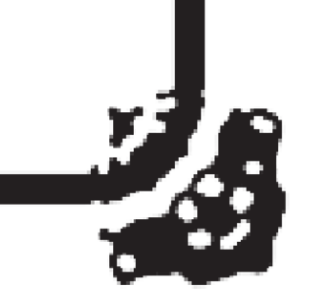
\includegraphics[width=0.4\textwidth]{image/introduction/inverse-design-bend.png}
  }

  % 2° row
  % Traditional splitter
  \subfigure[WDM con diseño tradicional]{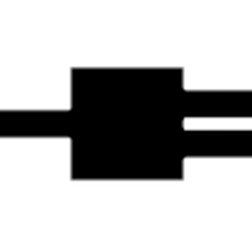
\includegraphics[width=0.4\textwidth]{image/introduction/traditional-splitter.png}}
  \hfill
  % Inverse design splitter
  \subfigure[WDM obtenido con diseño inverso. Extraído de \citep{Su2020}]{
    
\includegraphics[width=0.4\textwidth]{image/introduction/inverse-design-splitter.png}
  }

  \caption{Diseños tradicionales y obtenidos a partir de diseño inverso de un \emph{bend} y un WDM}
  \label{fig:devices}

\end{figure}


El diseño inverso ha recibido mucha atención en fotónica durante los últimos 20 años \citep{Molesky2018}. 
Los autores en \cite{Su2020} muestran estrategias para optimizar un \emph{bend} y \emph{WDM}.
En \cite{Su2018, Piggott2017} se incorporan restricciones de fabricación para obtener dispositivos que al fabricarse mantengan un buen rendimiento. 
No obstante, la búsqueda de estos diseños suele realizarse aplicando algoritmos cuya selección y configuración es mayormente debido a un tedioso proceso de prueba y error.
Otros trabajos como los de \cite{Schneider2019, Elsawy2020, Gregory2015} comparan distintos algoritmos de optimización en el diseño inverso de dispositivos fotónicos.


Aún cuando una cantidad considerable de investigaciones están usando el diseño inverso para optimizar dispositivos fotónicos, el \emph{bend} y WDM, dispositivos fundamentales para los circuitos fotónicos, aún no logran aplicación comercial \citep{Molesky2018}.
Además, existe una carencia de estudios con un enfoque computacional que intenten abordar el problema.
Asi, el objetivo de esta tesis es aplicar el conocimiento en computación para optimizar estos dispositivos y conseguir diseños que al fabricarse muestren un desempeño elevado.


\section{Descripción del Problema}


Para poder describir el funcionamiento de un dispositivo se calcula la distribución del campo eléctrico, para ello se resuelven las ecuaciones
de Maxwell \citep{Schneider2019}. 
Una forma de encontrar la solución a estas ecuaciones en cualquier geometría es utilizando un método numérico llamado diferencias finitas en el dominio de frecuencias (FDFD) \citep{Su2020}.
Con este planteamiento se selecciona una región rectangular a optimizar y se la divide  en $n \times m$  píxeles como si fuera una imagen, ver Figura \ref{fig:bend-discretization}. 
Luego, cada píxel se rellena con dos posibles materiales: óxido de silicio ($SiO_2$) o silicio ($Si$) \citep{Molesky2018}.

\begin{figure}[ht]
  \centering
  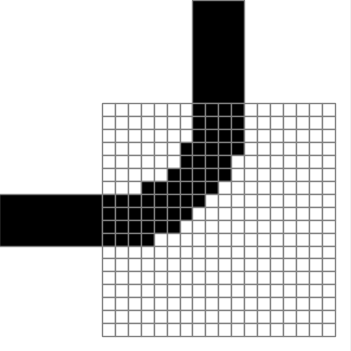
\includegraphics[scale=0.6]{image/introduction/bend-discretization.png}
  \caption{\emph{Bend} con una región de diseño discretizada en $18 \times 18$ píxeles. Cada píxel negro representa la presencia de $Si$ y cada píxel blanco de $SiO_2$}
  \label{fig:bend-discretization}
\end{figure}

El diseño inverso comienza definiendo los requerimientos del dispositivo para luego tratar de buscar entre los $2^{n \times m}$ posibles diseños algún candidato que se adapte a lo que se busca \citep{Su2020, Molesky2018}.
Como prueba de concepto, trabajos como el de \cite{Malheiros-Silveira2020} parametrizaron $2^{10 \times 10}$ posibles geometrías.
Así, se presentan algunas dificultades con esta estrategia:

\begin{enumerate}
  \item No es viable evaluar todos los posibles diseños por haber un número excesivamente elevado de ellos \citep{Vuckovic2019}.
  \item Las simulaciones computacionales son muy costosas en términos de memoria y tiempo \citep{Kudyshev2020}.
  \item El espacio de búsqueda es no convexo \citep{Su2018}.
  \item No todos los diseños son fabricables por limitaciones físicas \citep{Su2020}.
  \item Cada dispositivo es una clase distinta de problema, es decir, no necesariamente funcionará la misma estrategia para cada dispositivo \citep{Molesky2018}.
\end{enumerate}

Además, la fabricación viene con otros desafíos, principalmente:

\begin{enumerate}
  \item Errores de precisión \citep{Piggott2017}.
  \item Sensibilidad ante cambios de temperatura \citep{Vuckovic2019}.
\end{enumerate}

Considerando las anteriores dificultades, el problema es usar diseño inverso y encontrar geometrías que muestren buen desempeño en simulaciones computacionales y que puedan asegurar mantener un óptimo funcionamiento al ser fabricados. 
Este problema se estudiará para dos dispositivos nanofotónicos (i) \emph{bend} y (ii) WDM.

\section{Justificación}

El \emph{bend} y WDM son dispositivos fundamentales en los circuitos fotónicos que tienen aplicación directa, por ejemplo, en sistemas HPC \citep{Shen2017}. 
Por otro lado, desde el punto de vista computacional, este problema es interesante porque ya hay estrategias computacionales conocidas para resolverlo, desde algoritmos evolutivos \citep{Hansen2016} hasta redes neuronales \citep{Goodfellow2015} y \emph{depth learning} \citep{Malkiel2018}. 
Además, debido al alto costo computacional de las simulaciones \citep{Schneider2019}, el trabajo requiere de computación de alto desempeño.
Así, es probable que se pueda obtener buenos resultados en la investigación aplicando el conocimiento ya existente en computación. 

\section{Objetivos}

\begin{itemize}

  \item Fabricar un \emph{bend} y WDM con eficiencias mayores al noventa por ciento.

  \item Usando HPC, estudiar el desempeño y la convergencia de cinco algoritmos de optimización populares usados para optimizar dispositivos nanofotónicos.

\end{itemize}



\section{Aportes}

Este trabajo busca brindar una comparativa de las técnicas de optimización más relevantes que se aplican para optimizar un \emph{bend} y un WDM cuando estos son parametrizados con un elevado número de variables.

%\joruge{por ahora mantener, luego alinear al paper de JLT}

\chapter{Marco  Teórico}

En el presente capítulo se explican \jorge{introducen} conceptos \jorge{fundamentales} y \jorge{remover: terminología} relacionada al diseño inverso de dispositivos fotónicos.
Para ello se desarrolla tres secciones. 
En primer lugar \jorge{Primero}, se describen las propiedades físicas de interés de un \emph{bend} y WDM \jorge{corregir: consistencia en todo el texto WDM Mux o MUX}.
En segundo lugar\jorge{Segundo,} , se define \jorge{la optimización de los dispositivos estudiados en  cinco pasos (basado en CITE CITE).} sobre como utilizar el diseño inverso para optimizar los dispositivos de estudio.
  \begin{itemize}
  \item Se especifica tres estrategias comúnmente usadas para parametrizar la región de diseño.
  \item Se muestra como definir la función objetivo para un \emph{bend} y WDM.
  \item Se señala los programas donde se puede simular el comportamiento de los diseños que desarrollemos.
  \item Se expone como se explican estrategias de optimización para un dispositivo fotónico.
  \item Se da a conocer transformaciones que se pueden incluir al plan de optimización para incorporar restricciones de fabricación.
  \end{itemize}  
En tercer lugar, se explica la conversión de los resultados de la optimización a un formato listo para ser fabricado.


\section{Dispositivos de estudio}

\subsection{\emph{Bend}}

Un \emph{bend} es un dispositivo fotónico que se encarga de guiar un haz de ondas para que gire.

En general, al estudiar dispositivos fotónicos es de especial interés la distribución del campo eléctrico. 
Este campo se descompone en una componente transversal eléctrica (TE) y en una componente transversal magnética (TM) de acuerdo a la siguiente ecuación:

\begin{equation}
  E = E^{TE} + E^{TM}
\label{eq:field}
\end{equation}

Donde $E^{TE}$ es la componente paralela al dispositivo y $E^{TM}$ es la componente restante \citep{Hohenester2020}. 

La intensidad de estos campos es de especial interés pues nos dan una idea del rendimiento del dispositivo. 
Por ejemplo, en la figura \ref{fig:efield} se muestra la intensidad del campo $E^{TE}$ cuando un haz de luz está pasándo por el dispositivo. 
Como podemos observar, parte del campo está fuera del \emph{bend} representado por color morado.
Así, se visualiza de forma gráfica que el dispositivo está teniendo considerables pérdidas de energía lo cual es un indicador de un mal rendimiento.


\begin{figure}[ht]
  \centering
  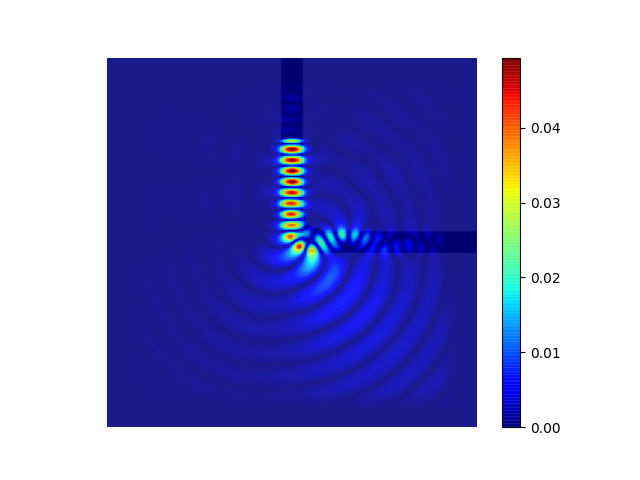
\includegraphics[scale=0.8]{image/theory/bend-field.png}
  \caption{Intensidad de campo eléctrico para un \emph{bend-90°} de radio interno de 0.25 $\mu m$}
  \label{fig:efield}
\end{figure}

Por otro lado, para evaluar el desempeño de un \emph{bend} de forma numérica se suele calcular la transmitancia como la relación entre la intensidad del haz que sale del dispositivo con la intensidad con la que entra \citep{Su2020}. Esto se expresa mediante la ecuación \ref{eq:transmission}:

\begin{equation}
  T = \frac{I}{I_0}
\label{eq:transmission}
\end{equation}


\subsection{\emph{Wavelength Demultiplexer} de dos canales (WDM)}

Un WDM es un dispositivo fotónico que se encarga de guiar un haz de ondas de acuerdo a su longitud de onda.
Así, estos suelen trabajar con dos longitudes de onda y guían las de un tipo por la guía de onda superior y las de otro tipo por la guía de onda inferior.

Similar al caso del \emph{bend} se estudia su campo eléctrico y transmitancia para medir el rendimiento de estos dispositivos.

Un dispositivo similar al WDM es un \emph{splitter}. Este dispositivo tiene la misma geometría, pero trata de dividir lo que recibe.

\section{Diseño inverso}

\subsection{Parametrización}

Tres estrategias comúnes para parametrizar un dispositivo fotónico son: i) parametrización por píxeles, ii) parametrización por conjuntos de nivel, iii) parametrización por segmentos.

\subsubsection{Parametrización basada en topología}

A cada píxel se le asocia un valor dado por la fórmula \ref{eq:permitivity} \citep{Su2020}:

\begin{equation}
  \varepsilon(x, y) = \varepsilon_{Si} + (1 - \lambda_{x,y}) \varepsilon_{SiO_2} \quad \lambda_{x, y} \in [0, 1], \lambda_{x, y} \in \mathbb{R} 
\label{eq:permitivity}
\end{equation}

Donde $\varepsilon_{Si} = 3.48$ es la permitividad del $Si$ y $\varepsilon_{SiO_2} = 1.44$ es la permitividad del $SiO2$.
Con esta ecuación se mapea el intervalo $[0, 1]$ con el intervalo $[1.44, 3.48]$. 
Esto se realiza para determinar la permitividad que hay en la ubicación del píxel y poder simular las ecuaciones de Maxwell en el dispositivo.
Con esta parametrización obtenemos una cantidad infinita de diseños, mas solo nos interesan aquellos donde $\lambda_{x,y}$ es entero, pues en caso contrario un píxel se mapea a la permitividad de un material desconocido lo cual lo volvería infabricable.


En la figura \ref{fig:pixeles} se muestra la parametrización topológica de un \emph{bend-90°}. 
Las píxeles en gris representan regiones donde se está usando una permitividad desconocida, es decir se ha tomado un $\lambda_{x,y}$ no entero.

\begin{figure}[h]
  \centering
  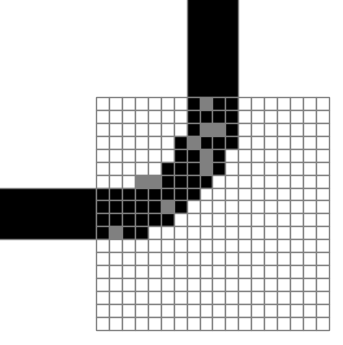
\includegraphics[scale=0.8]{image/theory/parametrization-pixeles.png}
  \caption{Parametrización por píxeles para un \emph{bend-90°}}
  \label{fig:pixeles}
\end{figure}


\subsubsection{Parametrización por conjuntos de nivel}

A cada píxel se le asocia una permitividad dada por la siguiente fórmula \citep{Piggott2017}:

  \[ \varepsilon(x, y) =
    \begin{cases}
      \varepsilon_{Si}       & \quad \text{si } \phi(x, y) \leq 0\\
      \varepsilon_{SiO_2}    & \quad \text{si } \phi(x, y) > 0
    \end{cases}
  \]

Donde $\phi$ se define como una función contínua. 
En la figura \ref{fig:levelsets} se muestra como esta parametrización permite mantener curvas continuas para representar al dispositivo (líneas amarillas).
Luego, los píxeles intentan cubrir la región definida por estas curvas para después poder simular numéricamente las propiedades del dispositivo.

\begin{figure}[h]
  \centering
  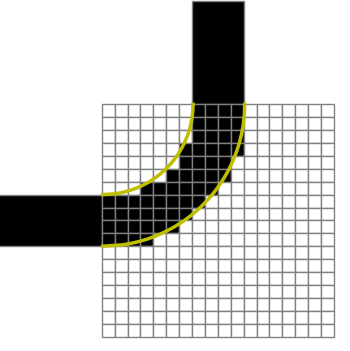
\includegraphics[scale=0.8]{image/theory/parametrization-levelsets.png}
  \caption{Parametrización por conjuntos de nivel para un \emph{bend-90°}}
  \label{fig:levelsets}
\end{figure}




\subsubsection{Parametrización por segmentos}

Con esta estrategia se considera la región de diseño como un rectángulo y se lo divide en $n$ segmentos de igual tamaño. 
Luego, el tamaño de cada segmento será un parámetro y la geometría se forma a partir de estos valores considerando ubicar cada segmento centrado verticalmente. 
%En la figura \ref{fig:splines} podemos observar como \cite{Prosopio-Galarza2019} utiliza esta parametrización con $13$ segmentos para diseñar un 2-splitter.


%\begin{figure}[ht]
%  \centering
%  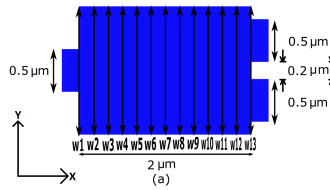
\includegraphics[scale=0.8]{image/theory/parametrization-spline.png}
%  \caption{Parametrización por 13 segmentos de un \emph{2-splitter}. Imagen extraída de \cite{Prosopio-Galarza2019}}
%  \label{fig:splines}
%\end{figure}


Las distintas estrategias de parametrización mostradas tienen sus propias características.
La parametrización por segmentos asegura simetría y regiones compactas, pero tiene un espacio de búsqueda más reducido que las otras opciones.
Por otro lado, la parametrización topológica trabaja con un espacio de búsqueda mucho más grande a cambio de poder parametrizar diseños no fabricables.
En cambio, la parametrización por niveles se encarga de mantener una curva continua con el fin de mantener el diseño similar a como terminará el dispositivo fabricado.

\subsection{Definición de la función objetivo}

La función objetivo es un valor asociado a una parametrización que nos permite comparar distintas parametrizaciones para determinar que diseño es mejor. 
En el área de fotónica es común referirse a esta función como la figura de mérito (FOM). 
Basándonos en \cite{Su2020} se tiene que conviene definir la FOM de la siguiente manera:

\begin{enumerate}

\item \emph{Bend}

\begin{equation}
  f_{obj}(p) = max \left \{ T(p) \right \}
\label{eq:fom-bend}
\end{equation}

Es decir, la función objetivo asociada a la parametrización $p$ es maximizar la transmitancia, ver equación \ref{eq:transmission}, asociada a esa parametrización.

\item WDM

La función objetivo se define como:

\begin{equation}
  f_{obj}(p) = max \left \{ g_0(p, 0)^2 + (1 - g_0(p, 1))^2 + g_1(p, 1)^2 + (1 - g_1(p, 0))^2 \right \}
\label{eq:fom-splitter}
\end{equation}

Donde $g_0(p, i)$ representa la transmitancia asociada a la parametrización $p$ en la guía de onda $i$ para una longitud de onda de $1400 nm$ y 
      $g_1(p, i)$ representa su análogo para una longitud de onda de $1550 nm$.

La ecuación \ref{eq:fom-splitter} busca maximizar la transmitancia por la guía de onda superior y minimizarla para la guía de onda inferior cuando se recibe una longitud de onda de $1400 nm$ y lo contrario para una longitud de onda de $1550 nm$.

\end{enumerate}

\subsection{Simulación}

Existen distintas librerías de Python que nos permiten definir dispositivos fotónicos en base a lo descrito. 
Dos librerías muy usadas para ello son MEEP \citep{Oskooi2010} y SPINS \citep{Su2020}. 
Una evaluación cualitativa de sus funcionalidades puede ser vista en la tabla \ref{tab:simulation}.

\begin{table}[ht]
    \centering
    \begin{tabular}{|c|c|c|c|c|}
    \hline 
    Librería &  Usabilidad & Eficiencia & Bugs & Funcionalidad \\
    \hline 
    MEEP &  Difícil & Alta & Elevados & Extensa \\
    SPIN &  Moderada  & Moderada-Alta & Pocos & Básica necesaria \\
    \hline 
    \end{tabular}
    \caption{Evaluación cualitativa de las librerías MEEP y SPINS}
    \label{tab:simulation}
\end{table}


Ambas librerías se encargan de realizar la simulación en una región cuadrada, para ello dividan la región de simulación como si fuera una cuadrícula.
Definiendo la resolución podemos especificar el tamaño de esta cuadrícula. 
Entre más pequeña sean las divisiones de esta, más cercanos a los valores reales sean los resultados de la simulación.
Sin embargo, esto implica un mayor tiempo de ejecución.


\subsection{Estrategias de optimización}

La forma de optimizar un diseño depende de la parametrización utilizada. De esta forma, tenemos los siguientes casos:

\begin{enumerate}


\item{Parametrización topológica}


La ecuación \ref{eq:permitivity} ya señala un rango de valores asociados a cada píxel. 
Pero, para asegurar el obtener un diseño fabricable se divide la optimización en dos pasos \citep{Su2020}:

  \begin{enumerate}
  \item Optimización continua
  
  Se varía el valor de $\lambda_{x,y}$ en el intervalo $[0, 1]$ sin importar si se obtiene diseños no fabricables.

  \item Optimización discreta

  Se considera el resultado de la optimización continua como punto inicial del algoritmo de optimización.
  Luego, se va aplicando una transformación que permita ir convergencia a una parametrización donde cada $\lambda_{x, y}$ tenga un valor entero.
  Algunos ejemplos de estas transformaciones se pueden encontrar en la siguiente sección.

  \end{enumerate}

\item{Parametrización por conjuntos de nivel}

Como lo detalla \cite{Piggott2017}, con este tipo de parametrización es conveniente utilizar una optimización basada en la gradiente y
asegurar convergencia con una búsqueda en línea.

\item{Parametrización por segmentos}

Basándonos en \cite{Prosopio-Galarza2019}, con este tipo de parametrización conviene definir un rango de posibles valores para cada segmento.
Luego, ejecutar algún algoritmo de optimización, de preferencia uno de optimización global, para finalmente tratar de incorporar restricciones de fabricación en una etapa posterior.

\end{enumerate}

\subsection{Transformaciones}

La aplicación de transformaciones a un diseño se realiza con el fin de obtener dispositivos con curvas suaves para asegurar un buen desempeño al momento de fabricarse \citep{Su2020}. 
De acuerdo al tipo de parametrización utilizada, tenemos:

\begin{itemize}
  \item Para el caso de la parametrización por segmentos, si queremos suavizar el diseño obtenido podemos considerar las alturas de los segmentos e interpolar una curva \citep{Yangjin2013}.

  \item Para el caso de la parametrización por conjunto de nivel se define $\phi$ de forma que asegure curvas suaves, así no es necesario aplicar transformaciones.

  \item Para el caso de la parametrización topológica, una forma se suavizar las regiones punteagudas es aplicar una función de suavizado conforme va iterando el algoritmo de optimización aplicado. Basándonos en \cite{Zhang2021}, podemos aplicar la siguiente función:

\begin{equation}
  s(p) = \frac{\tanh (\beta \times \eta) + \tanh (\beta \times (p - \eta))}{\tanh (\beta \times \eta) + \tanh (\beta \times (1 - \eta))}
  \label{eq:topo-smooth}
\end{equation}

    Donde $p$ es la parametrización del dispositivo, $\eta = 0.5$ y $\beta$ comienza con un valor de 1 y va incrementándose exponencialmente en cada iteración. 
    Como se observa en la figura \ref{fig:discretization}, la ecuación \ref{eq:topo-smooth} se encarga de ir haciendo converger los valores de la parametrización a $0$ o $1$ de acuerdo a cual esté más cercano. 
    Conforme aumenta el valor de $\beta$ esta convergencia es más rápida.

    \begin{figure}[ht]
      \centering
      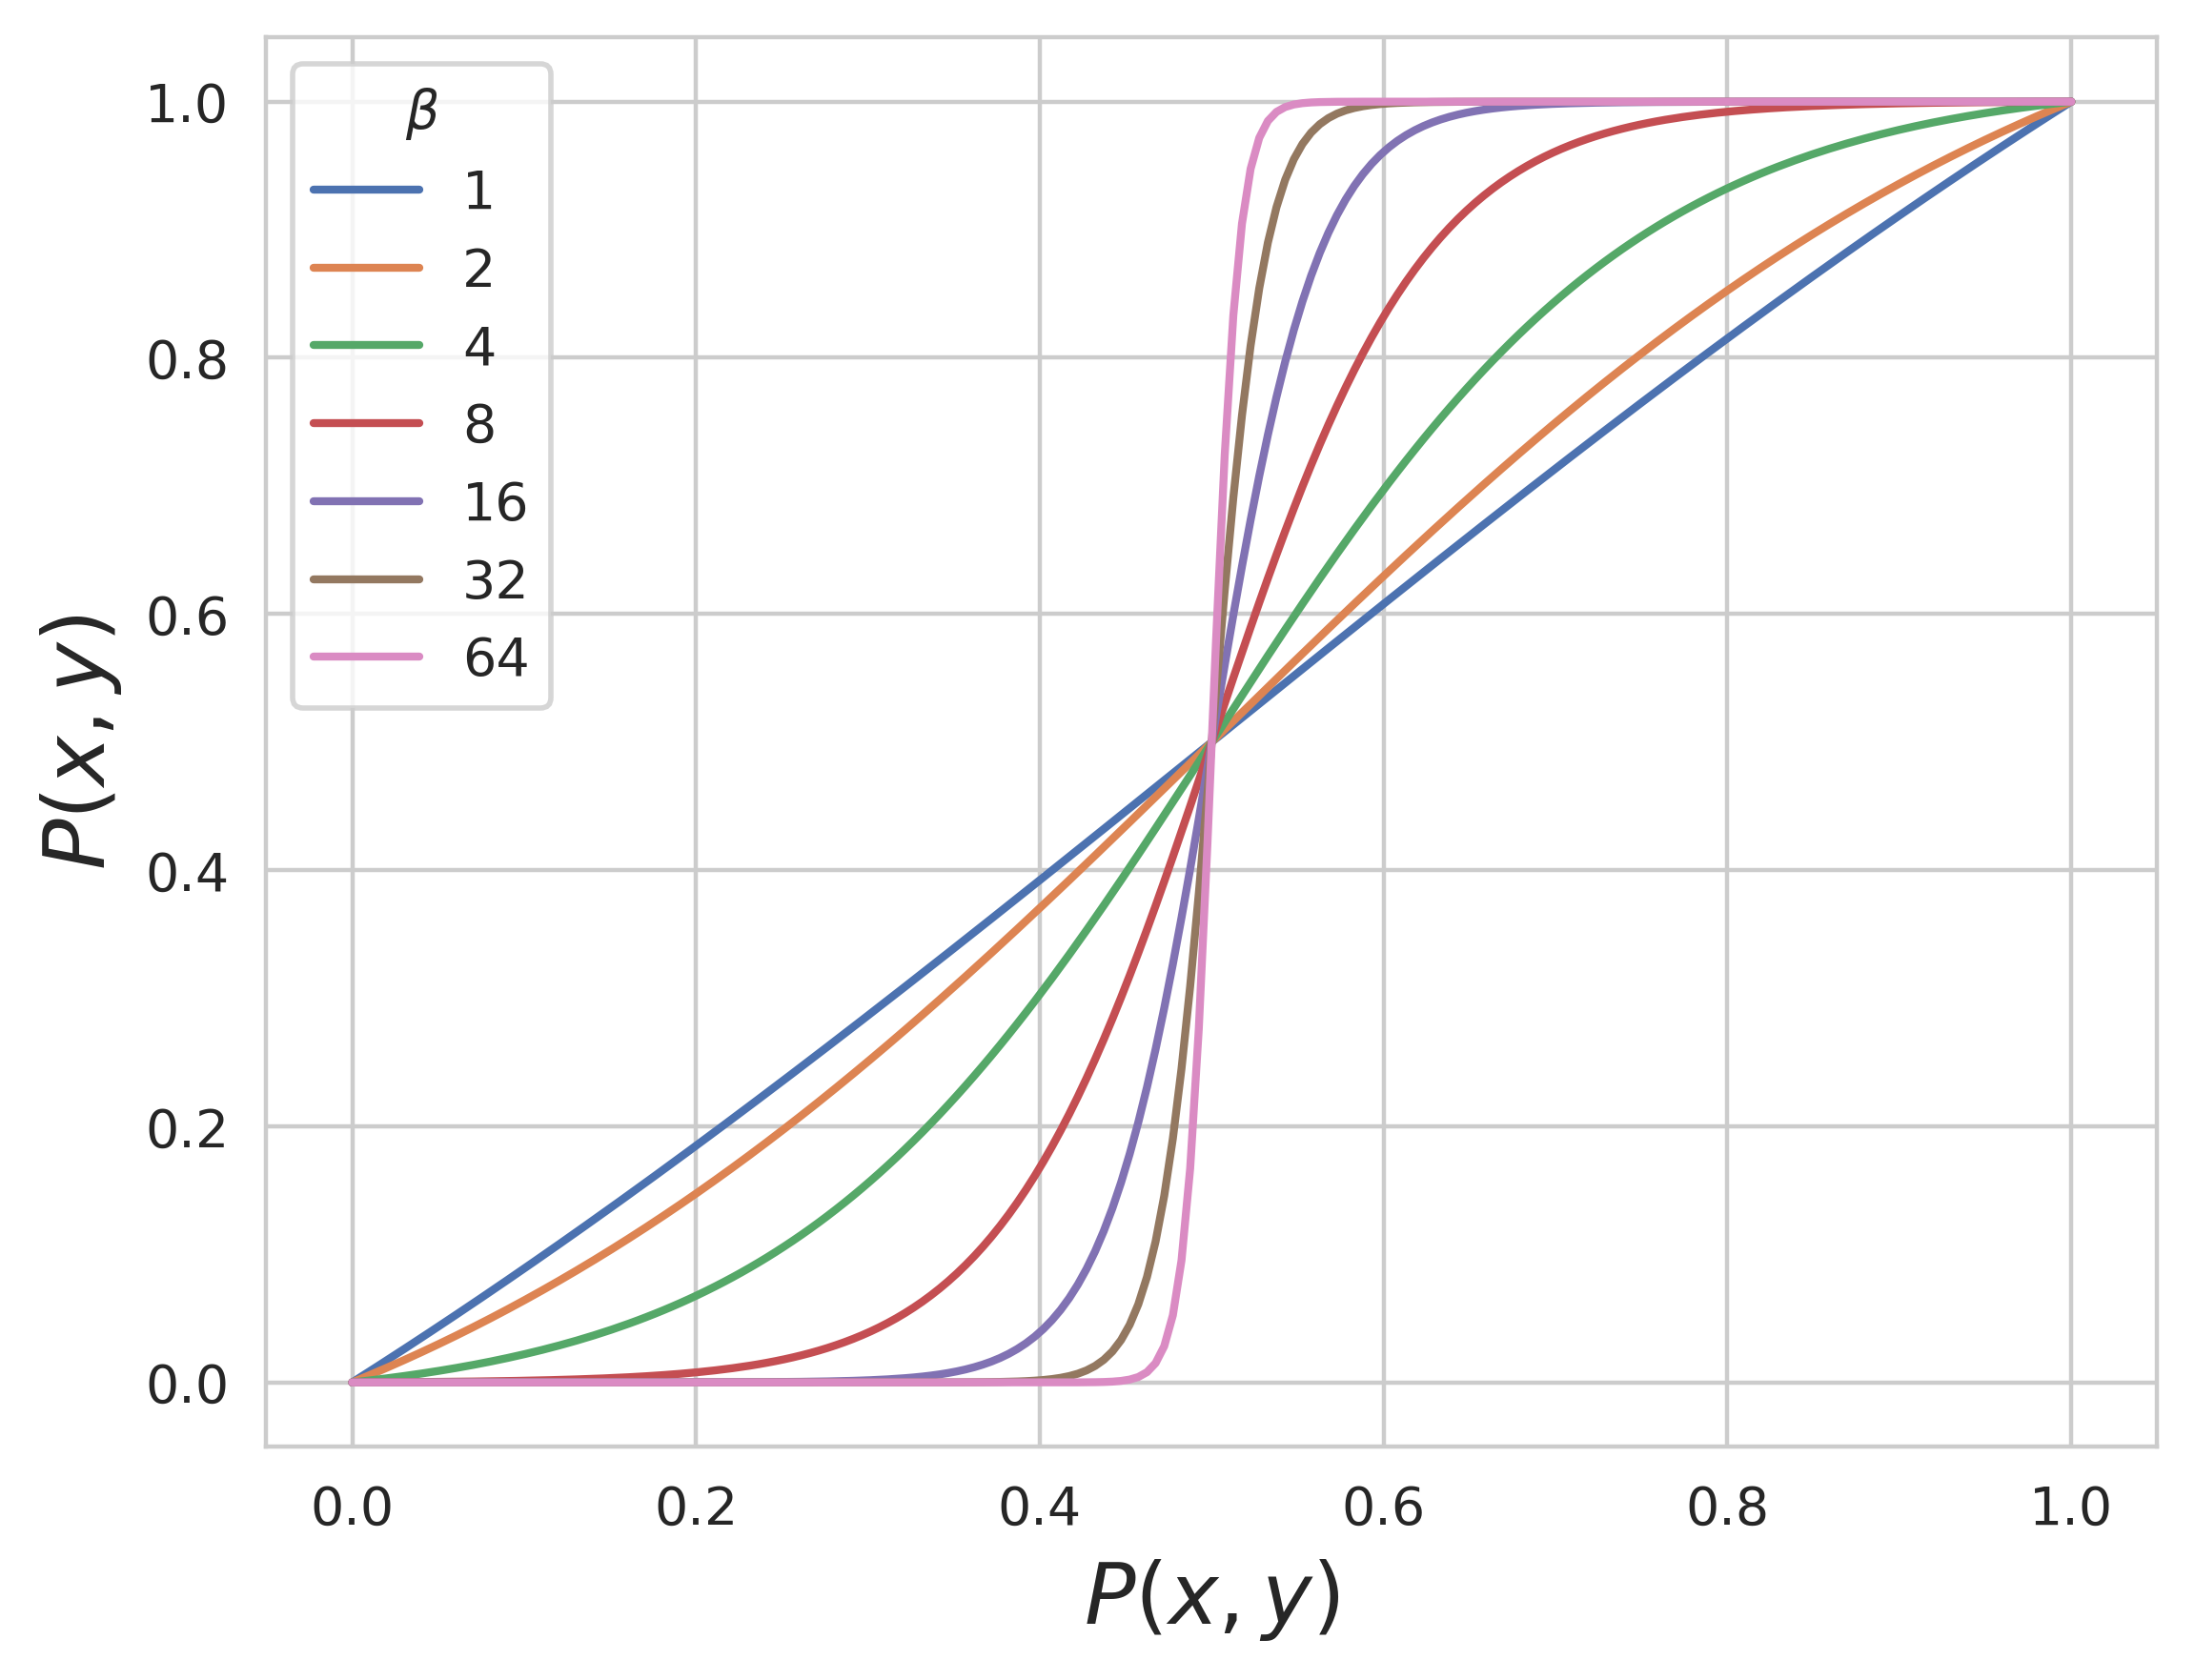
\includegraphics[scale=0.8]{image/theory/discretization.png}
      \caption{Función de discretización con $\eta = 0.5$ y distintos valores de $\beta$}
      \label{fig:discretization}
    \end{figure}

\end{itemize}

\section{Preparación para fabricación}

Para poder fabricar nuestros diseños necesitamos representarlos en formato GDSII.
En este formato se especifica los polígonos que representan a nuestro dispositivo.
Independientemente de la parametrización utilizada, mediante la simulación con SPINS o MEEP se puede obtener los puntos asociados al contorno del dispositivo.
Así, utilizando lo anterior se construye los polígonos \citep{Bogaerts2018}.

\chapter{Trabajos relacionados}

Usted deberá buscar, revisar, seleccionar y estudiar un conjunto de artículos  pertenecientes  al  estado del arte  y  que además, sean relevantes en su área de investigación. (Entre 2 a 3 páginas)\\


La sección de trabajo relacionados, deberá contener un resumen, claro y conciso, de aquellos trabajos de investigación que están directamente relacionados con vuestro trabajo. Esto con el objetivo que el lector pueda darse cuenta de las diferencias entre su propuesta y las del estado del arte, además, permitirá saber como otros autores han intentado resolver un problema similar al suyo.


\chapter{Metodología}\label{chapter:methodology}

En el presente capítulo se describe la metodología a seguir en esta tesis.
Primero, se describe de forma general los seis pasos que se trabajaran.
Luego, se detalla en una sección completa cada uno de estos.
Finalmente, se brindan los alcances y limitaciones de la propuesta.

Como se muestra en la \autoref{fig:pipeline}, en esta investigación se siguieron los siguientes seis pasos:
(i) preparación de simulación, 
(ii) preparación de optimización, 
(iii) optimización continua,
(iv) optimización discreta,
(v) optimización de fabricación y
(vi) preparación para fabricación.

Estos pasos se siguieron para optimizar tanto un \emph{bend} como un WDM.
Una vez preparada la simulación, la etapa de optimización (continua, discreta y de fabricación) se realizó
tres veces por cada algoritmo.
La primera ejecución usa un valor de semilla de 128, la segunda de 256 y la tercera de 512.
De esta manera se aseguró iniciar con diseños aleatorios y mantener los resultados reproducibles.

Es importante señalar que los resultados de la optimización continua se usan como punto de inicio
para la optimización discreta. Asimismo, los resultados de la optimización discreta se utilizan como
entrada para la optimización de fabricación.
Este proceso tiene como fin el mantener un buen resultado \citep{Yang2017}.


En particular, el valor de $\beta$, presente en la \autoref{eq:projection}, representa el factor discretizador de nuestros diseños.
Este valor se va incrementando en la optimización discreta y de fabricación como se muestra en la
\autoref{fig:pipeline}.
Finalmente, tras haber conseguido diseños optimizados se realizó un posprocesamiento y
análisis de los diseños más óptimos.

En las siguientes subsecciones se explica en detalle cada una de los pasos de la metodología seguida en esta tesis.

\begin{figure}[ht]
  \centering
  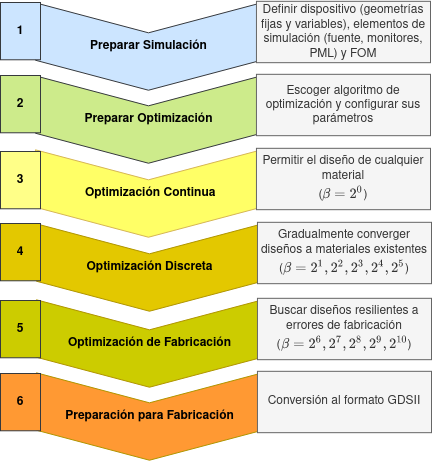
\includegraphics[scale=0.8]{image/proposal/pipeline.png}
  \caption{Metodología del trabajo de investigación}
  \label{fig:pipeline}
\end{figure}

\section{Preparación de Simulación}\label{sec:preparar-simulacion}

El \emph{bend} y WDM se parametrizaron usando la parametrización basada en píxeles descrita en la
\autoref{sec:parametrization}.
La implementación se realizó en SPINS.
La descripción detallada para los dos dispositivos de estudio se presentan en las siguientes dos subsecciones.

\subsection{\emph{Bend}}

\begin{figure}[ht]
  \centering
  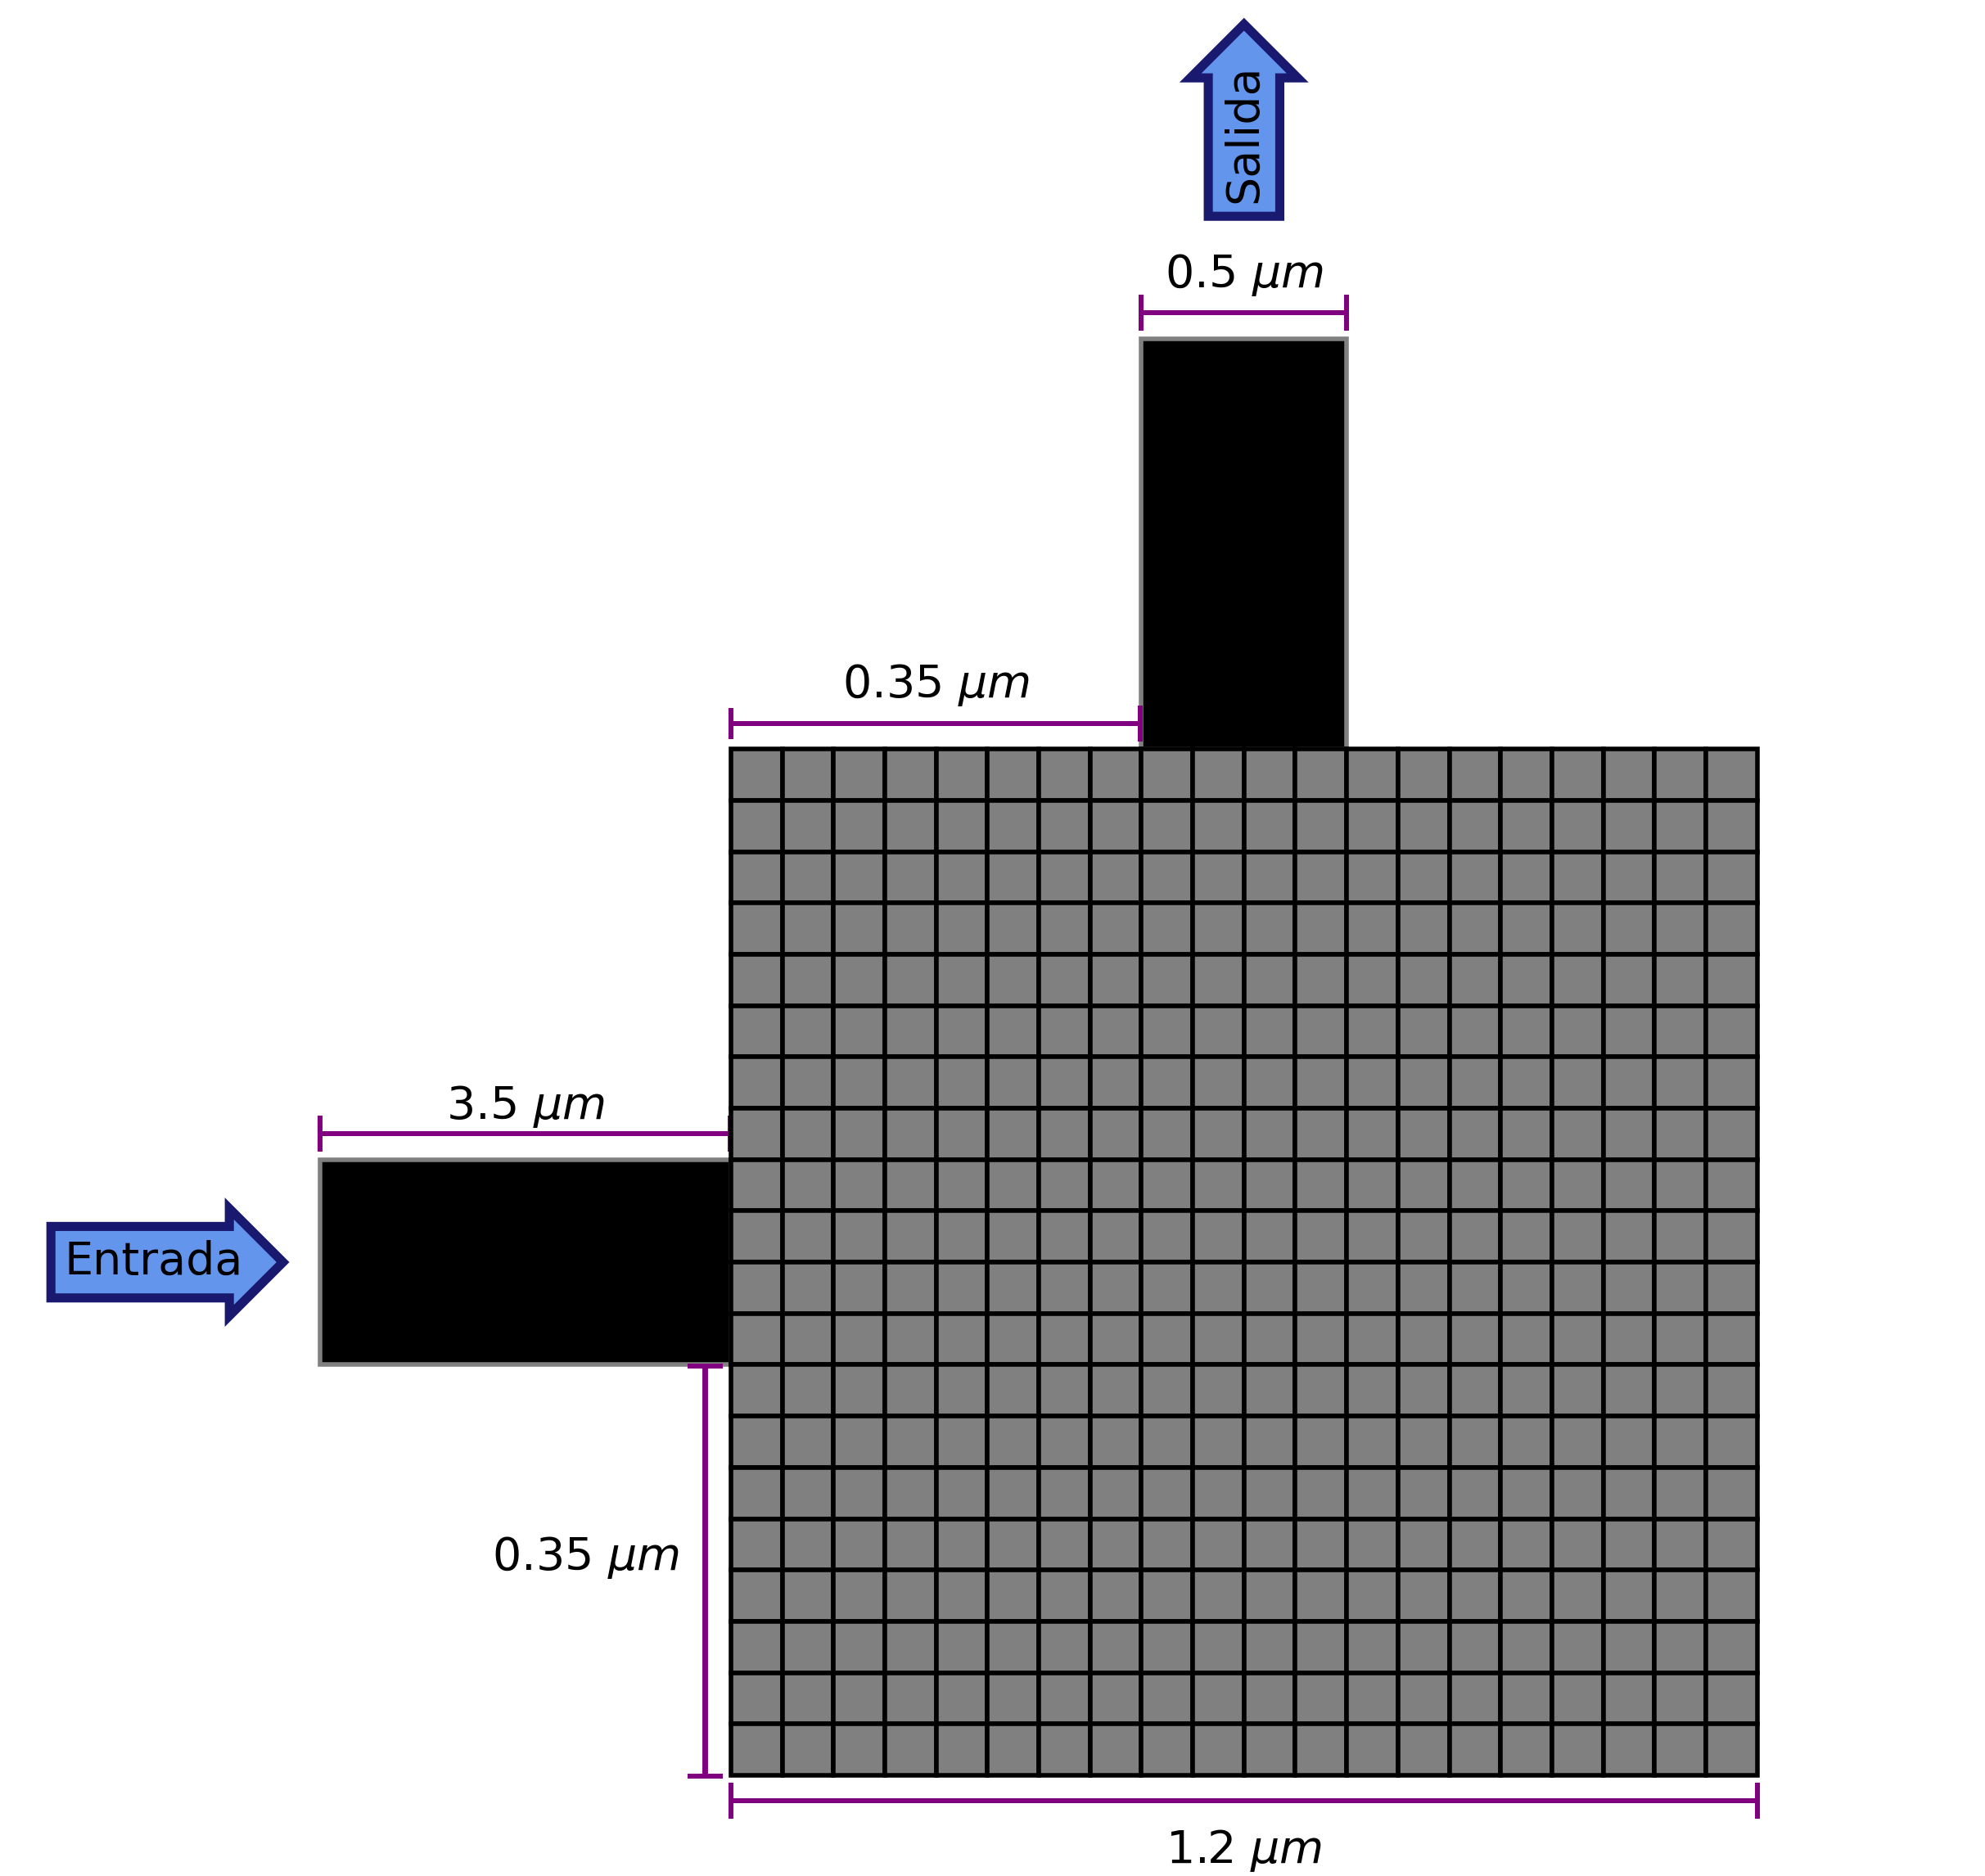
\includegraphics[width=0.6\textwidth]{image/proposal/bend.png}
  \caption{Parámetros del diseño del \emph{bend} a optimizar.}
  \label{fig:dimensiones-bend}
\end{figure}

En la \autoref{fig:dimensiones-bend} se muestra el diseño y parámetros del \emph{bend} a utilizar.
Se espera que este dispositivo trabaje a $1550 nm$.
Los rectángulo negros representan las guías de onda, estos tienen las mismas dimensiones aunque en distinta orientación.
La región gris representa la región de diseño.
La recta roja simula la fuente y la recta azul el monitor, su extensión está
simbolizada por las variables \emph{source} y \emph{monitor}, respectivamente.
Además, la profundidad de estos dos elementos es la misma, valor denotado como \emph{z\_length}.
Por otro lado, la región punteada se utiliza como referencia para definir el PML (región verde),
del cual dista un valor definido como \emph{pml\_dist}. 
La profundidad de toda la geometría es especificada por la variable \emph{depth}.

Cabe destacar que los parámetros fueron escogidos inspirados por el trabajo de \cite{Su2020}.
De este modo, la región de diseño se dividió en rectángulos de $16nm \times 16 nm$, obteniendo así una
matriz de $125 \times 125$.
Notemos que con esta configuración, en la \autoref{eq:distance} tenemos $psize_x = psize_y = 16 nm$.
El valor de los demás parámetros del diseño se presenta en la \autoref{tab:bend-values}.

\begin{table}[ht]
    \centering
    \begin{tabular}{|c|c|}
    \hline 
    Parámetro &  Valor (nm) \\
    \hline 
    wg\_height & 400 \\
    pml & 300 \\
    pml\_dist & 200 \\
    $d_1$ & 400 \\
    $d_2$ & 400 \\
    L\_width & 2000 \\
    L\_height & 2000 \\
    source & 2500 \\
    monitor & 2500 \\
    z\_length & 1000 \\
    depth & 220 \\
    \hline 
    \end{tabular}
    \caption{Parámetros usados en el diseño del \emph{bend} a optimizar.}
    \label{tab:bend-values}
\end{table}

\subsection{WDM}

\begin{figure}[ht]
  \centering
  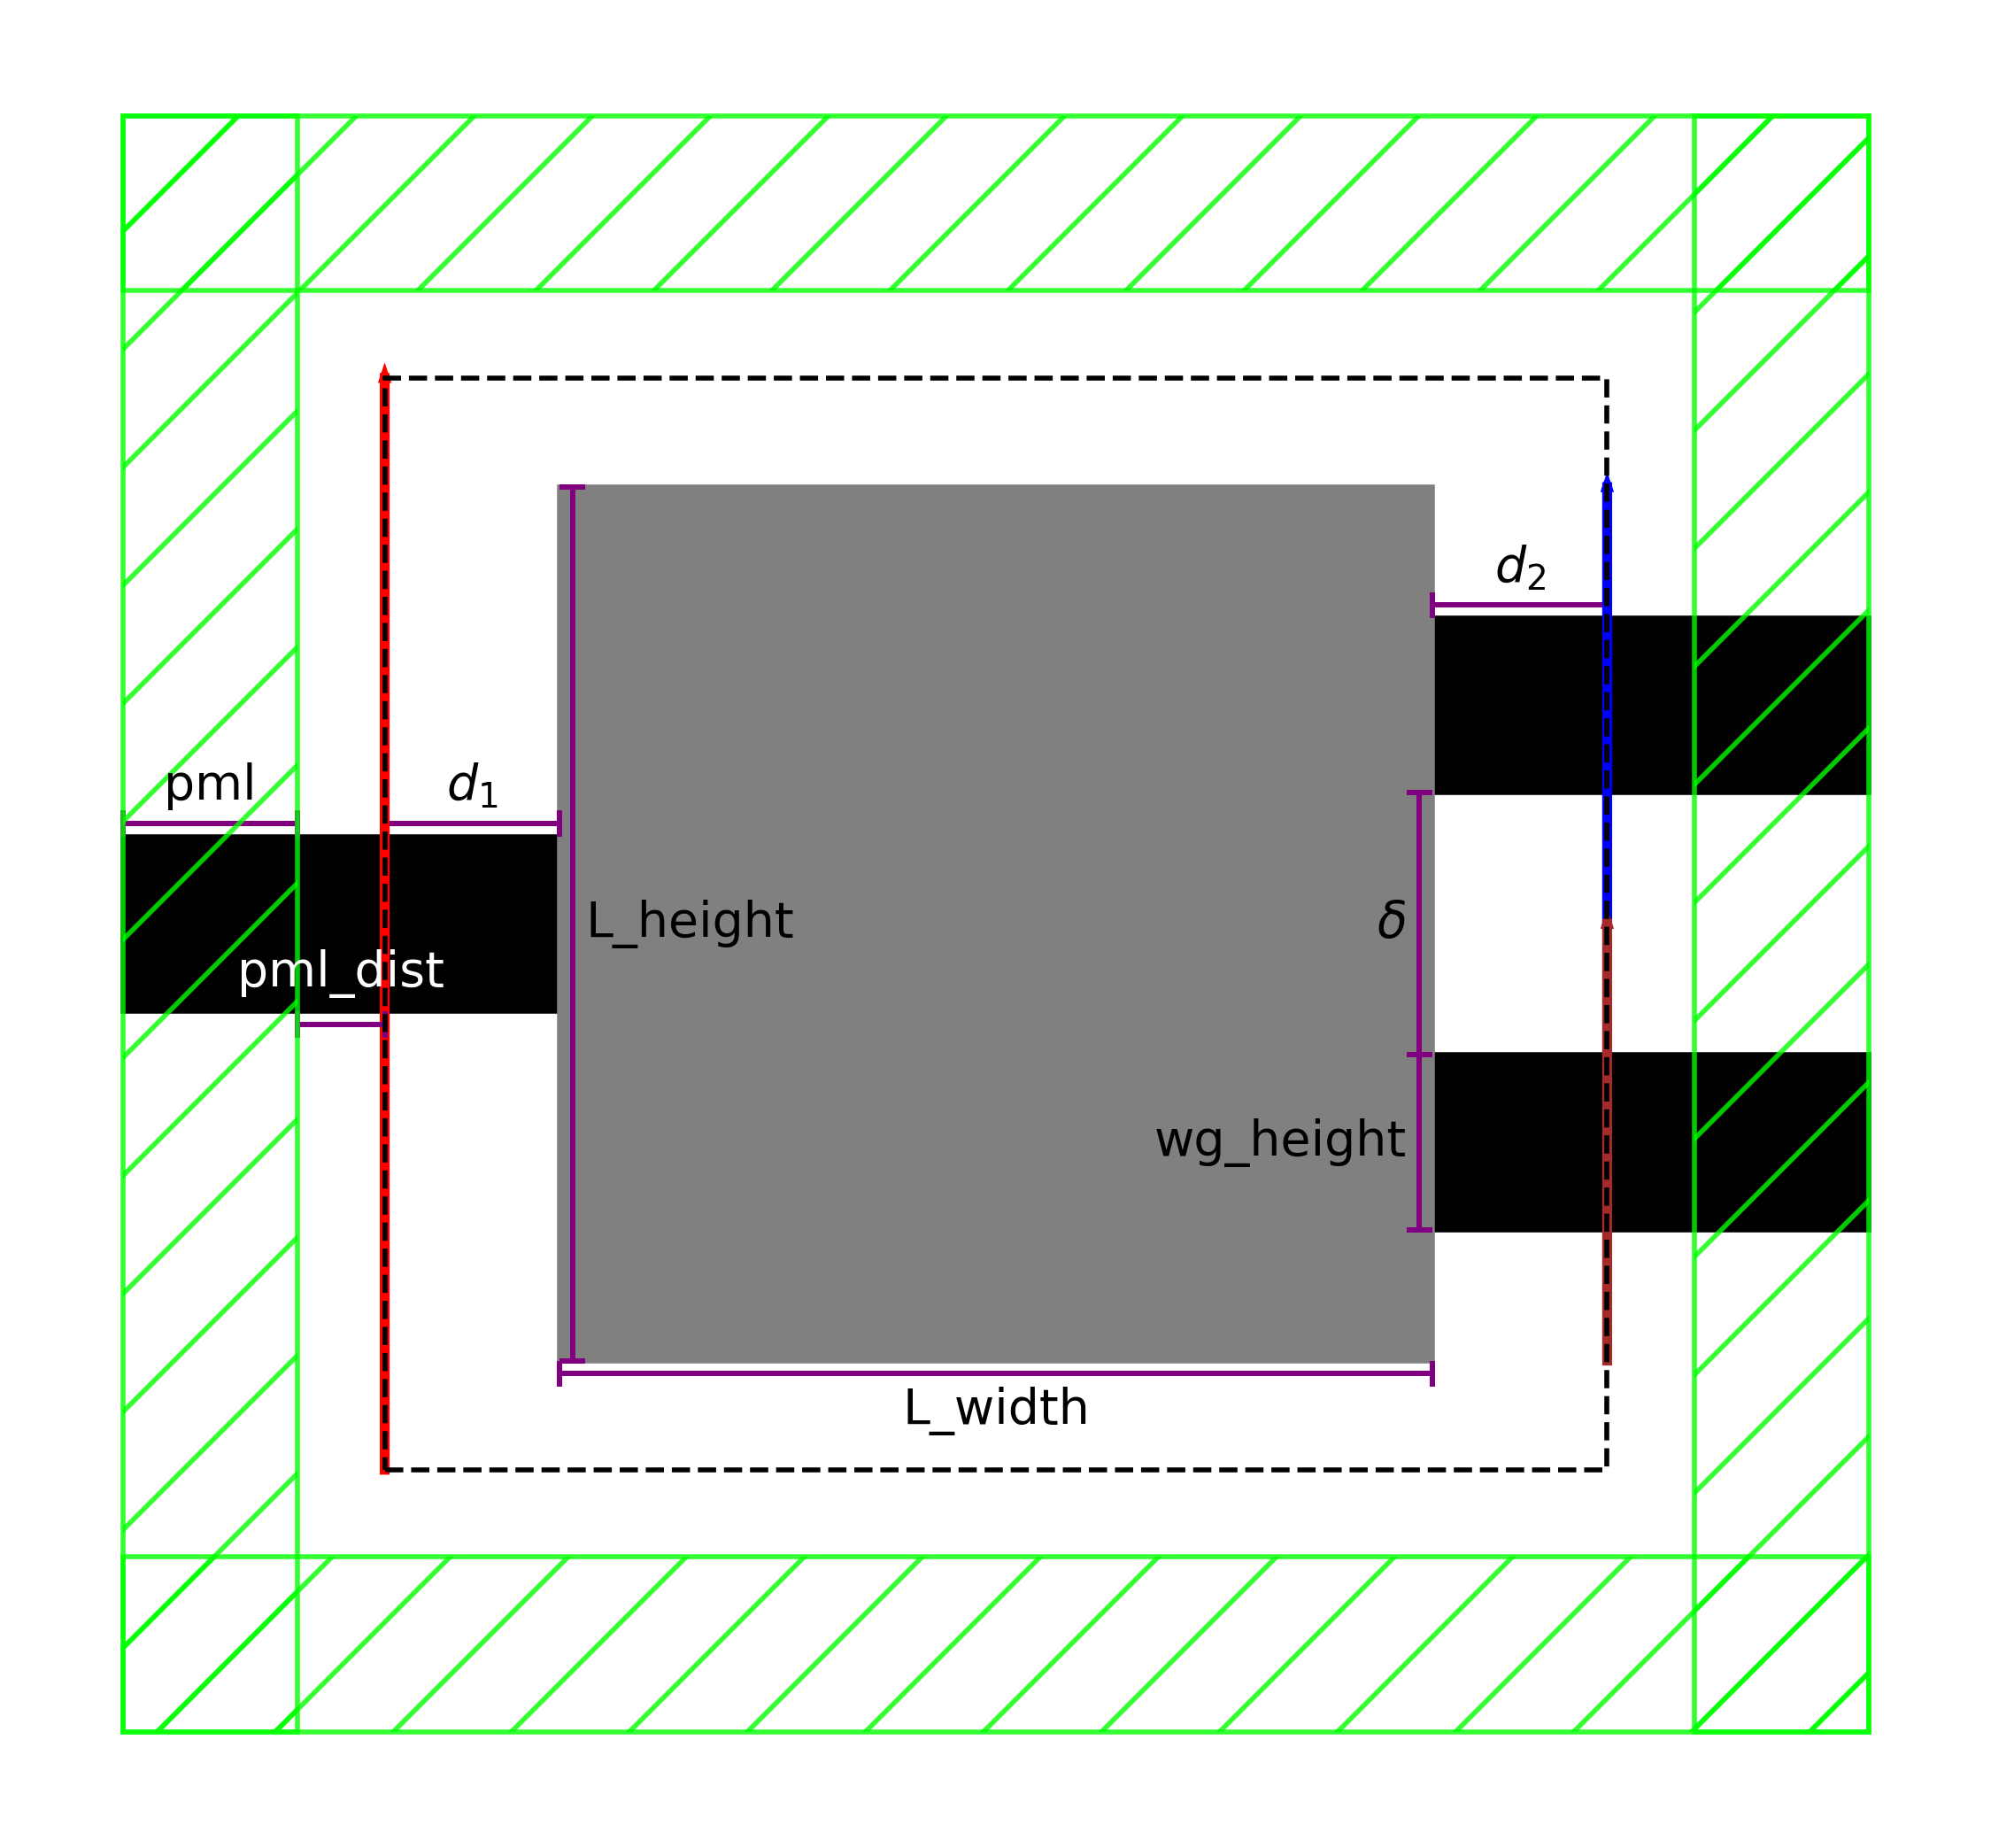
\includegraphics[width=0.6\textwidth]{image/proposal/wdm.png}
  \caption{Parámetros del diseño del WDM a optimizar.}
  \label{fig:dimensiones-demultiplexer}
\end{figure}

En la \autoref{fig:dimensiones-demultiplexer} se muestra el diseño y parámetros del WDM a utilizar.
Se espera que este dispositivo trabaje a $1300 nm$ en el brazo superior y a $1550 nm$ en el brazo inferior.
Los rectángulo negros representan las guías de onda, estos tienen las mismas dimensiones.
La región gris representa la región de diseño.
La recta roja simula la fuente y su extensión se simboliza por la variable \emph{source}.
Las rectas azul y marrón describen los monitores cuya extensión está definida por las variables \emph{monitor}.
Además, la profundidad de la fuente y monitores es la misma, denotado como \emph{z\_length}.
Por otro lado, la región punteada se utiliza como referencia para definir el PML (región verde),
del cual dista un valor definido como \emph{pml\_dist}.
La profundidad de toda la geometría es especificada por la variable \emph{depth}.

En este caso, los parámetros fueron escogidos inspirados por el trabajo de \cite{Christiansen2021}.
Del mismo modo como se realizó para el \emph{bend}, 
la región de diseño se dividió en rectángulos de $16nm \times 16 nm$, obteniendo así una
matriz de $125 \times 125$.
El valor de los demás parámetros se presenta en la \autoref{tab:wdm-values}.

\begin{table}[ht]
    \centering
    \begin{tabular}{|c|c|}
    \hline 
    Parámetro &  Valor (nm) \\
    \hline 
    wg\_height & 400 \\
    pml & 300 \\
    pml\_dist & 200 \\
    $d_1$ & 400 \\
    $d_2$ & 400 \\
    L\_width & 2000 \\
    L\_height & 2000 \\
    $\delta$ & 600 \\
    source & 2500 \\
    monitor & 1000 \\
    z\_length & 1000 \\
    depth & 220 \\
    \hline 
    \end{tabular}
    \caption{Parámetros usados en el diseño del WDM a optimizar.}
    \label{tab:wdm-values}
\end{table}


\section{Preparación de Optimización}

Con lo descrito en la anterior sección ya podemos evaluar distintos diseños.
Ahora, utilizando como función objetivo la \autoref{eq:fom-bend} para el \emph{bend} y 
la \autoref{eq:fom-splitter} para el WDM,
estamos ante un problema de optimización.
Para resolverlo, la propuesta inicial era utilizar estos cinco algoritmos:
(i) GA, (ii) PSO, (iii) CMA-ES, (iv) L-BFGS-B, (v) MMA.

La elección de estos fue por diversos motivos.
GA y PSO se escogieron por ser populares en el área \citep{Elsawy2020, Molesky2018, Prosopio-Galarza2019}.
CMA-ES por haber tenido un buen desempeño en \cite{Gregory2015} y las buenas referencias brindadas en
\cite{Campbell2019}.
L-BFGS-B por haber obtenido buenos resultados en trabajos como \cite{Su2020}.
MMA por haber sido recomendado como un buen candidato para la optimización topológica \citep{Christiansen2021}.

Por trabajos como los de \cite{Su2020} y \cite{Christiansen2021} ya nos podíamos anticipar que al usar
L-BFGS-B o MMA se obtendrían buenos resultados en parte gracias a usar la gradiente para guiar la búsqueda.
Sin embargo, por la cantidad de variables utilizadas ($125 \times 125$) no podíamos asegurar lo mismo
con GA, PSO y CMA. 

Debido a ello, primero se realizó un experimento preliminar para evaluar el desempeño de estos
algoritmos al realizar como máximo 1200 evaluaciones en la optimización del \emph{bend} propuesto, 
estos resultados son presentados en la \autoref{fig:gradient-free-comparison}.
Como podemos observar, especialmente del CMA-ES, hay una ligera tendencia de mejora.
Por otro lado, por los resultados mostrados en \cite{Christiansen2021matlab} uno esperaría que algoritmos como GA lograran 
obtener resultados similares a los obtenidos por algún algoritmo basado en la gradiente (e.g. L-BFGS-B y MMA); 
sin embargo, esto podría necesitar evaluar el FOM un número muy elevado de veces (entre $10^4$ y $10^5$).

\begin{figure}[ht]
  \centering
  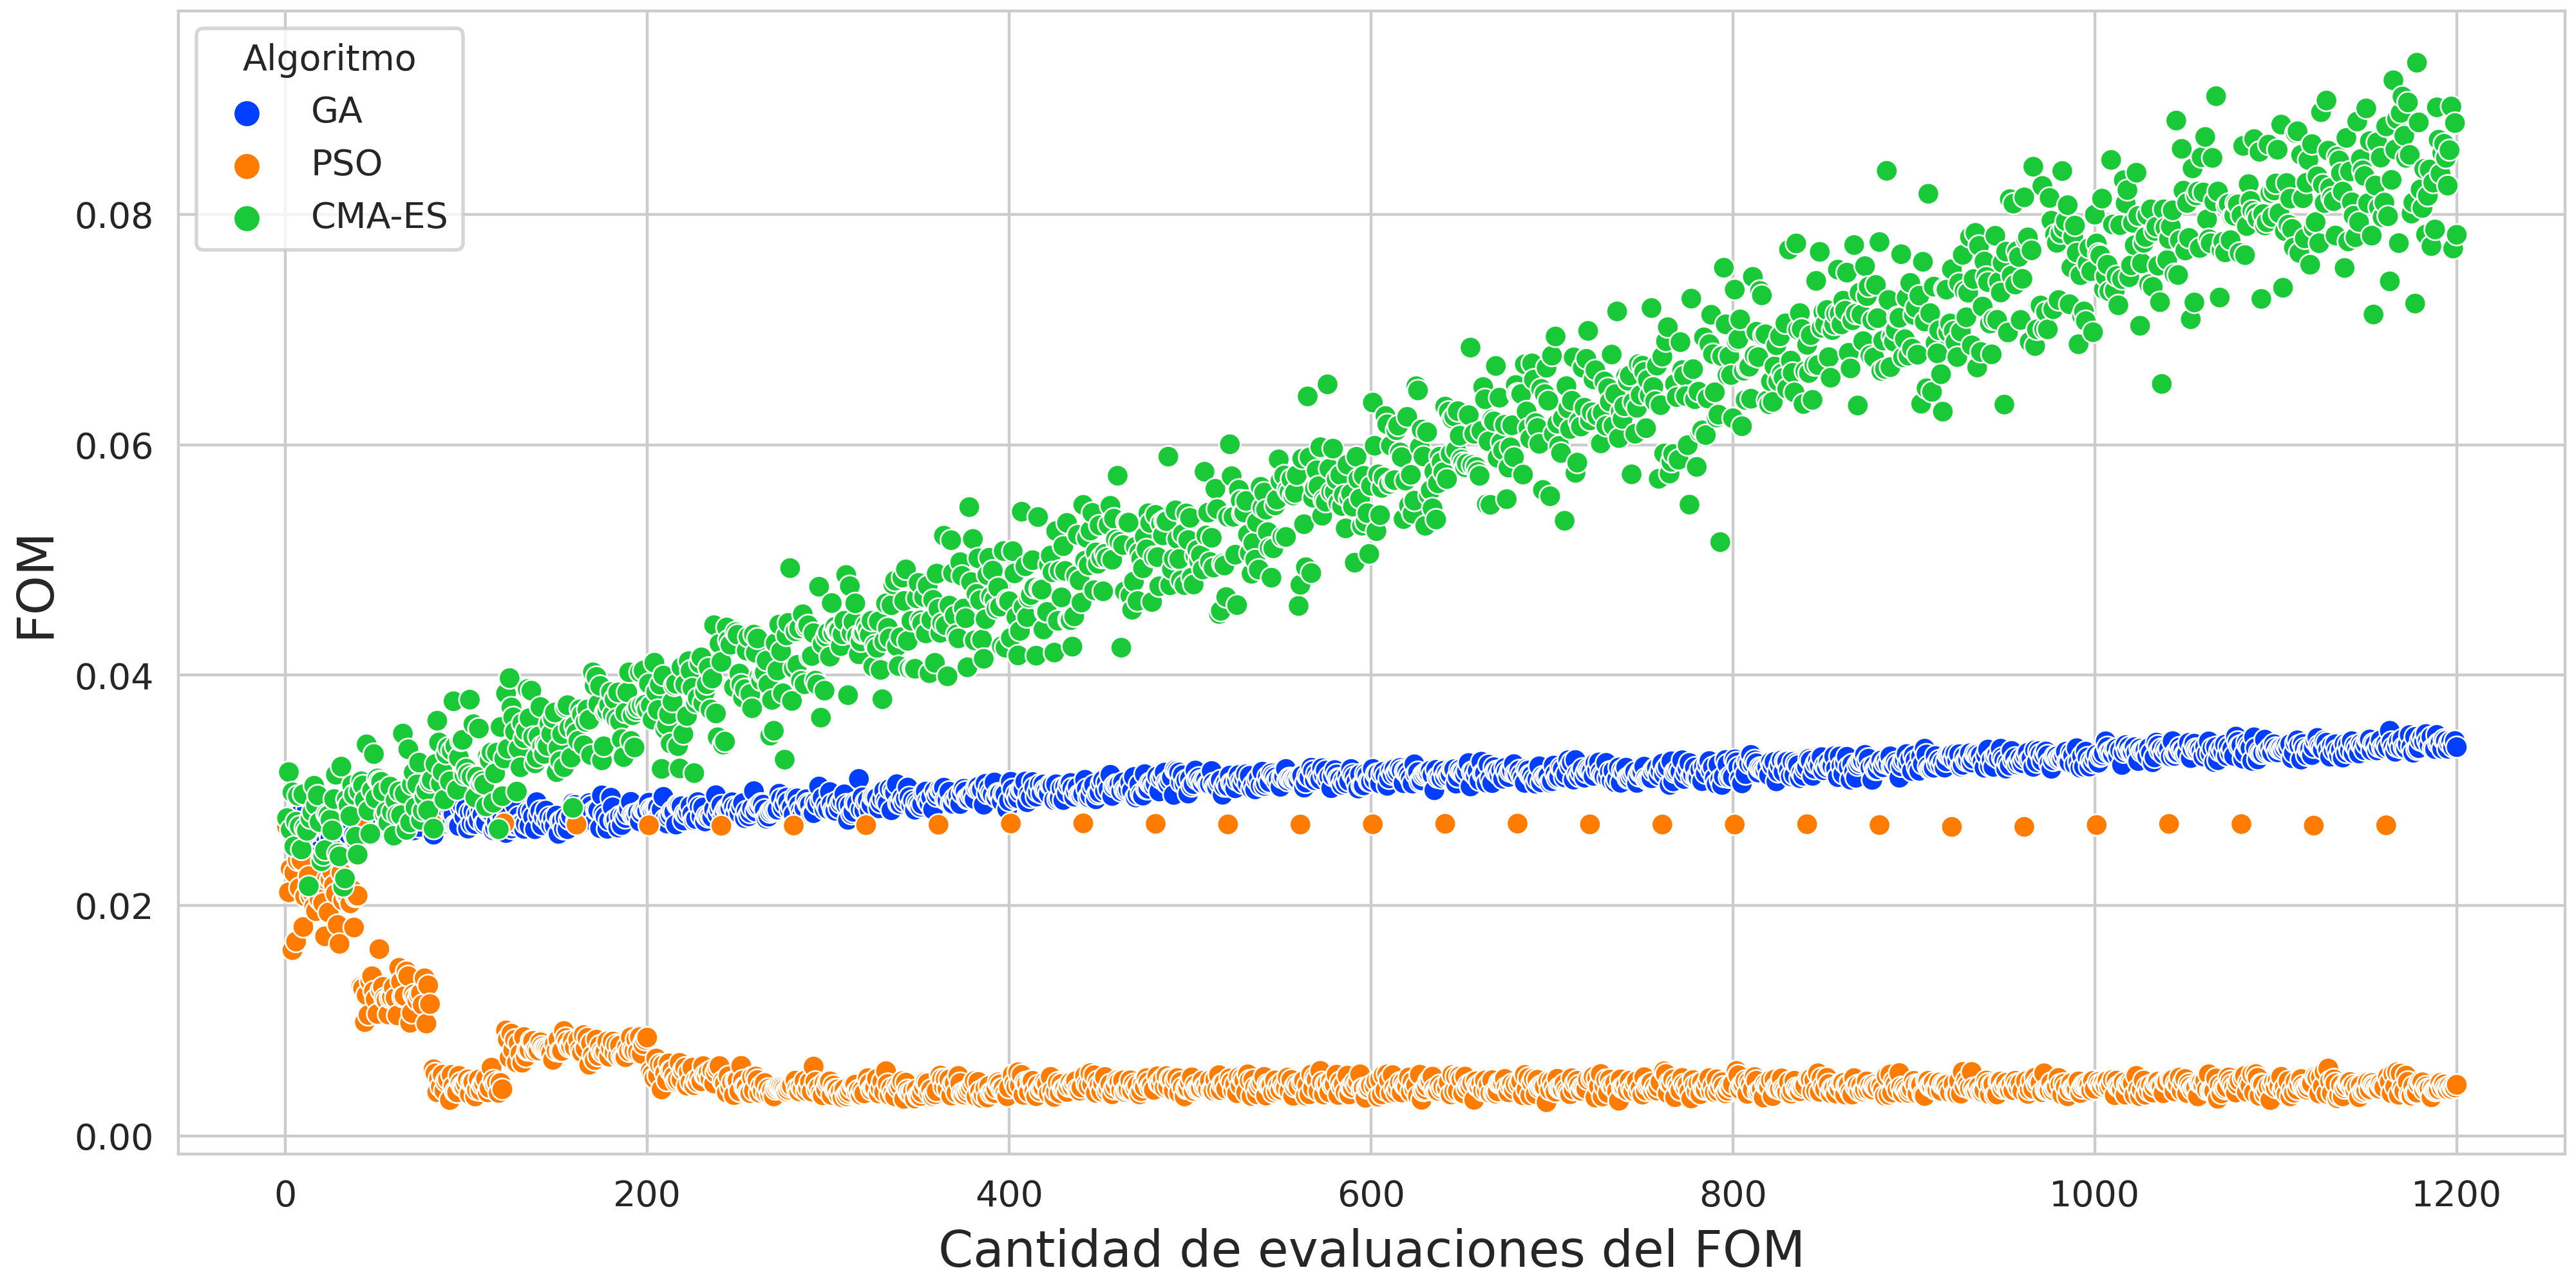
\includegraphics[width=1.0\textwidth]{image/proposal/bend-opt-cont.png}
  \caption{Comparación del desempeño de GA, PSO y CMA-ES para optimizar el \emph{bend} propuesto.}
  \label{fig:gradient-free-comparison}
\end{figure}

\begin{table}[ht]
    \centering
    \begin{tabular}{|c|c|c|}
    \hline 
    Algoritmo & Parámetro &  Valor (nm) \\
    \hline
    G-GA & population\_size & 40 \\
    G-GA & n\_selected\_parents & 10 \\
    G-GA & GA\_range & 0.1 \\
    G-GA & prob\_mutation & 0.1 \\
    G-PSO & population\_size & 40 \\
    G-PSO & PSO\_range & 0.1 \\
    G-PSO & $\omega$ & 0.5 \\
    G-PSO & $c_1$ & 0.5 \\
    G-PSO & $c_2$ & 0.5 \\
    G-CMA-ES & population\_size & 40 \\
    G-CMA-ES & $\sigma$ & 0.3 \\
    \hline 
    \end{tabular}
    \caption{Parámetros usados por los algoritmos de optimización.}
    \label{tab:alg-parameters}
\end{table}

De este modo, en esta tesis se optó por comparar solamente algoritmos de primer orden, es decir, que utilicen
el cómputo de la gradiente en sus rutinas. Así, se seguirá evaluando los algoritmos GA, PSO y CMA-ES pero
ahora en sus versiones que usan la gradiente.
Para poder comparar el desempeño de estos se configuró la máxima cantidad de veces que podían
evaluar la función objetivo. 
Los parámetros específicos con los que se ejecutaron cada algoritmo se detallan en la
\autoref{tab:alg-parameters} siguiendo la nomenclatura presentada en la \autoref{sec:alg-opt}.

Es resumen, usando simulaciones en 3D FDFD con SPINS-B, evaluamos estos cinco algoritmos:

\begin{enumerate}
  \item \textbf{G-PSO}

  Llamemos así a la versión de PSO (\autoref{sec:pso}) que usa la gradiente. 
  Basándonos en el trabajo de \cite{Demidova2020}, después de cada iteración
  del Algoritmo \ref{alg:PSO}, aplicamos el algoritmo de GD
  (\autoref{sec:gradient-descent}) para actualizar la mejor solución global encontrada por el 
  algoritmo PSO. Esta aplicación de GD se realiza por 10 iteraciones.
  La idea detrás de esta variante es asegurar que la mejor solución global alcance un buen resultado
  para lograr guiar a las demás partículas (manteniendo así el enfoque de un algoritmo de optimización
  global).
  
  Los experimentos con este algoritmo se desarrollaron con una implementación propia.

  \item \textbf{G-GA}

  Similar al G-PSO, después de cada iteración del Algoritmo \ref{alg:GA}, se escoge dos
  elementos aleatorios para actualizarlos aplicándoles GD por 10 iteraciones.
  Se escoge dos elementos y no solo uno para asegurar que los resultados de aplicar GD
  se compartan rápidamente con los demás individuos en pocas iteraciones.

  Los experimentos con este algoritmo se desarrollaron con una implementación propia.

  \item \textbf{G-CMA-ES}

  En esta variante, al final de cada iteración del Algoritmo \ref{alg:CMA} se
  calcula la gradiente de la media obtenida, luego este valor se utiliza para
  actualizar la hiperelipse en la siguiente iteración.
  Los detalles precisos se pueden encontrar en \cite{Nikolaus2021}.

  Los experimentos con este algoritmo se desarrollaron usando el paquete de Python pycma
  \citep{hansen2019pycma}.

  \item \textbf{MMA} (\autoref{sec:mma})

  No se realizaron variantes en este algoritmo.
  Los experimentos se desarrollaron usando el paquete de Python NLOpt \citep{nlopt}.

  \item \textbf{L-BFGS-B} (\autoref{sec:lbfgsb})

  No se realizaron variantes en este algoritmo.
  Los experimentos se desarrollaron usando el paquete de Python SciPy \citep{2020SciPy-NMeth}.

\end{enumerate}

A continuación, se detalla la estrategia de optimización seguida en este trabajo.
Esta propuesta esta inspirada (principalmente) en el trabajo de \cite{Su2020} y \cite{Christiansen2021}.
En cada una de estas etapas se limitó la cantidad de veces que se podía evaluar $f_{obj}$ para su
posterior comparación. Además, para G-GA y G-PSO se agregó una condición para terminar el algoritmo
en caso de no encontrar mejoras mayores a $10^{-9}$ en las últimas $5$ iteraciones, 
para el L-BFGS-B se usó valores por defecto y para $MMA$ se estableció un tolerancia relativa de $10^{-9}$.

\section{Optimización Continua}

En esta etapa se configuró la máxima cantidad de evaluaciones a 2000.
Luego, se ejecutaron los cinco algoritmos para optimizar el \emph{bend} y WDM.
Cada algoritmo se ejecutó 3 veces, la primera con un valor de semilla de 128, la segunda de 256 y
la tercera de 512.
La idea de esta etapa es optimizar los diseños sin imponer ninguna restricción.
Es decir, directamente usamos la parametrización $\boldsymbol{P}$ para evaluar la permitividad 
$\varepsilon$ (\autoref{eq:permitivity}),
lo cual lo podemos representar como $(\boldsymbol{P} \mathrel{\leadsto} \varepsilon)$.

\section{Optimización Discreta}

Los objetivos de esta etapa son dos: (i) obtener diseños con un mínimo radio de curvatura $r_f$ e
(ii) ir eliminando las regiones grises.
Para el primer objetivo se aplicó la \autoref{eq:densityfilter} a la parametrización 
$\boldsymbol{P}$ usando un radio de curvatura $r_f = 80 nm$.
Como $80nm$ es igual a 5 veces el tamaño de los píxeles configurados en la \autoref{sec:preparar-simulacion},
solamente fue necesario explorar una submatriz de $11 \times 11$ alrededor de cada elemento para el cálculo de
esta ecuación.
Para el segundo objetivo se aplicó la \autoref{eq:projection} al resultado conseguido por el anterior filtro.
Este proceso lo podemos representar como 
$(\boldsymbol{P} \mathrel{\leadsto} \widetilde{\boldsymbol{P}} \mathrel{\leadsto}
\widetilde{\widetilde{\boldsymbol{P}}} \mathrel{\leadsto} \varepsilon)$.

Para la optimización se utilizó los resultados de la optimización continua como punto inicial.
Para ello se realizó una primera optimización configurando la máxima cantidad de evaluaciones 
en 800 y aplicando a cada diseño los filtros descritos anteriormente con $\beta = 2^1$ y $\eta = 0.5$
para la \autoref{eq:projection}.
El resultado de esta optimización se usa como punto inicial para repetir este proceso, pero ahora con $\beta
= 2^2$. Finalmente, se repite una vez más el procedimiento con $\beta = 2^3$.

\section{Optimización de Fabricación}

Por último, se busca imponer a los diseños restricciones de fabricación y robustez a posibles errores
de fabricación. 

Tomando como referencia el trabajo de \cite{Hammond20} para asegurar un buen desempeño pese a los errores de
fabricación, por cada parametrización $\boldsymbol{P}$ se calculó:

\begin{itemize}
  \item $\widetilde{\widetilde{\boldsymbol{P}}}_{d}$ que representa el diseño como si el dispositivo se hubiera dilatado.
  \item $\widetilde{\widetilde{\boldsymbol{P}}}_{i}$ que representa el diseño normal.
  \item $\widetilde{\widetilde{\boldsymbol{P}}}_{e}$  que representa el diseño como si el dispositivo se
    hubiera expandido.
\end{itemize}

Estos tres elementos se calcularon siguiendo los mismos filtros descritos en la anterior sección
$(\boldsymbol{P} \mathrel{\leadsto} \widetilde{\boldsymbol{P}} \mathrel{\leadsto}
\widetilde{\widetilde{\boldsymbol{P}}} \mathrel{\leadsto} \varepsilon)$.
Pero, para el diseño dilatado se usó $\eta_d = 0.45$, para el diseño normal $\eta_i = 0.5$ y
para el diseño expandido $\eta_e = 0.55$.

Luego, se definió una nueva función objetivo mediante la siguiente ecuación:

\begin{equation}
  \begin{split}
    F_{obj} = max(min(
    f_{obj}(\widetilde{\widetilde{\boldsymbol{P}}}_{d}),
    f_{obj}(\widetilde{\widetilde{\boldsymbol{P}}}_{i}),
    f_{obj}(\widetilde{\widetilde{\boldsymbol{P}}}_{e})
    )
  \end{split}
  \label{eq:final-fom}
\end{equation}

Así, considerando el peor escenario ante dos posibles errores de fabricación (expansión o contracción),
se busca el diseño más robusto posible.
Para optimizar esta nueva función objetivo se realizó el mismo proceso de la optimización discreta, pero ahora
con valores $\beta = 2^4, 2^5, 2^6$ y limitando a 400 evaluaciones de $F_{obj}$ por cada $\beta$. 
De esta manera, en paralelo, seguimos con el proceso de discretizar
nuestros resultados.

\section{Preparación para Fabricación}

Finalmente, se seleccionó el diseño más optimo obtenido para un \emph{bend} y WDM.
Luego, se realizó un análisis del funcionamiento de estos dispositivos a distintas longitudes de onda
y se evaluó su desempeño al eliminar regiones aisladas.
Para la eliminación de regiones aisladas se realizó una búsqueda por profundidad
desde la intersección entre la guía de entrada y la región de diseño.
Para ello recorrimos la matriz $\boldsymbol{P}$ como un grafo implícito moviéndonos a una celda
vecina si está poseía un valor mayor a 0.5.

%Posteriormente, usando la permitividad asociada a sus parametrization se obtuvo la geometría del dispositivo.
%Esta geometría se aproximó mediante polígonos usando el paquete \emph{mathplotlib} de Python
%para representar el diseño en formato GDSII y dejarlo listo para fabricación.

\section{Alcances y Limitaciones}

El presente trabajo solo se realizó mediante simulaciones computacionales, no se llegó a la parte de
fabricación por temas de tiempo y presupuesto. Sin embargo, los mejores diseños optimizados se
encuentran listos para poder ser fabricados.

En este capítulo hemos explicado los seis pasos seguidos en esta tesis.
Primero, comenzamos describiendo la configuración de nuestros dispositivos a optimizar.
Segundo, se detalló los cinco algoritmos a utilizar, sus parámetros y justificación de elección.
Luego, se desarrolló la estrategia de optimización a seguir: optimización continua, discreta y de fabricación.
Finalmente, se describió la etapa final realizada con los mejores diseños obtenidos.

%\chapter{Experimentaciones y Resultados}\label{chapter:results}

En la presente sección comenzaremos mostrando los sistemas de cómputo utilizados para la experimentación.
Seguidamente, dividimos este capítulo en seis secciones.
Primero, se muestra los resultados de la optimización del \emph{bend}.
Para ello se inicia mostrando en tres gráficas distintas el desempeño de cada algoritmo en 
las tres etapas de la estrategia de optimización; luego se detalla los resultados por cada algoritmo
de manera individual.
Segundo, se realiza un análisis al diseño del \emph{bend} mejor optimizado.
Tercero, de manera similar al caso del \emph{bend}, se expone los resultado de la optimización del WDM.
Cuarto, se desarrolla un análisis al diseño del WDM mejor optimizado.
Quinto, se realiza una discusión crítica sobre los resultados de la optimización del \emph{bend}.
Finalmente, se realiza una discusión similar sobre los resultados del WDM.

Los experimentos se realizaron en tres equipos brindados por la Universidad de Ingeniería y Tecnología:

\begin{enumerate}
  \item Un Intel Core i7-3770K 3.50 GHz con 8 cores y 32 GB de RAM.
        Este computador contó con un GPU NVIDIA Quadro RTX 4000 con 8GB GDDR6.

  \item Del \emph{cluster} Khipu, un Intel Xeon Gold 6230 2.10 GHz con 40 \emph{cores} y 128 GB de RAM.
        Este nodo contó con un GPU NVIDIA Tesla T4 con 16 GB GDDR6.

  \item Del \emph{cluster} Khipu, un AMD EPYC 7742 2.25 GHz con 128 \emph{cores} y 1024 GB de RAM.
        Este nodo contó con un GPU NVIDIA Ampere A100 con 40 GB HMB2.

\end{enumerate}

Sacando la media geométrica de los tiempos calculados, el tiempo promedio de ejecución en los tres 
sistemas en cada etapa de la estrategia de optimización se detalla en la \autoref{tab:times} (el signo -
indica que en ese sistema de cómputo no se realizaron experimentos con ese dispositivo).

\begin{table}[ht]
    \centering
    \begin{tabular}{|c|c|c|c|}
    \hline 
      Tiempo promedio &  Quadro RTX (s) & Tesla T4 & Ampere A100 \\
    \hline 
      Optimización continua (\emph{bend})            & 14.261 & 15.432 & - \\
      Optimización discreta (\emph{bend})            & 15.961 & 18.718 & - \\
      Optimización de fabricación (\emph{bend})      & 47.084 & 50.639 & - \\
      Optimización continua (WDM)                    & 16.876 & - & 17.479 \\
      Optimización discreta (WDM)                    & 18.431 & - & 19.780 \\
      Optimización de fabricación (WDM)              & 53.941 & - & 55.406 \\
    \hline 
    \end{tabular}
    \caption{Tiempos promedios de ejecución en cada etapa de optimización para el \emph{bend} y WDM con los
    tres sistemas de cómputo usados.}
    \label{tab:times}
\end{table}

Por cada optimización se realizó como máximo $2000$ evaluaciones de $f_{obj}$ en la optimización continua,
$3 \times 800$ en la optimización discreta y $3 \times 400$ en la optimización de fabricación.
Así, por ejemplo, usando Quadro RTX la optimización de un \emph{bend} podía tomar hasta 34 horas
y usando Ampere A100 la optimización de un WDM podía tomar hasta 41 horas.

Por otro lado, cada GPU solo puede realizar una simulación a la vez, en caso de querer 
evaluar dos parametrizaciones al mismo tiempo una era puesta en cola. De este modo,
siendo el tiempo de simulación el cuello de botella de las optimizaciones, los programas simplemente
se ejecutaron con un solo \emph{core} y se limitó la memoria a 32 GB para los nodos del \emph{cluster}
Khipu mediante SLURM (herramienta que funciona como gestor de recursos de Khipu).


En las siguientes secciones las imágenes que muestran resultados del \emph{bend} o WDM
incluyen un círculo blanco, este representa una circunferencia de radio $r_f = 80 nm$,
el mínimo radio de curvatura que se está intentando imponer.


\section{Resultados de Optimización del \emph{Bend}}\label{sec:results-bend}

% \iffalse % FLAG

En la \autoref{fig:bend-cont}, \autoref{fig:bend-disc} y \autoref{fig:bend-fab} se observa 
el desempeño de los cinco algoritmos seleccionados en la etapa de optimización continua, discreta y
de fabricación del \emph{bend}, respectivamente.
Los resultados en más detalle por algoritmo se pueden encontrar en la 
\autoref{tab:opt-LBFGSB-bend} (L-BFGS-B),
\autoref{tab:opt-CMA-bend} (G-CMA-ES),
\autoref{tab:opt-MMA-bend} (MMA),
\autoref{tab:opt-PSO-bend} (G-PSO) y
\autoref{tab:opt-GA-bend} (G-GA).

\begin{landscape}
\begin{figure}[ht]
  \centering
  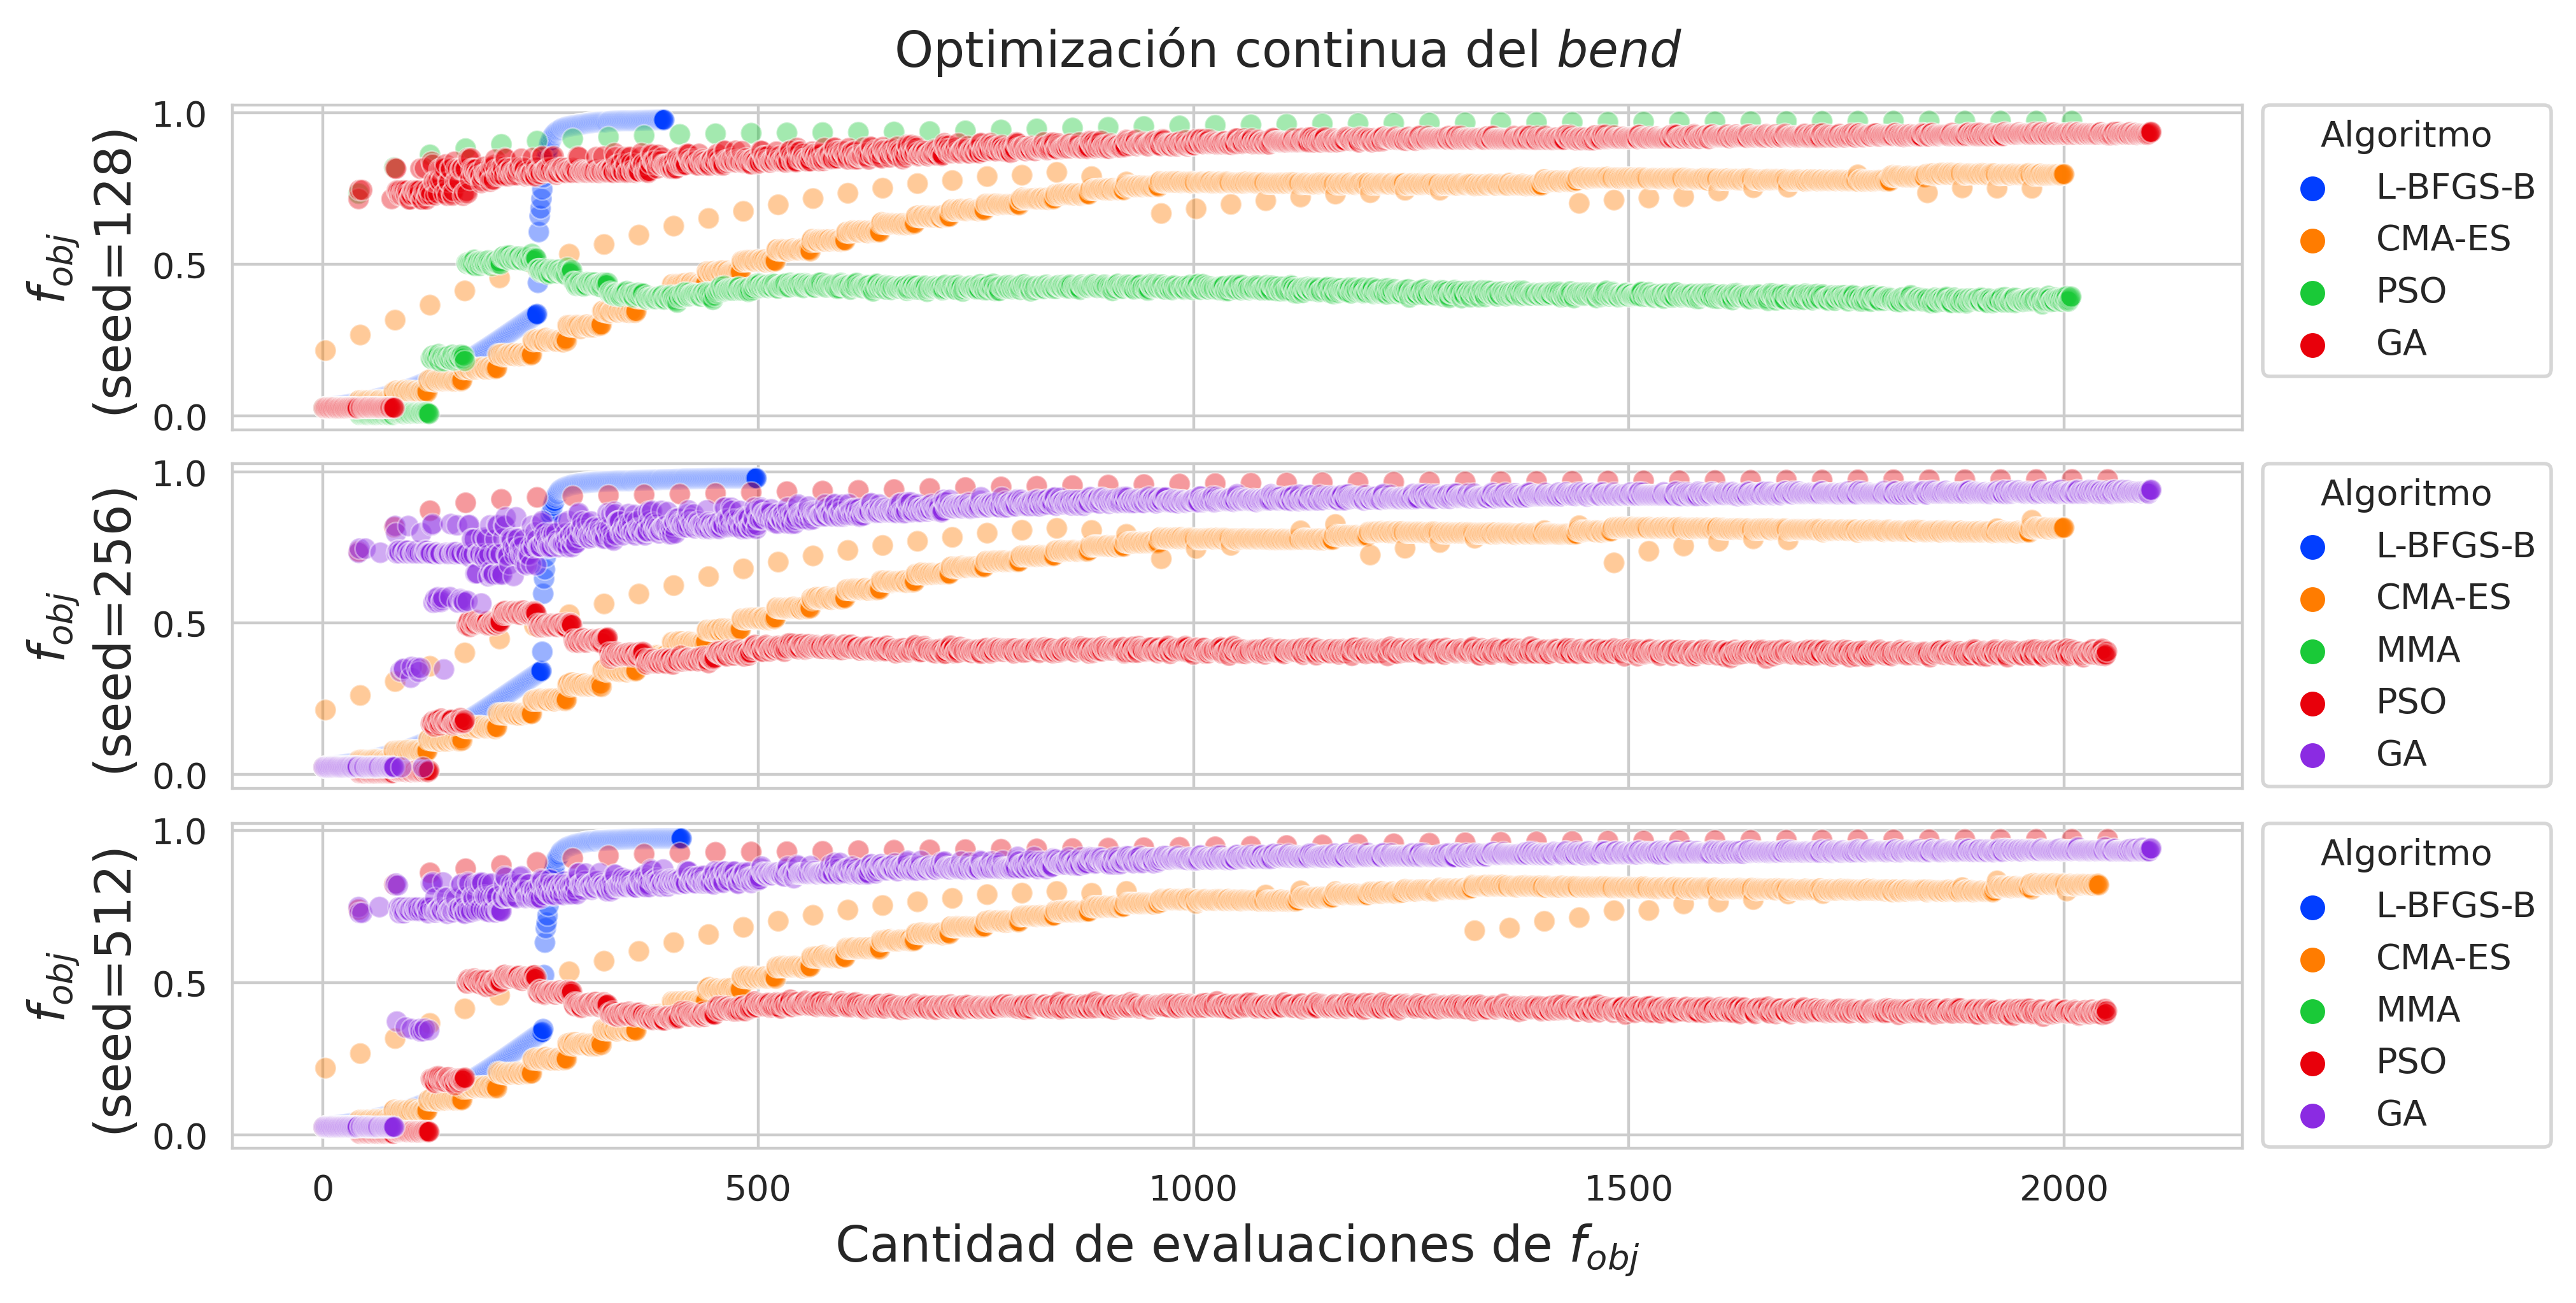
\includegraphics[scale=1.0]{image/results/bend/bend-opt-cont.png}
  \caption{Gráfico de valores de $f_{obj}$ obtenidos por los algoritmos en la optimización continua del \emph{bend}}
  \label{fig:bend-cont}
\end{figure}
\end{landscape}

\begin{landscape}
\begin{figure}[ht]
  \centering
  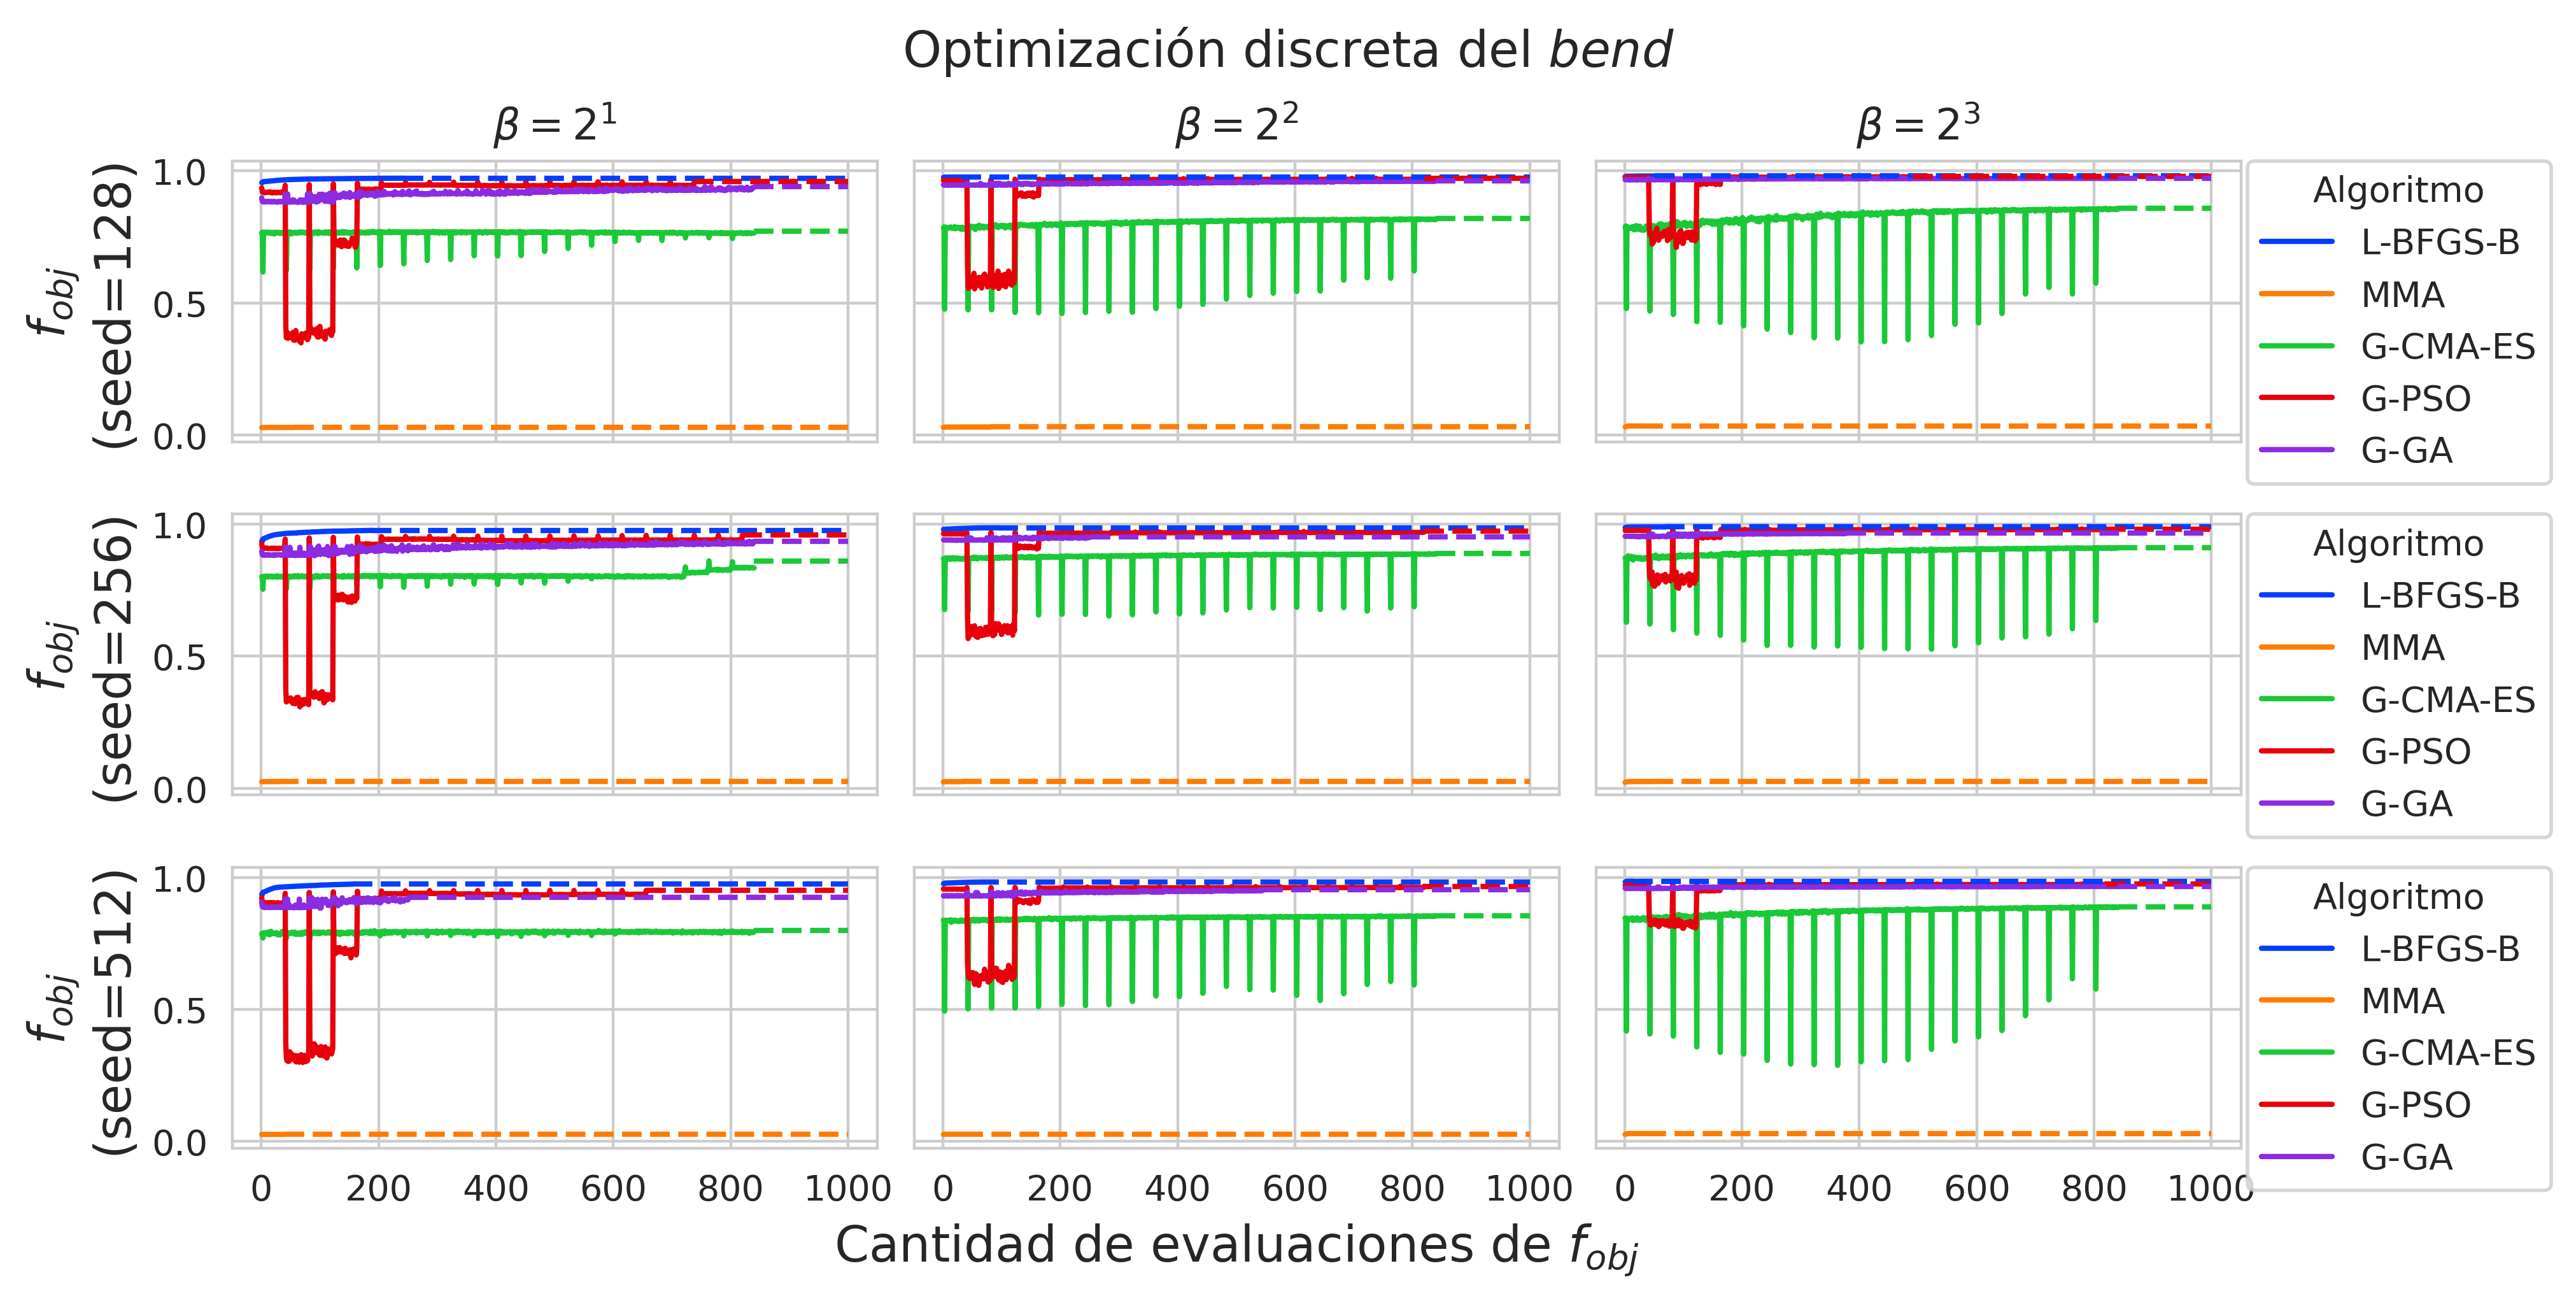
\includegraphics[scale=1.0]{image/results/bend/bend-opt-disc.png}
  \caption{Gráfico de valores de $f_{obj}$ obtenidos por los algoritmos en la optimización discreta del \emph{bend}}
  \label{fig:bend-disc}
\end{figure}
\end{landscape}

\begin{landscape}
\begin{figure}[ht]
  \centering
  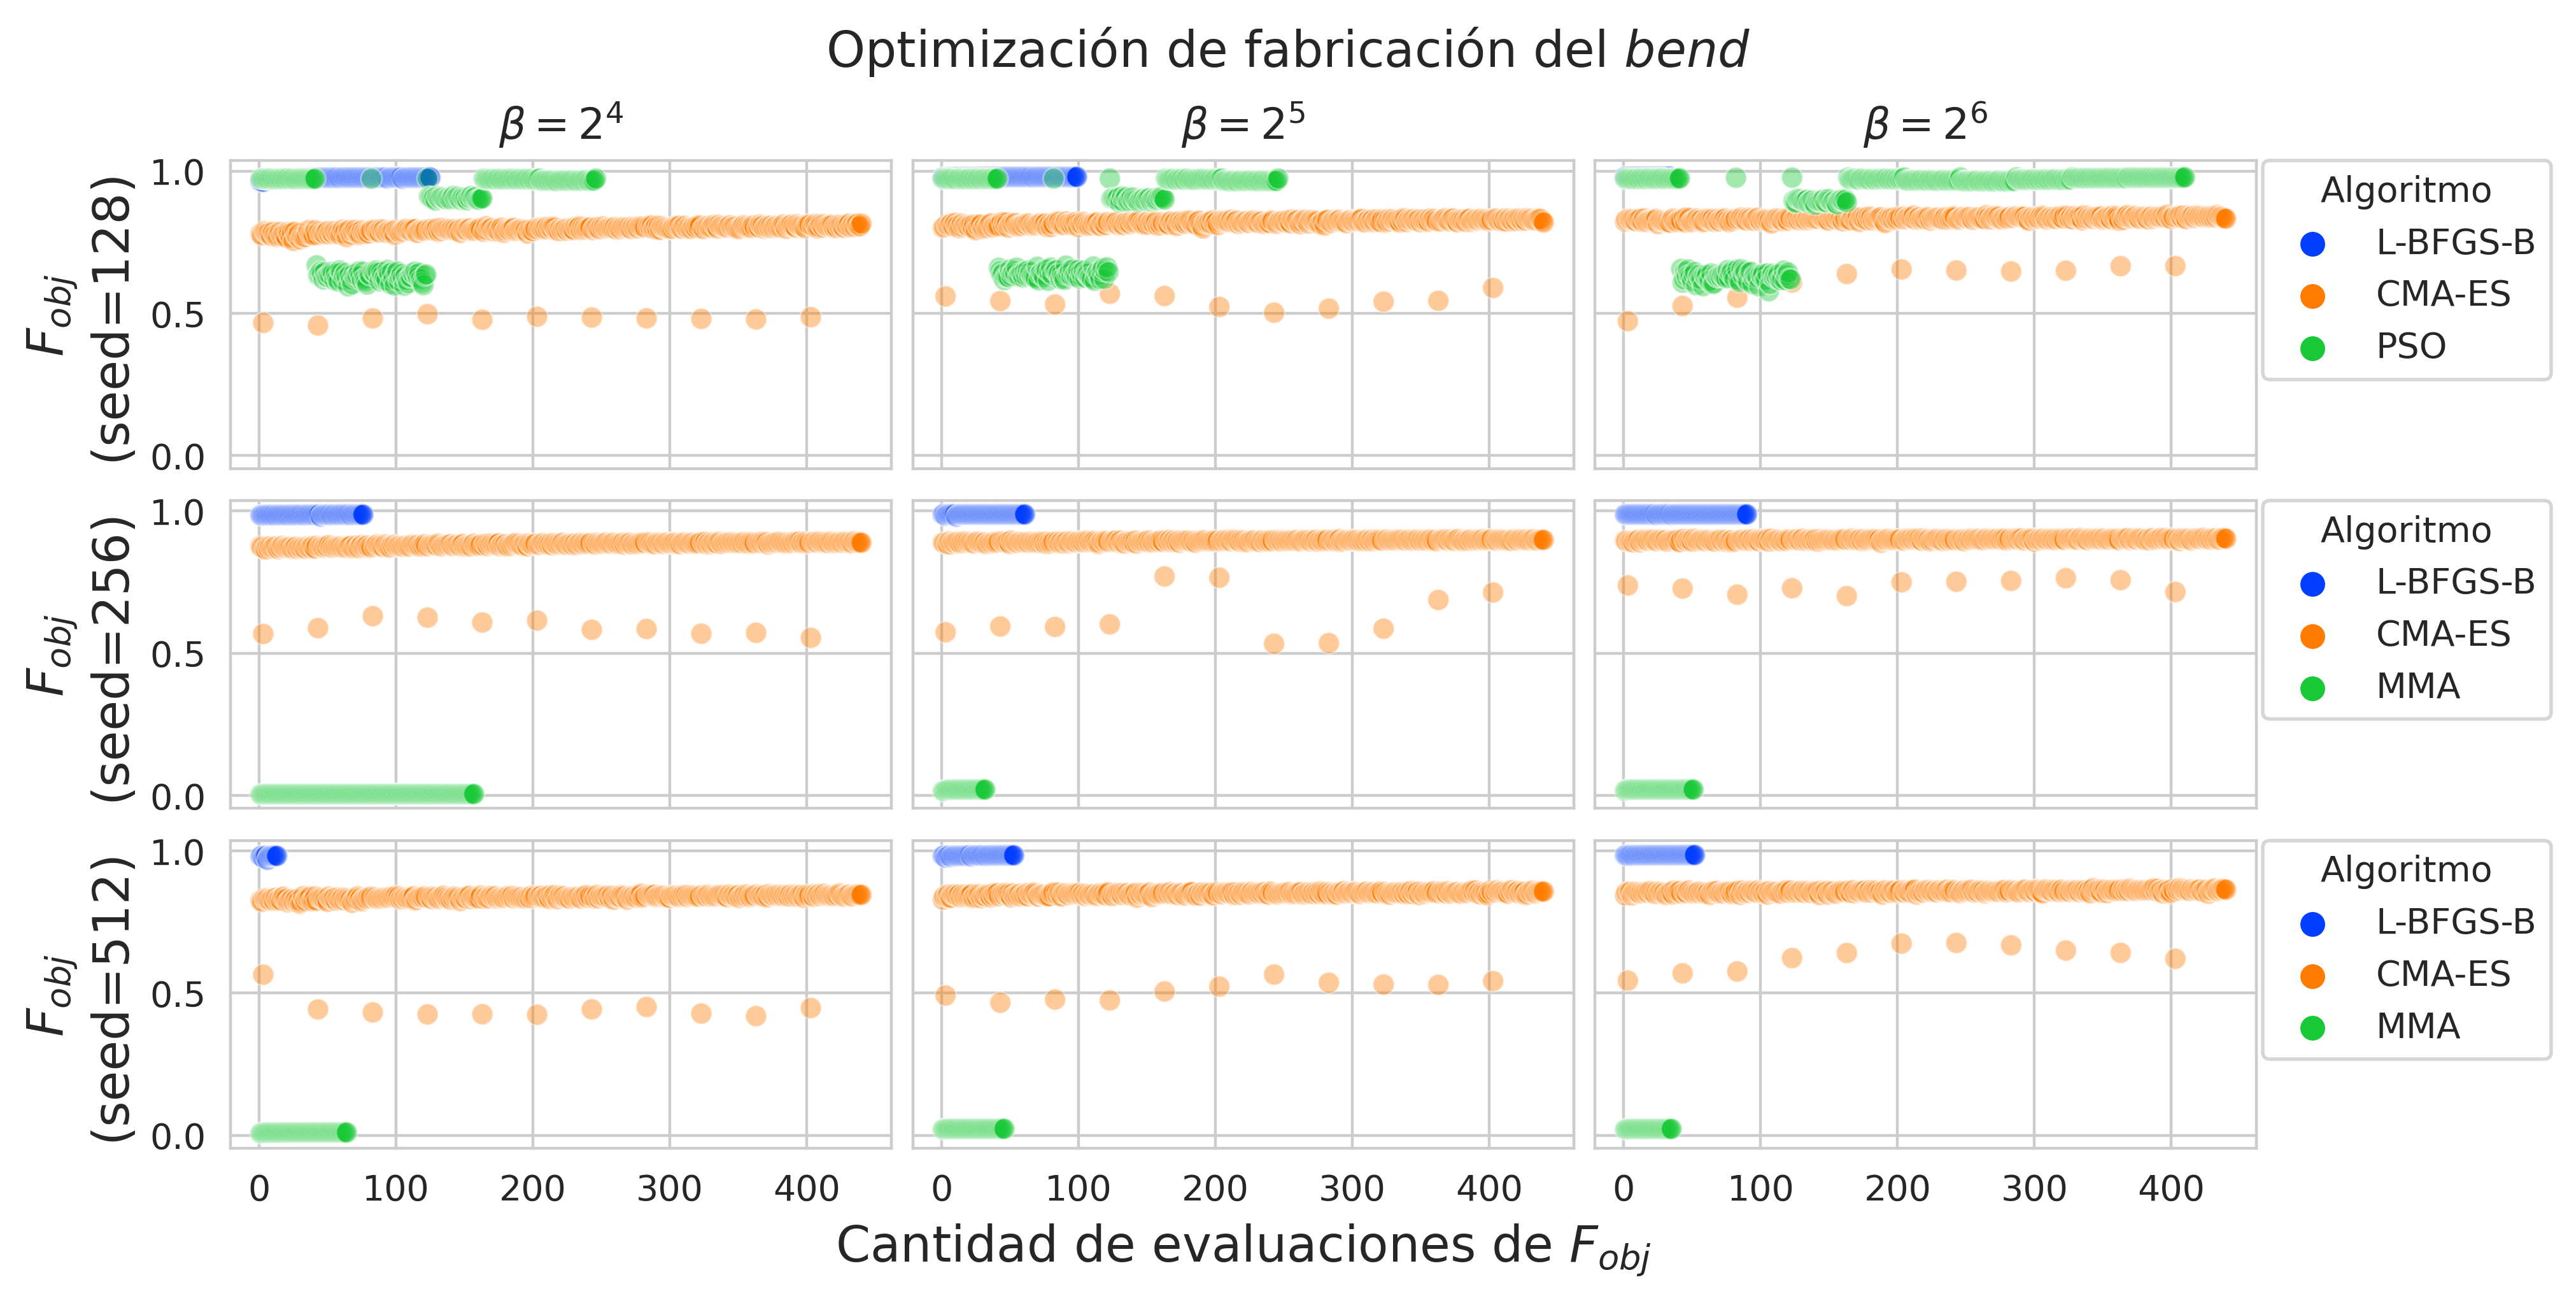
\includegraphics[scale=1.0]{image/results/bend/bend-opt-fab.png}
  \caption{Gráfico de valores de $F_{obj}$ obtenidos por los algoritmos en la optimización de fabricación del \emph{bend}}
  \label{fig:bend-fab}
\end{figure}
\end{landscape}

% Bend - L-BFGS-B
\begin{table}[ht]
    \centering
    \vspace*{-2.5cm}
    \hspace*{-3cm}
    \begin{tabular}{|c|c|c|c|}
    \hline 
    \emph{Seed} & Opt. continua & Opt. discreta &  Opt. de fabricación \\
    \hline
      \multirow{2}{*}{128} &
      
\includegraphics[width=0.20\textwidth]{image/results/bend/L-BFGS-B/visualize_eps_cont_128.png} &
      
\includegraphics[width=0.20\textwidth]{image/results/bend/L-BFGS-B/visualize_eps_disc_128.png} &
      
\includegraphics[width=0.20\textwidth]{image/results/bend/L-BFGS-B/visualize_eps_fab_128.png} \\
      \cline{2-4}
      &
      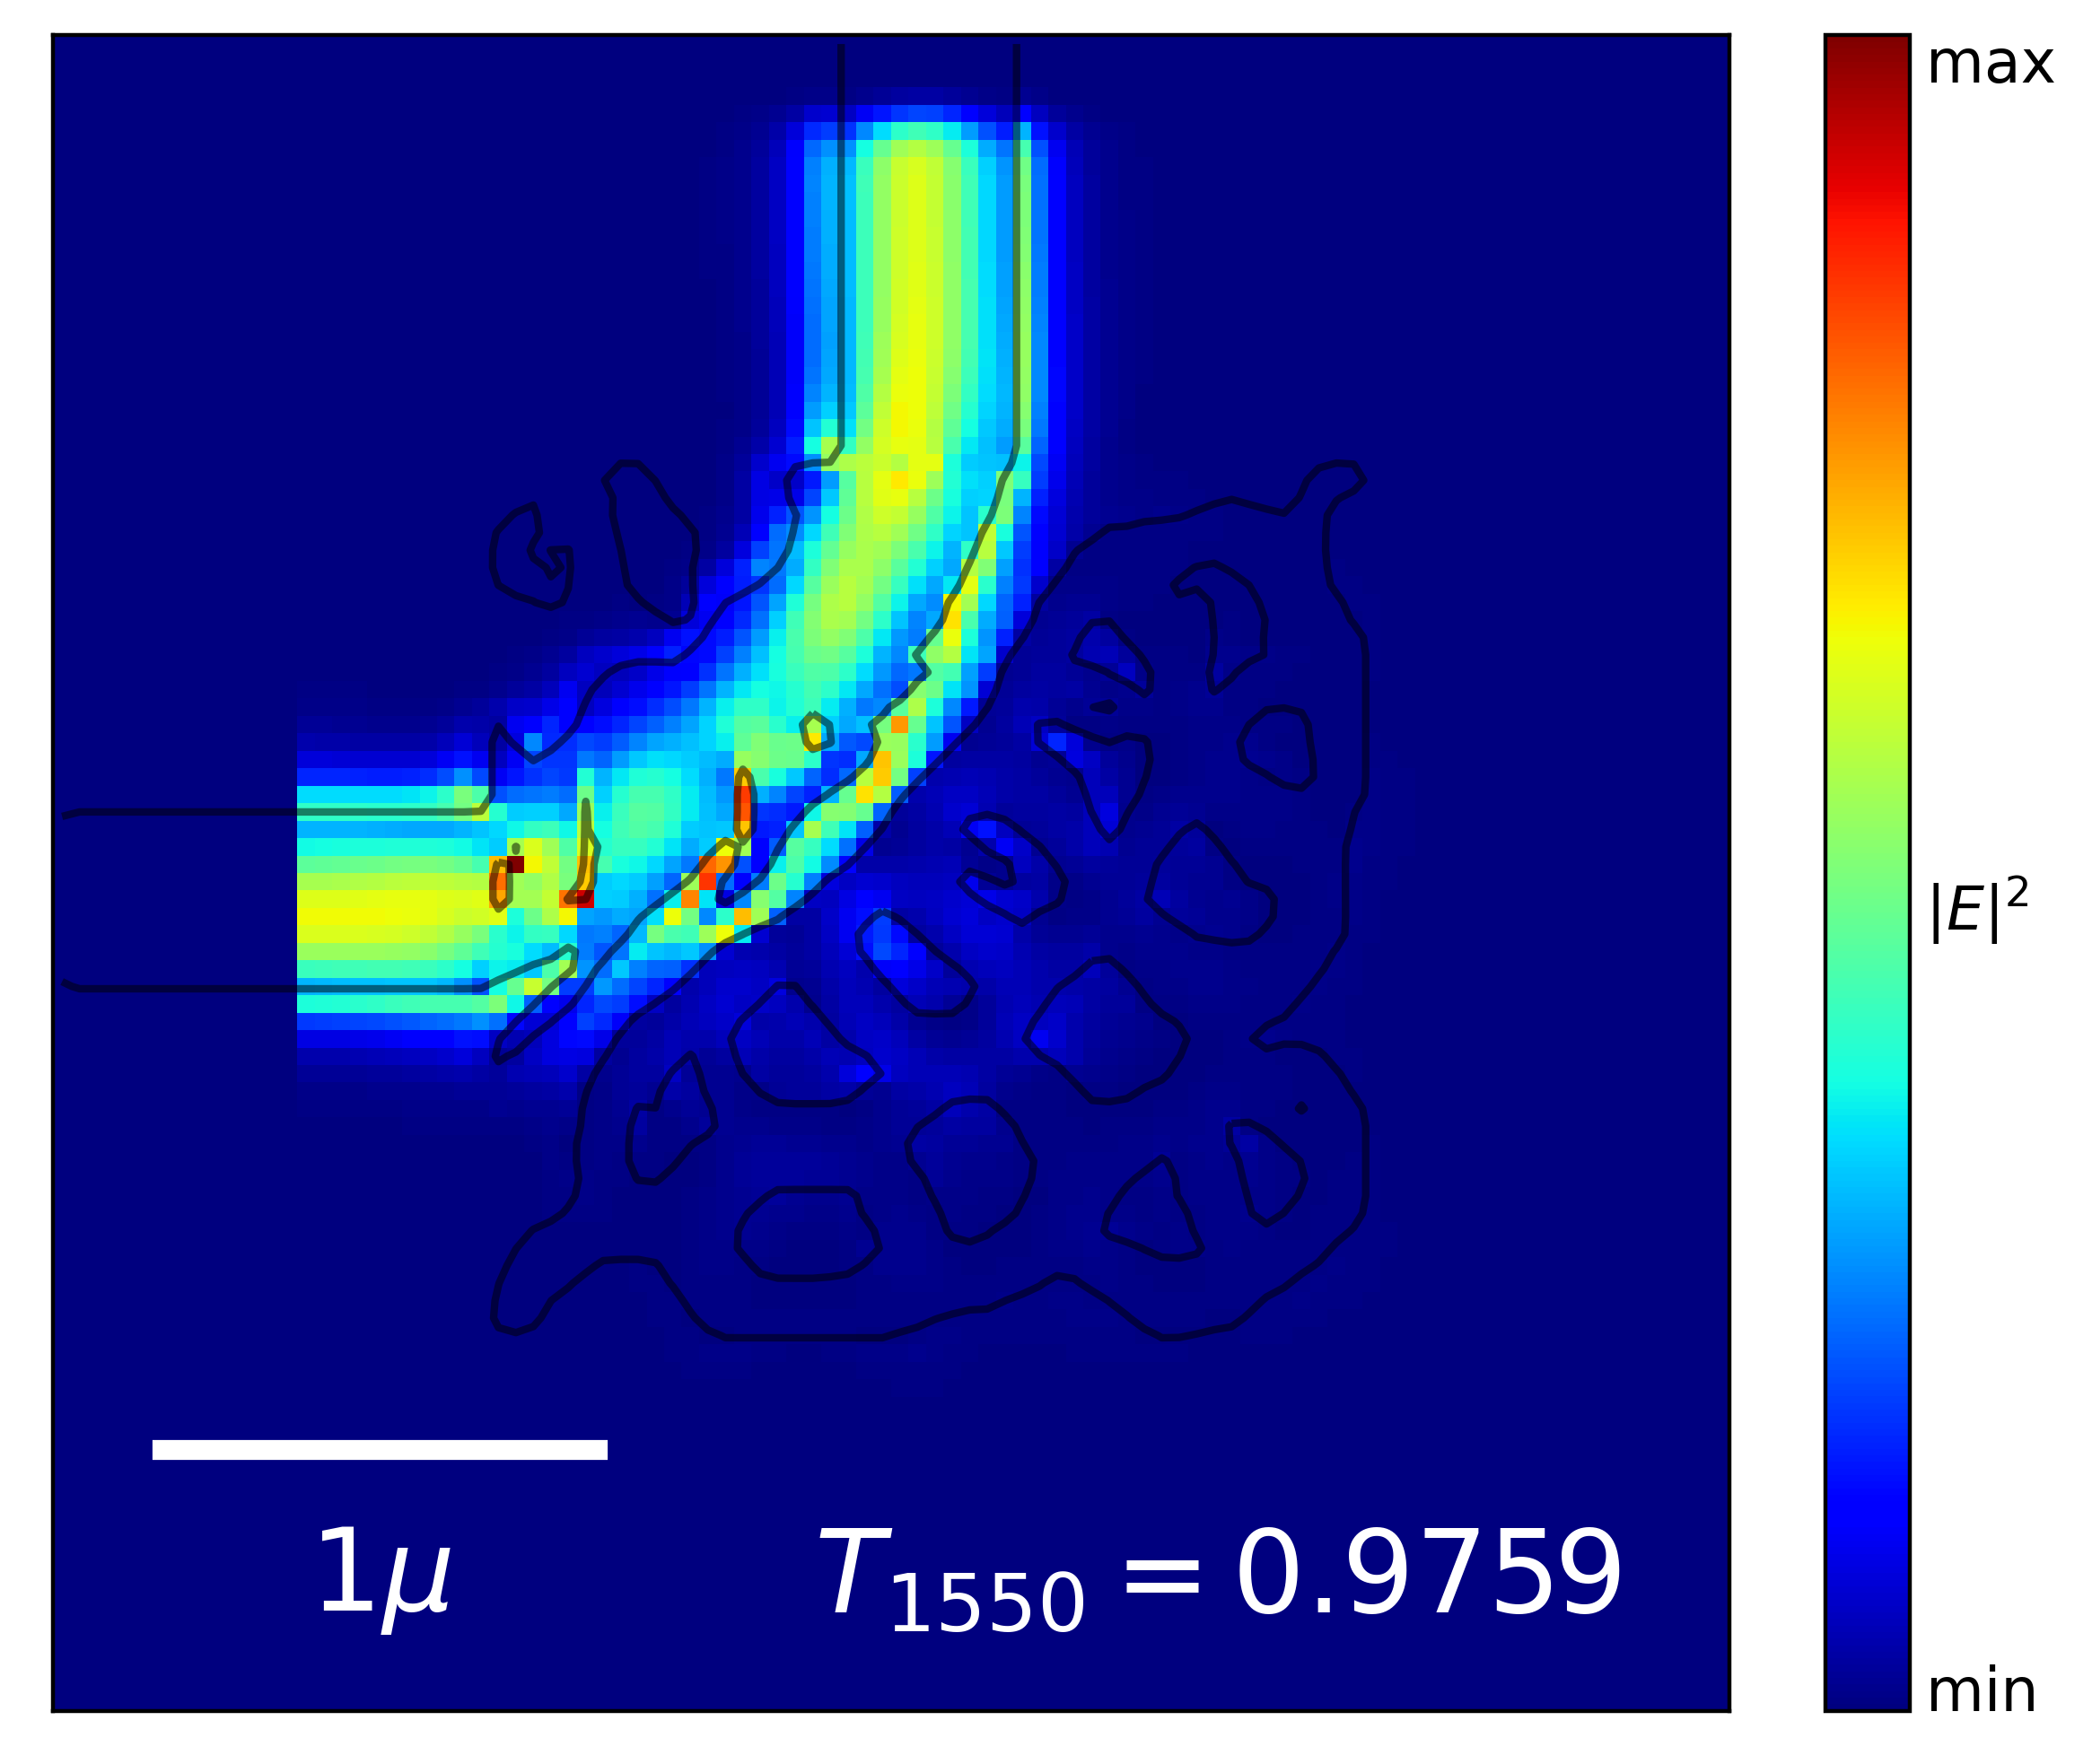
\includegraphics[width=0.33\textwidth]{image/results/bend/L-BFGS-B/visualize_field_cont_128.png} &
      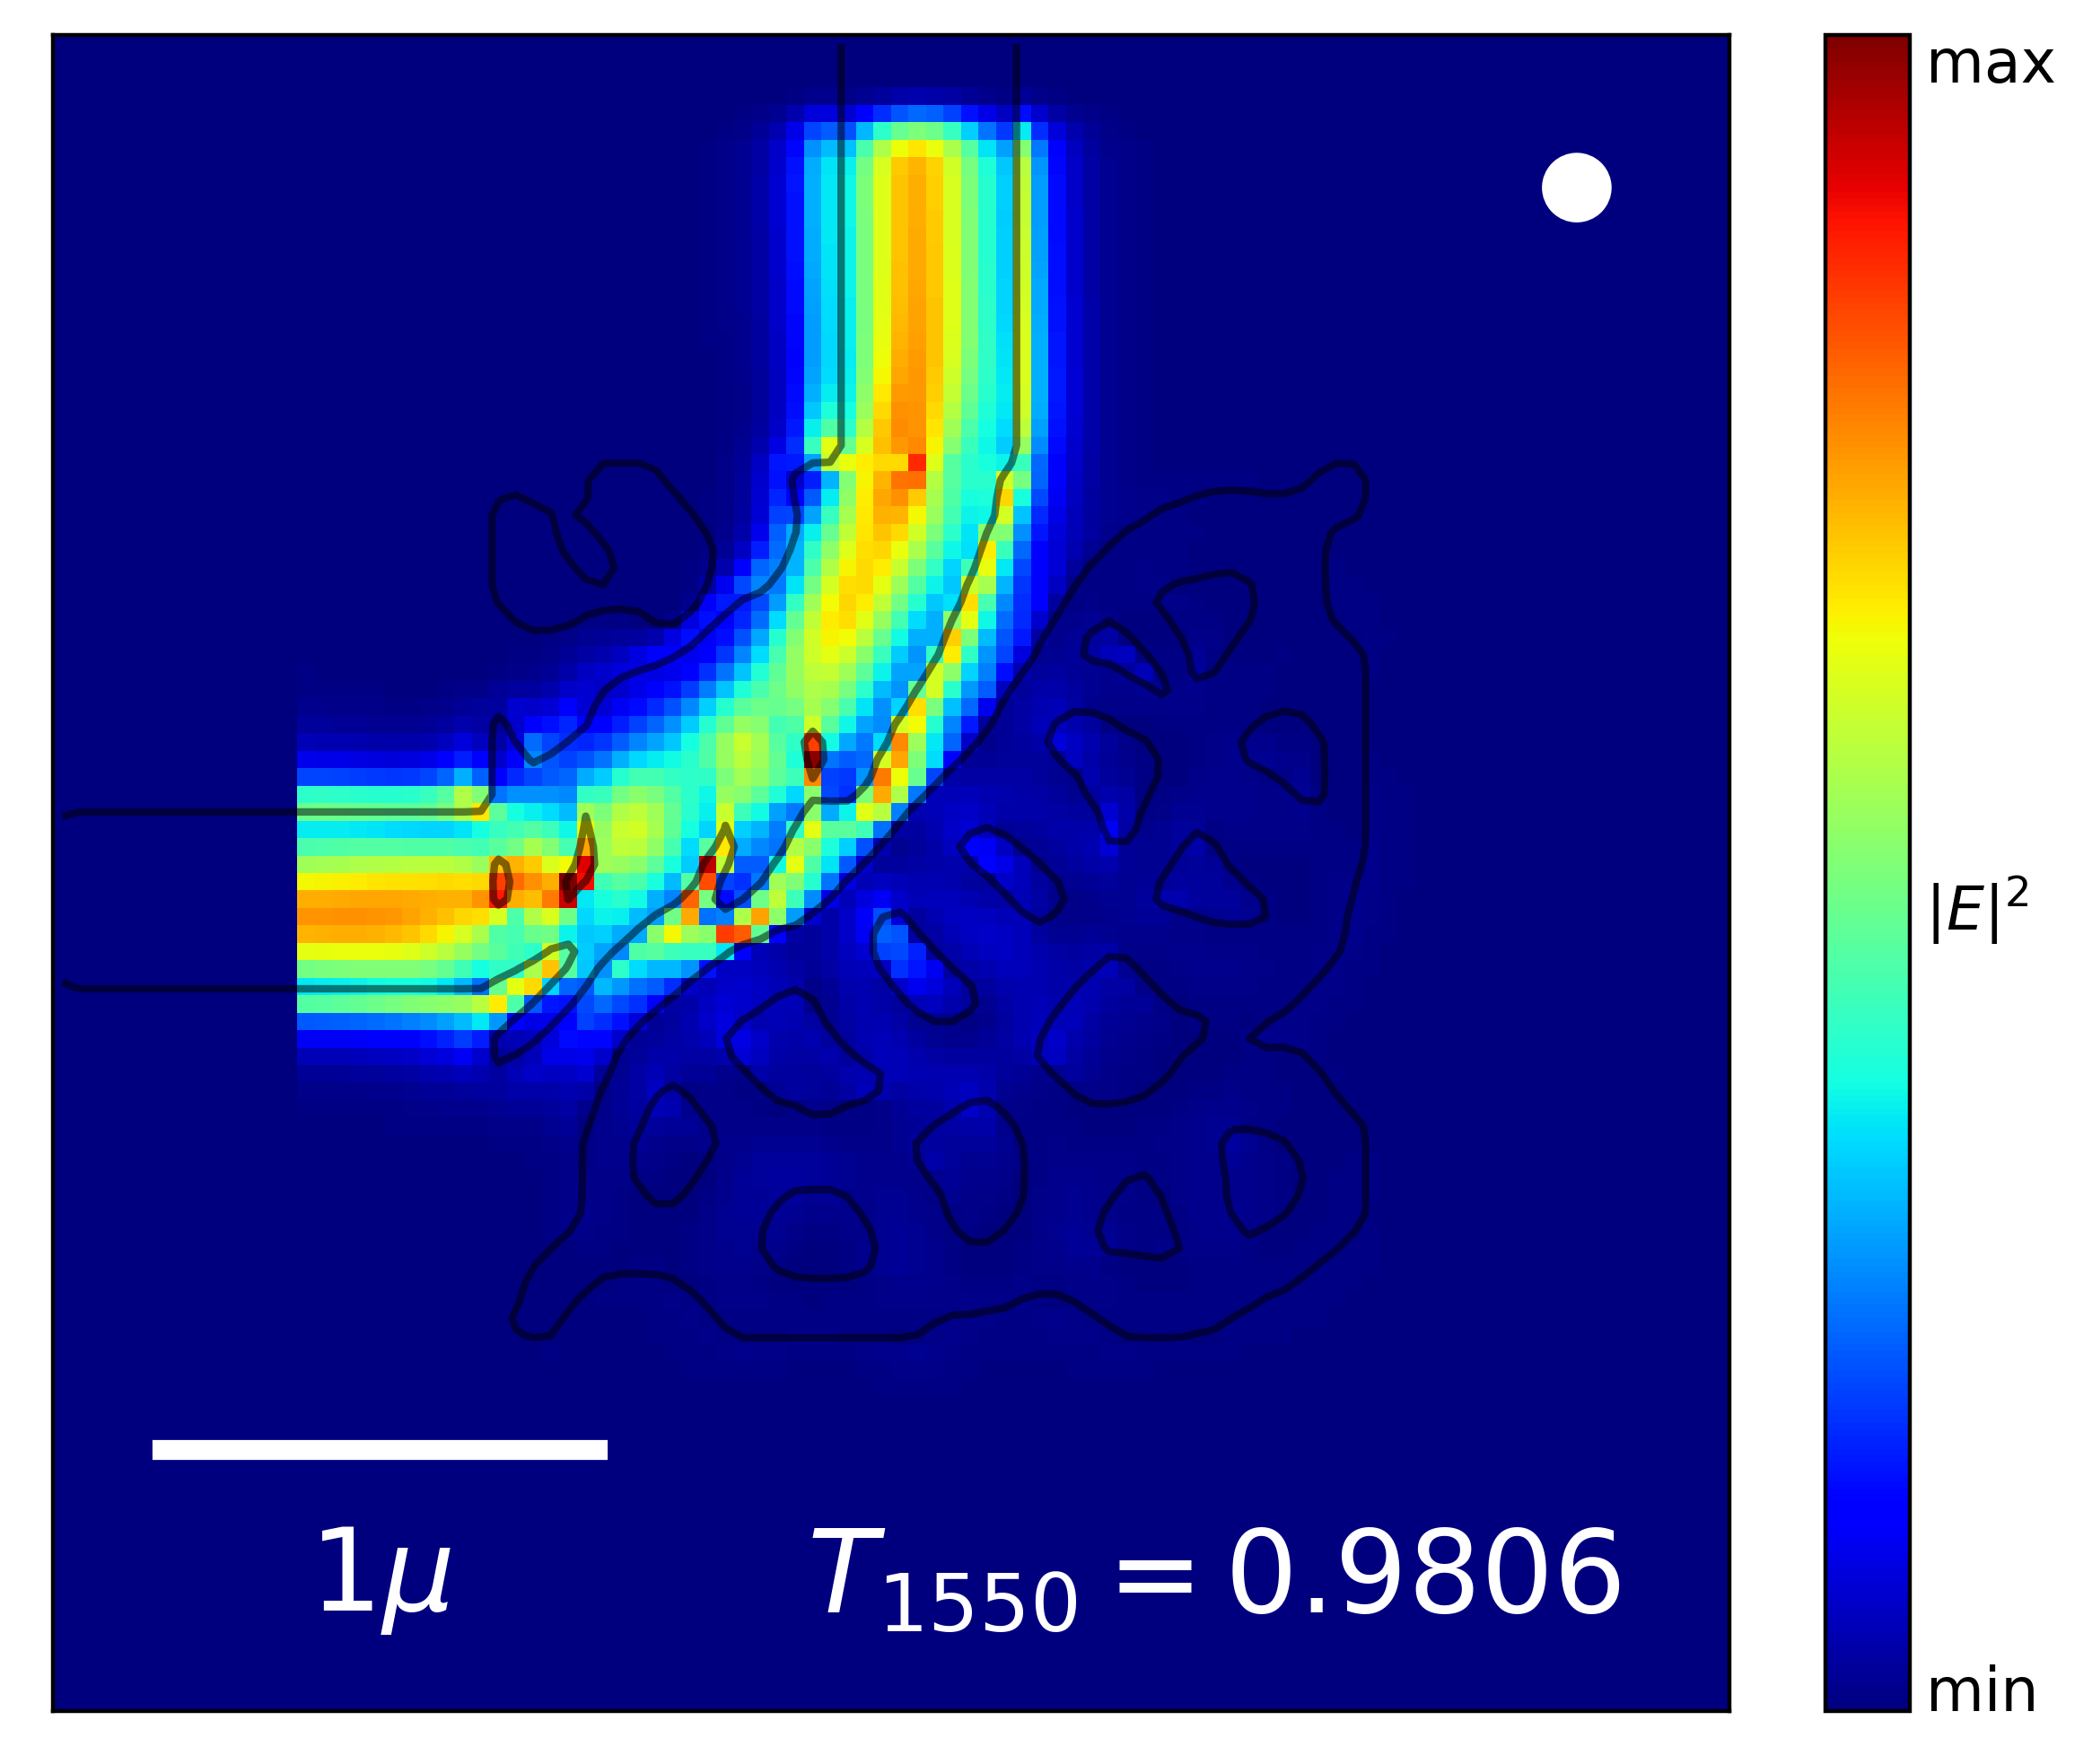
\includegraphics[width=0.33\textwidth]{image/results/bend/L-BFGS-B/visualize_field_disc_128.png} &
      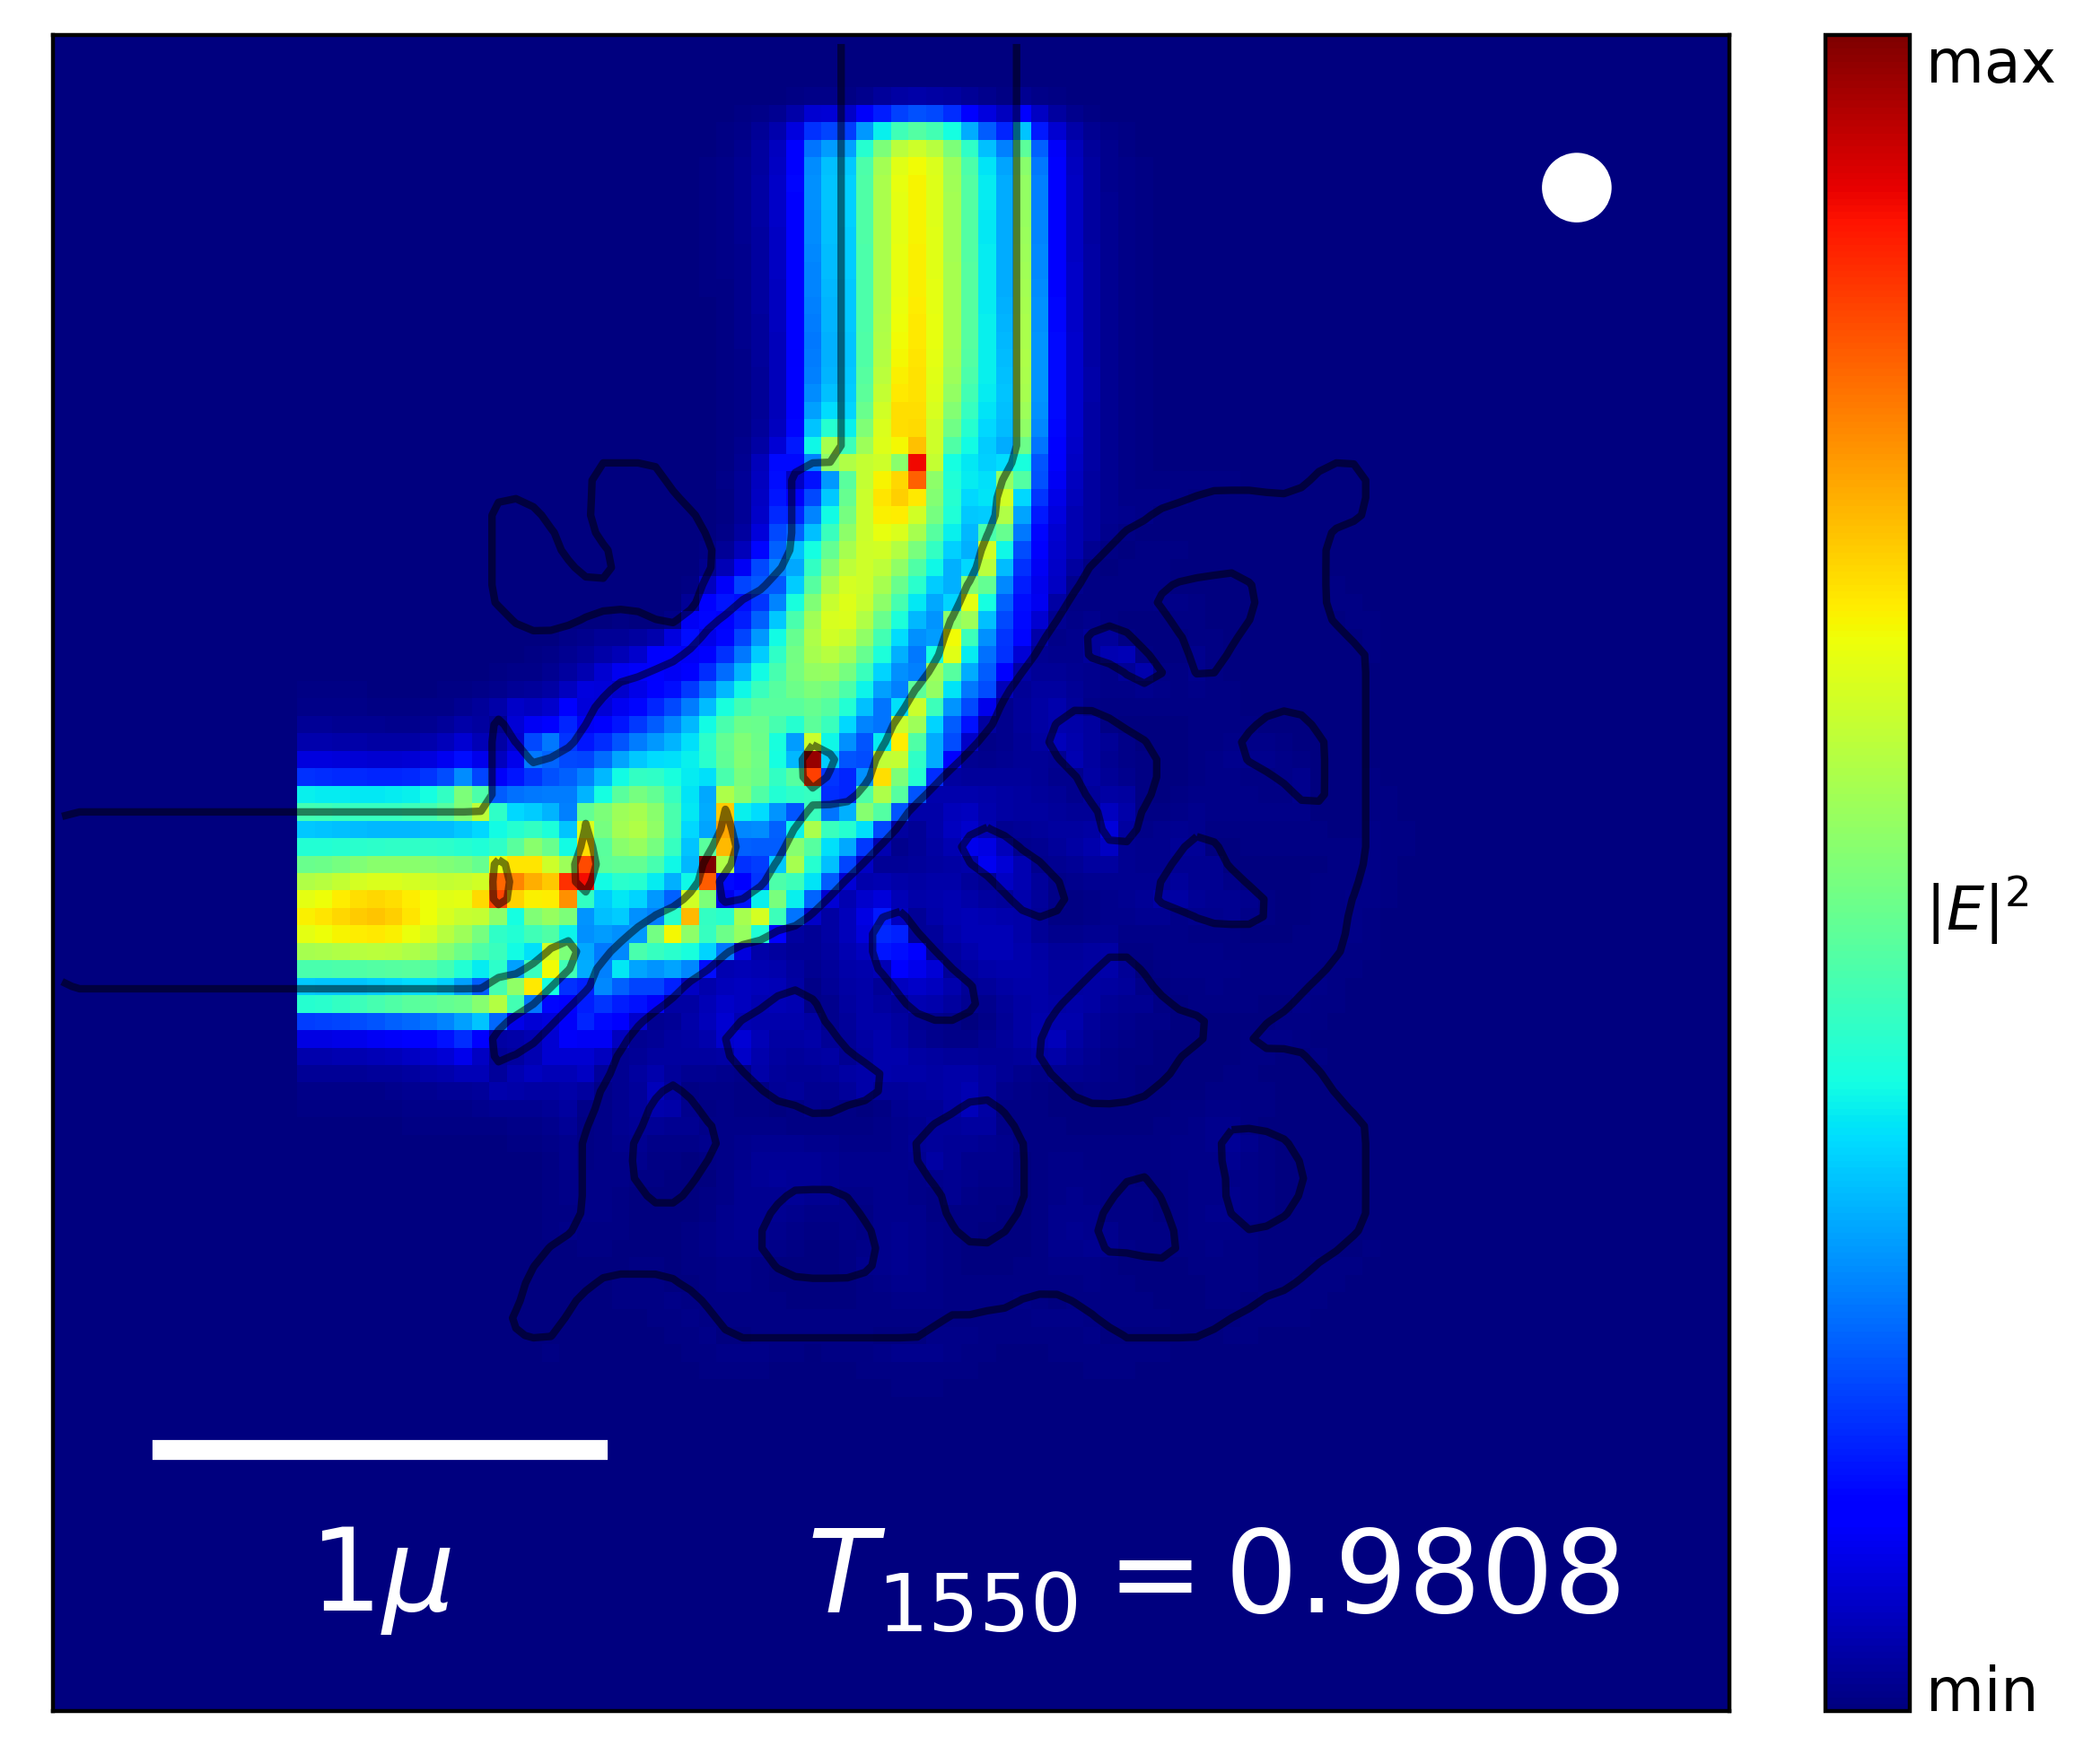
\includegraphics[width=0.33\textwidth]{image/results/bend/L-BFGS-B/visualize_field_fab_128.png} \\
    \hline
      \multirow{2}{*}{256} &
      
\includegraphics[width=0.20\textwidth]{image/results/bend/L-BFGS-B/visualize_eps_cont_256.png} &
      
\includegraphics[width=0.20\textwidth]{image/results/bend/L-BFGS-B/visualize_eps_disc_256.png} &
      
\includegraphics[width=0.20\textwidth]{image/results/bend/L-BFGS-B/visualize_eps_fab_256.png} \\
      \cline{2-4}
      &
      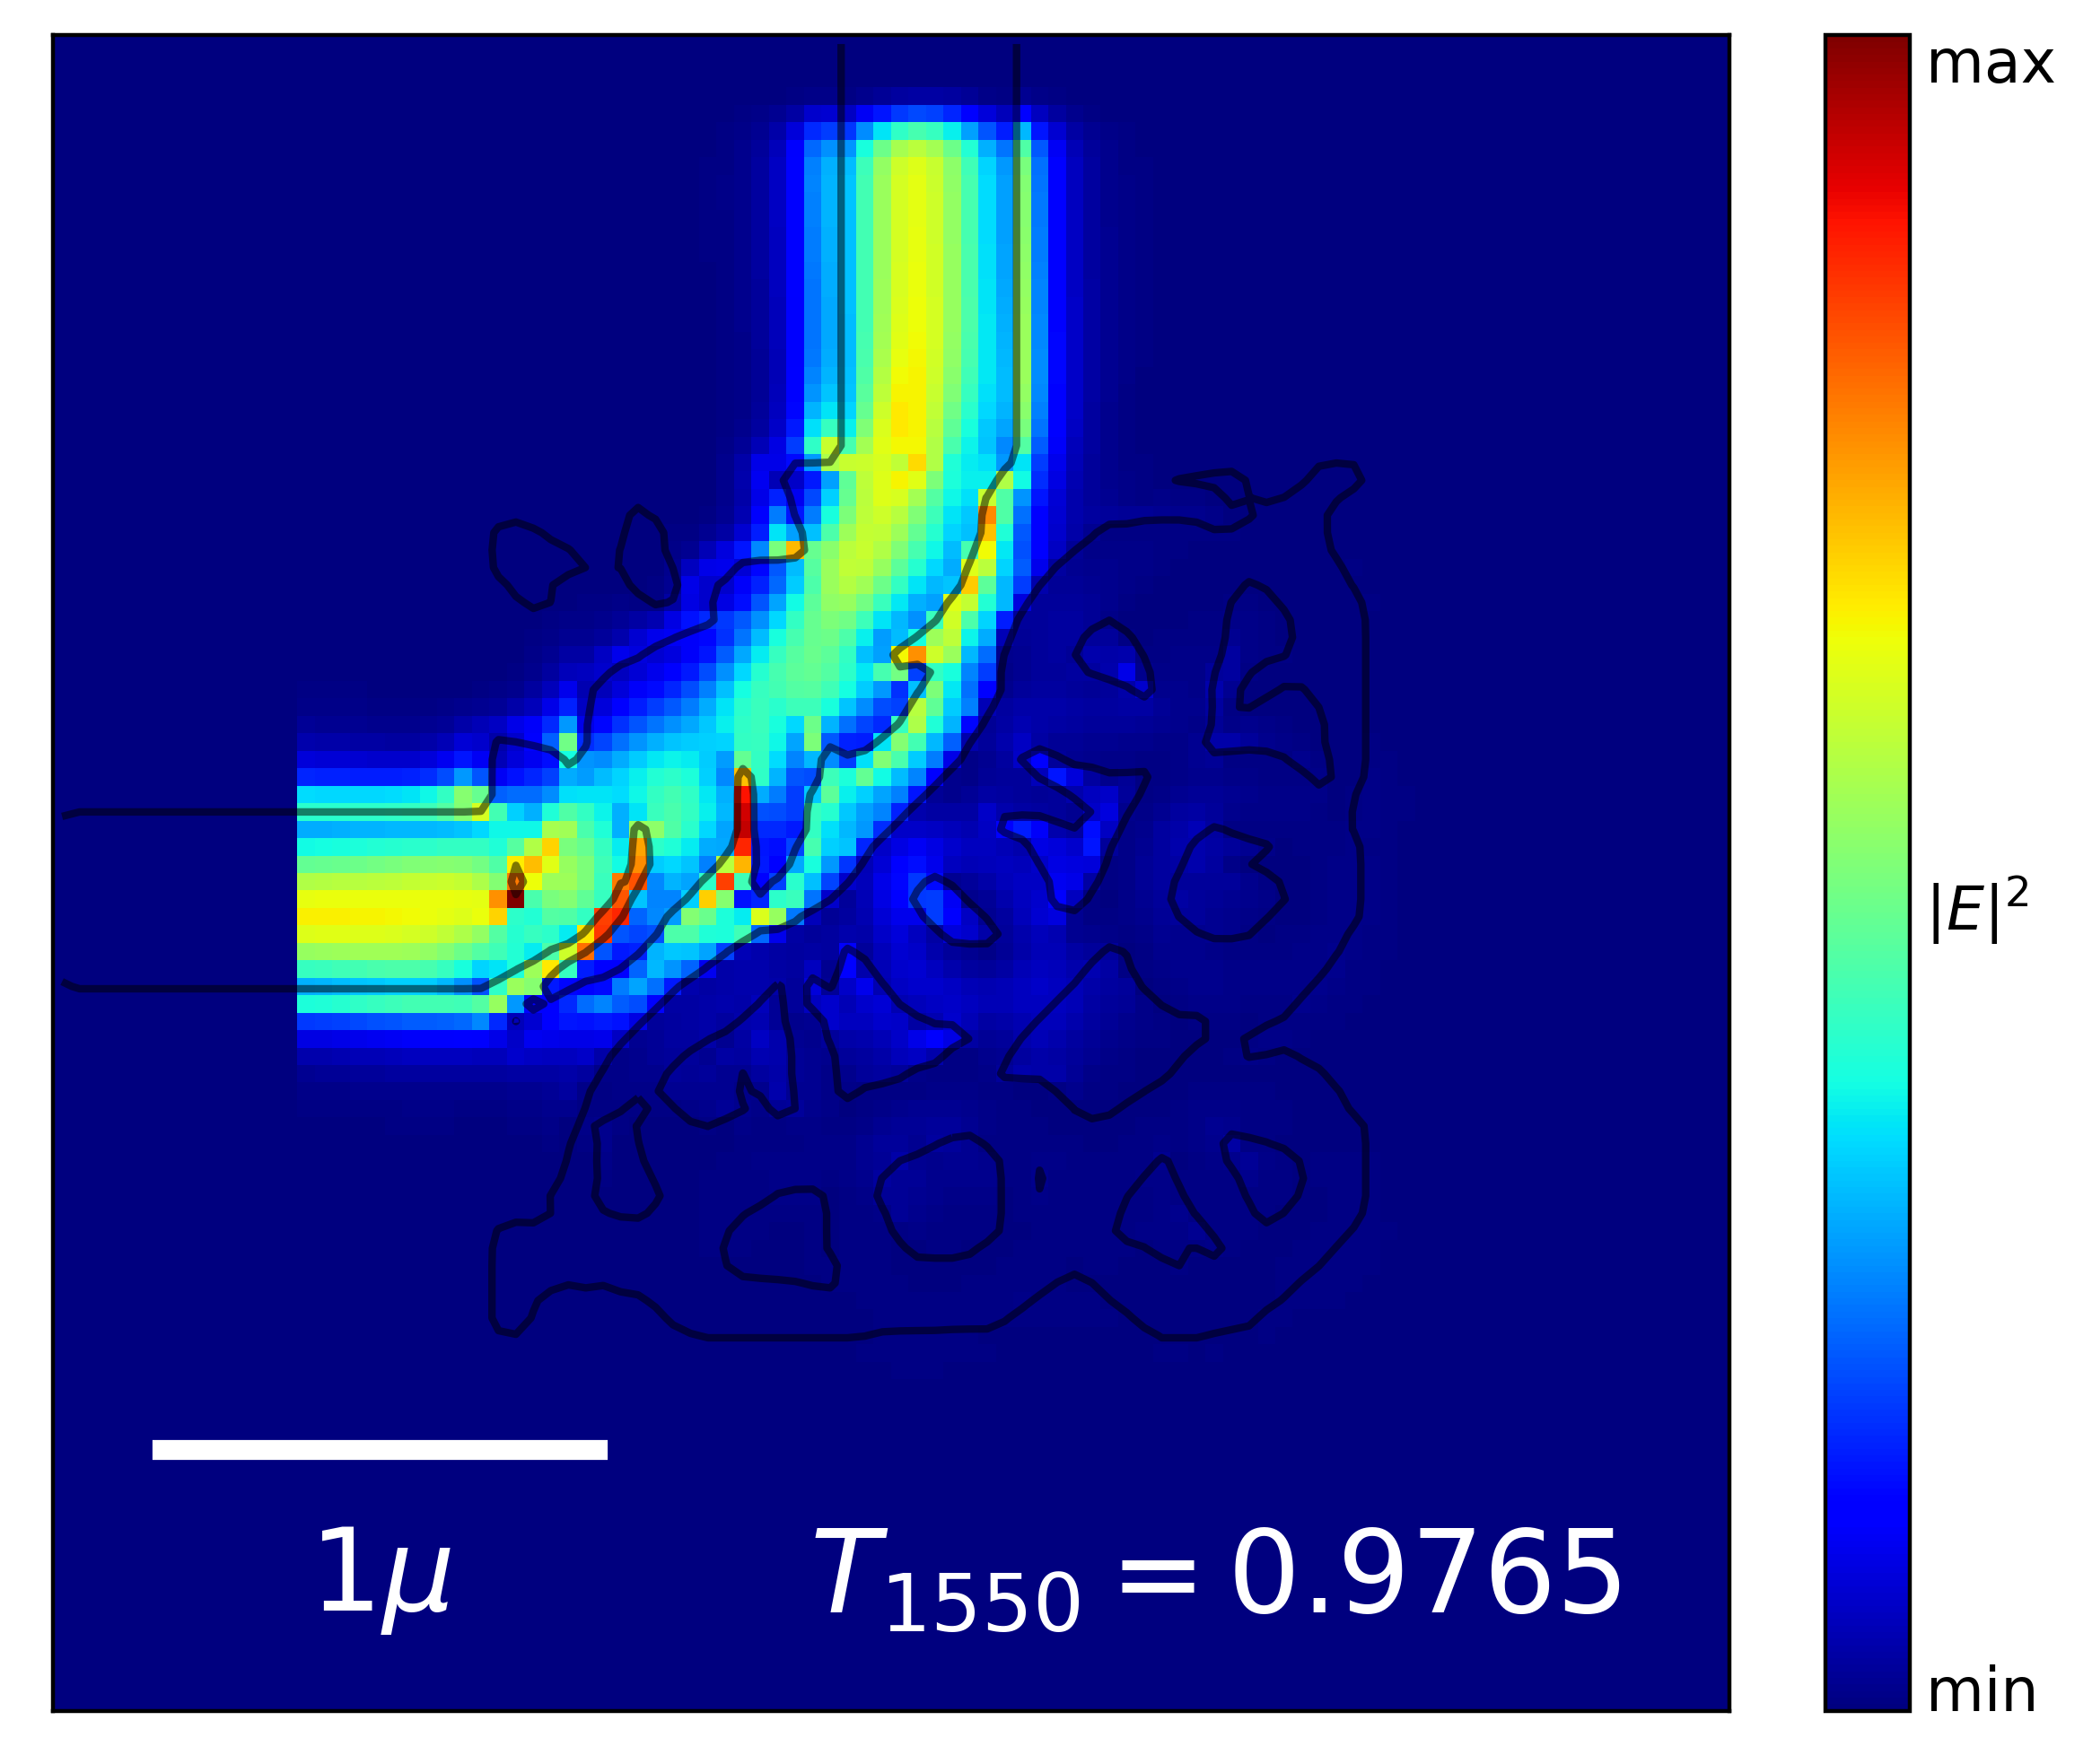
\includegraphics[width=0.33\textwidth]{image/results/bend/L-BFGS-B/visualize_field_cont_256.png} &
      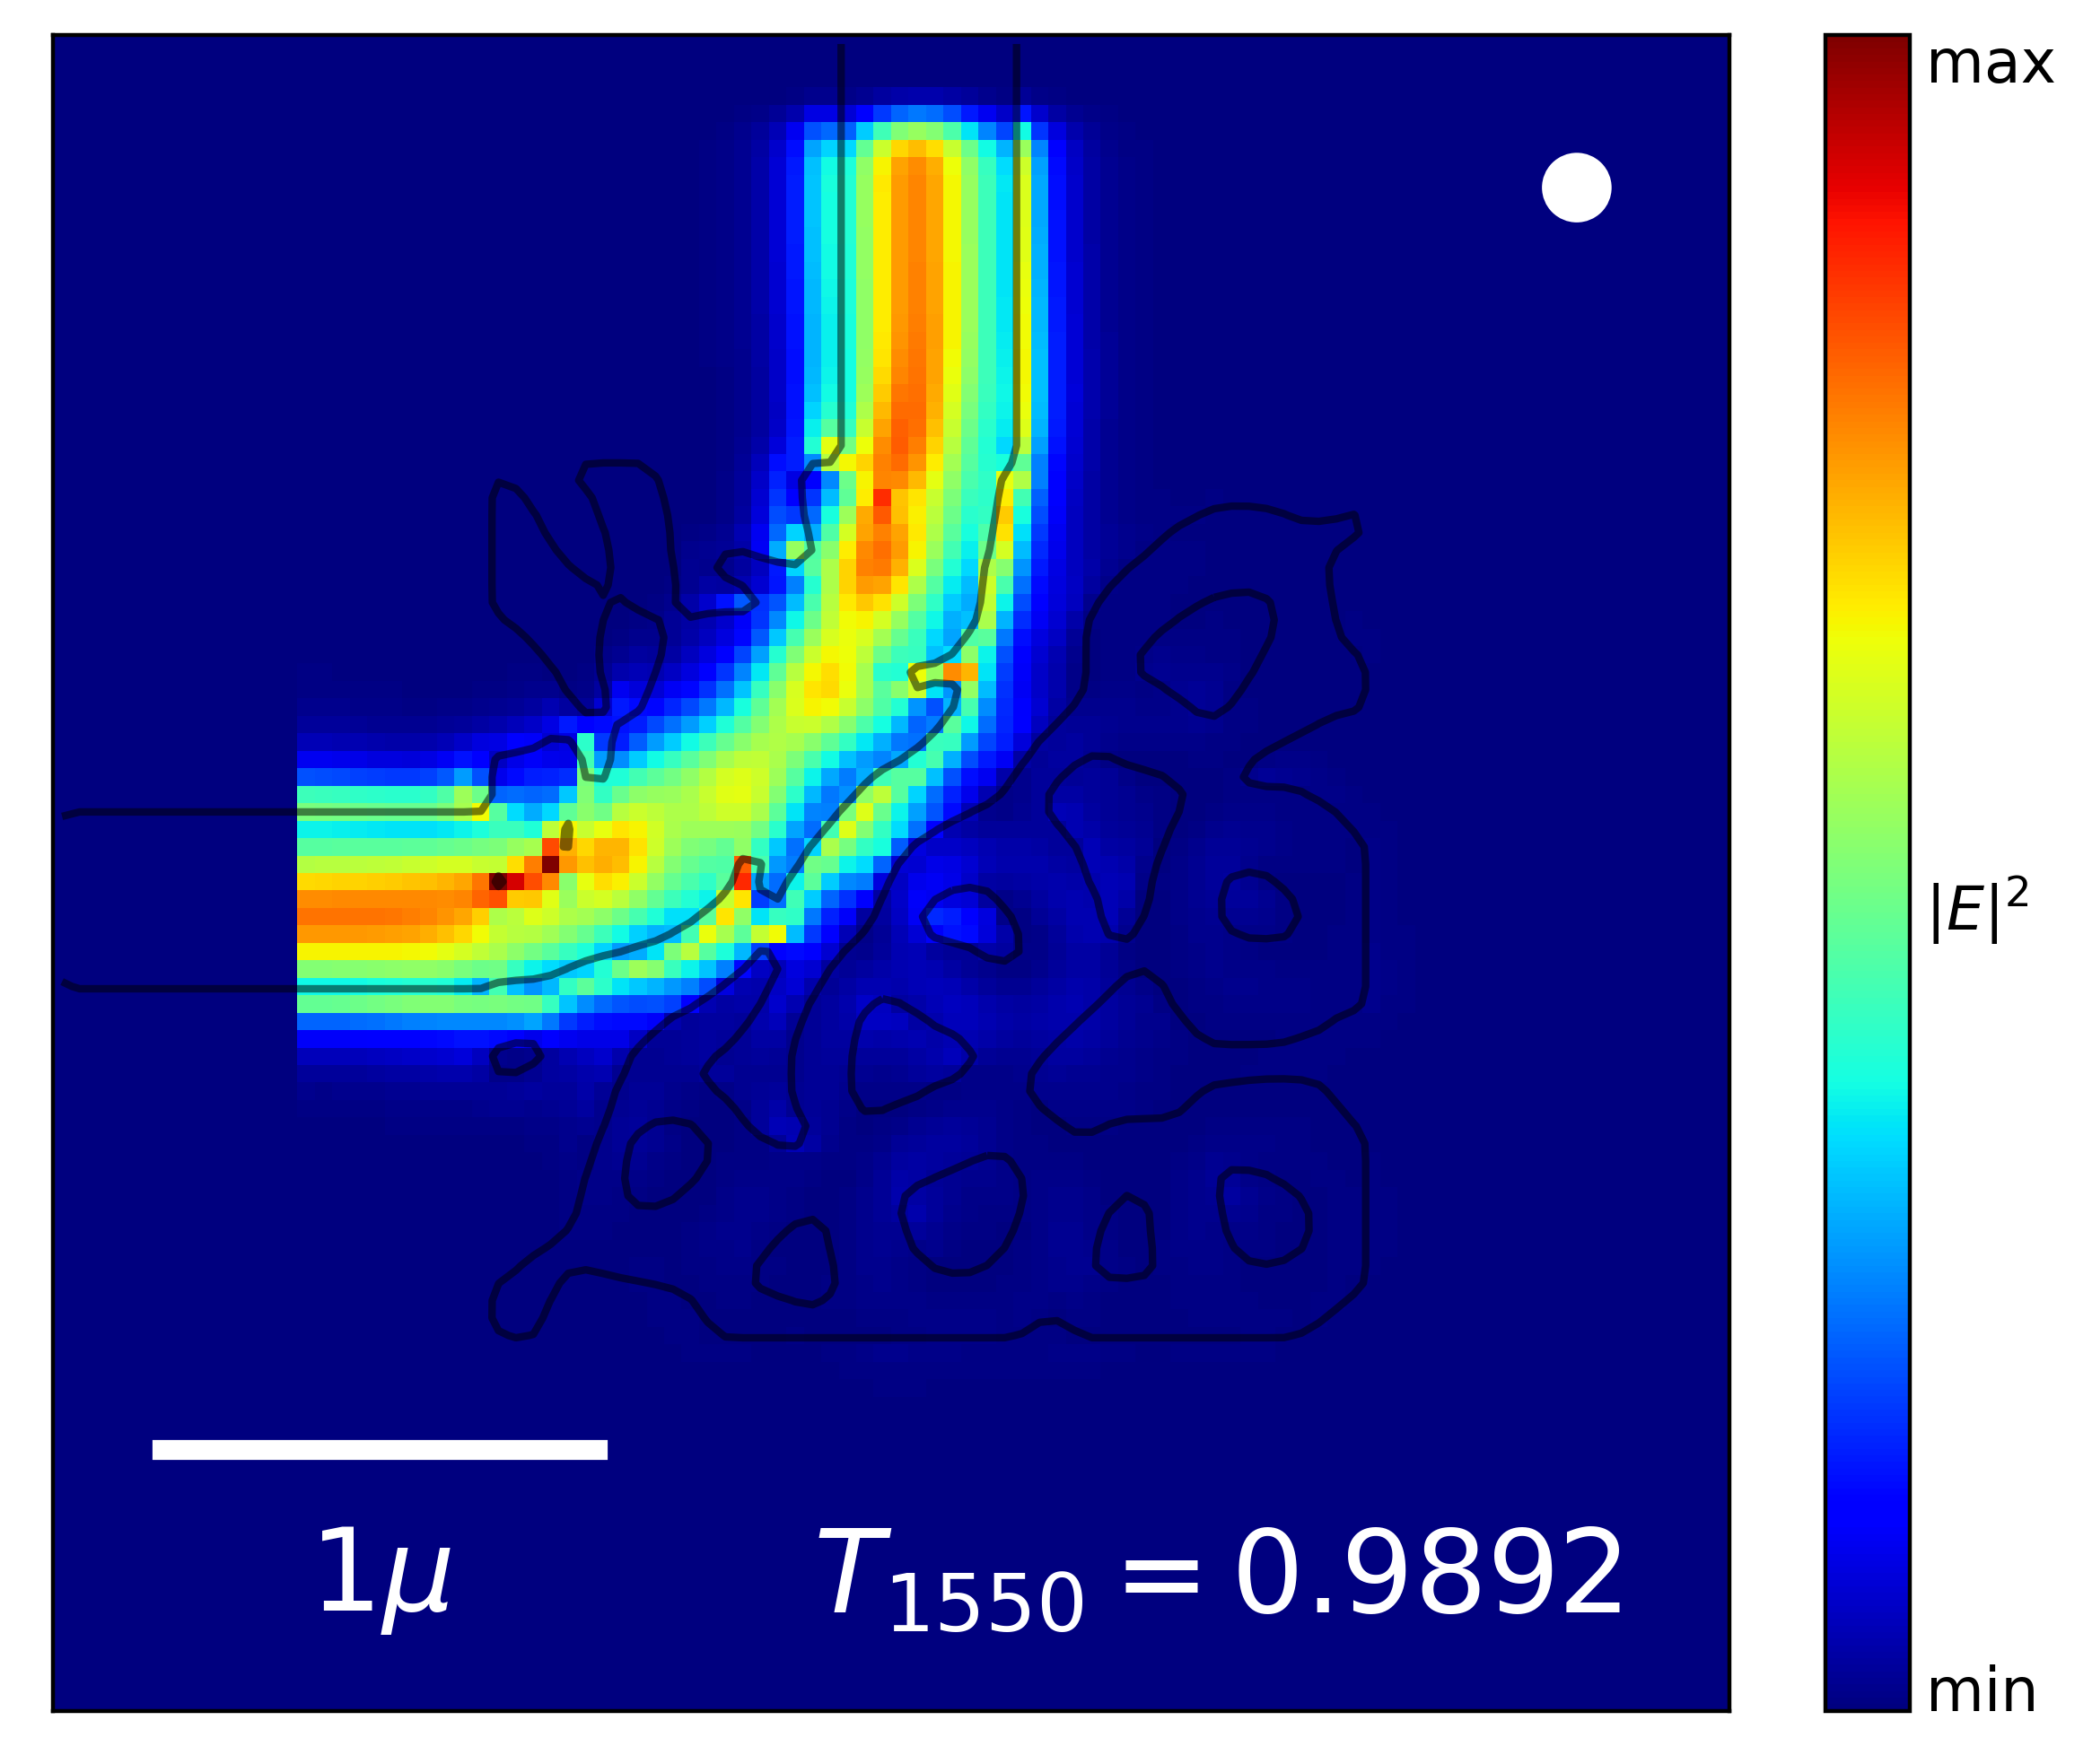
\includegraphics[width=0.33\textwidth]{image/results/bend/L-BFGS-B/visualize_field_disc_256.png} &
      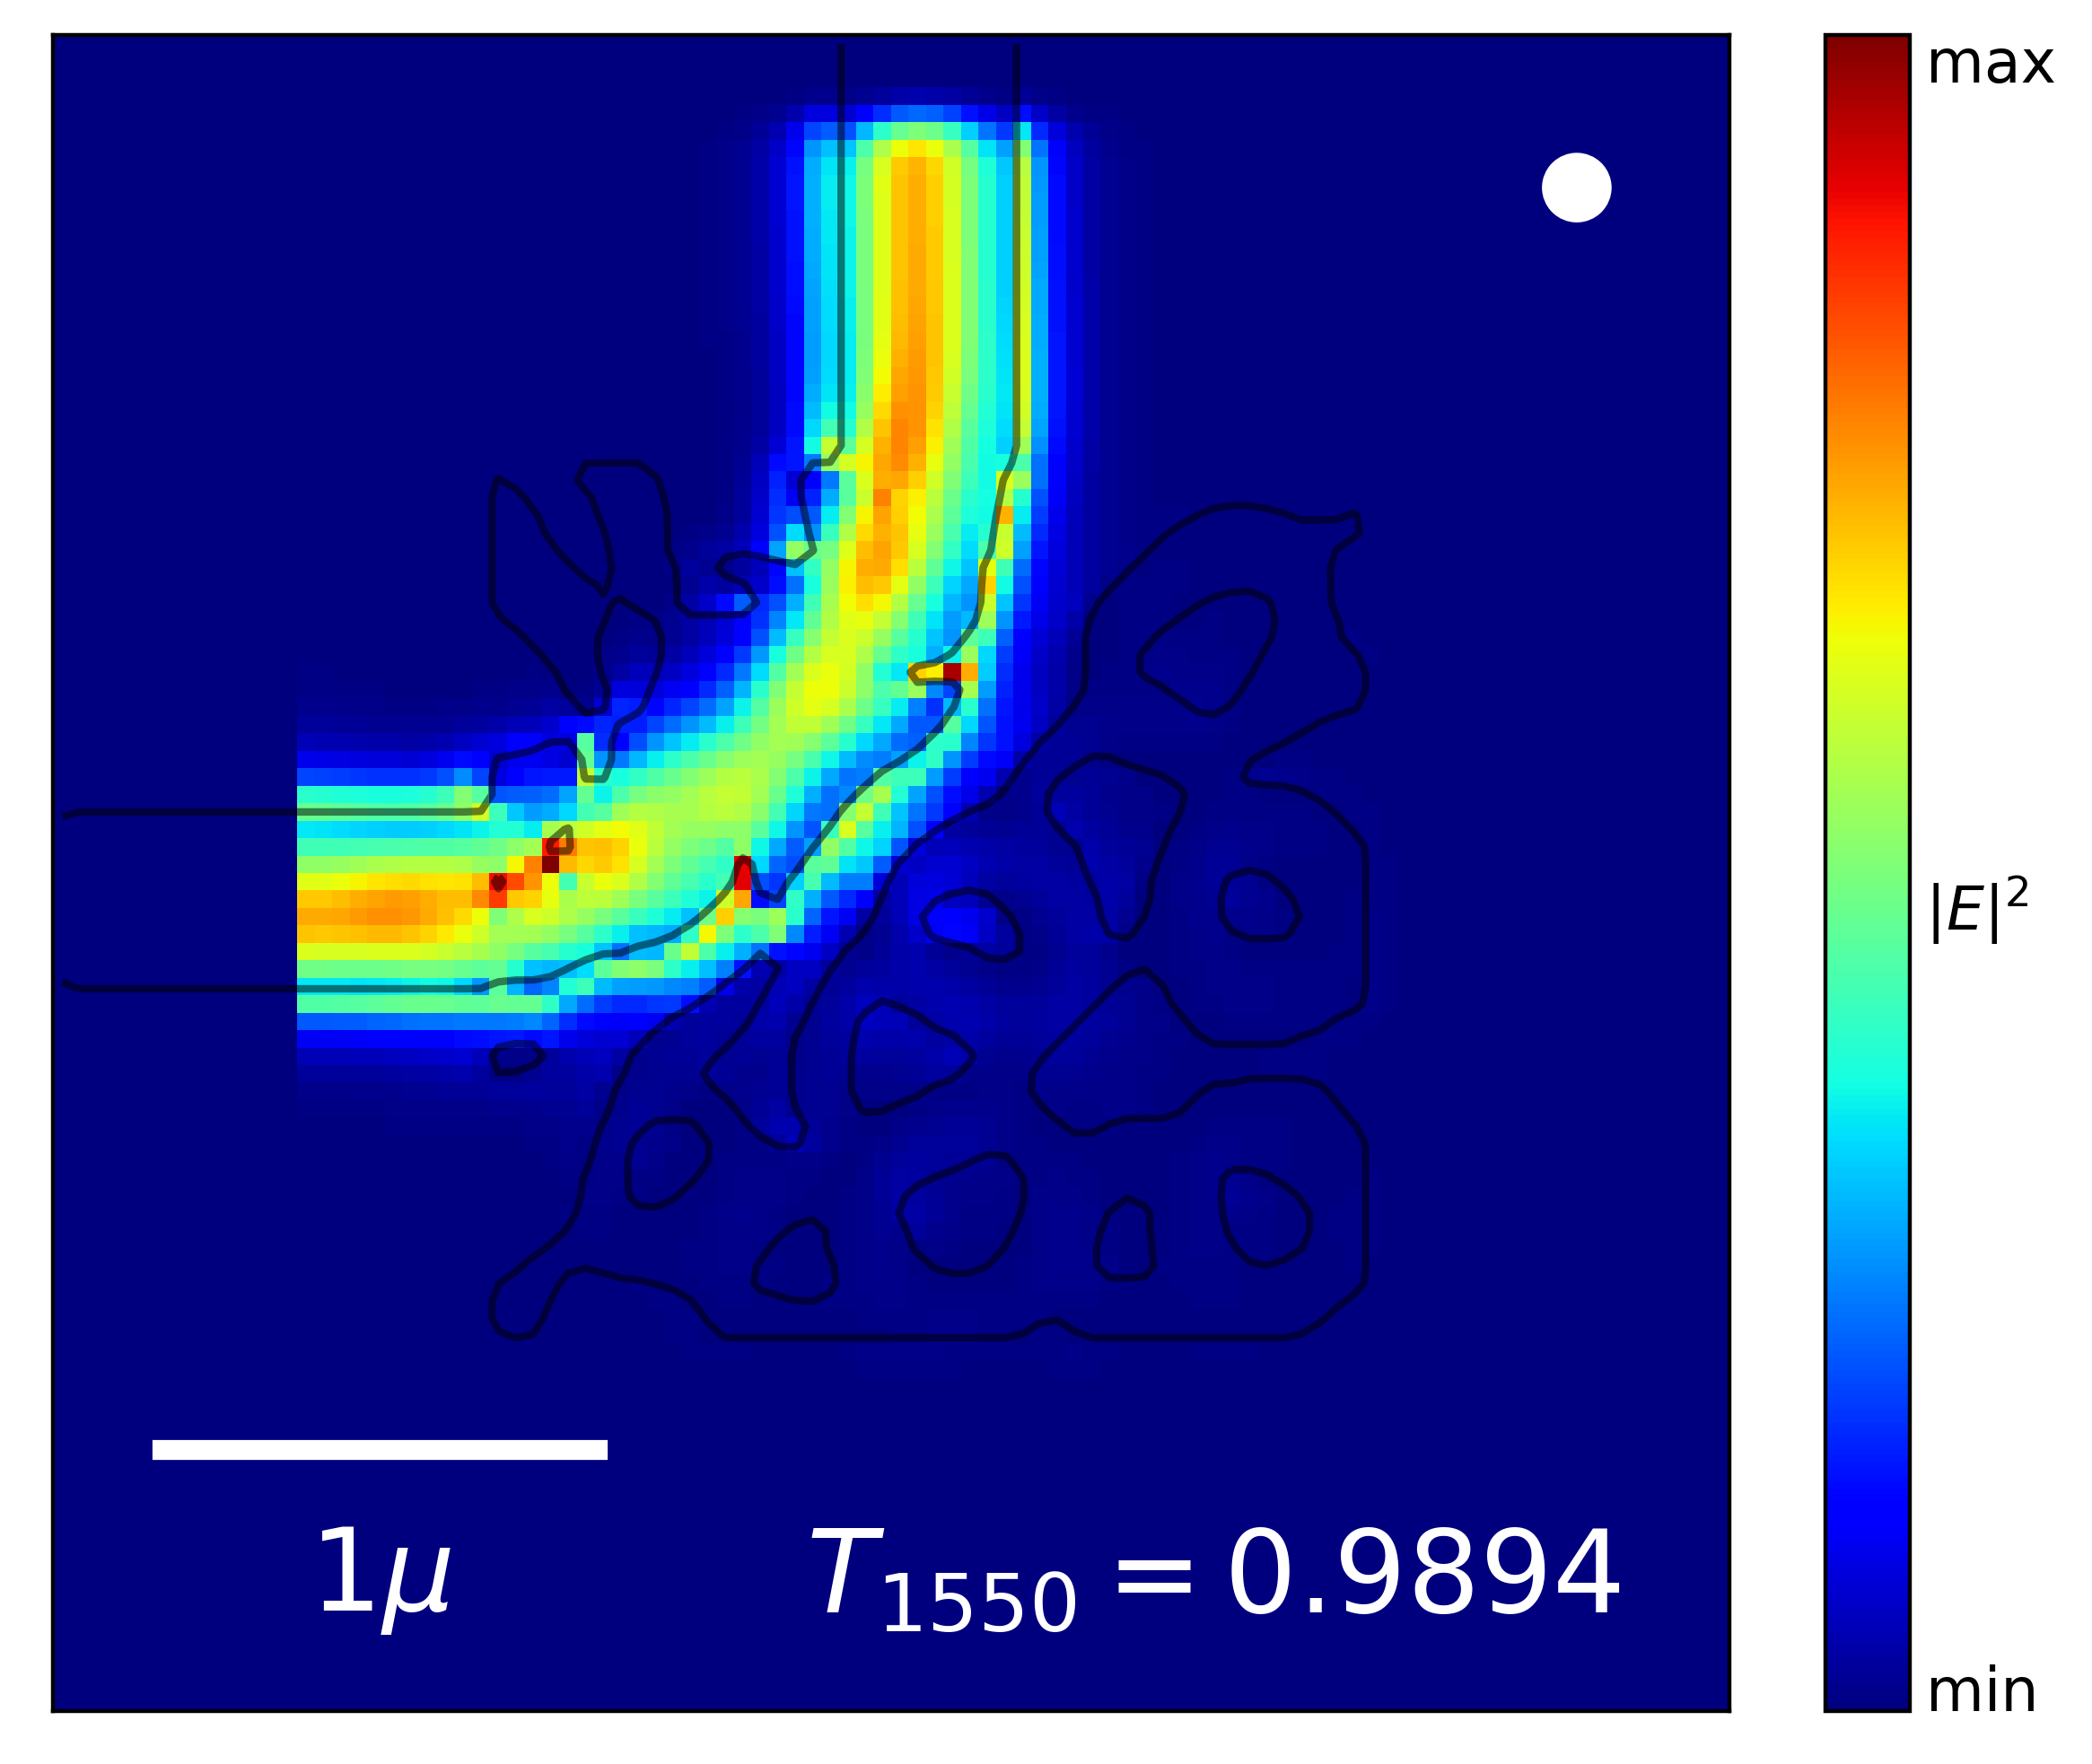
\includegraphics[width=0.33\textwidth]{image/results/bend/L-BFGS-B/visualize_field_fab_256.png} \\
    \hline
      \multirow{2}{*}{512} &
      
\includegraphics[width=0.20\textwidth]{image/results/bend/L-BFGS-B/visualize_eps_cont_512.png} &
      
\includegraphics[width=0.20\textwidth]{image/results/bend/L-BFGS-B/visualize_eps_disc_512.png} &
      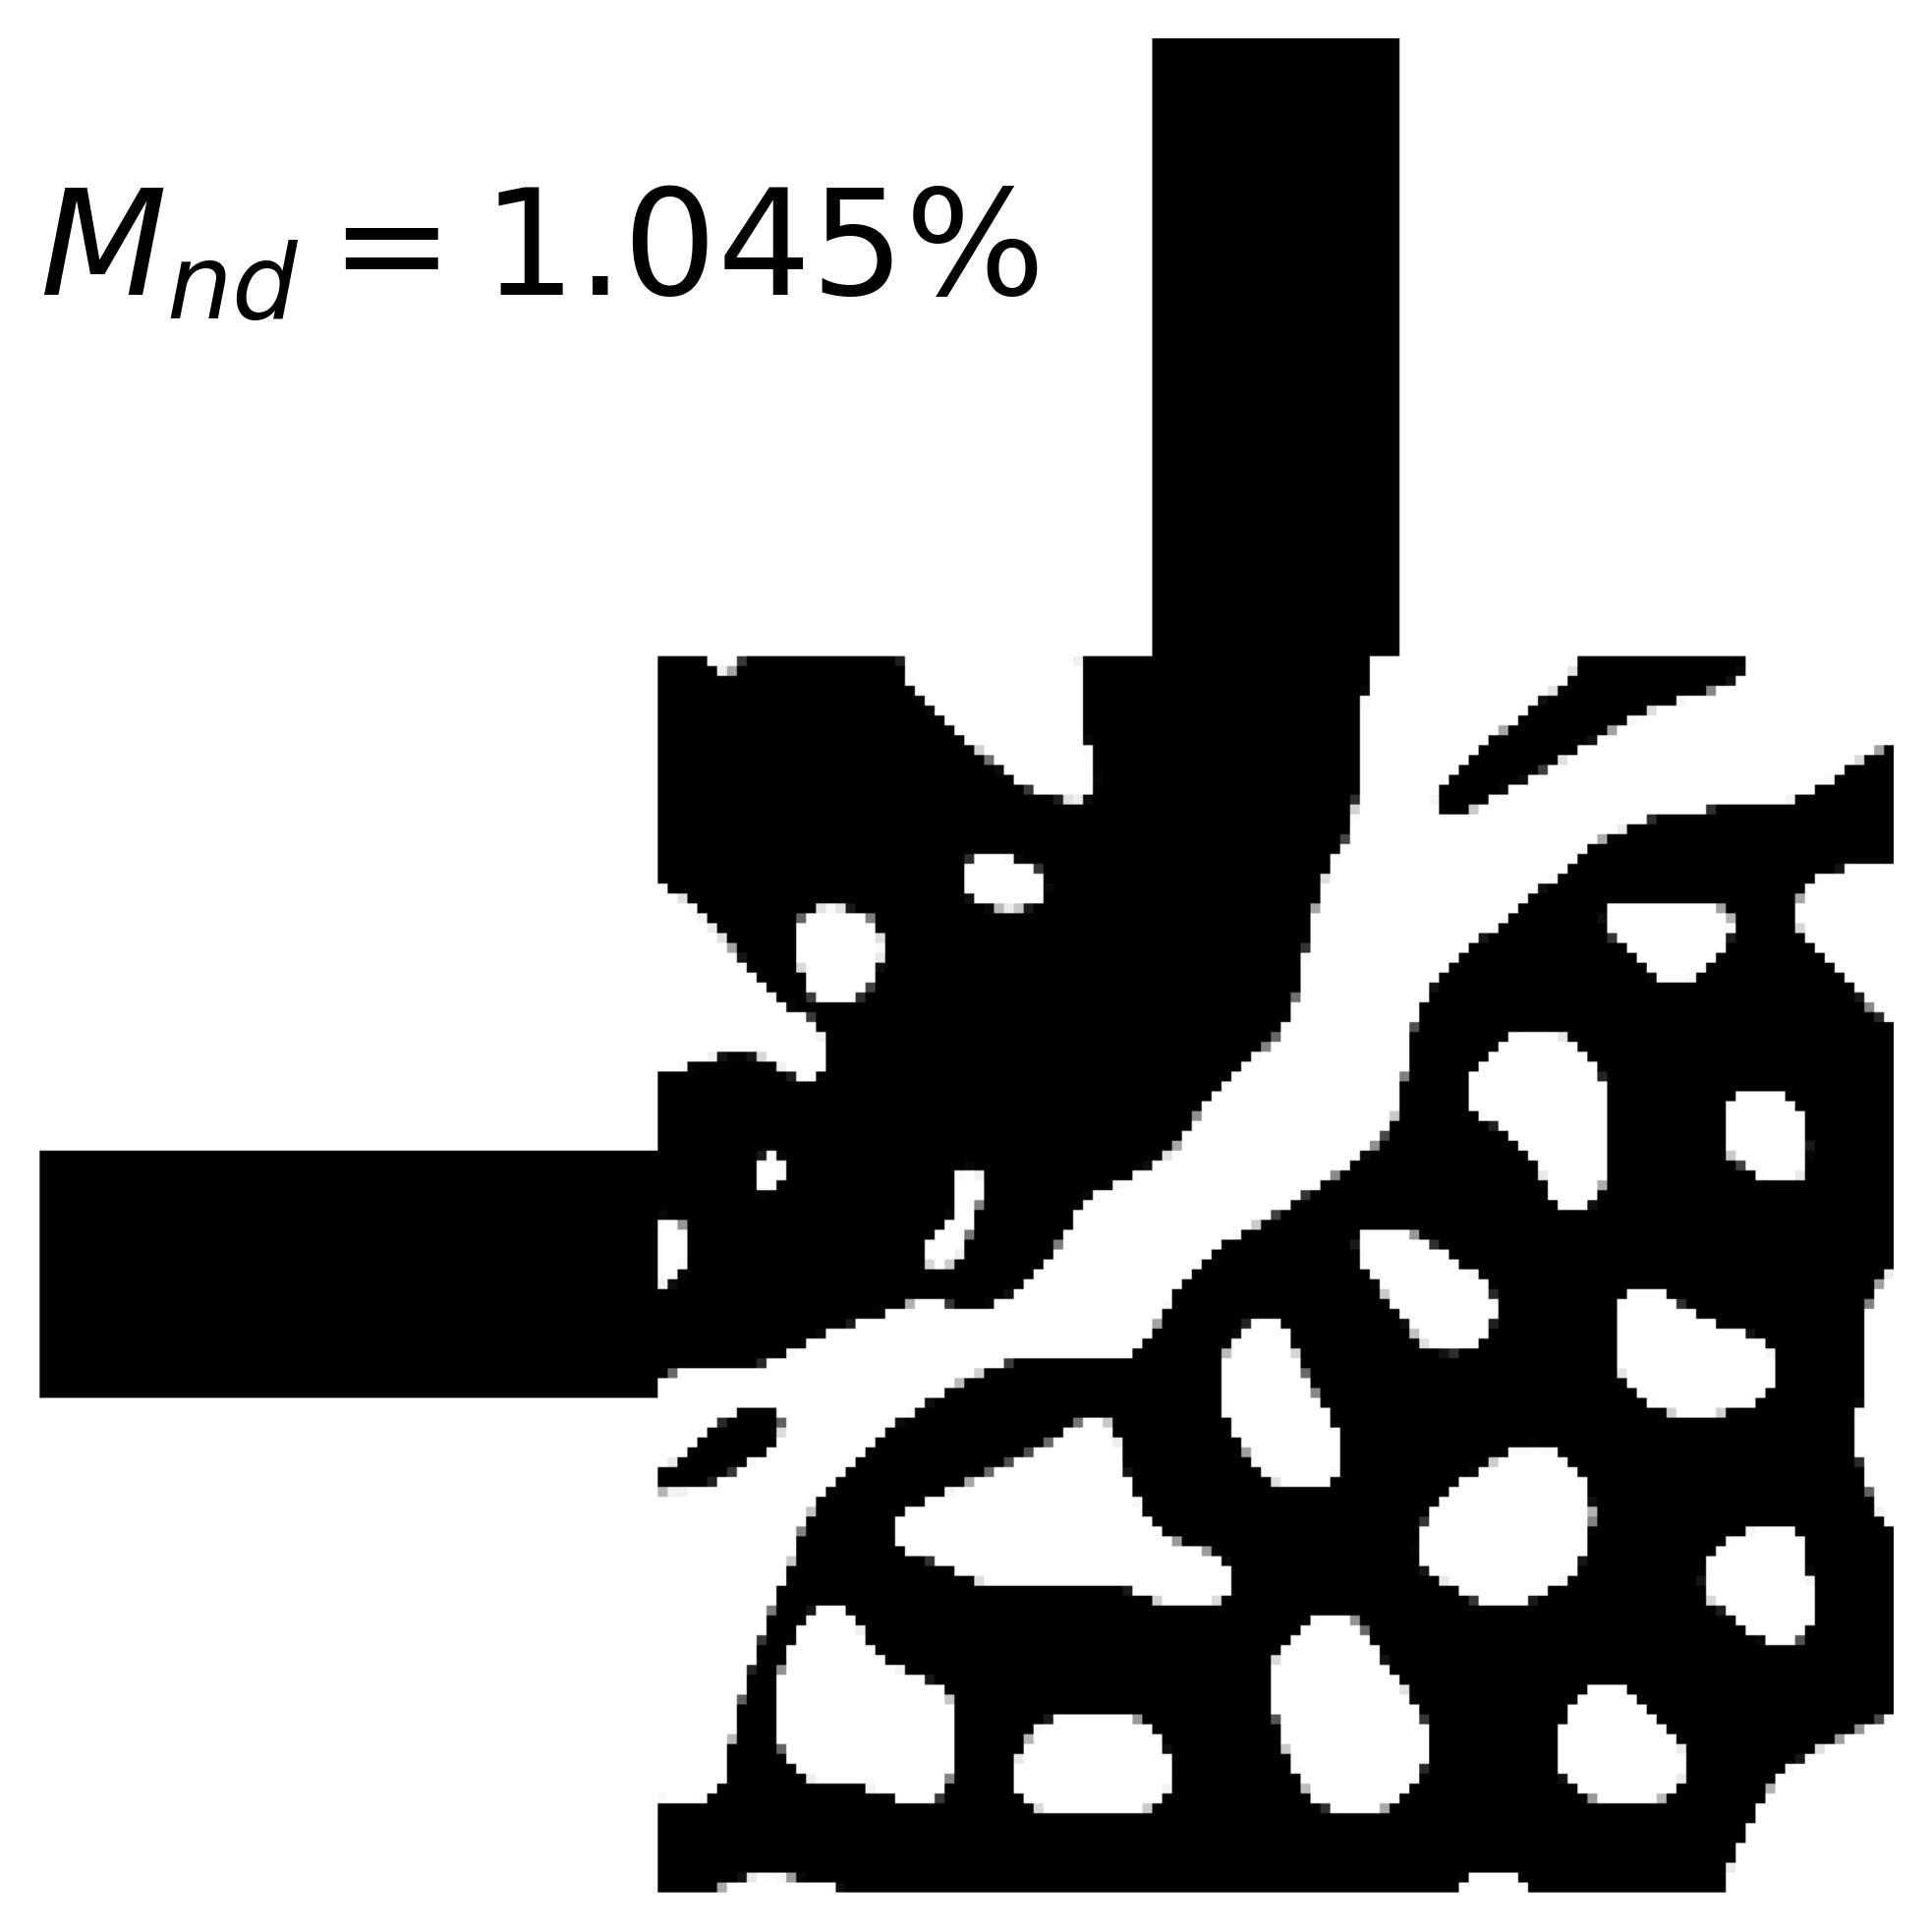
\includegraphics[width=0.20\textwidth]{image/results/bend/L-BFGS-B/visualize_eps_fab_512.png} \\
      \cline{2-4}
      &
      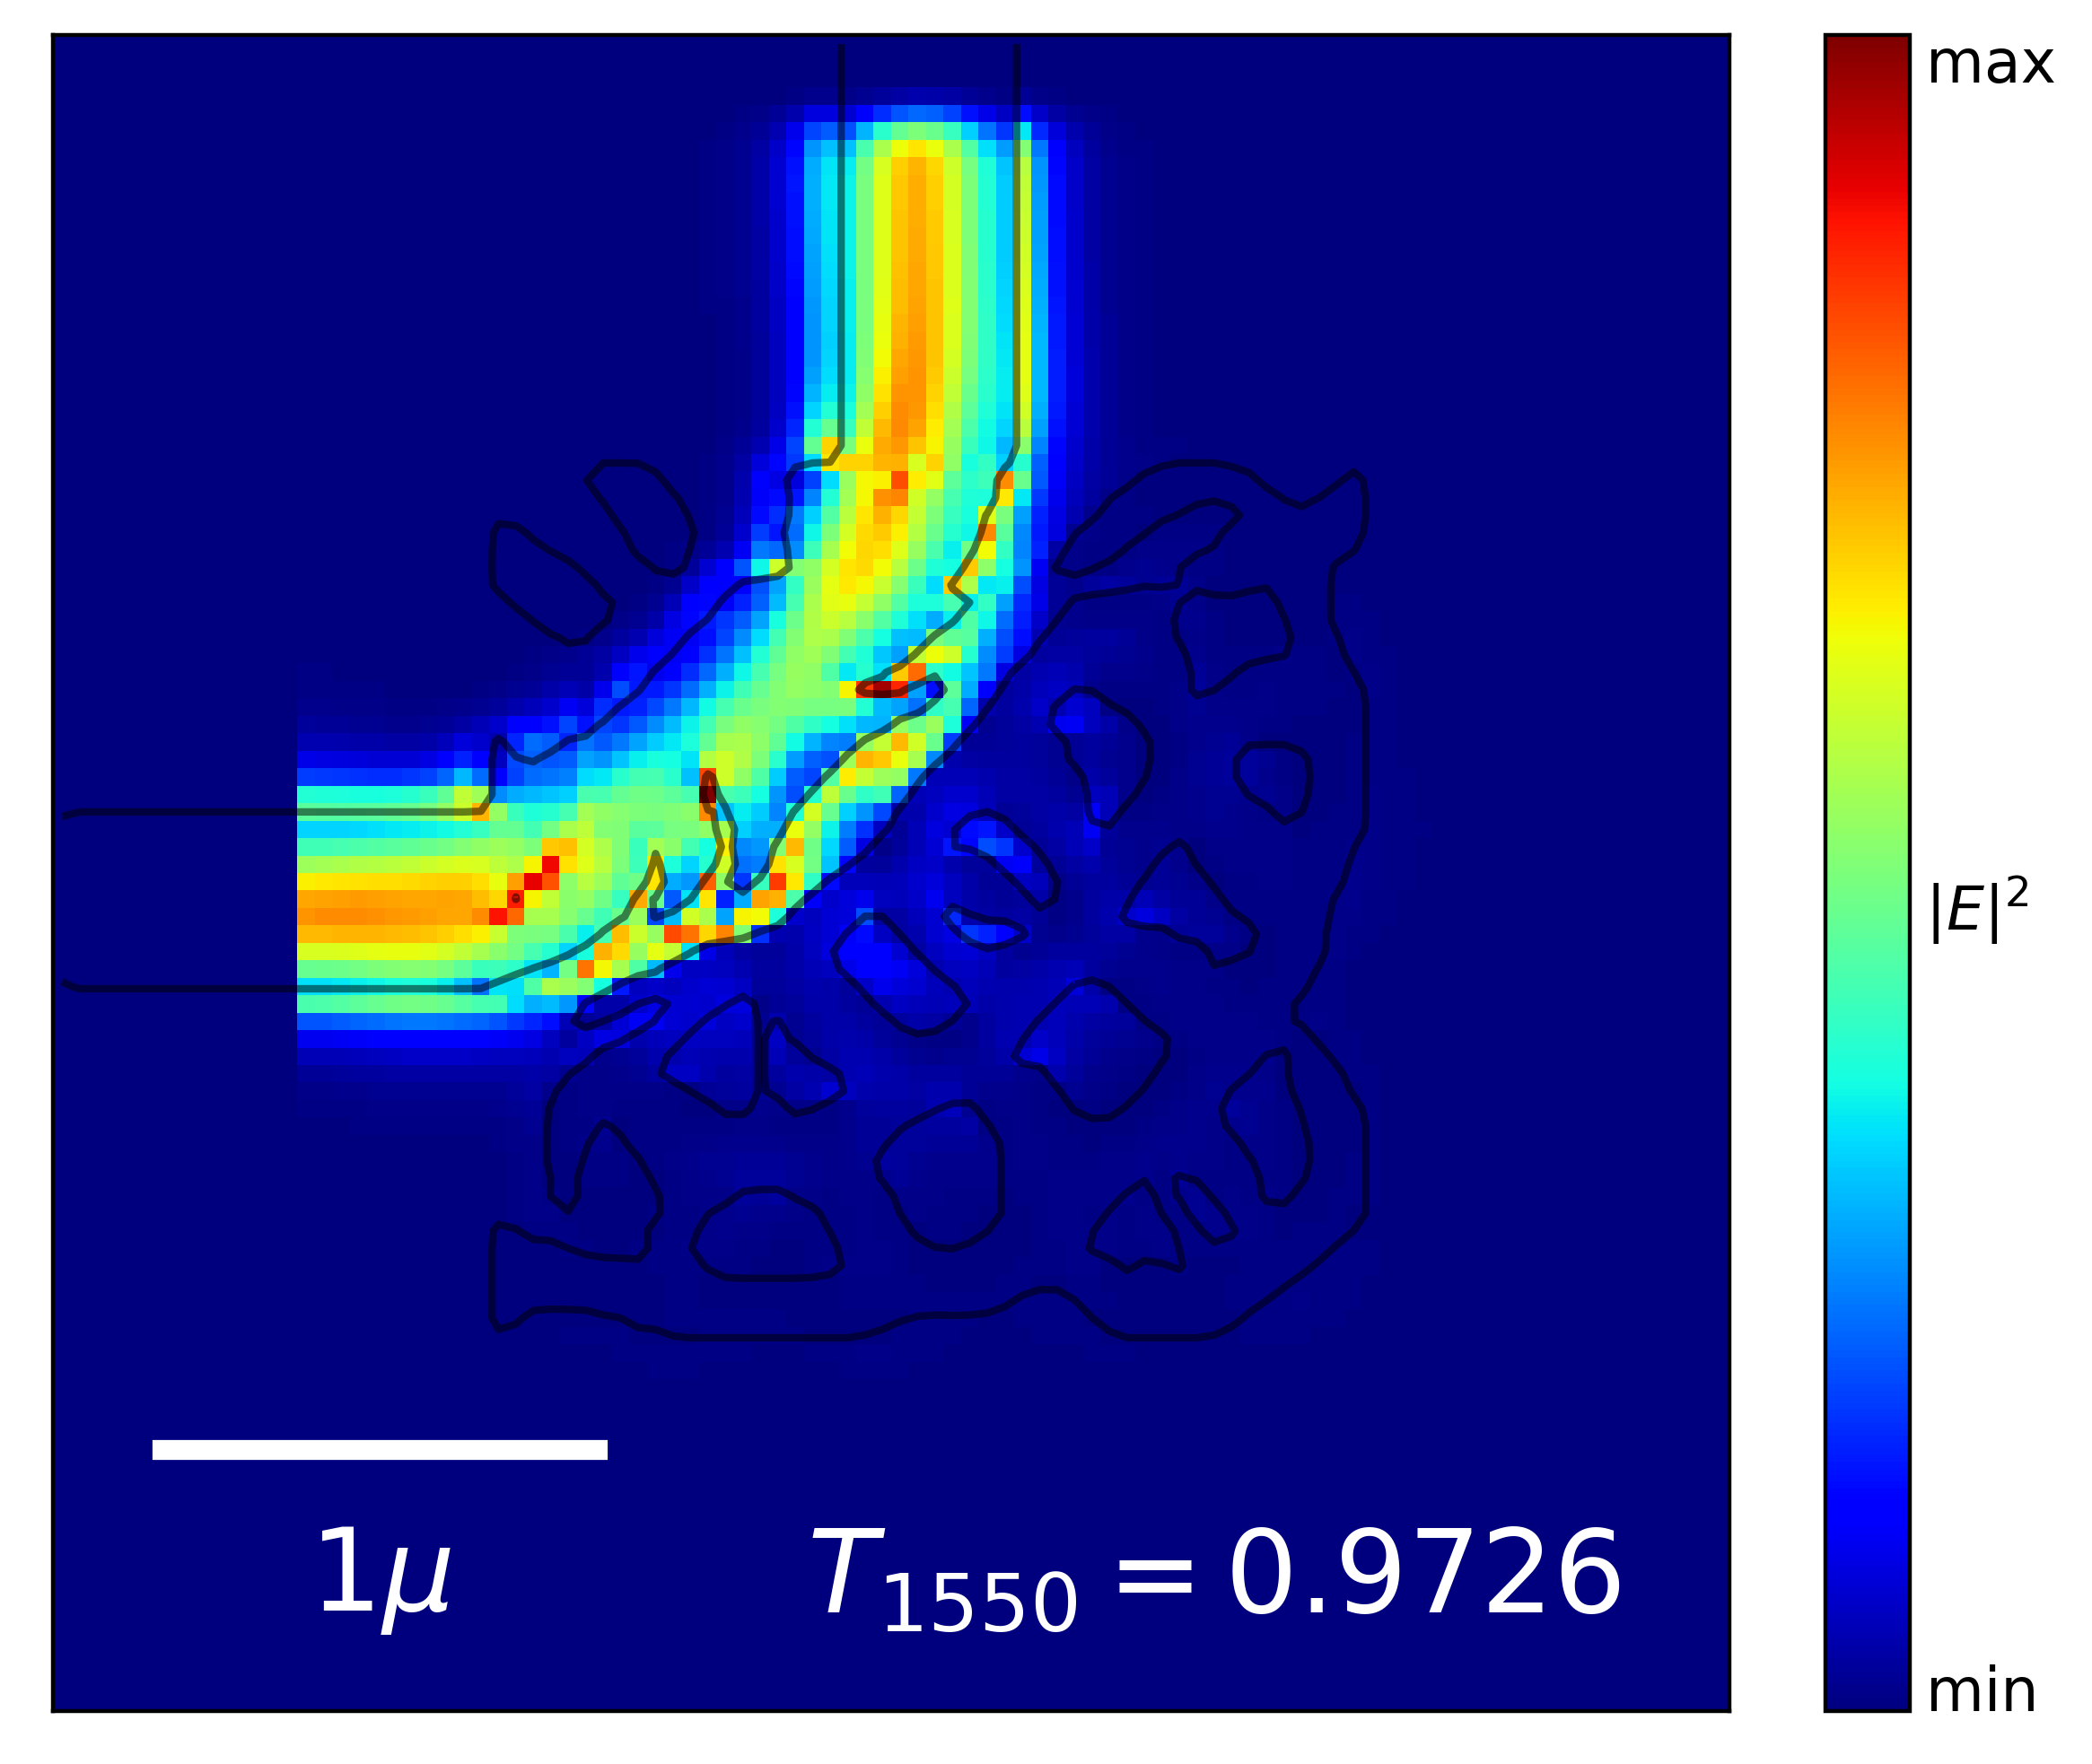
\includegraphics[width=0.33\textwidth]{image/results/bend/L-BFGS-B/visualize_field_cont_512.png} &
      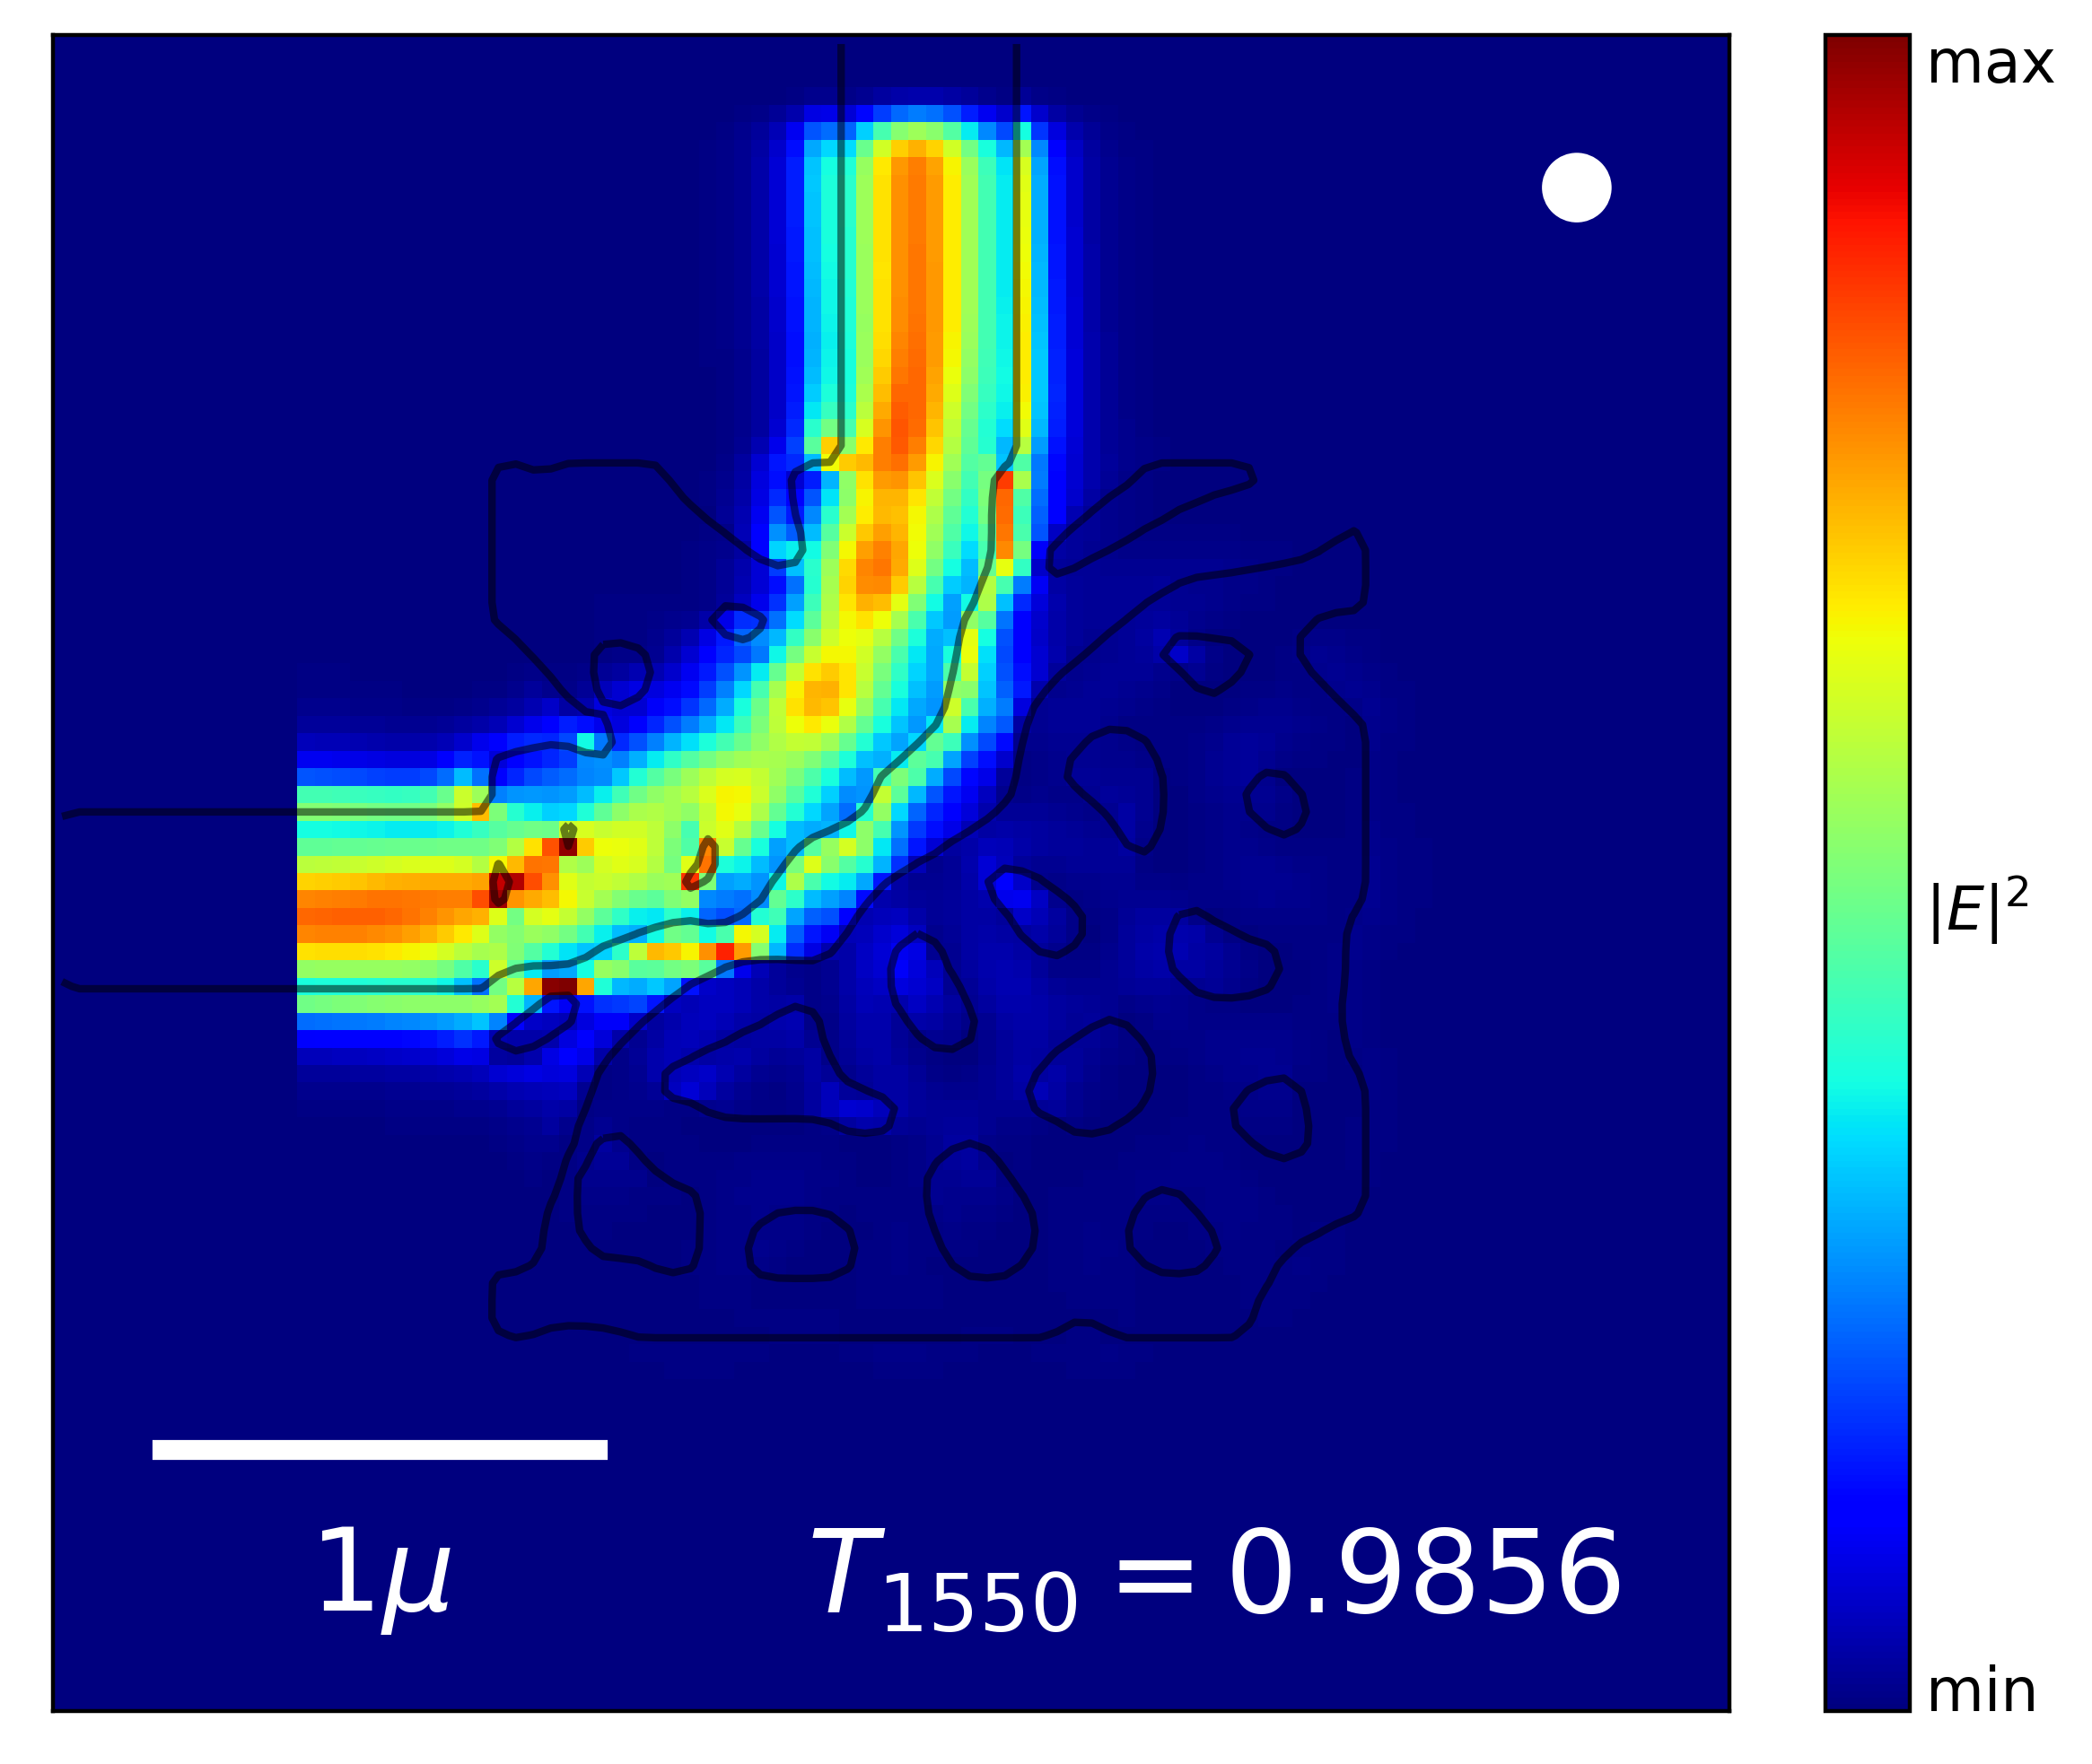
\includegraphics[width=0.33\textwidth]{image/results/bend/L-BFGS-B/visualize_field_disc_512.png} &
      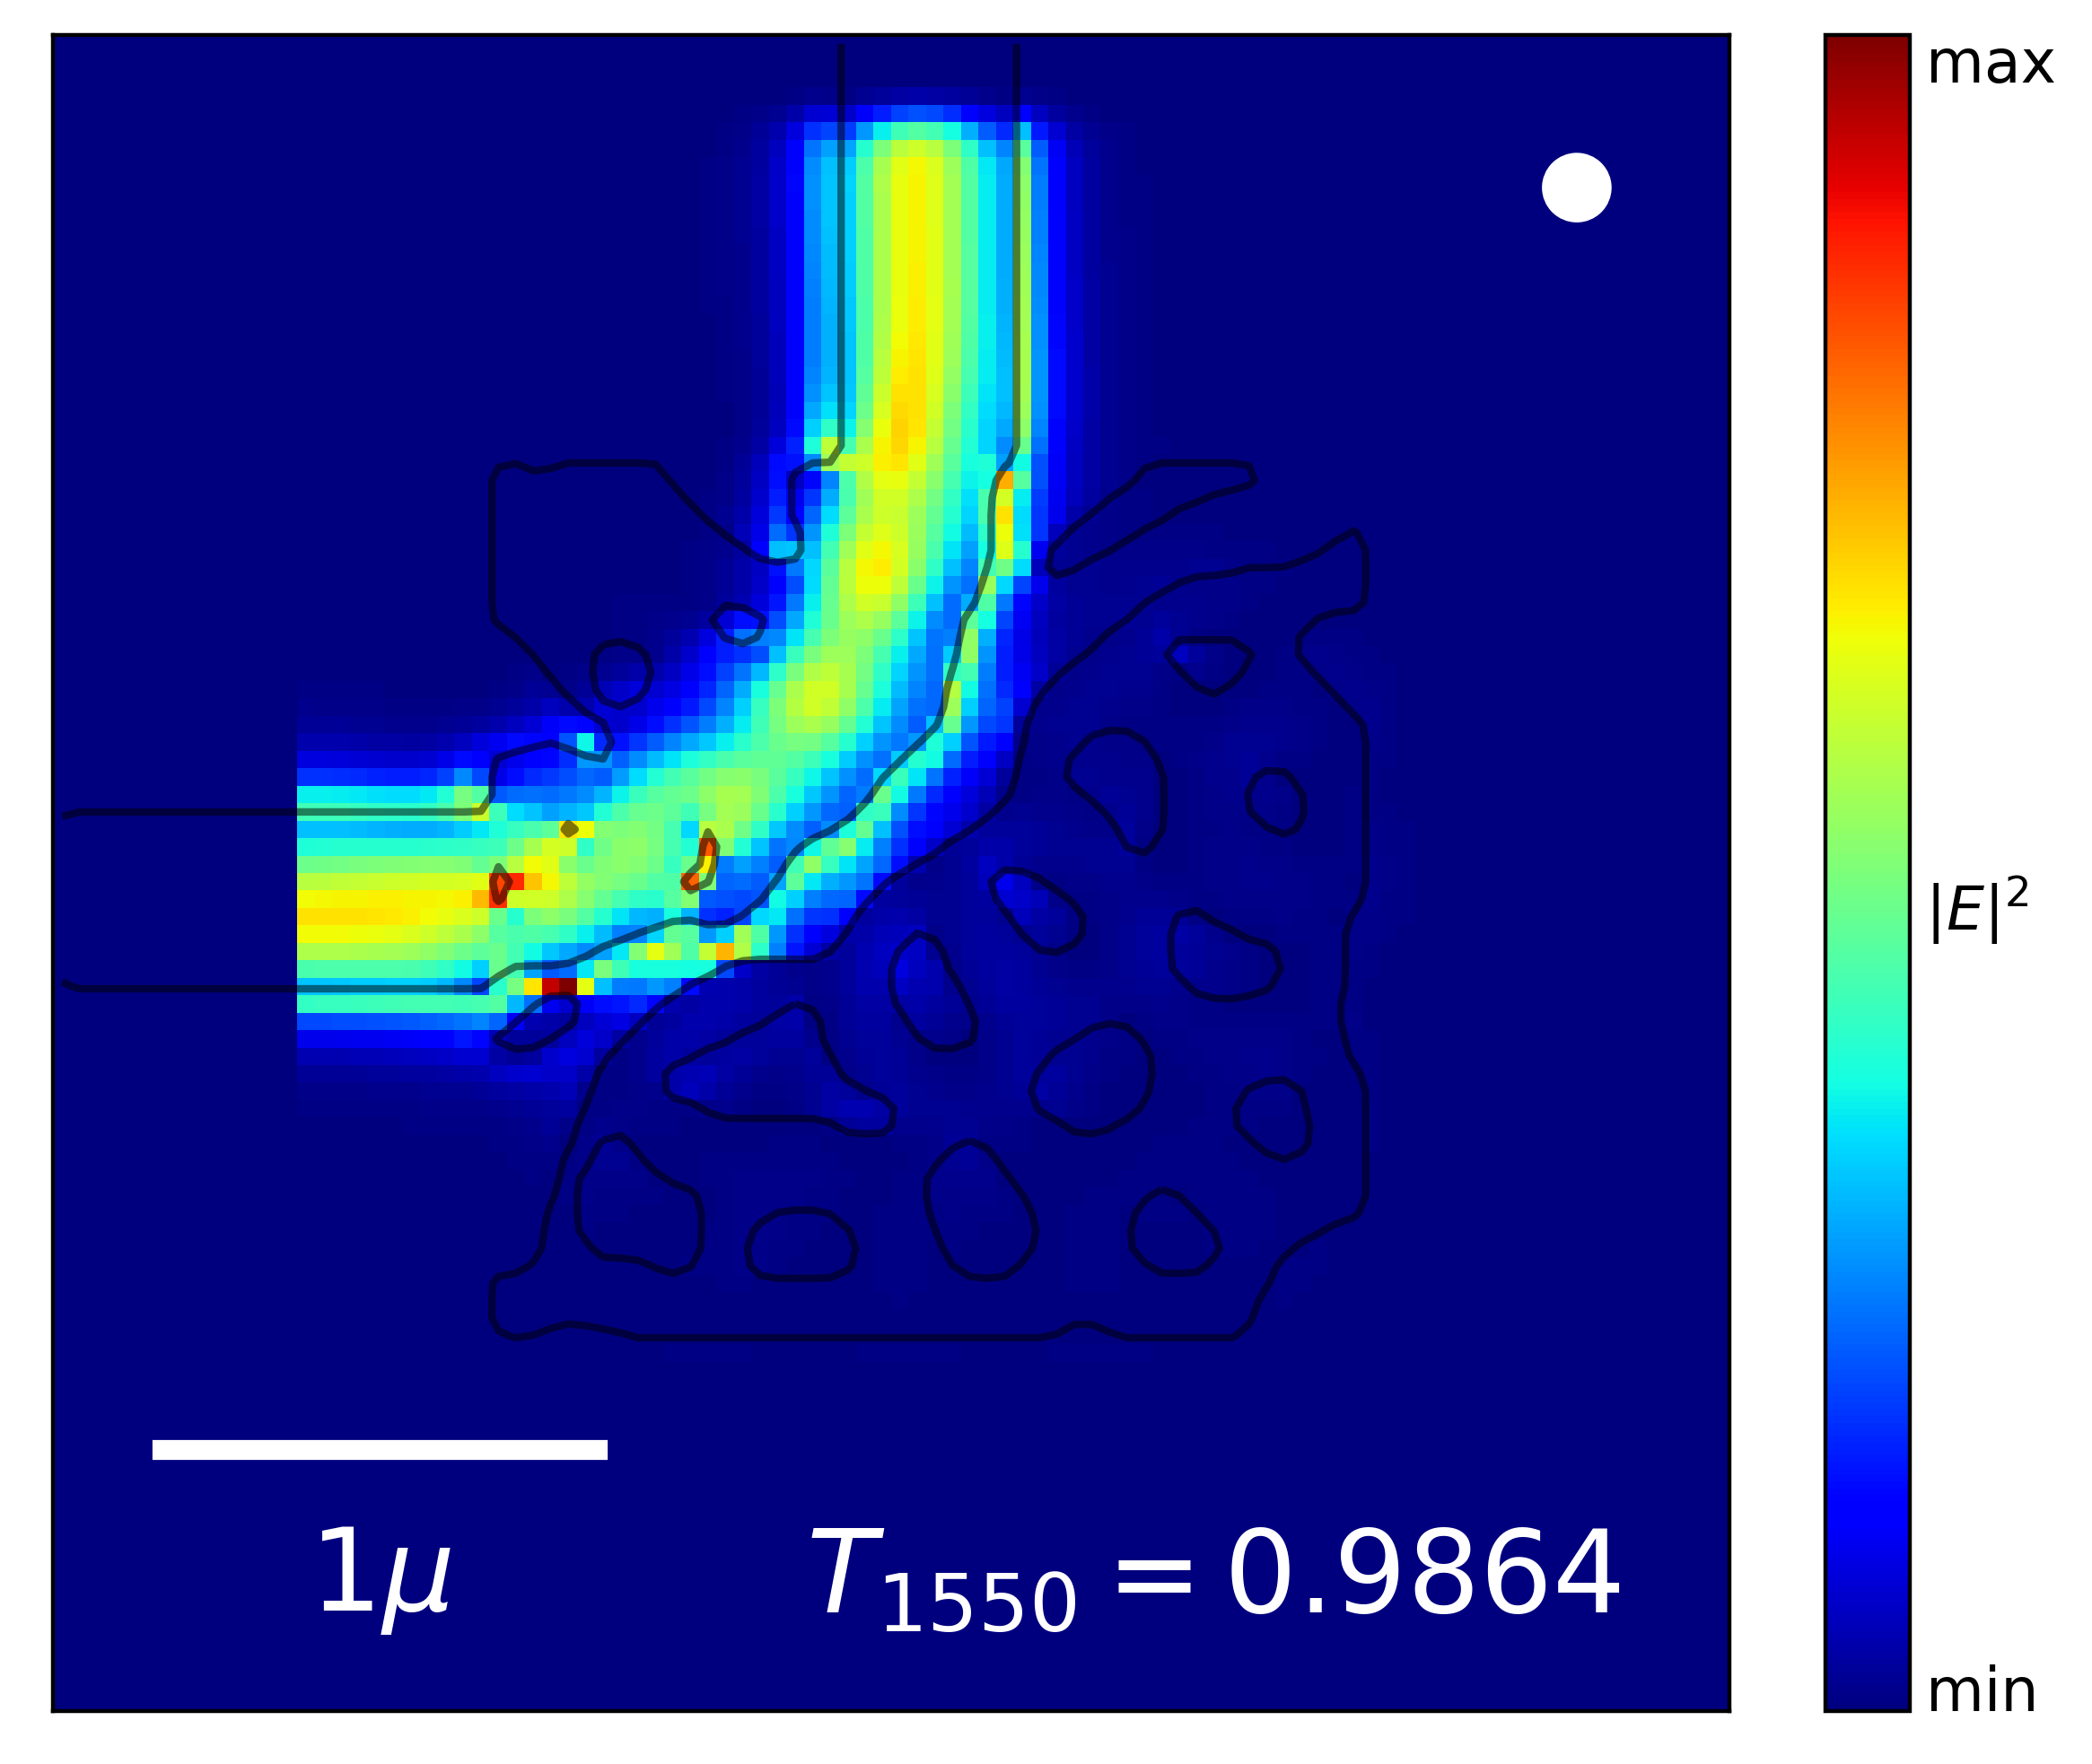
\includegraphics[width=0.33\textwidth]{image/results/bend/L-BFGS-B/visualize_field_fab_512.png} \\
    \hline
    \end{tabular}
    \hspace*{-3cm}
    \caption{Resultados de optimizar el \emph{bend} usando L-BFGS-B}
    \label{tab:opt-LBFGSB-bend}
\end{table}

% Bend - CMA-ES
\begin{table}[ht]
    \centering
    \vspace*{-2.5cm}
    \hspace*{-3cm}
    \begin{tabular}{|c|c|c|c|}
    \hline 
    \emph{Seed} & Opt. continua & Opt. discreta &  Opt. de fabricación \\
    \hline
      \multirow{2}{*}{128} &
      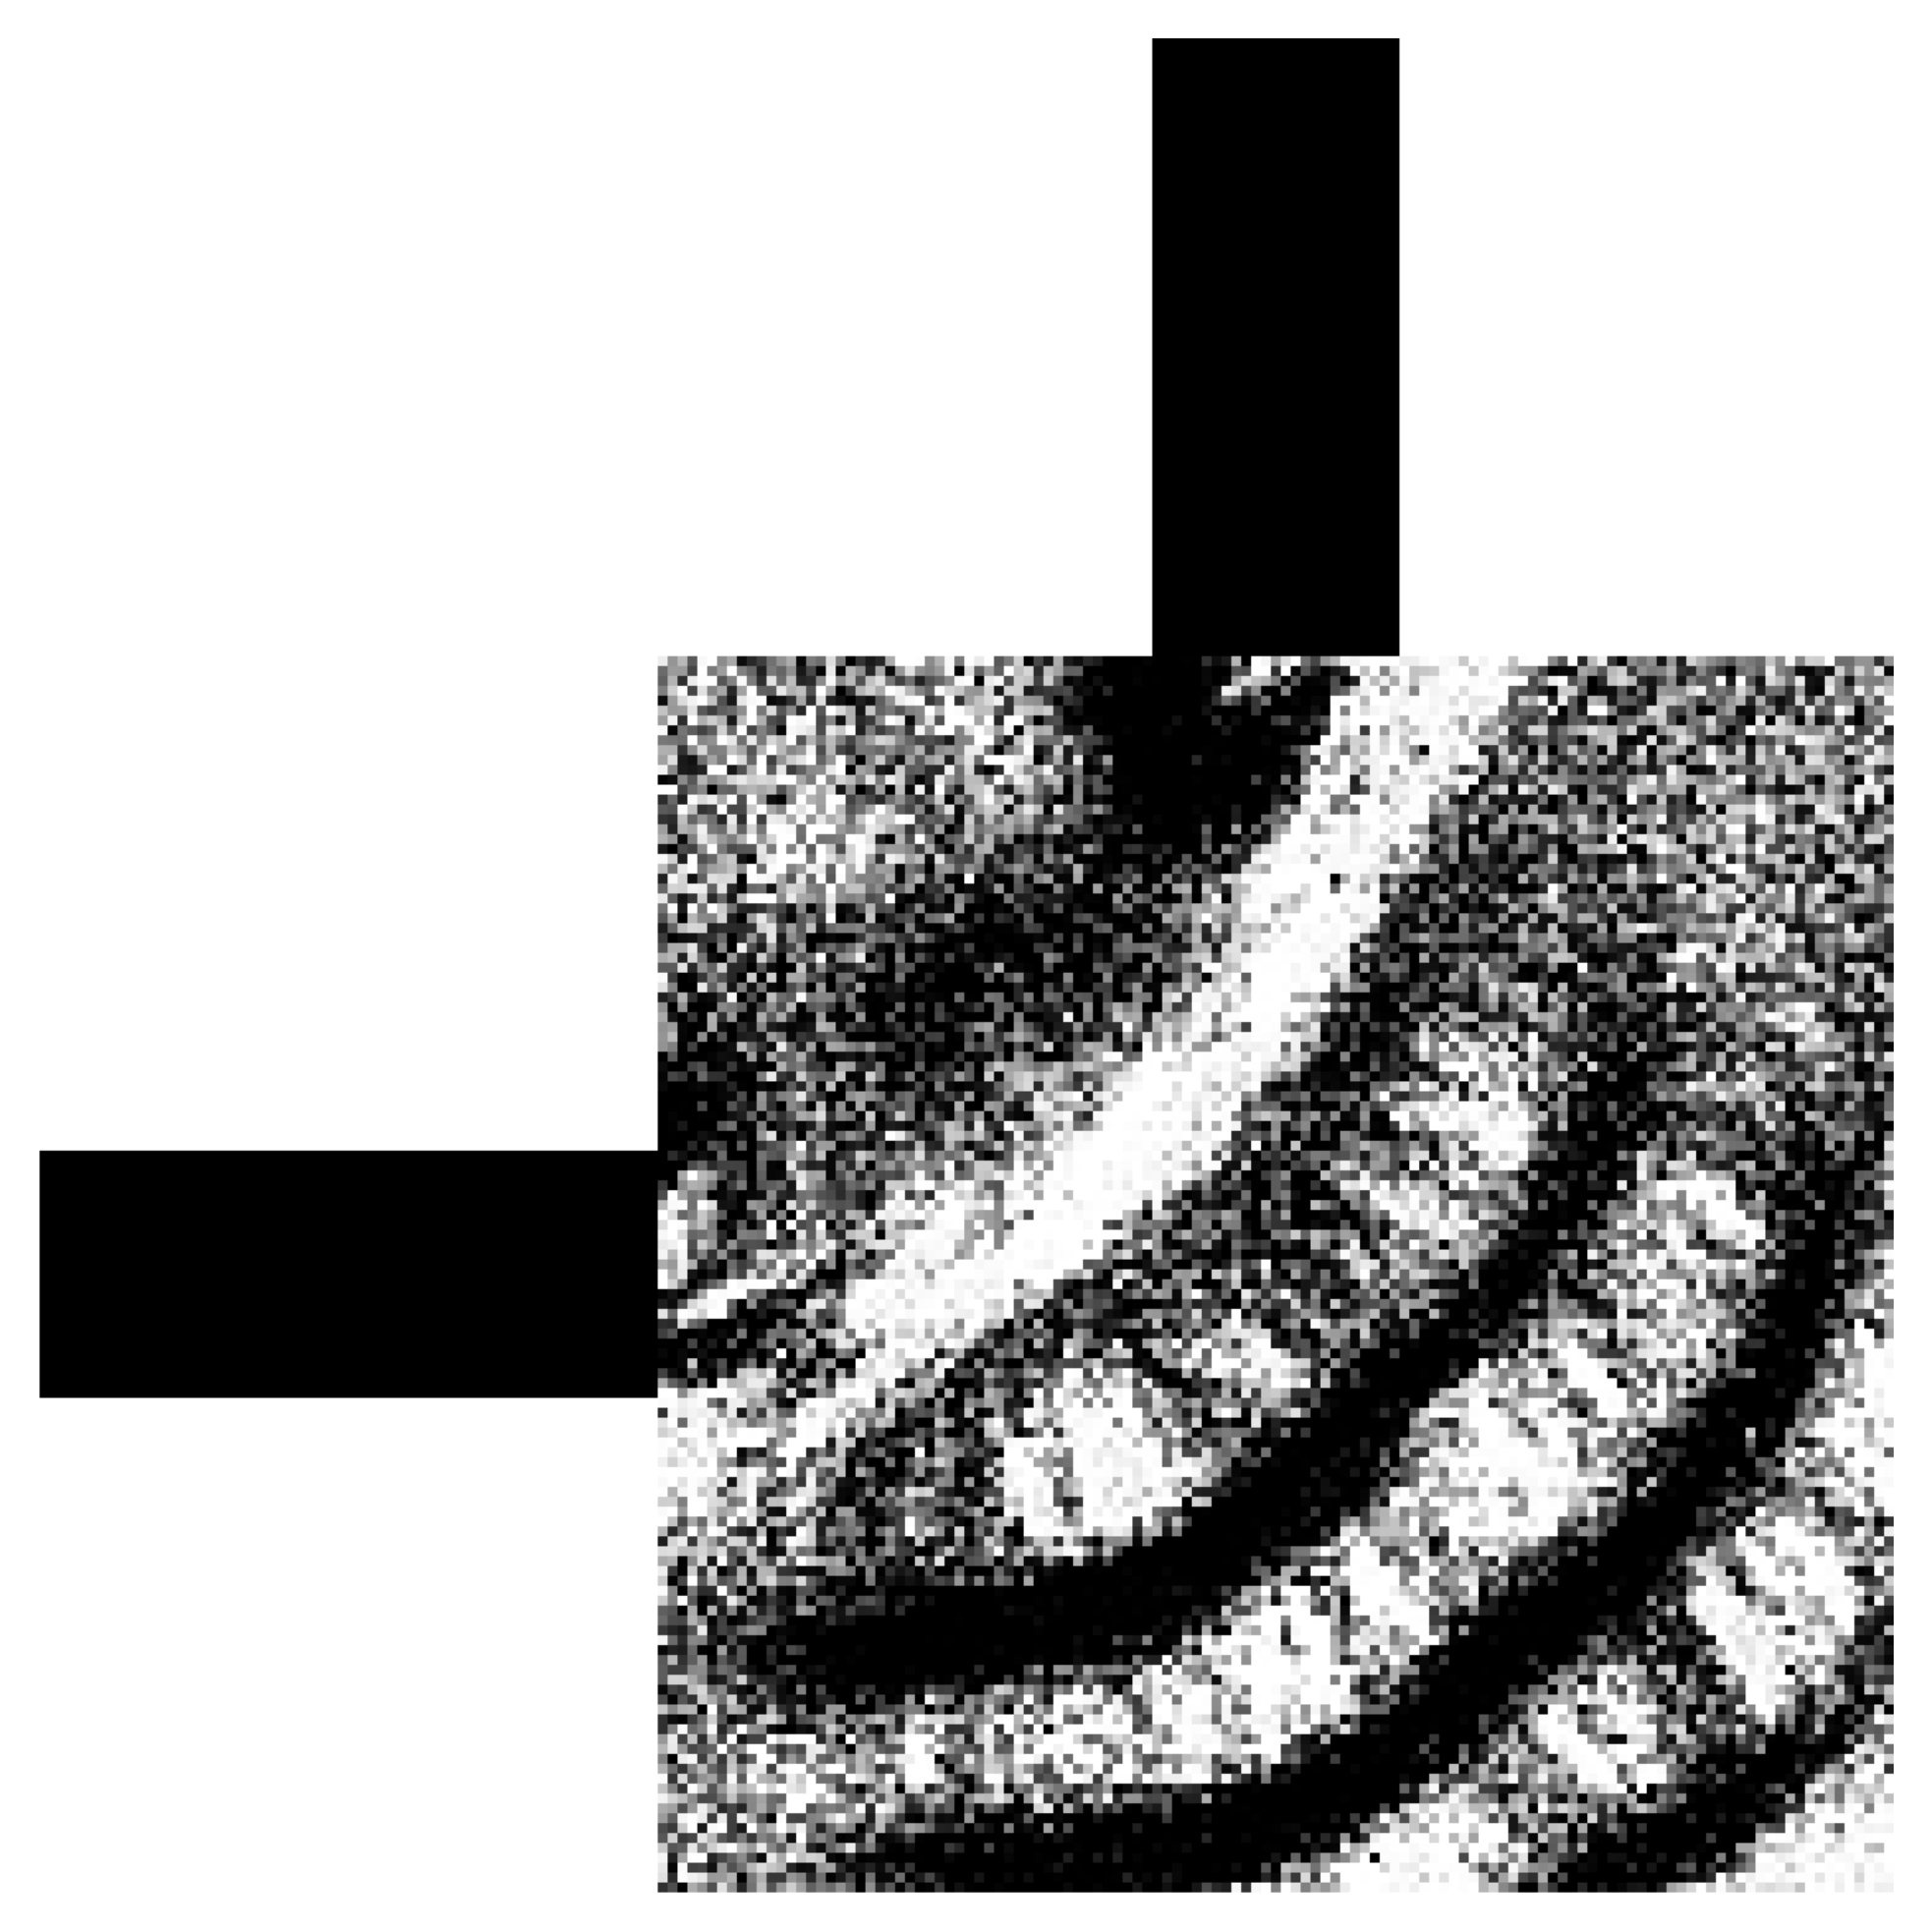
\includegraphics[width=0.20\textwidth]{image/results/bend/CMA-ES/visualize_eps_cont_128.png} &
      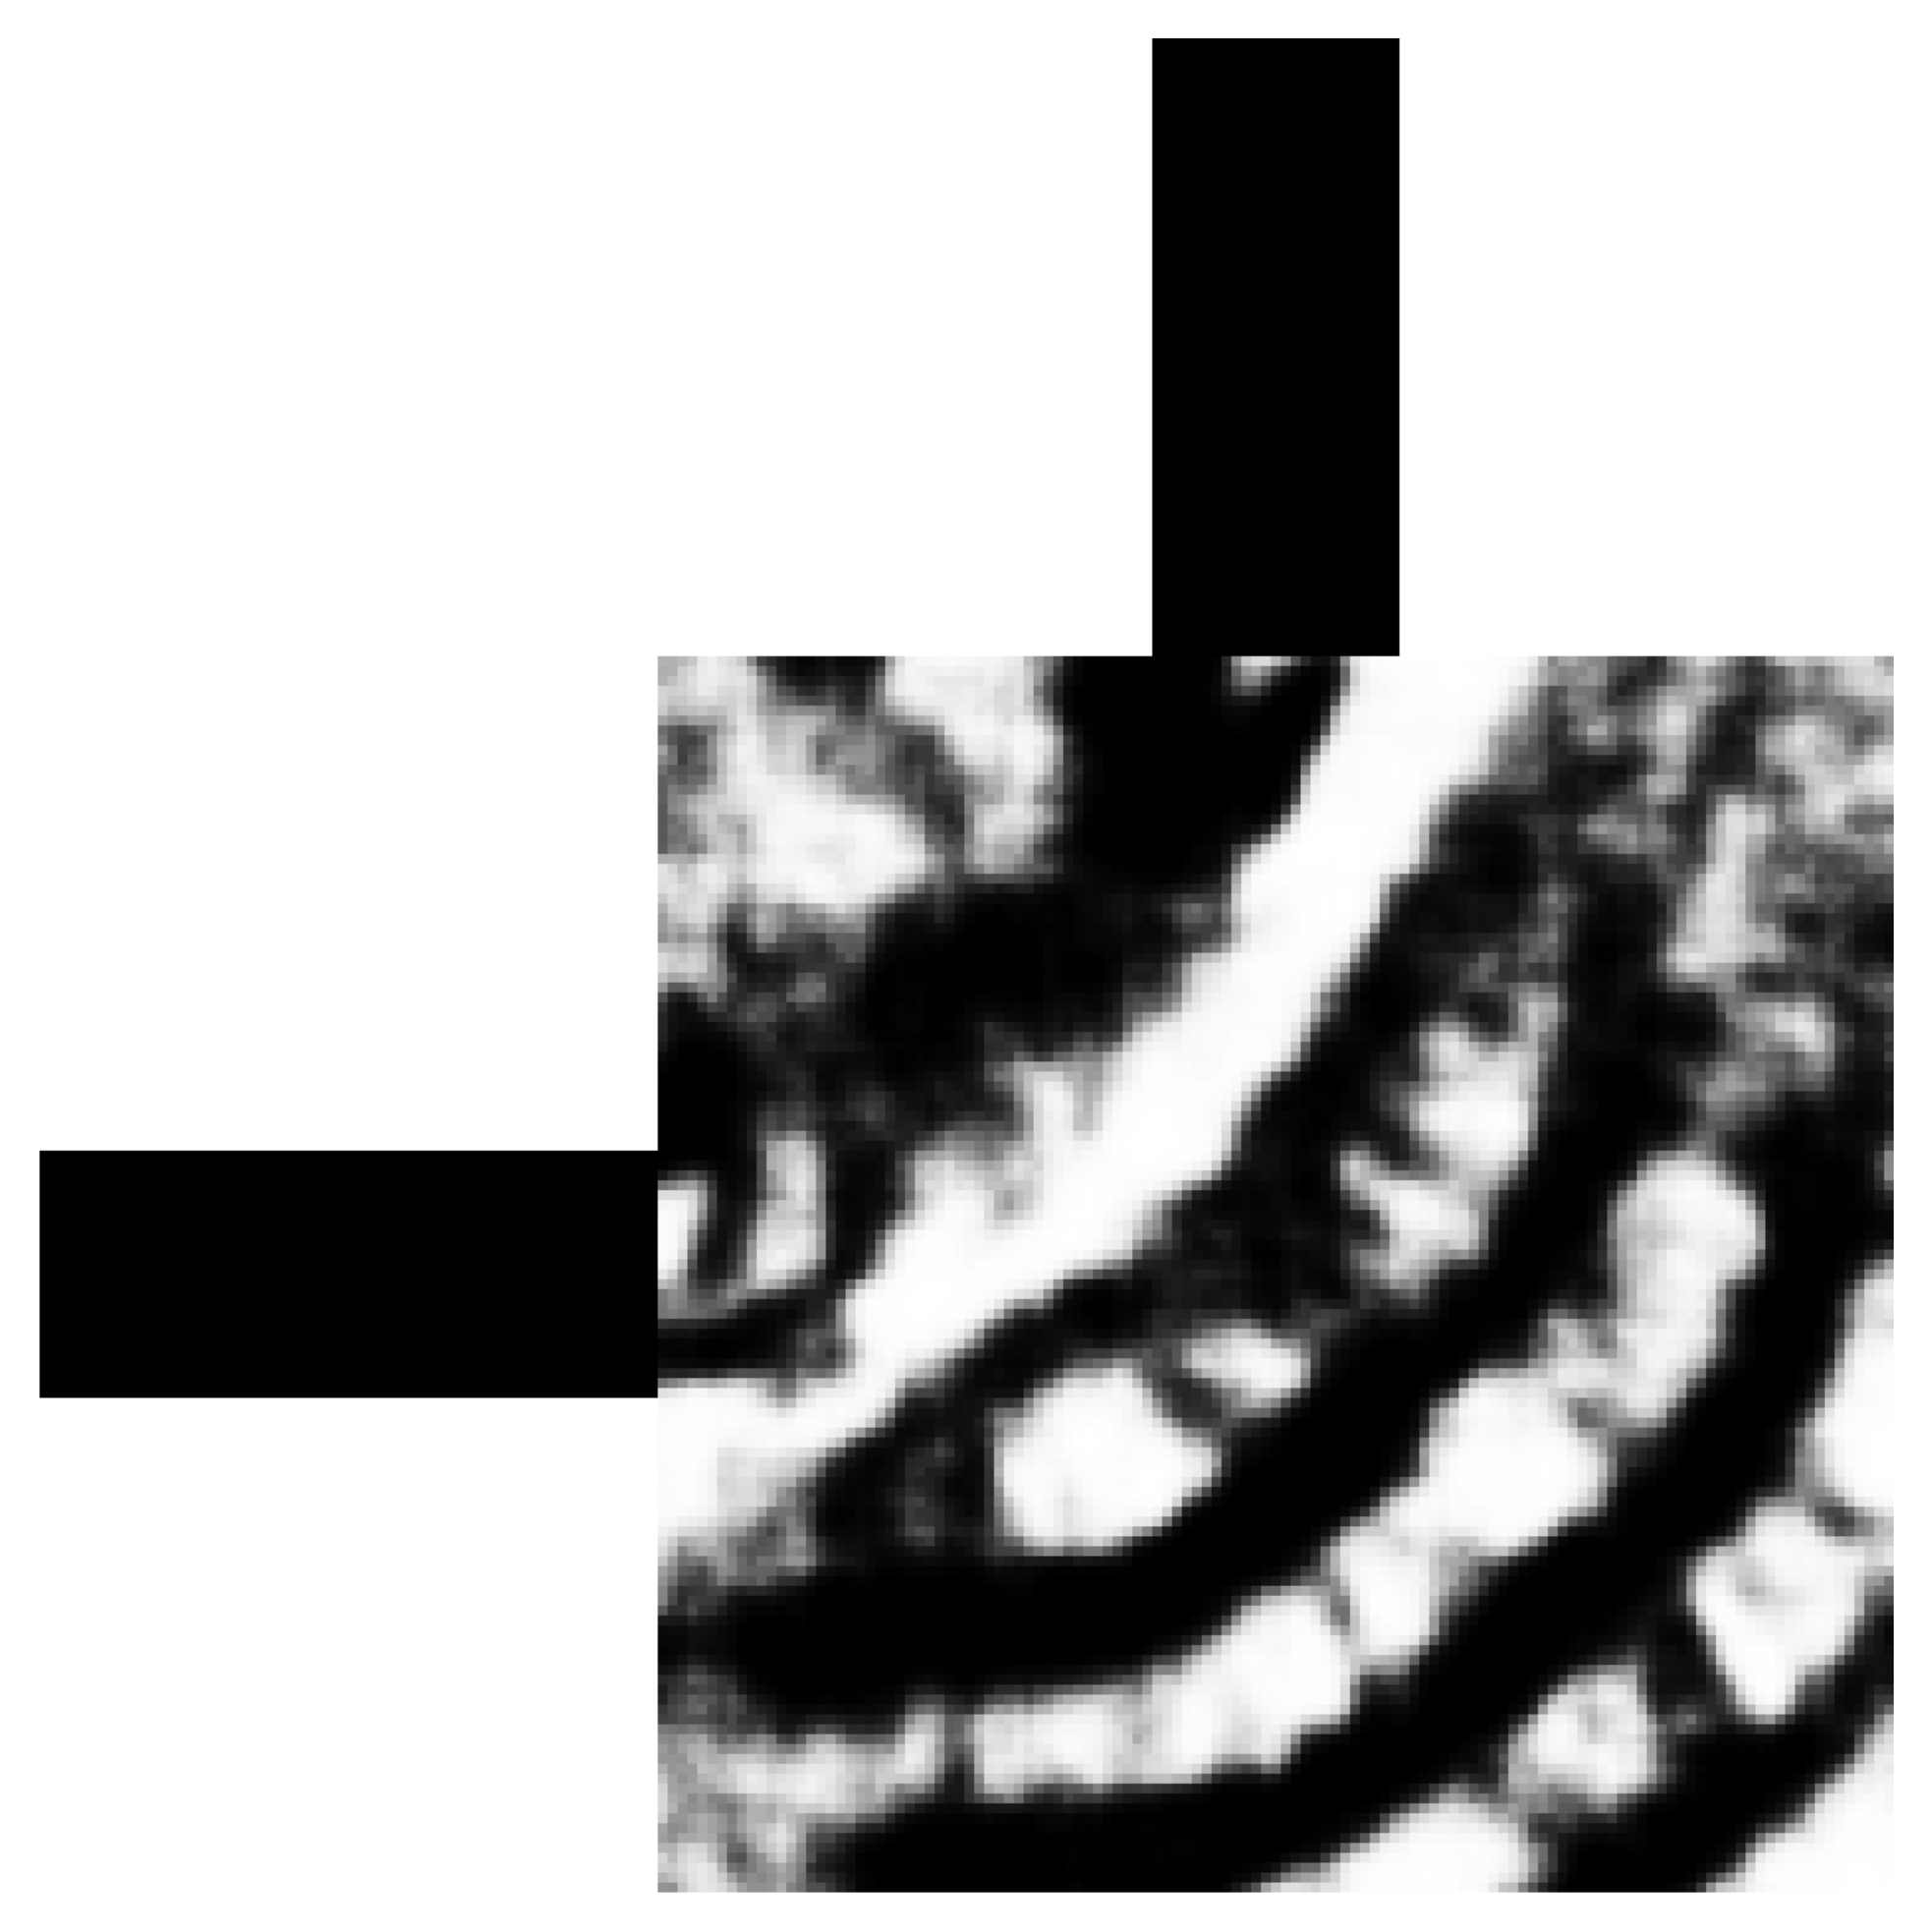
\includegraphics[width=0.20\textwidth]{image/results/bend/CMA-ES/visualize_eps_disc_128.png} &
      
\includegraphics[width=0.20\textwidth]{image/results/bend/CMA-ES/visualize_eps_fab_128.png} \\
      \cline{2-4}
      &
      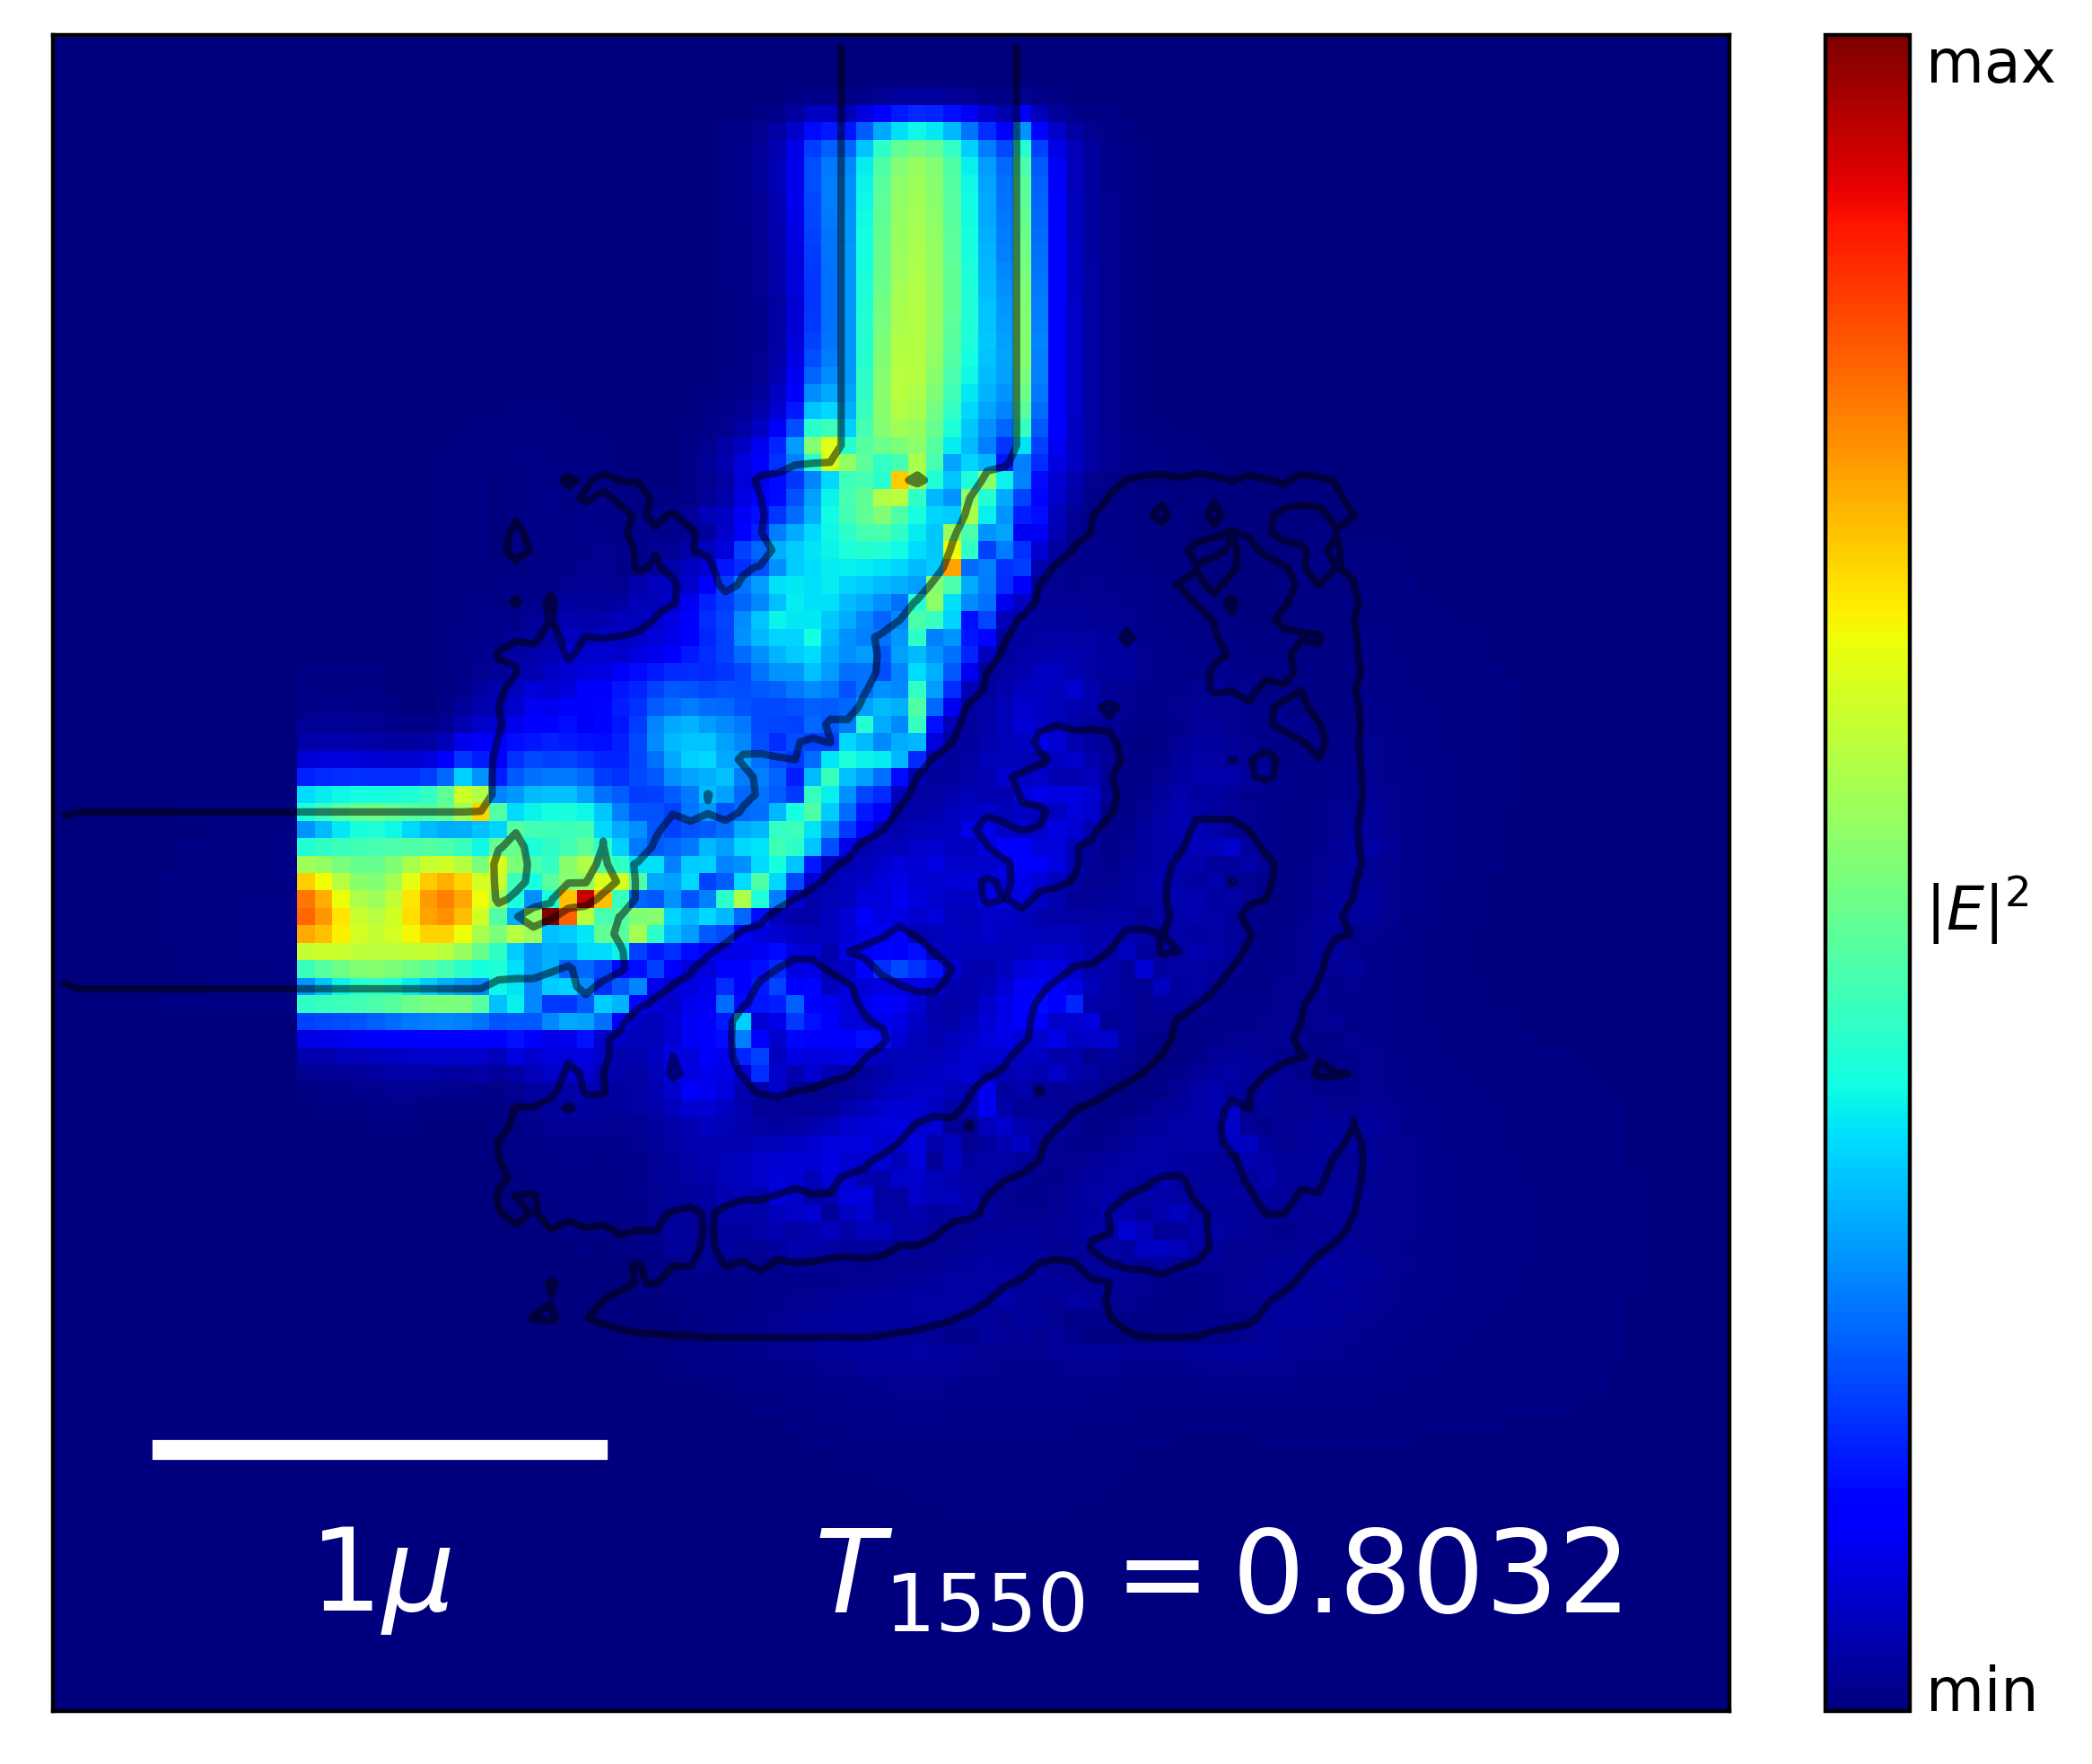
\includegraphics[width=0.33\textwidth]{image/results/bend/CMA-ES/visualize_field_cont_128.png} &
      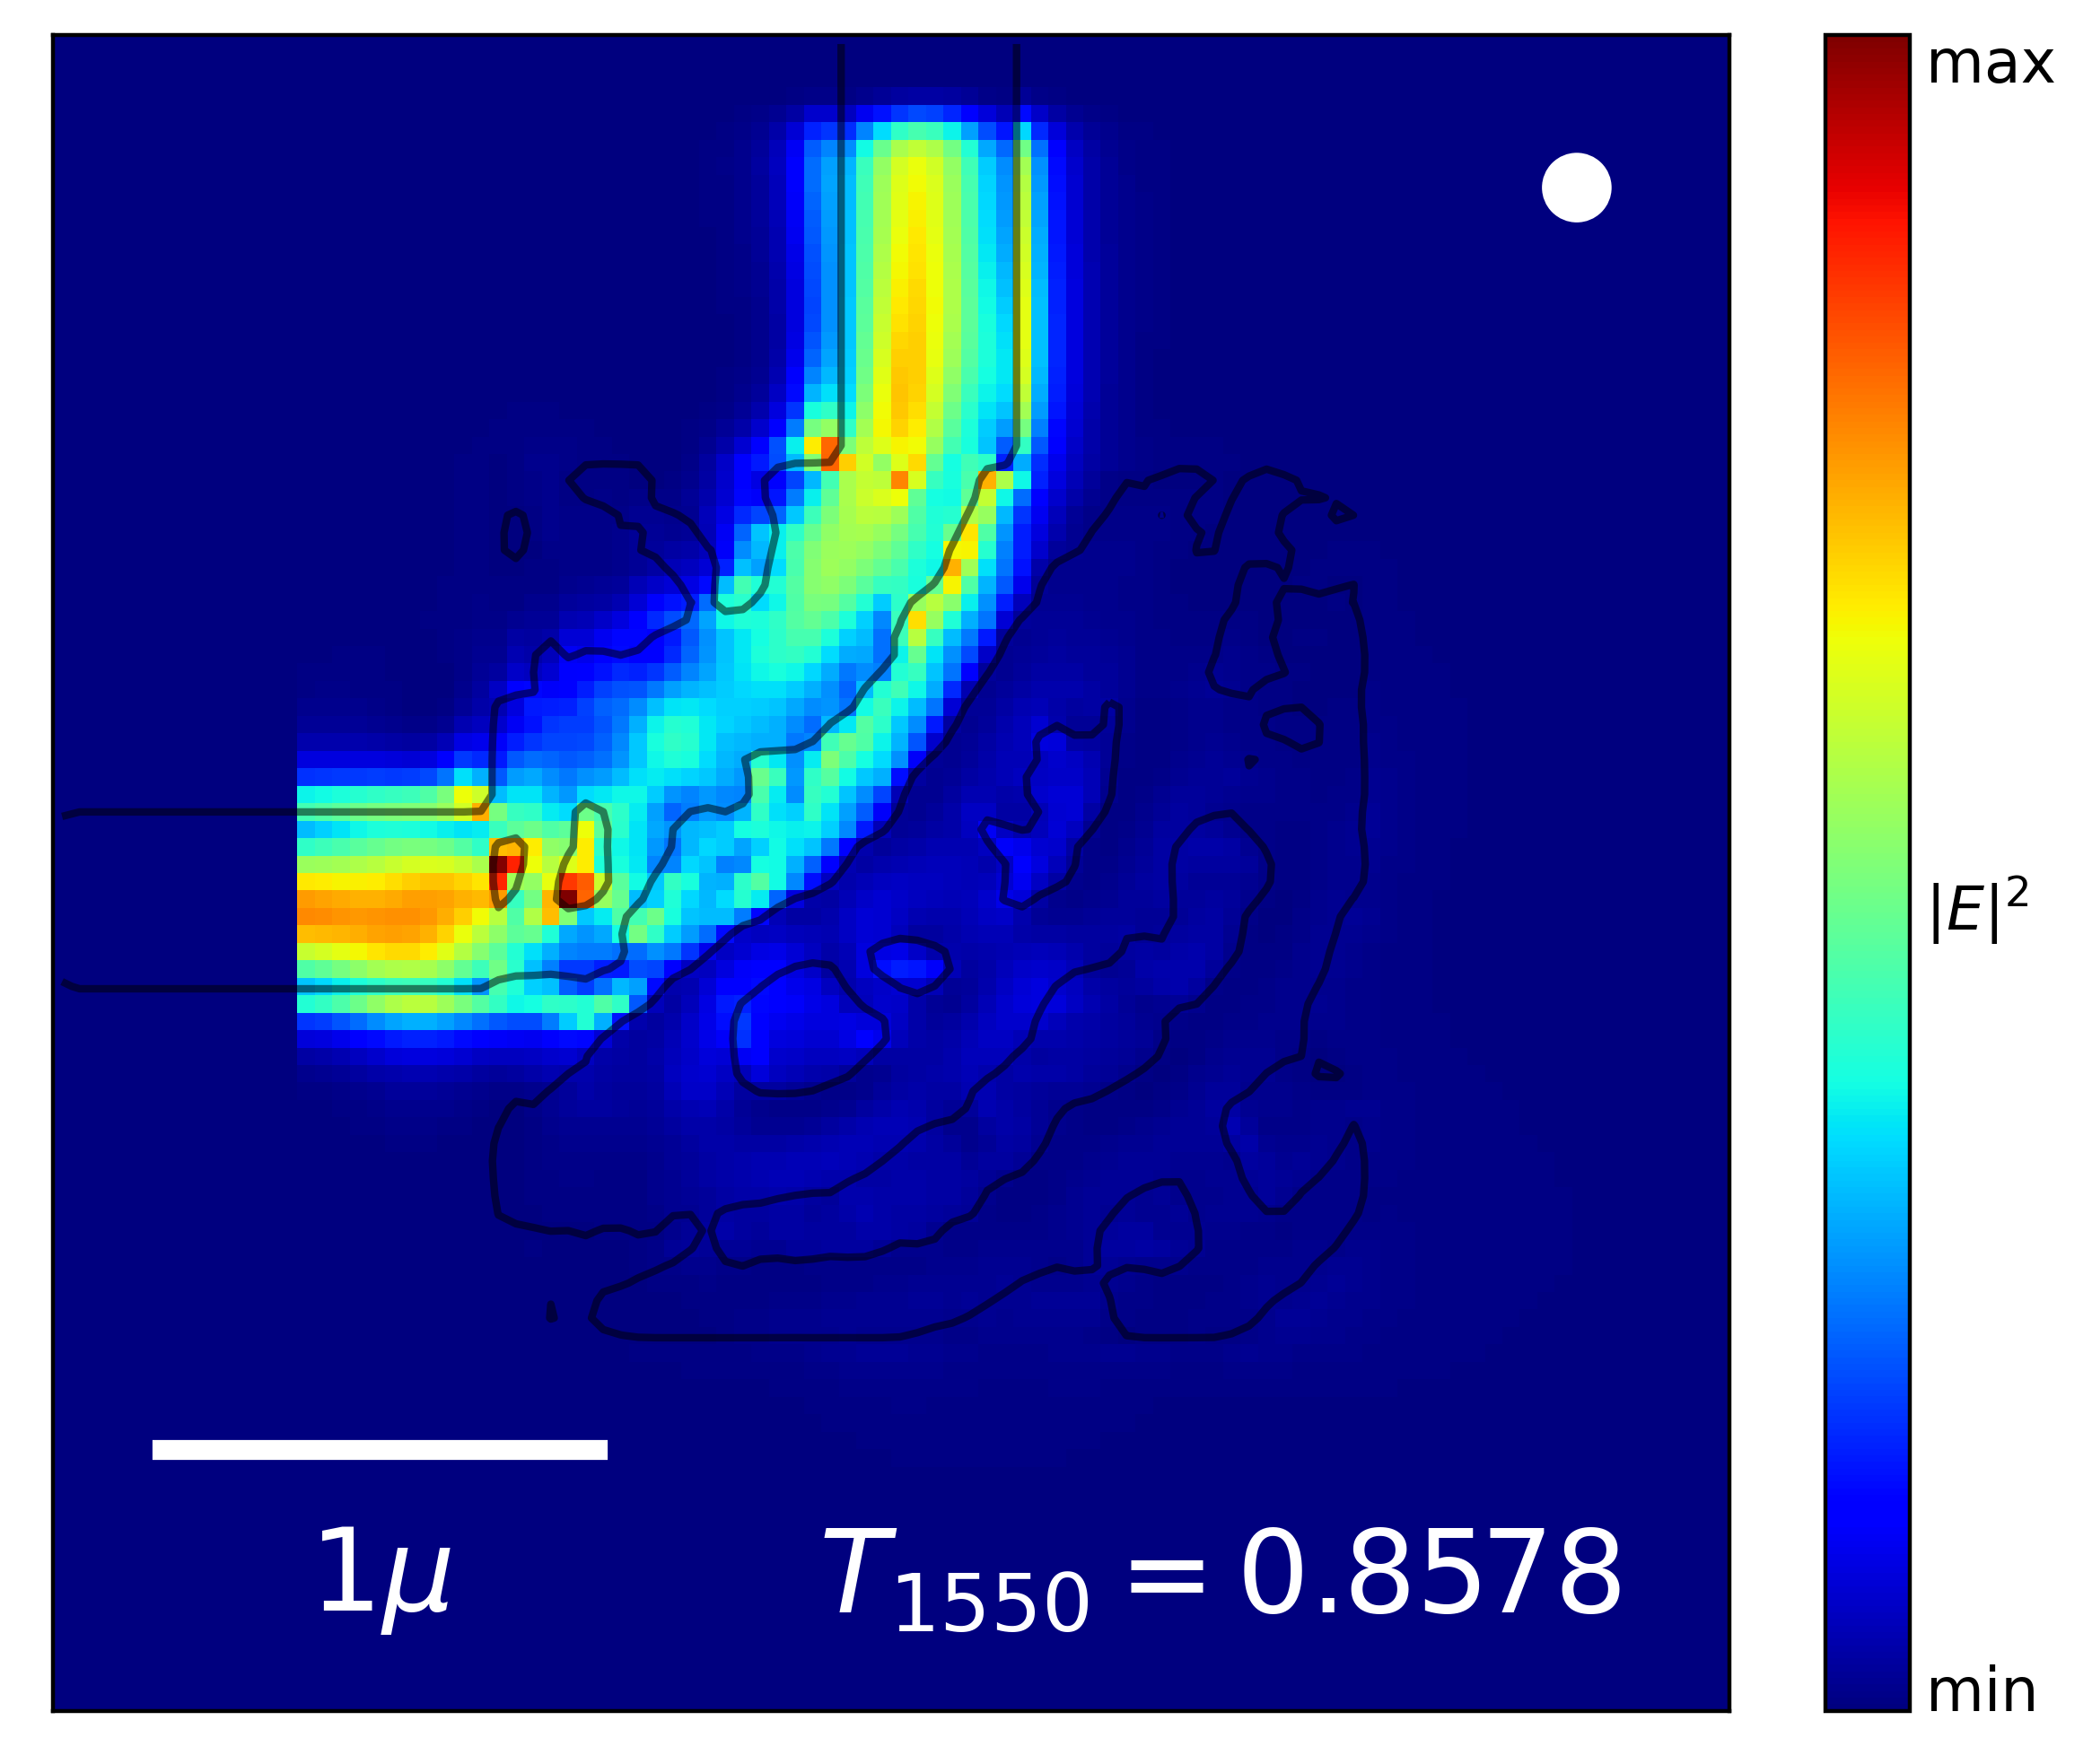
\includegraphics[width=0.33\textwidth]{image/results/bend/CMA-ES/visualize_field_disc_128.png} &
      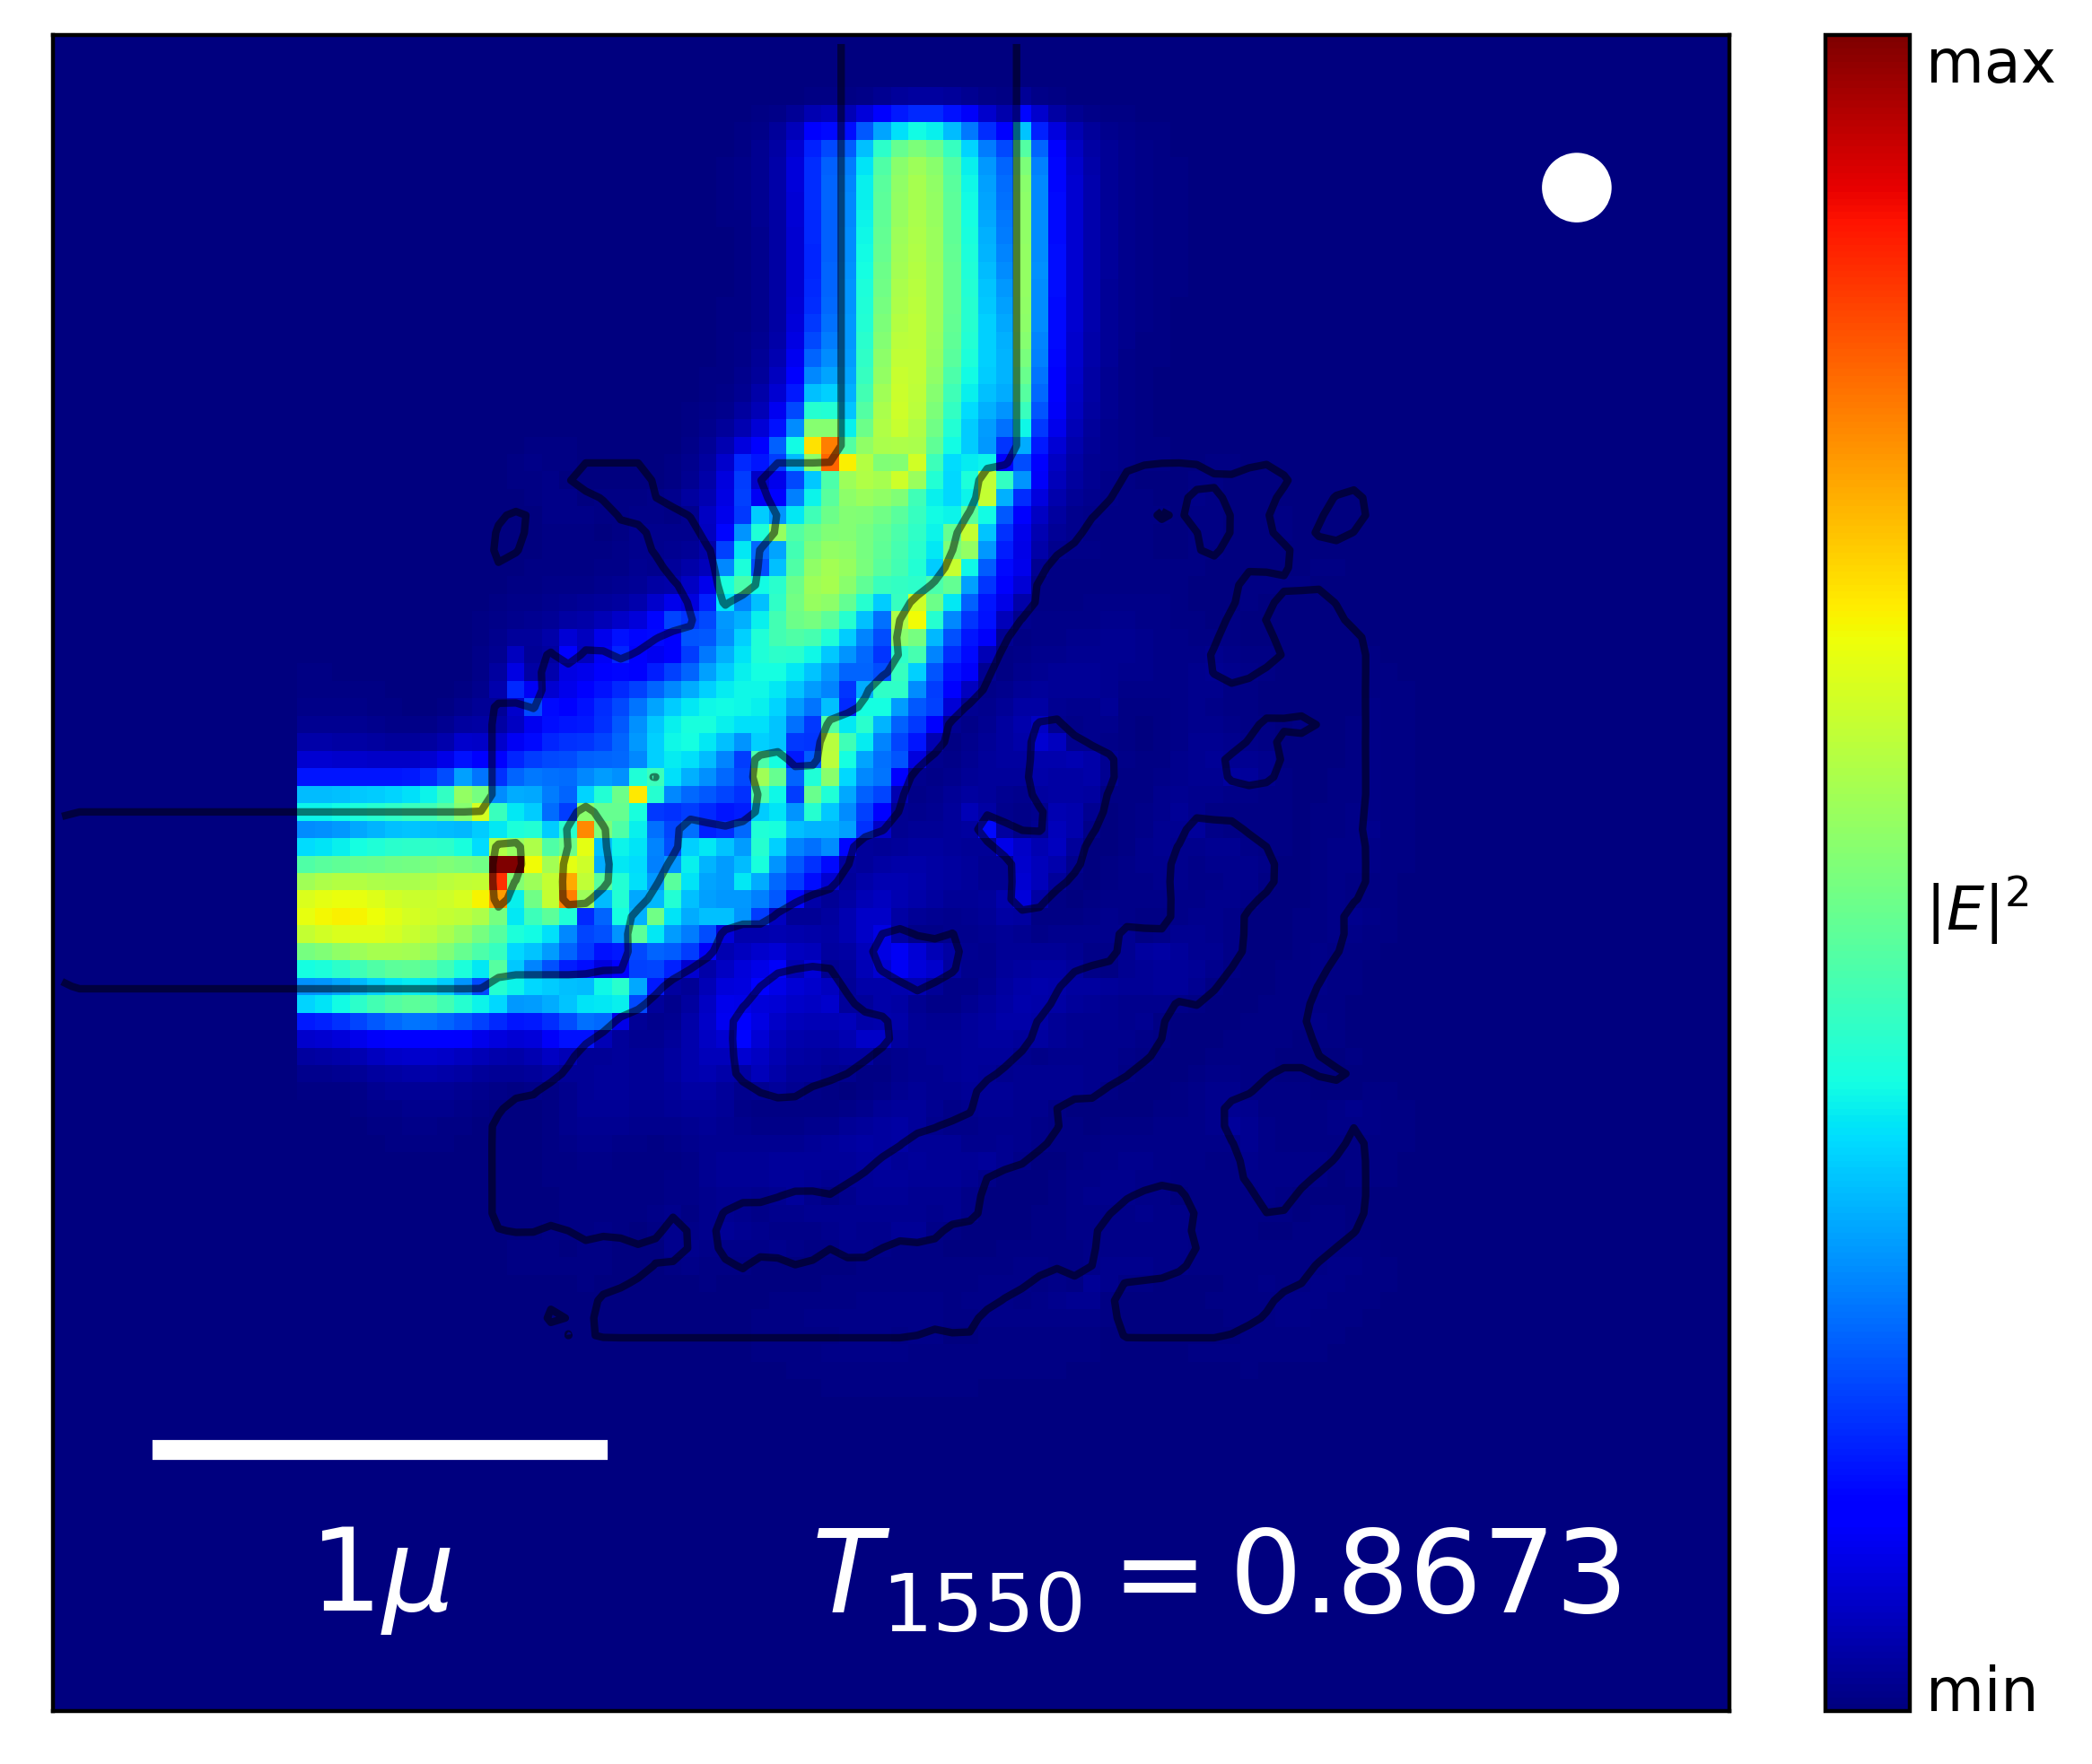
\includegraphics[width=0.33\textwidth]{image/results/bend/CMA-ES/visualize_field_fab_128.png} \\
    \hline
      \multirow{2}{*}{256} &
      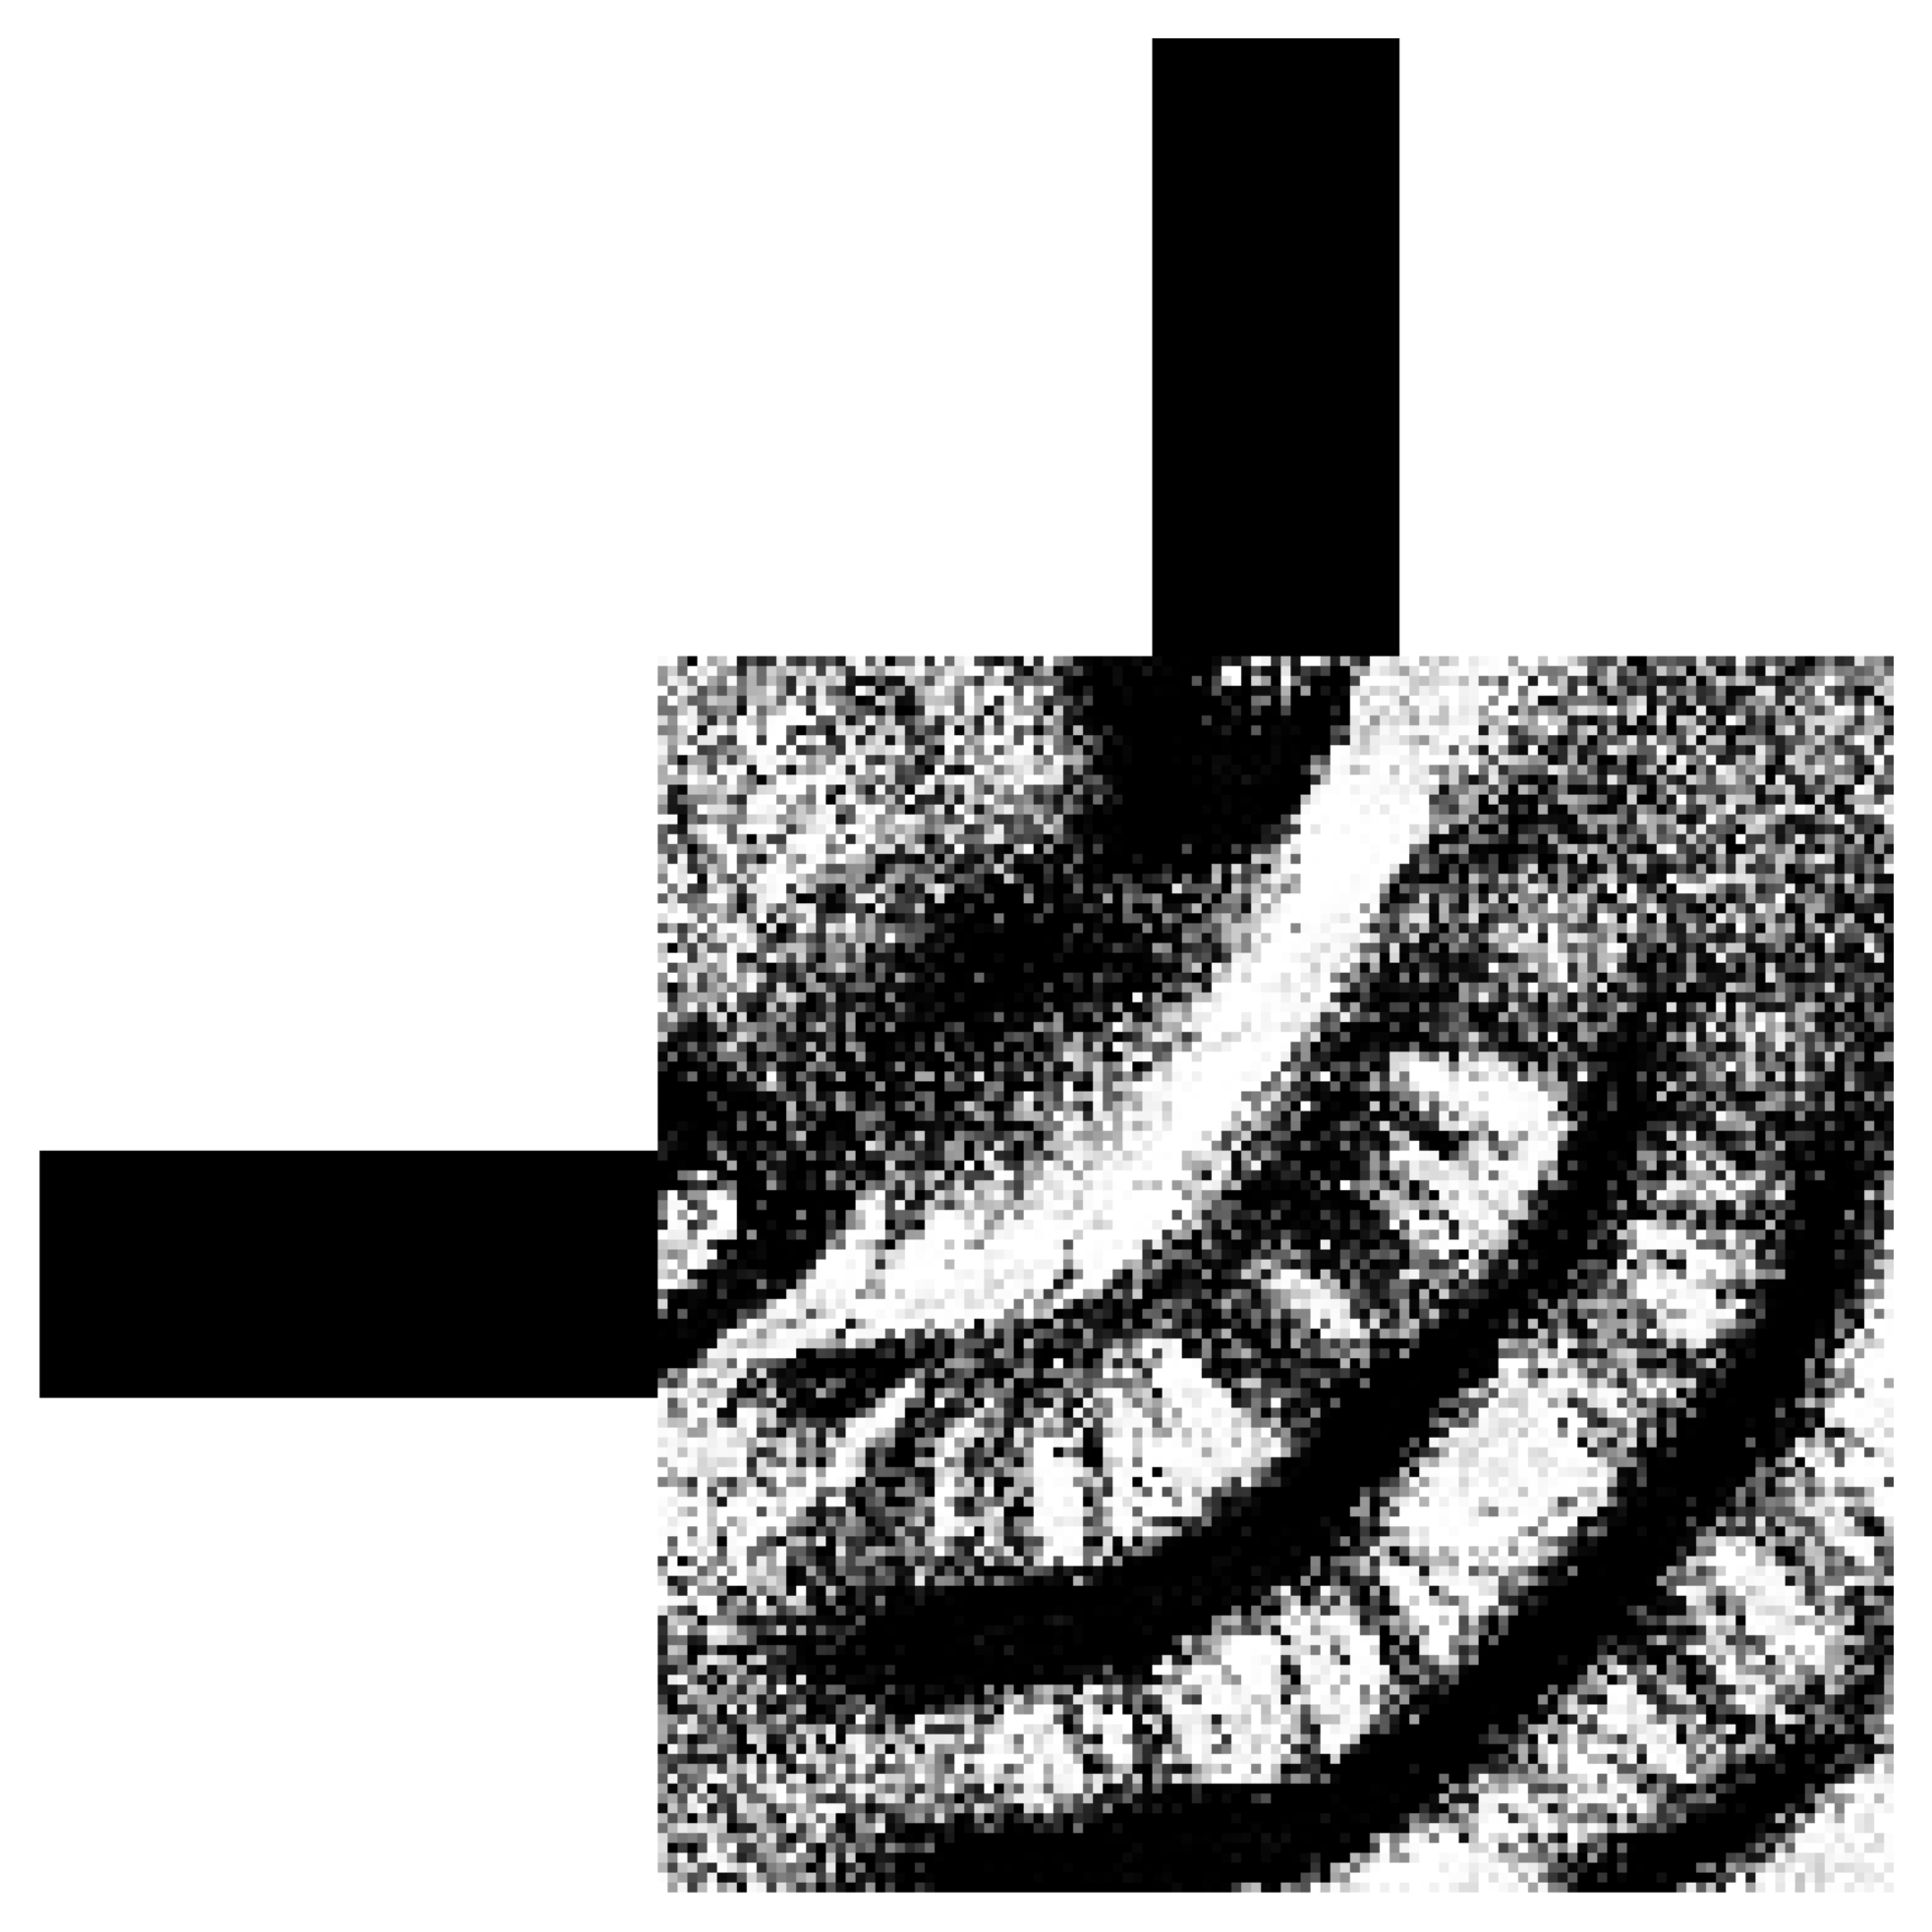
\includegraphics[width=0.20\textwidth]{image/results/bend/CMA-ES/visualize_eps_cont_256.png} &
      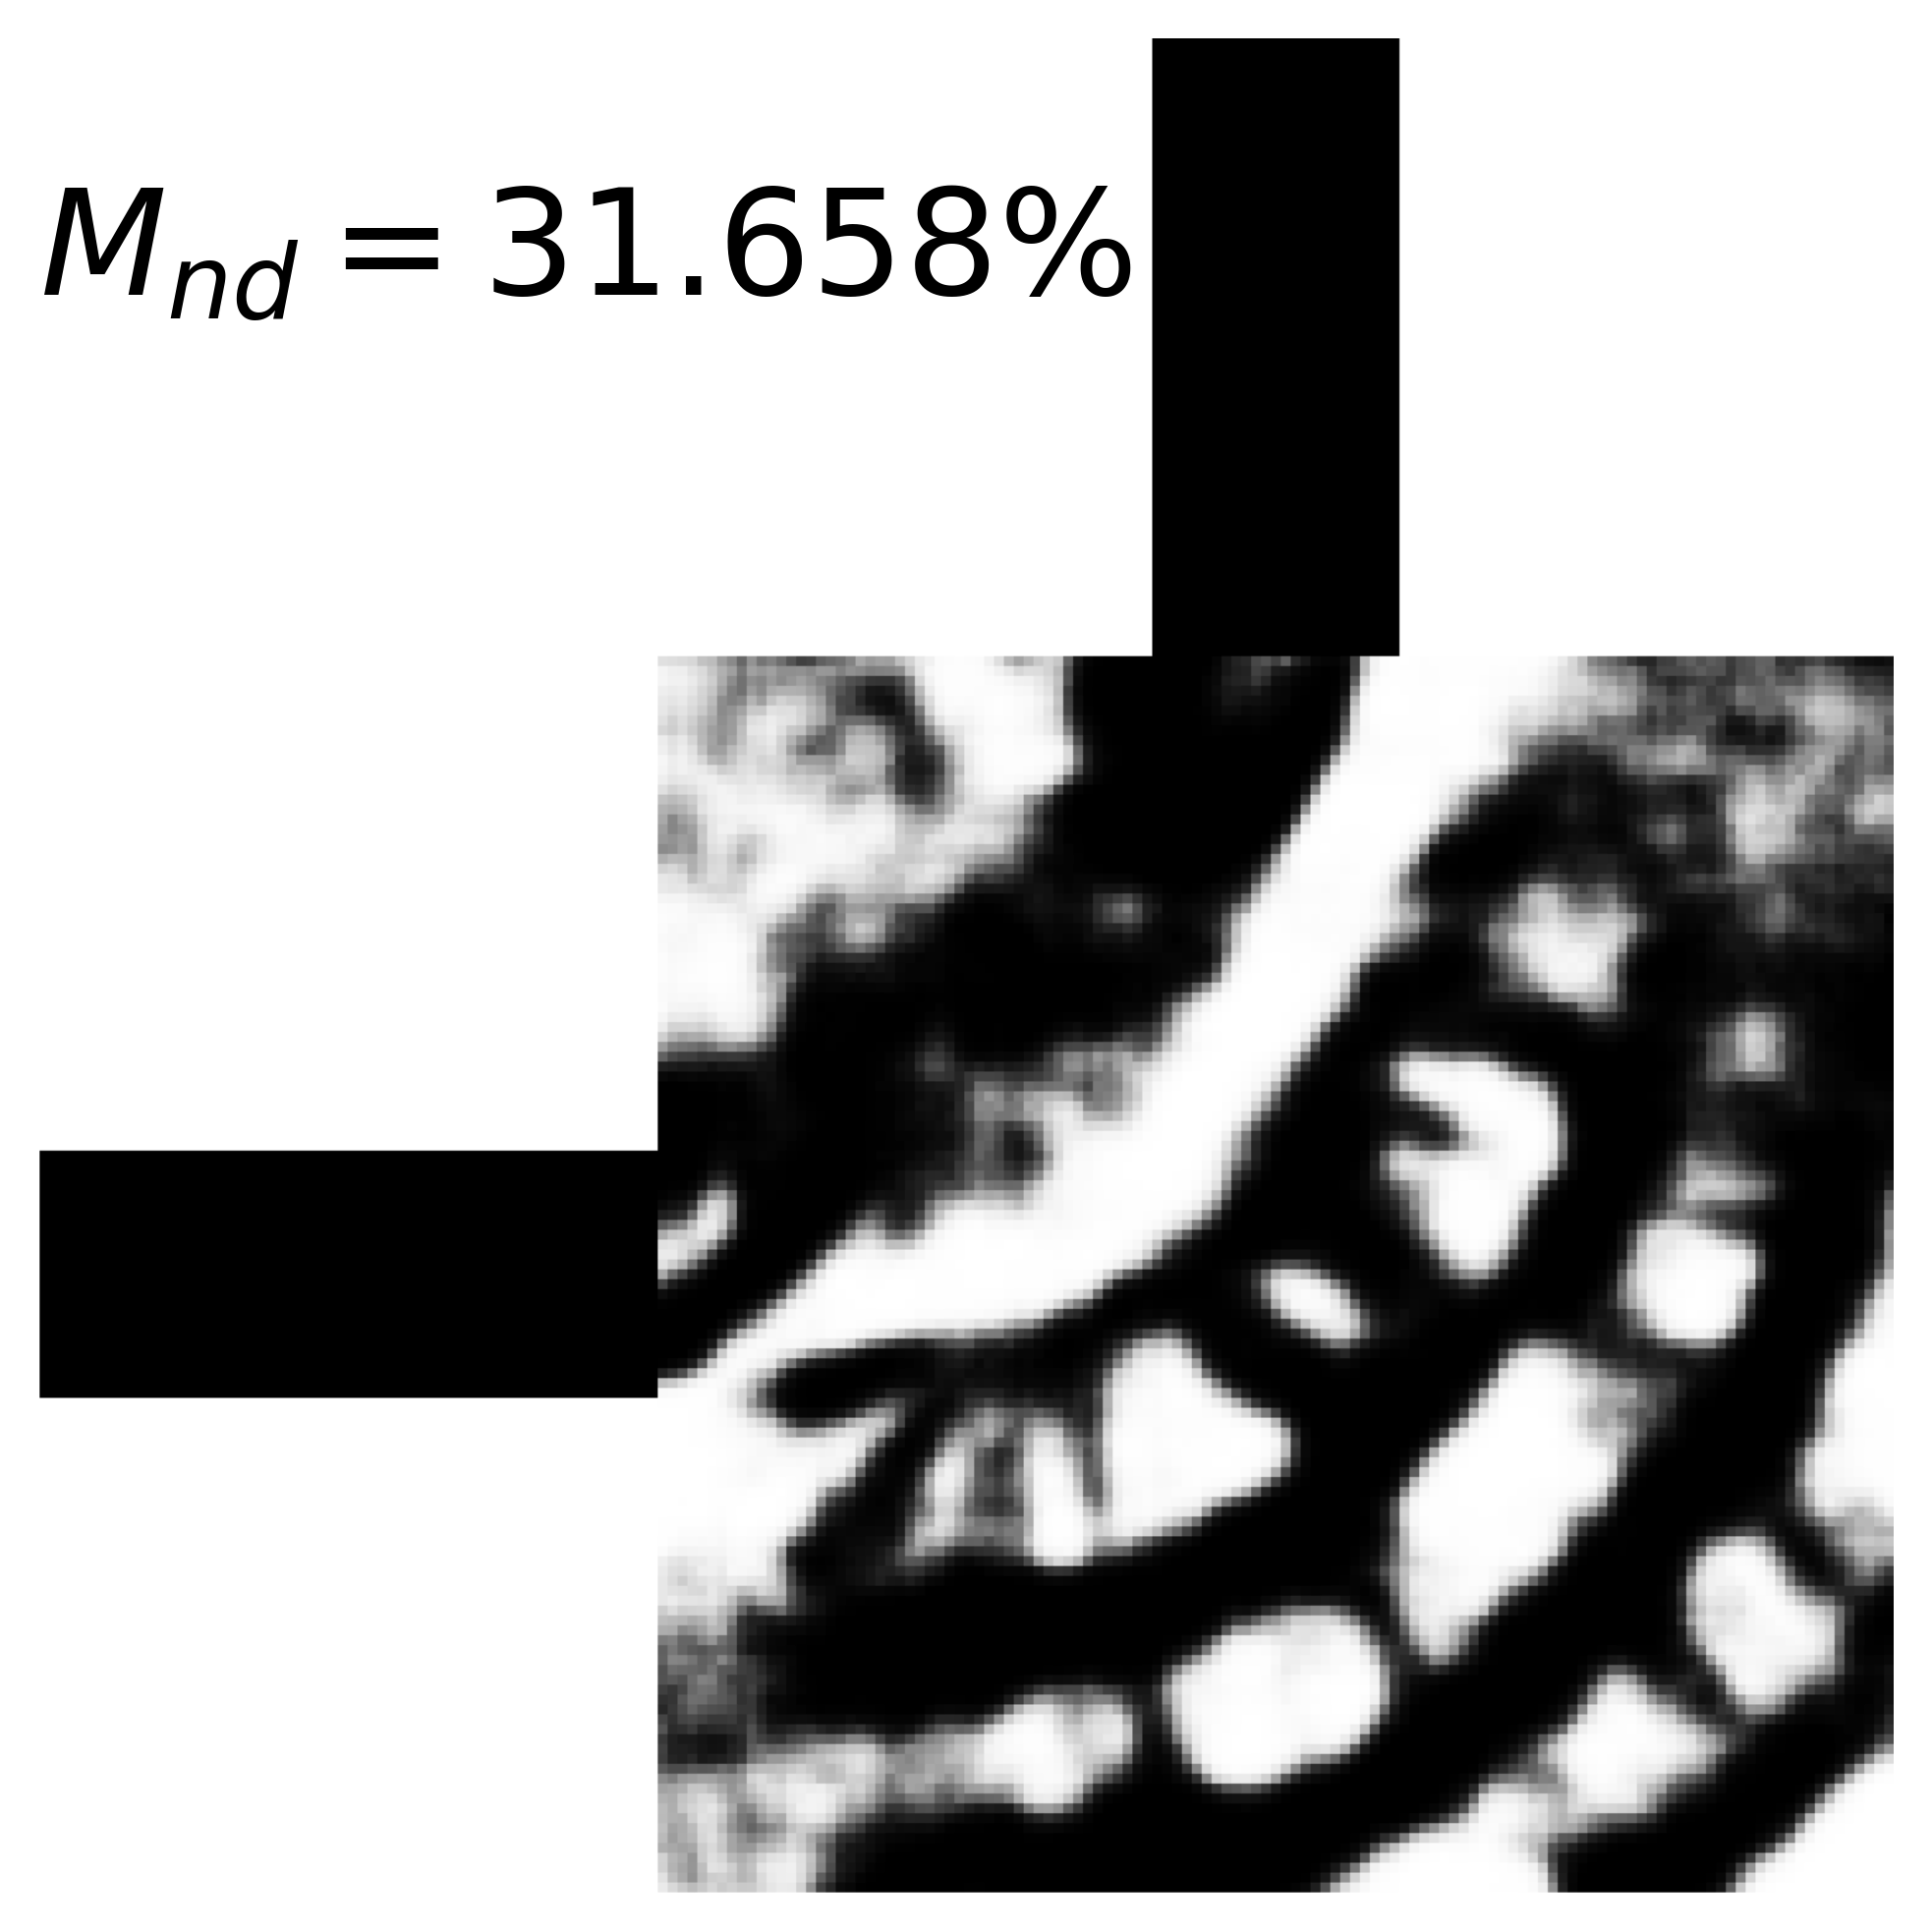
\includegraphics[width=0.20\textwidth]{image/results/bend/CMA-ES/visualize_eps_disc_256.png} &
      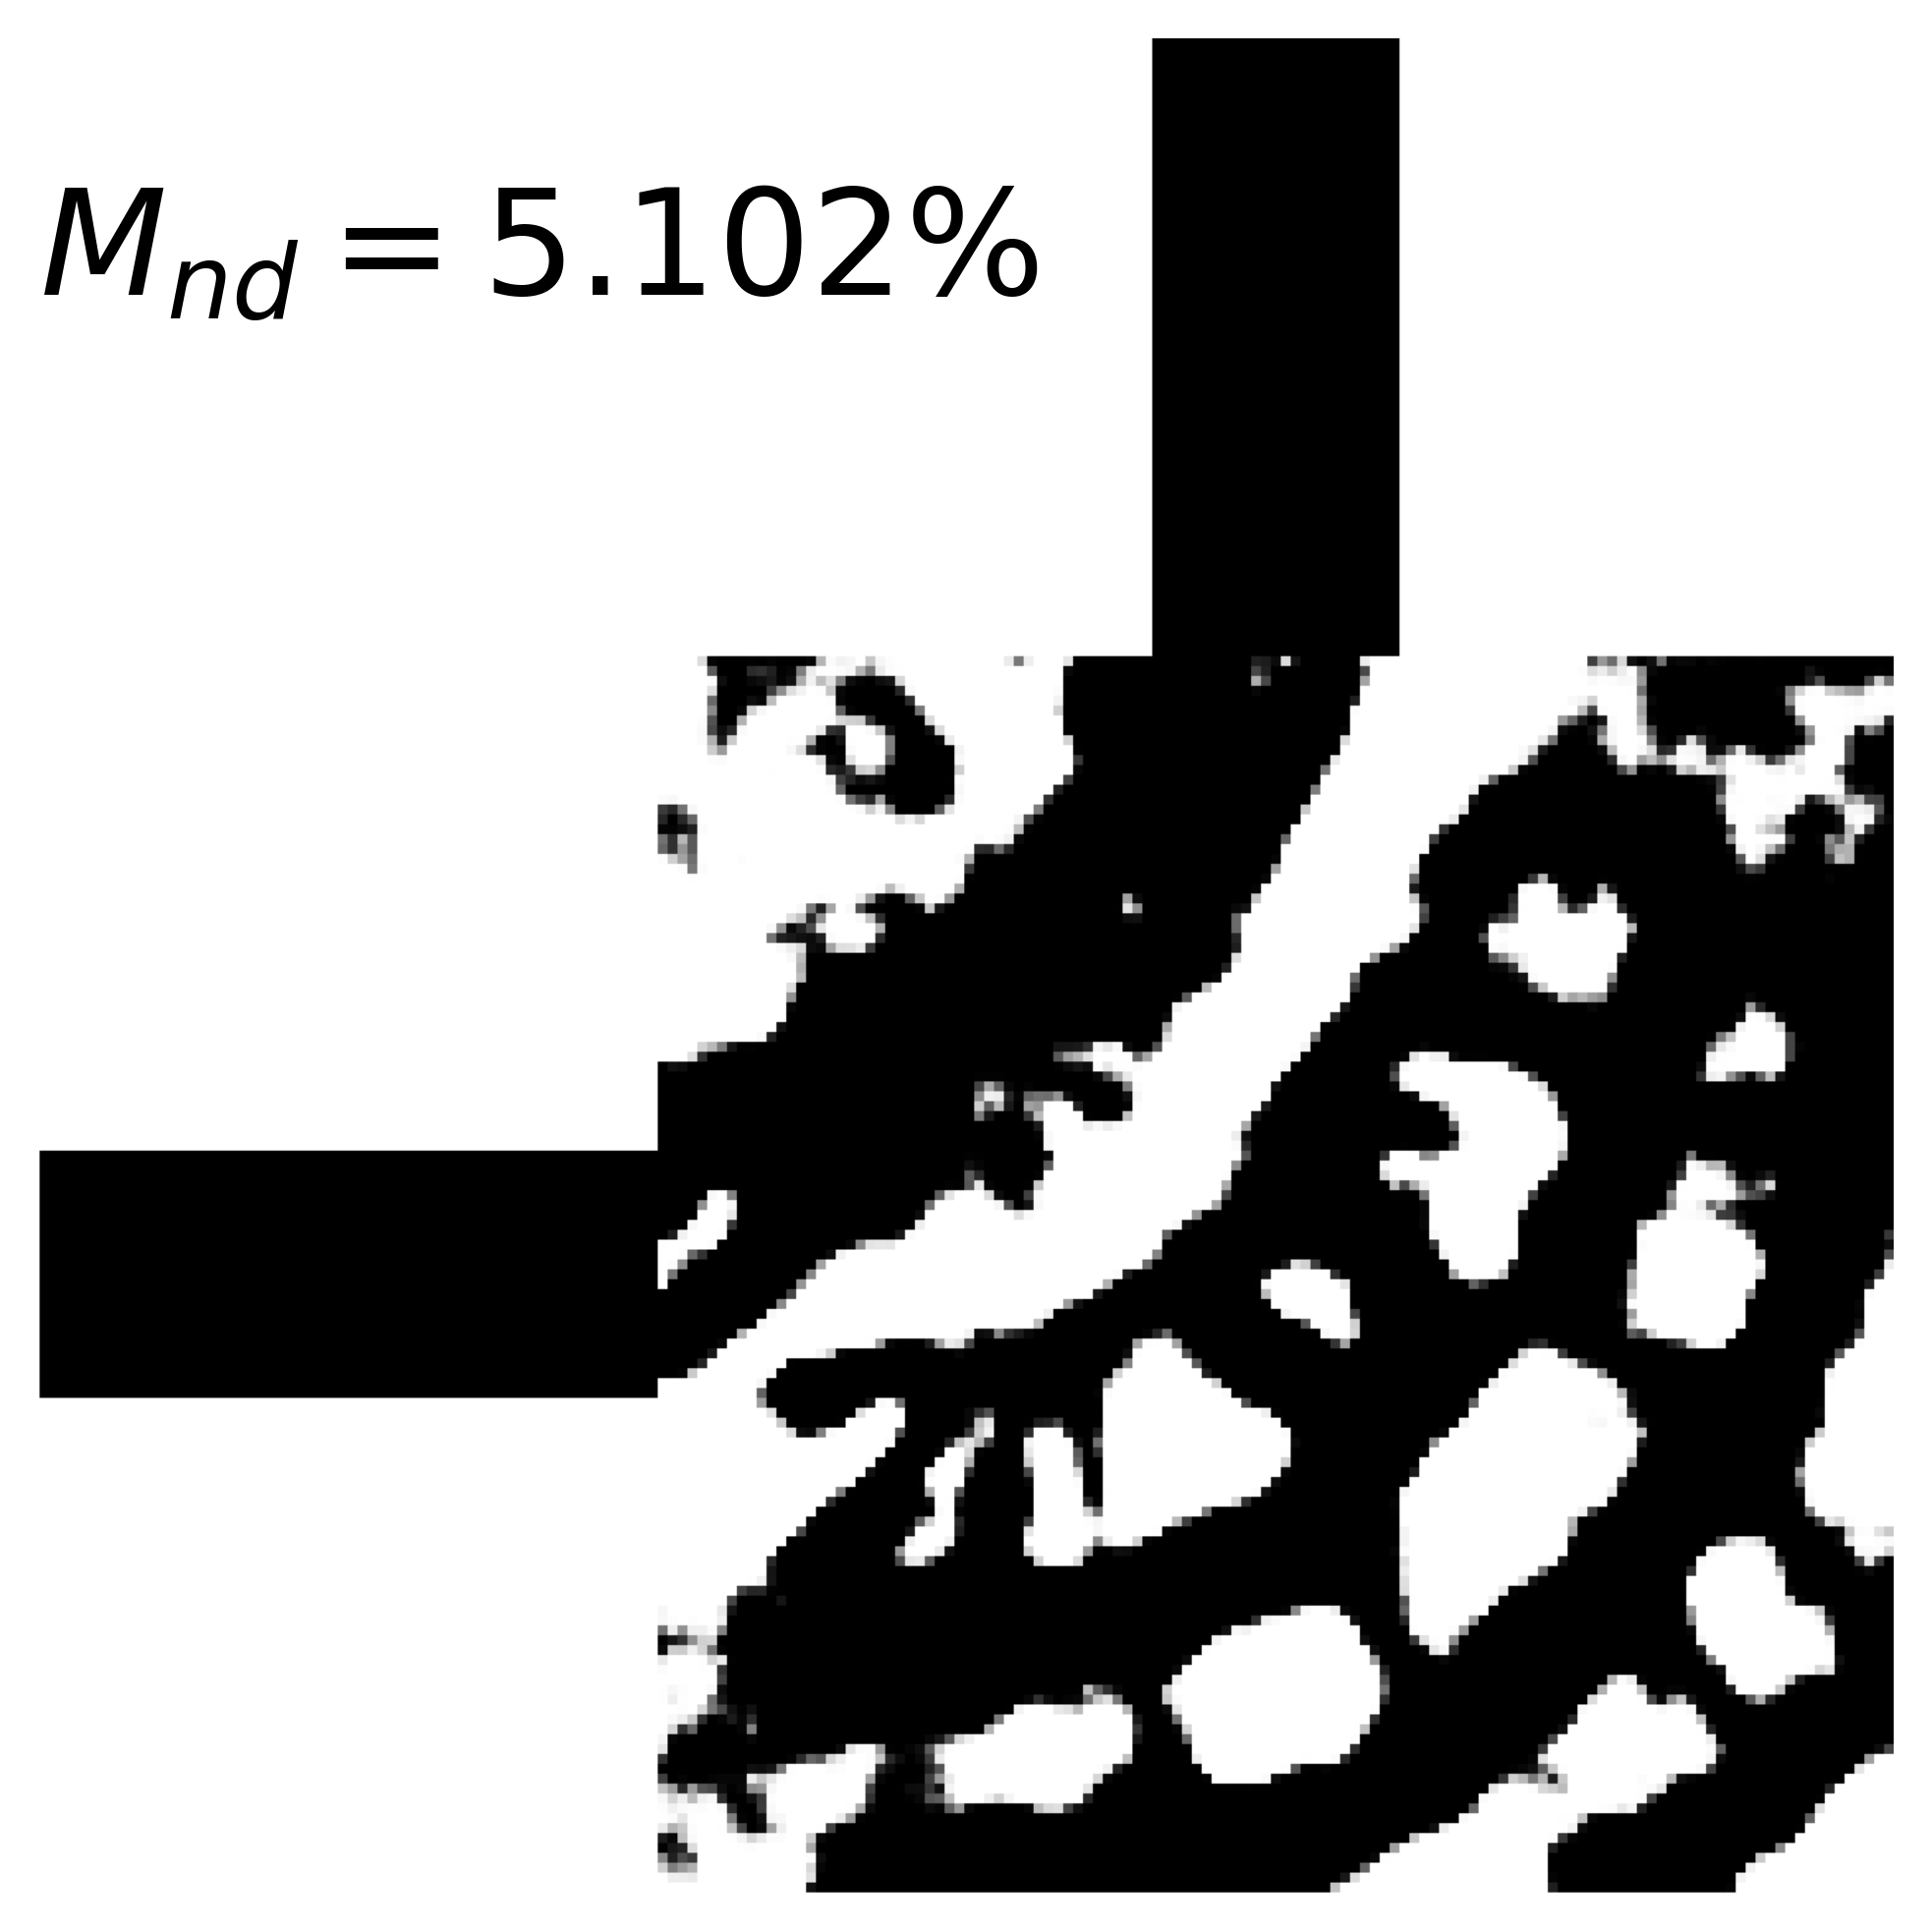
\includegraphics[width=0.20\textwidth]{image/results/bend/CMA-ES/visualize_eps_fab_256.png} \\
      \cline{2-4}
      &
      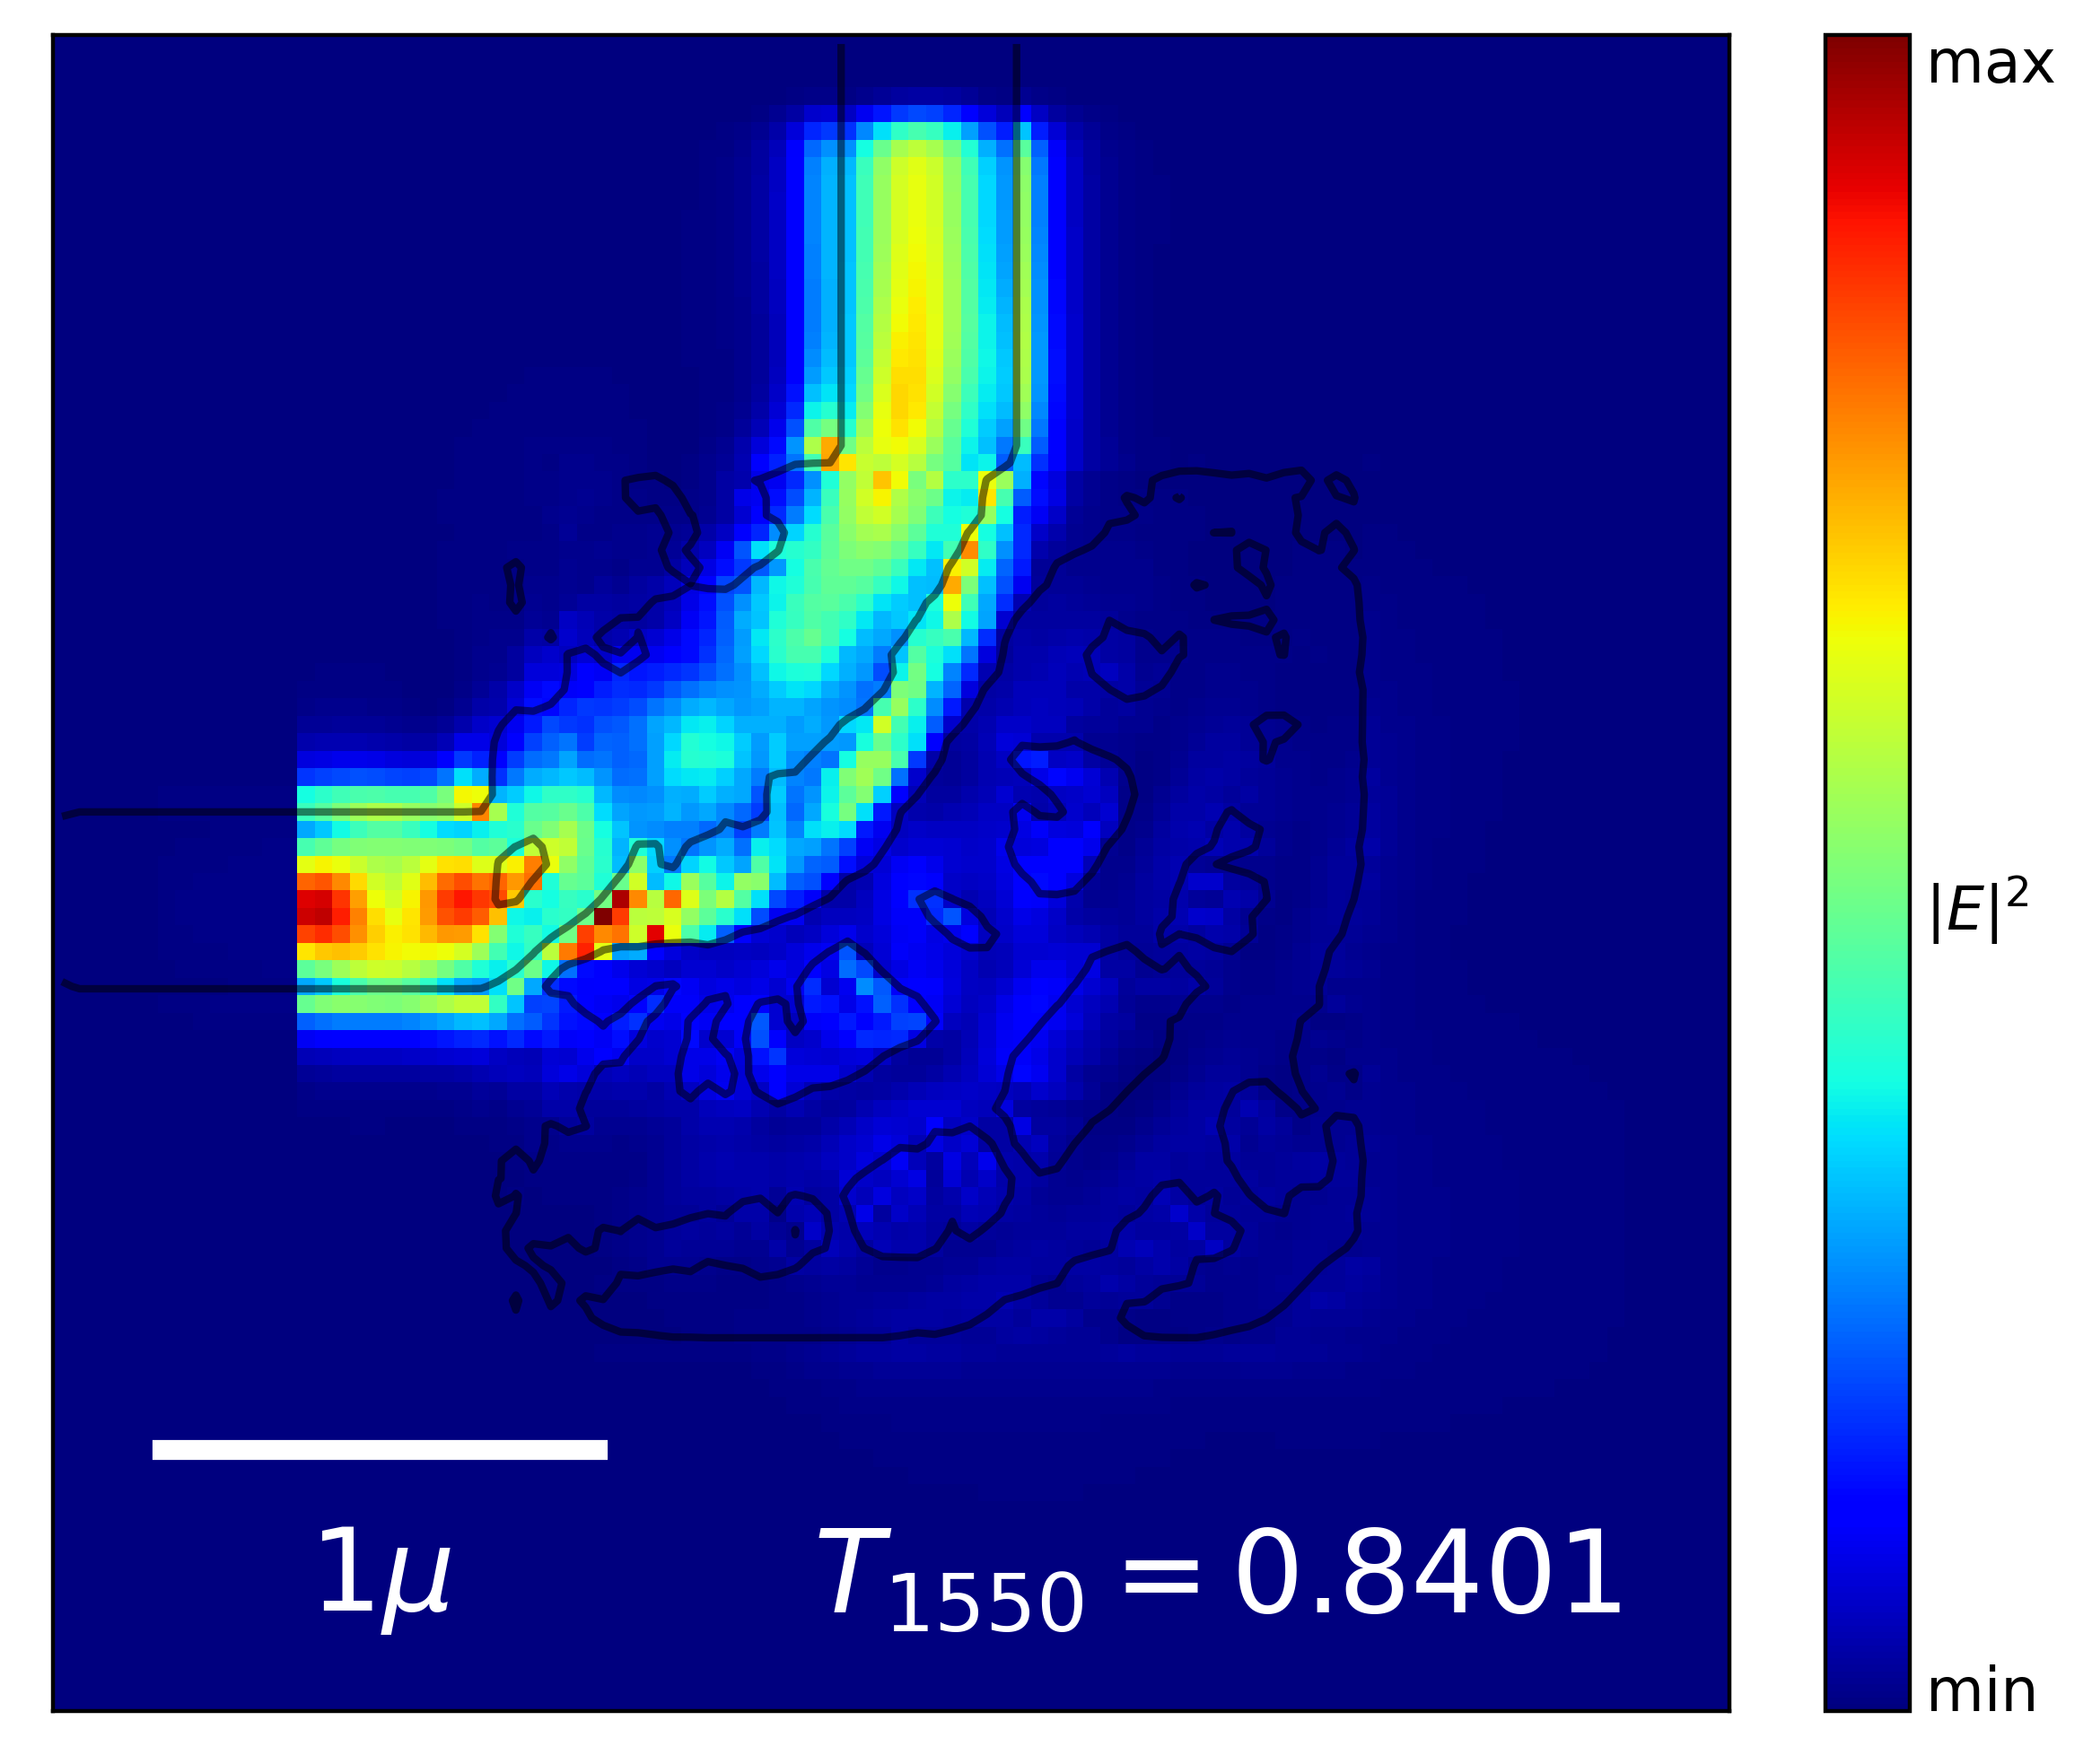
\includegraphics[width=0.33\textwidth]{image/results/bend/CMA-ES/visualize_field_cont_256.png} &
      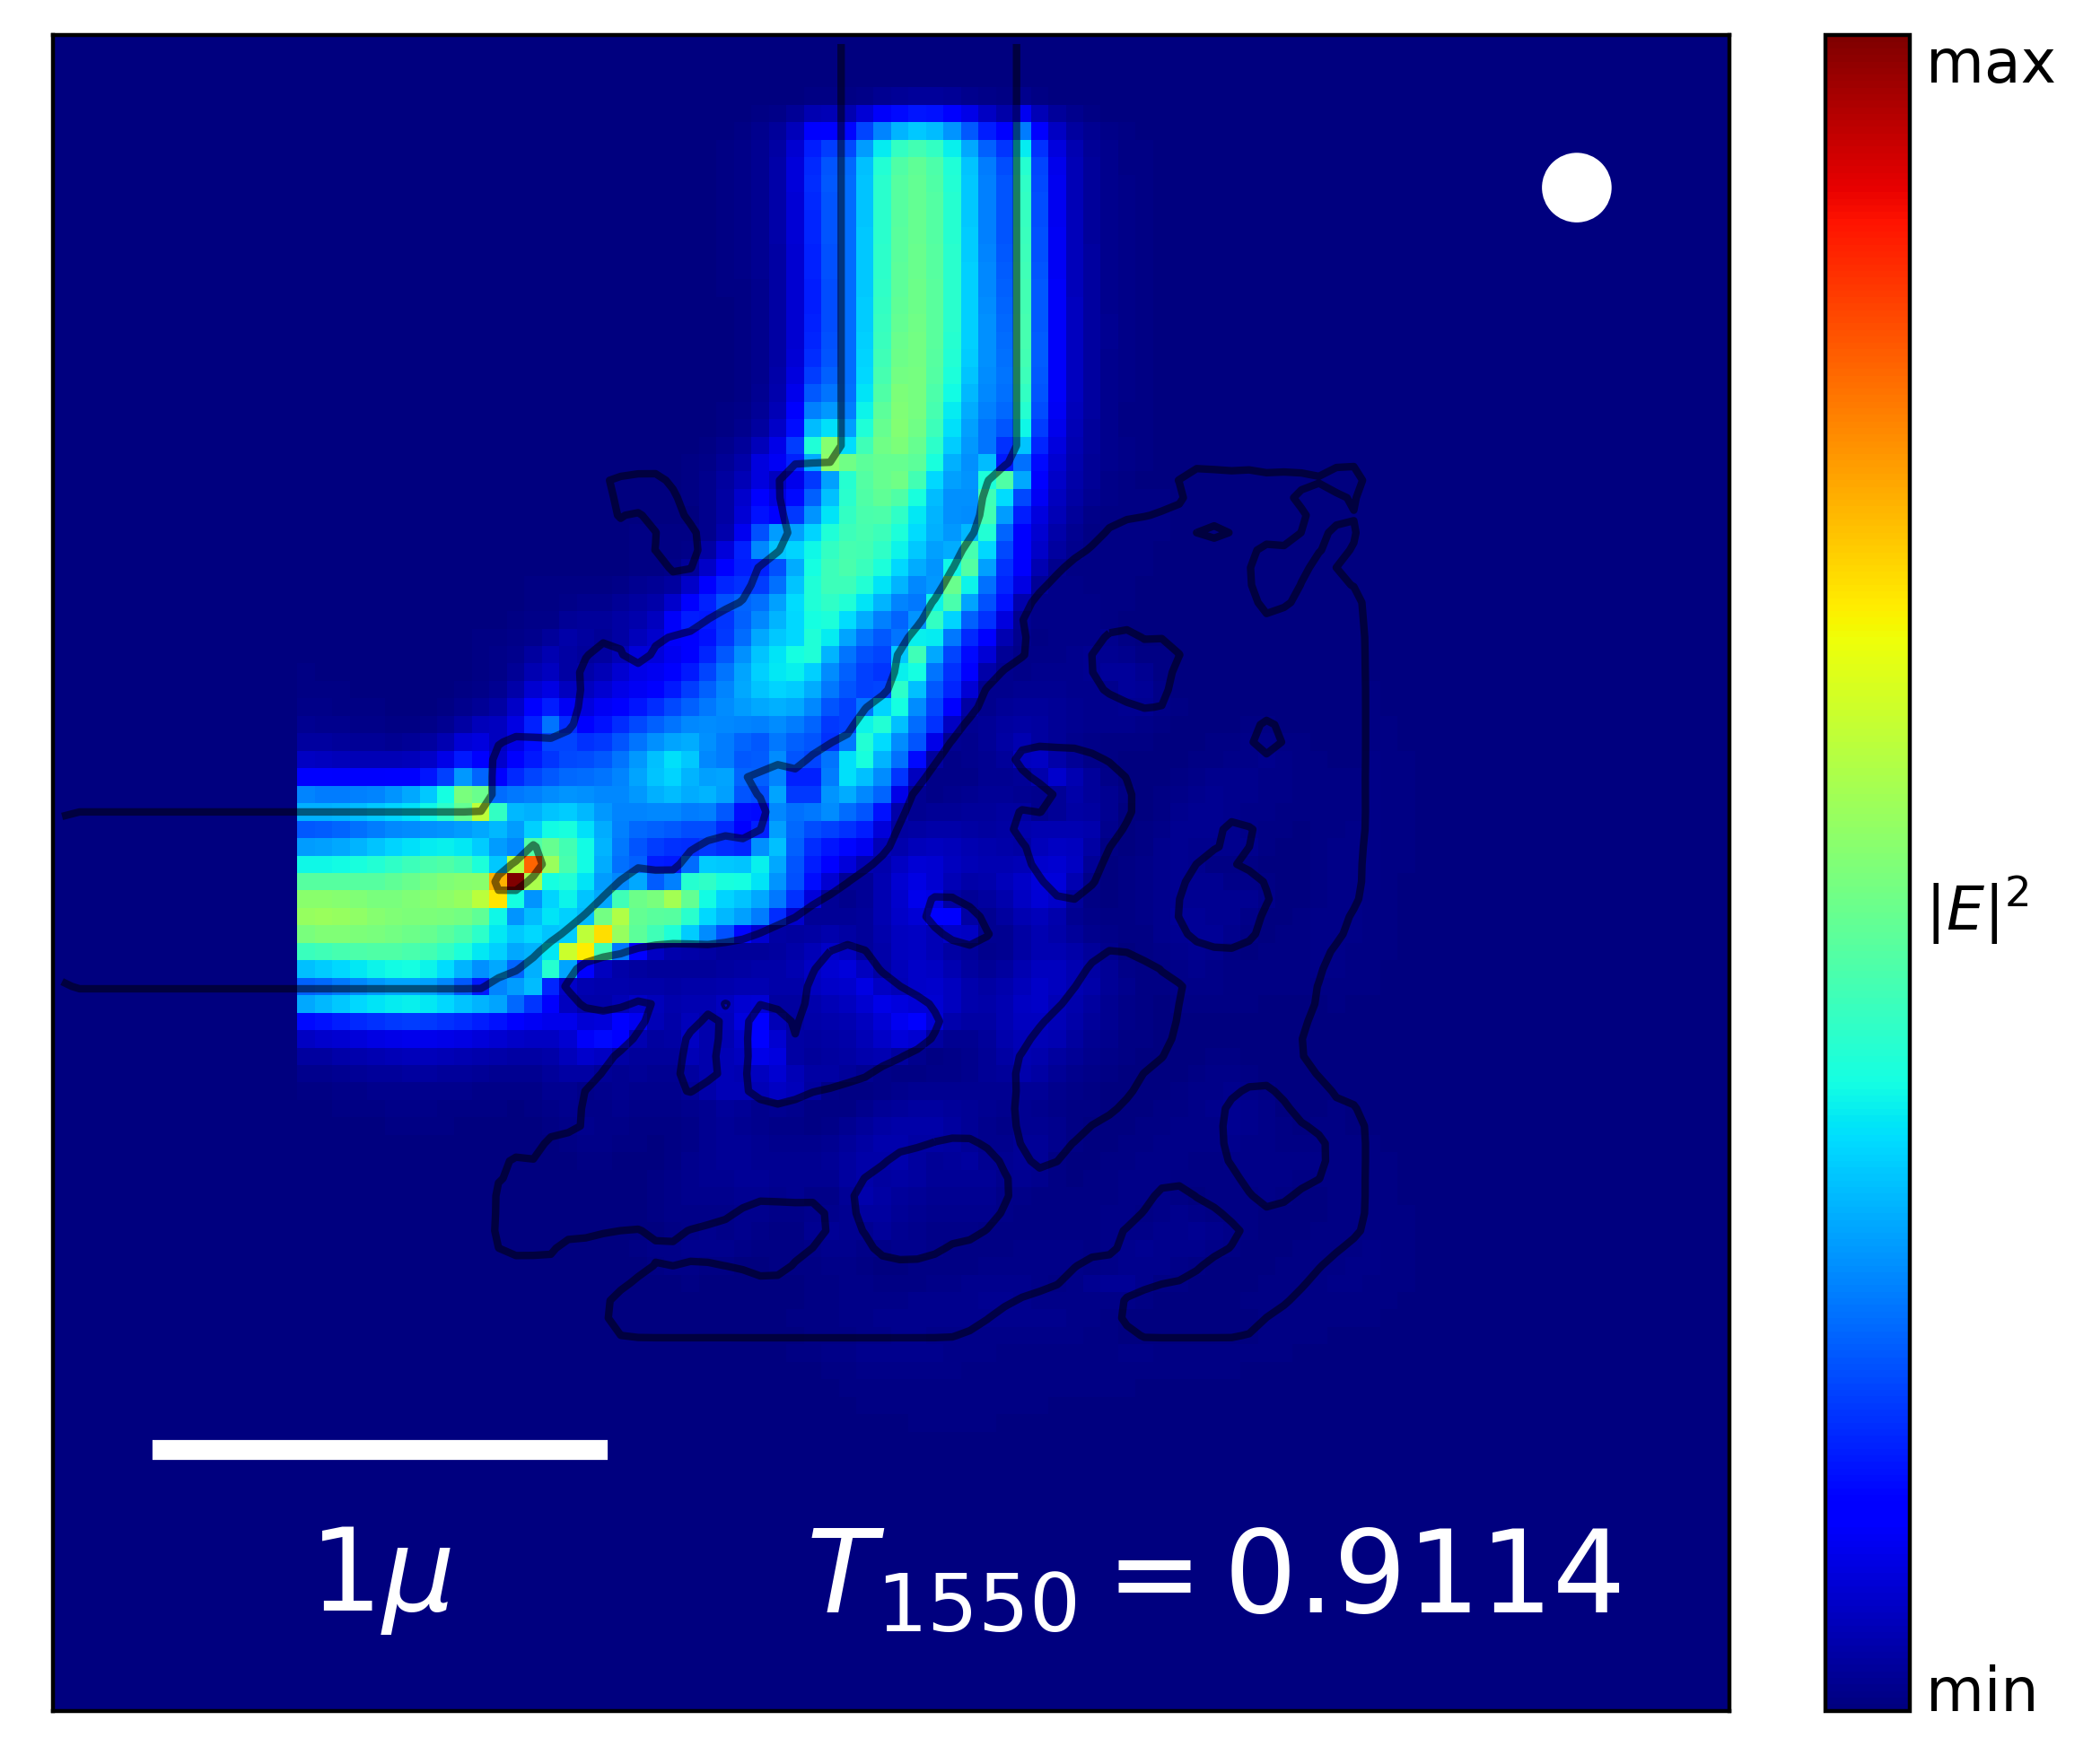
\includegraphics[width=0.33\textwidth]{image/results/bend/CMA-ES/visualize_field_disc_256.png} &
      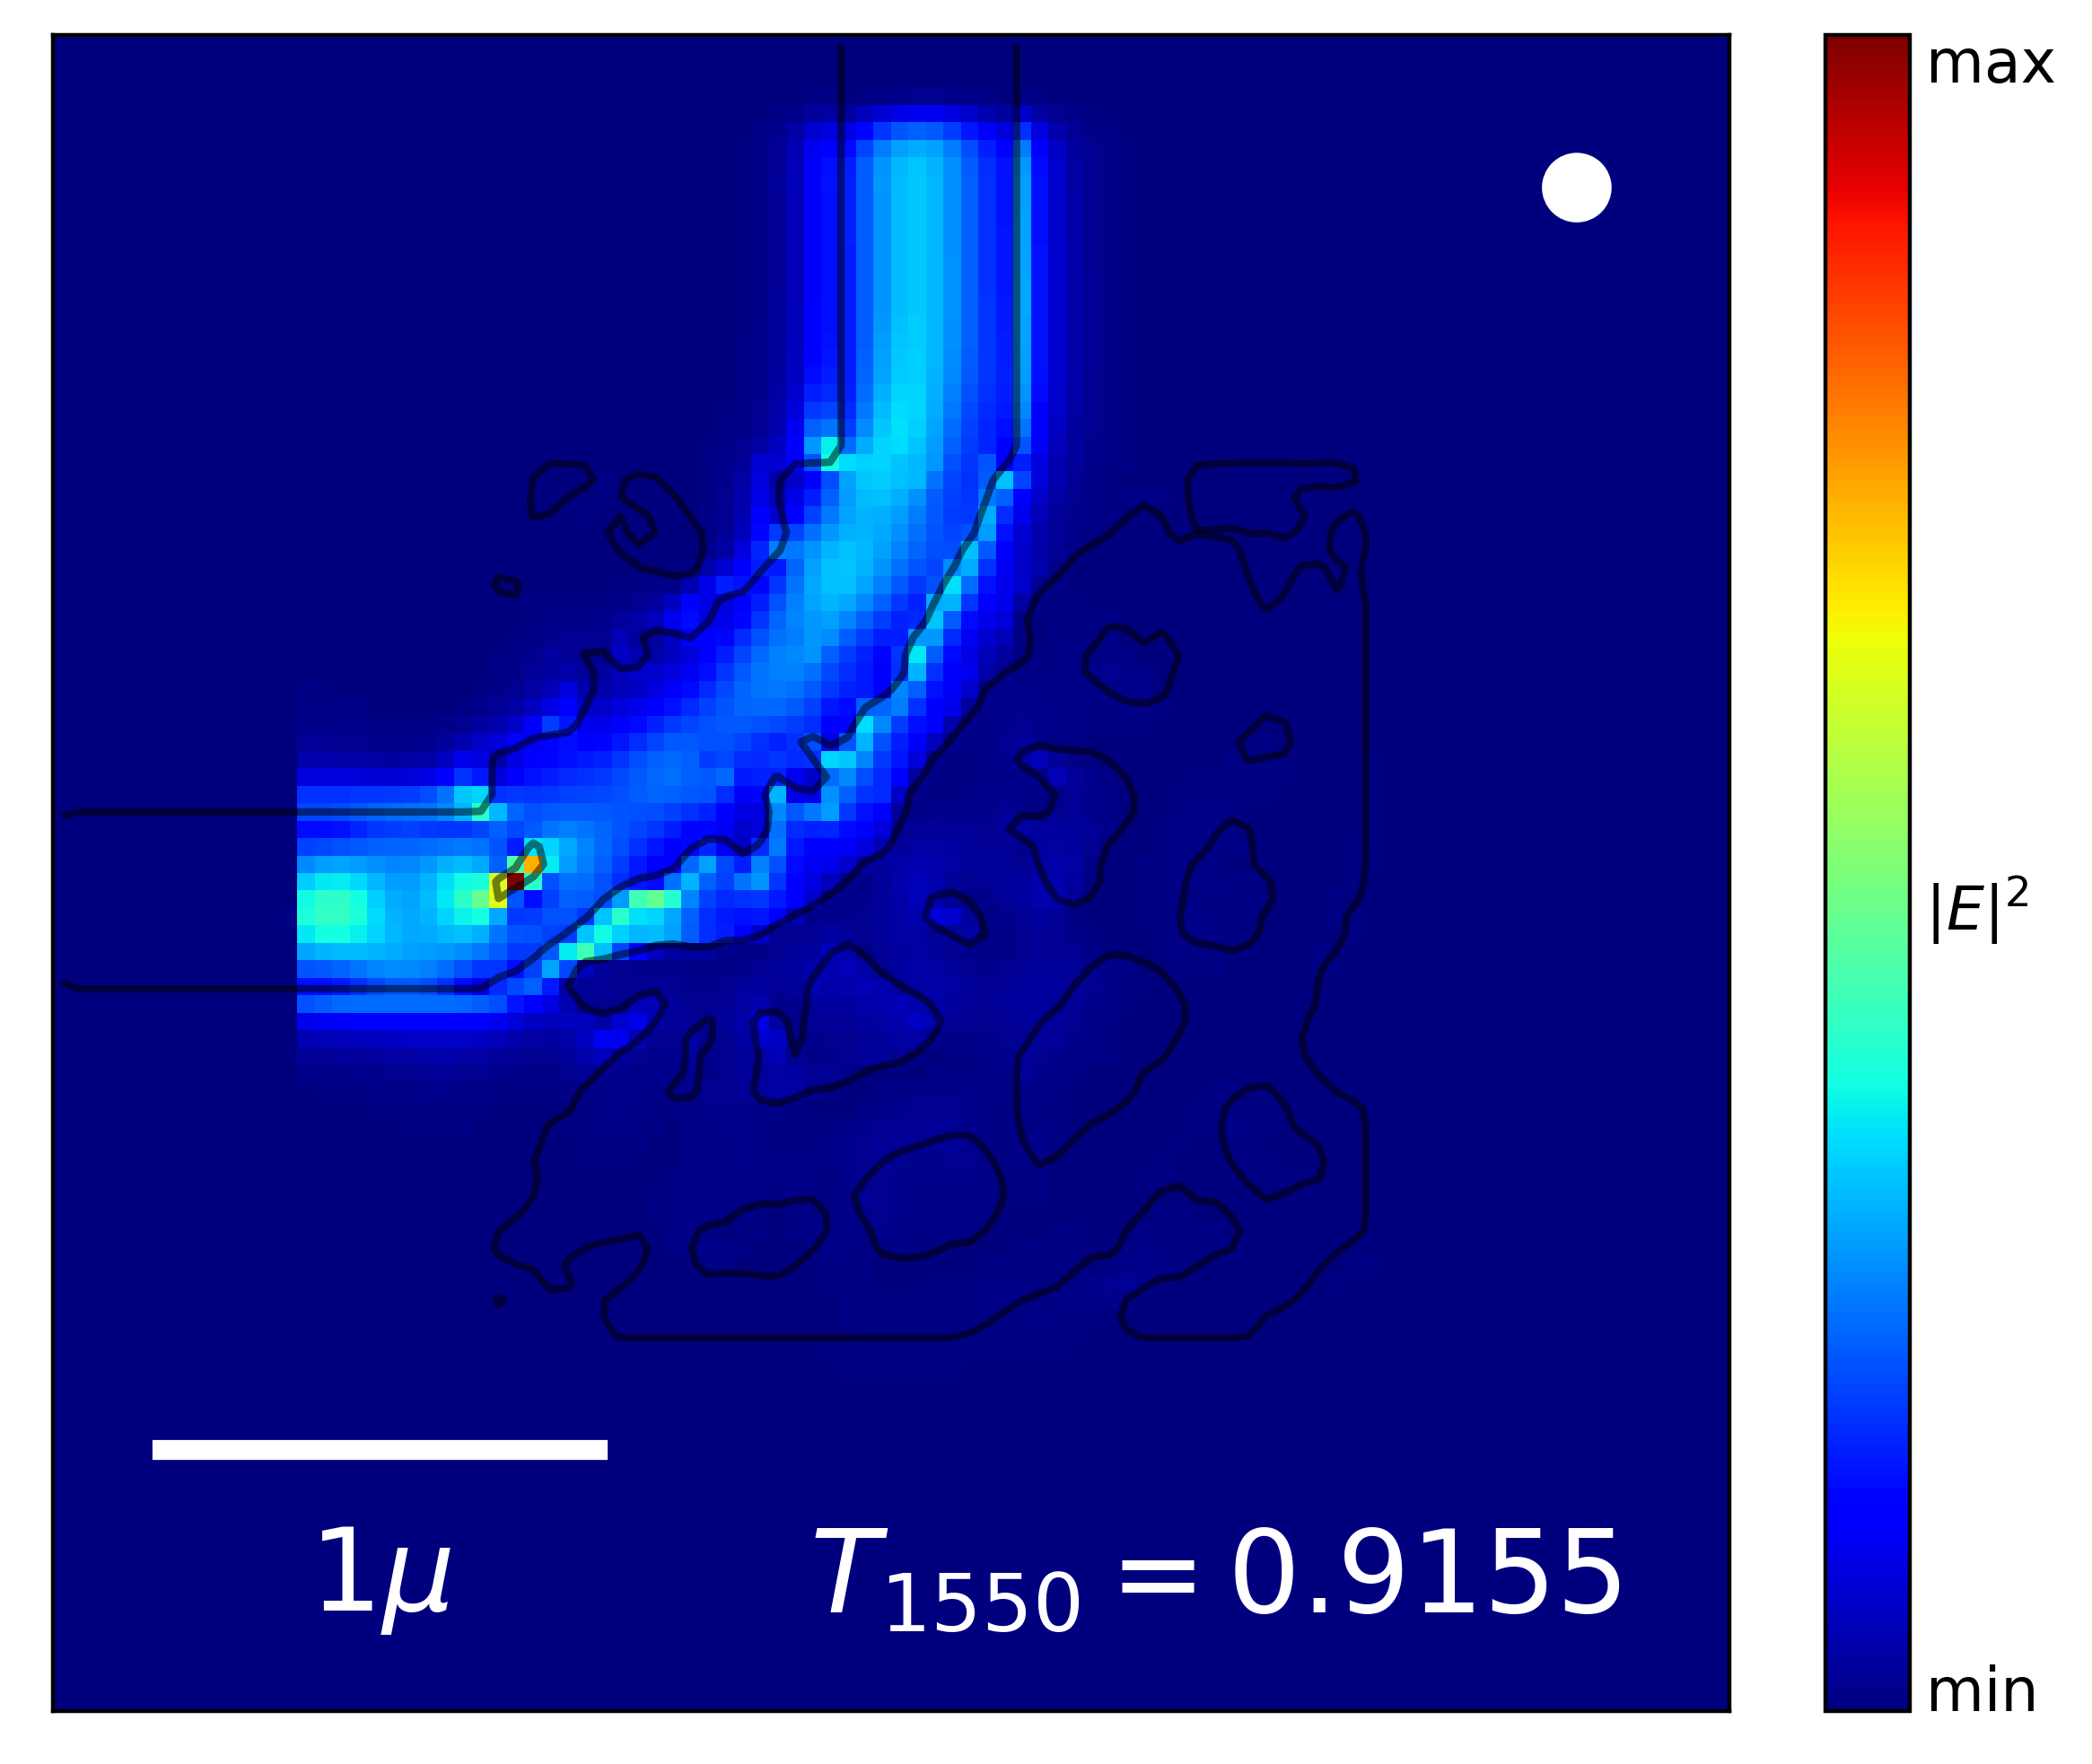
\includegraphics[width=0.33\textwidth]{image/results/bend/CMA-ES/visualize_field_fab_256.png} \\
    \hline
      \multirow{2}{*}{512} &
      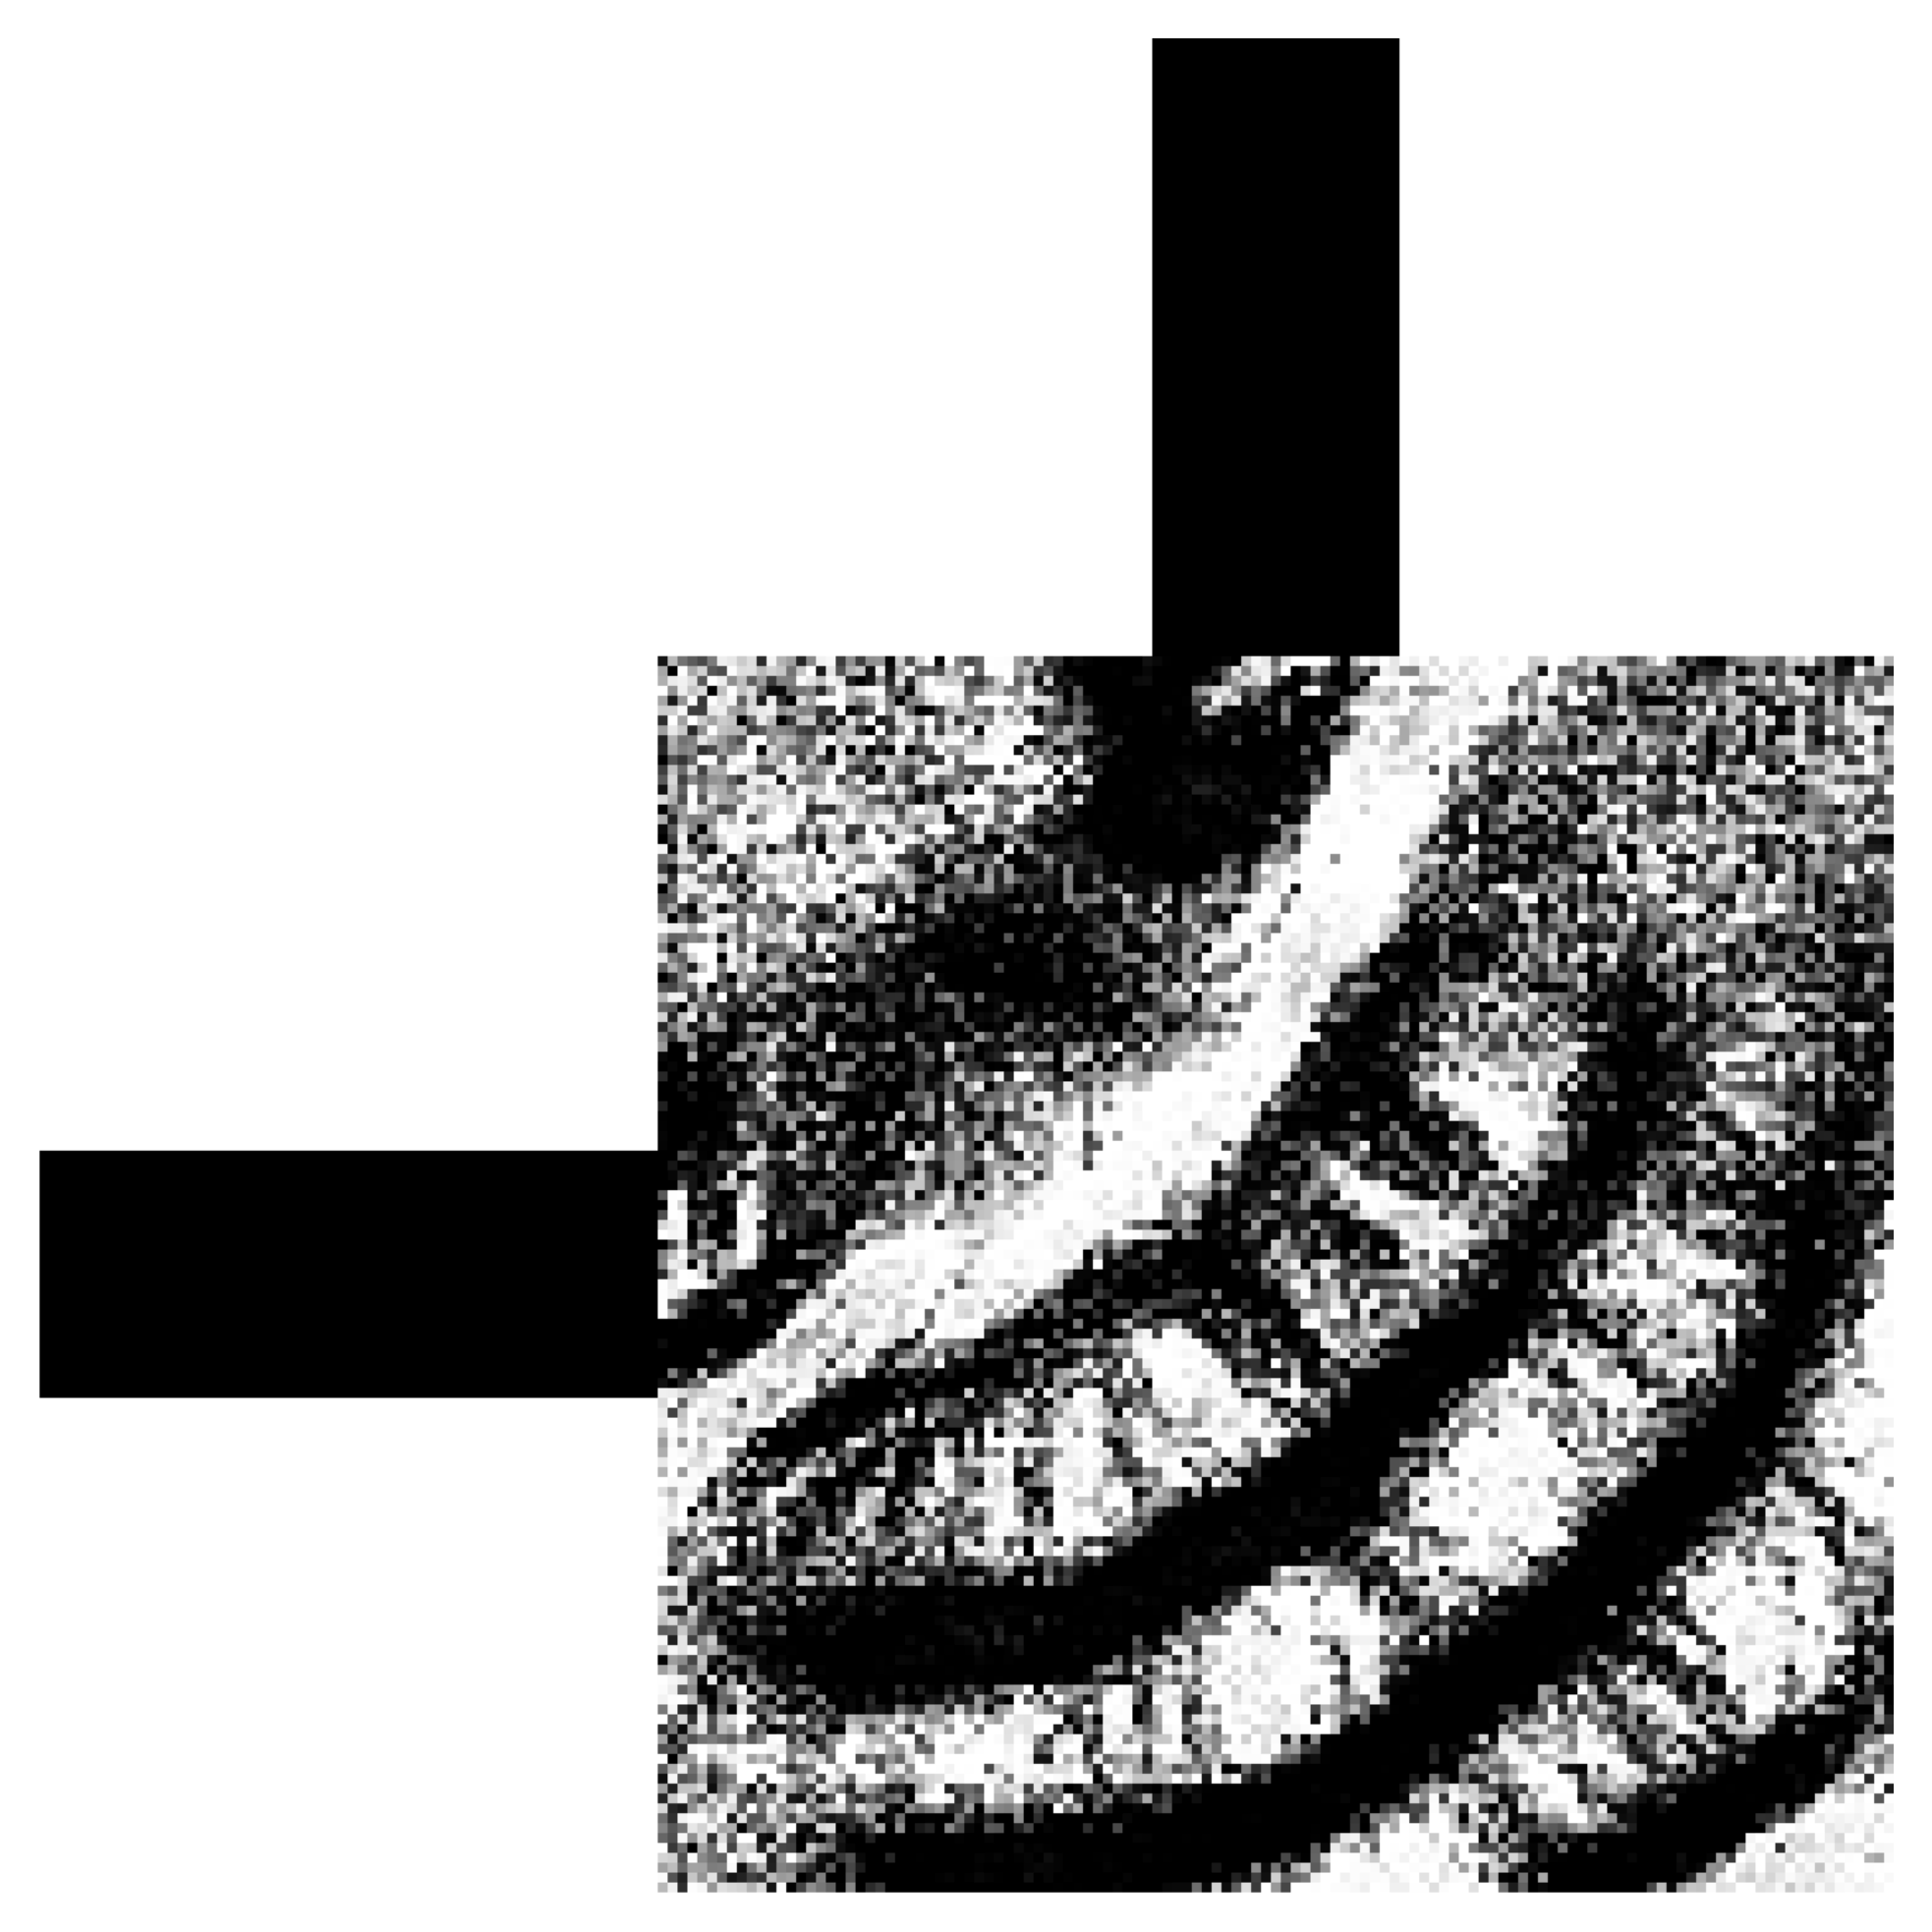
\includegraphics[width=0.20\textwidth]{image/results/bend/CMA-ES/visualize_eps_cont_512.png} &
      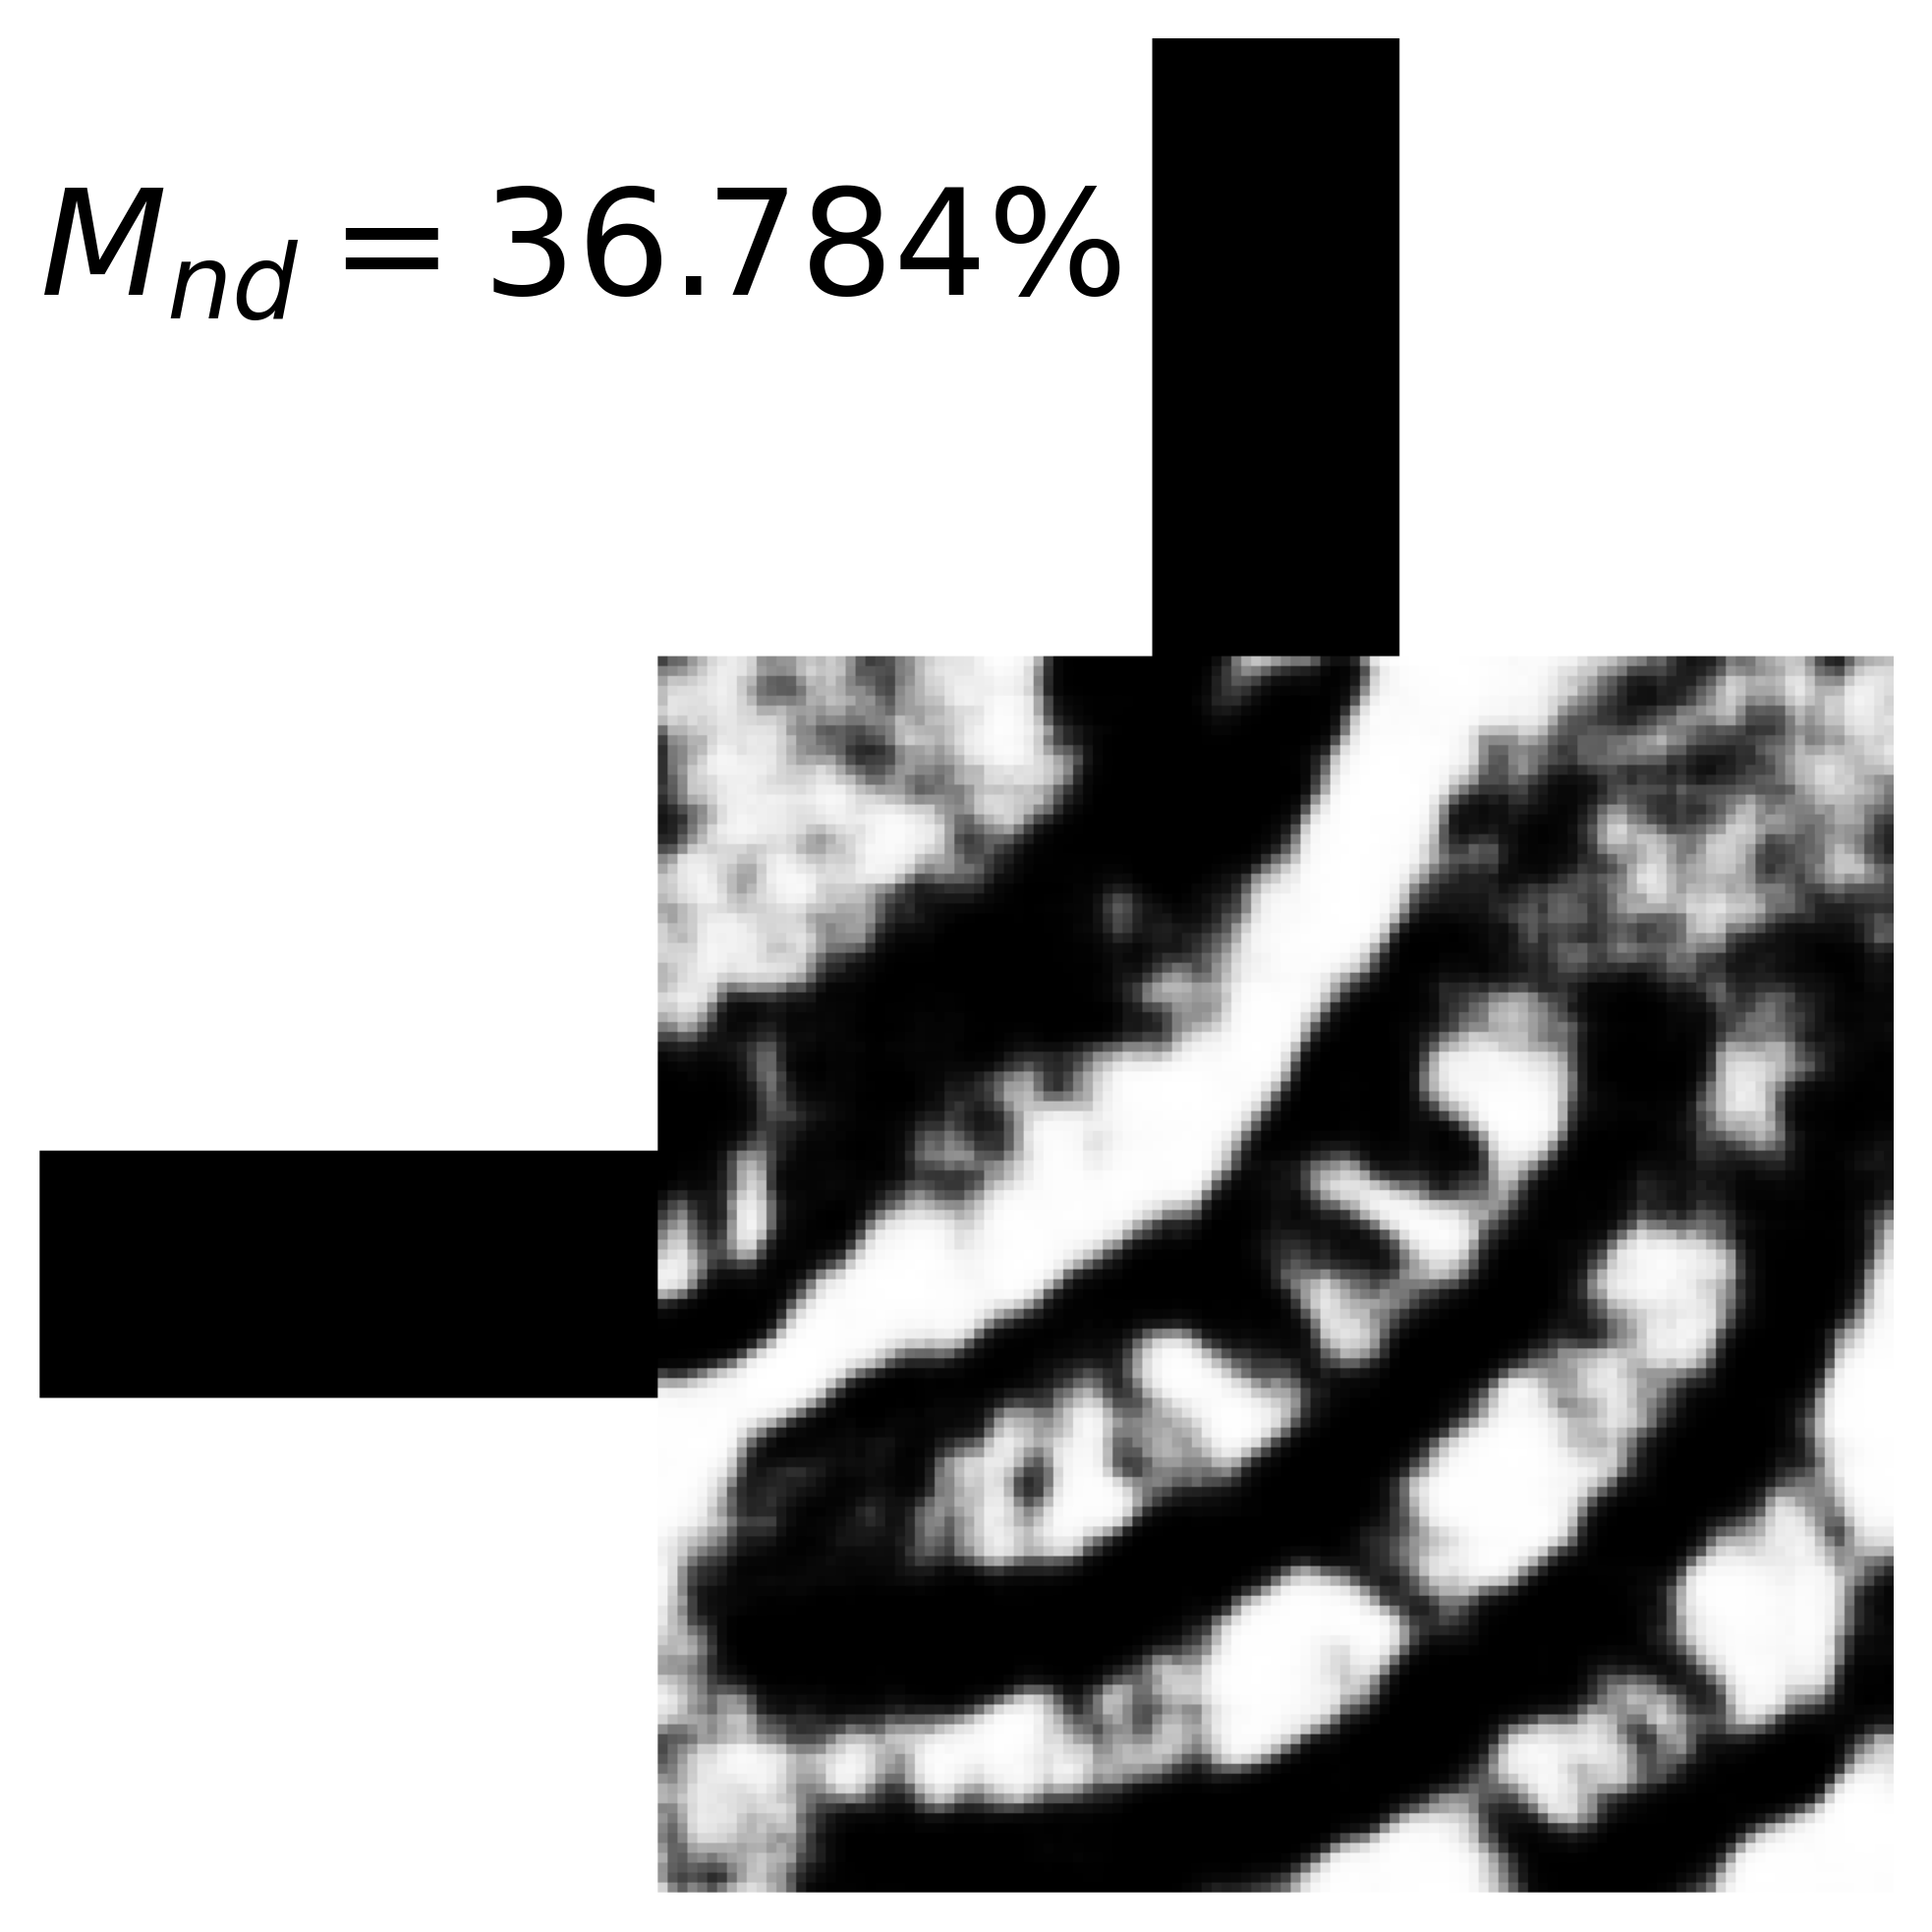
\includegraphics[width=0.20\textwidth]{image/results/bend/CMA-ES/visualize_eps_disc_512.png} &
      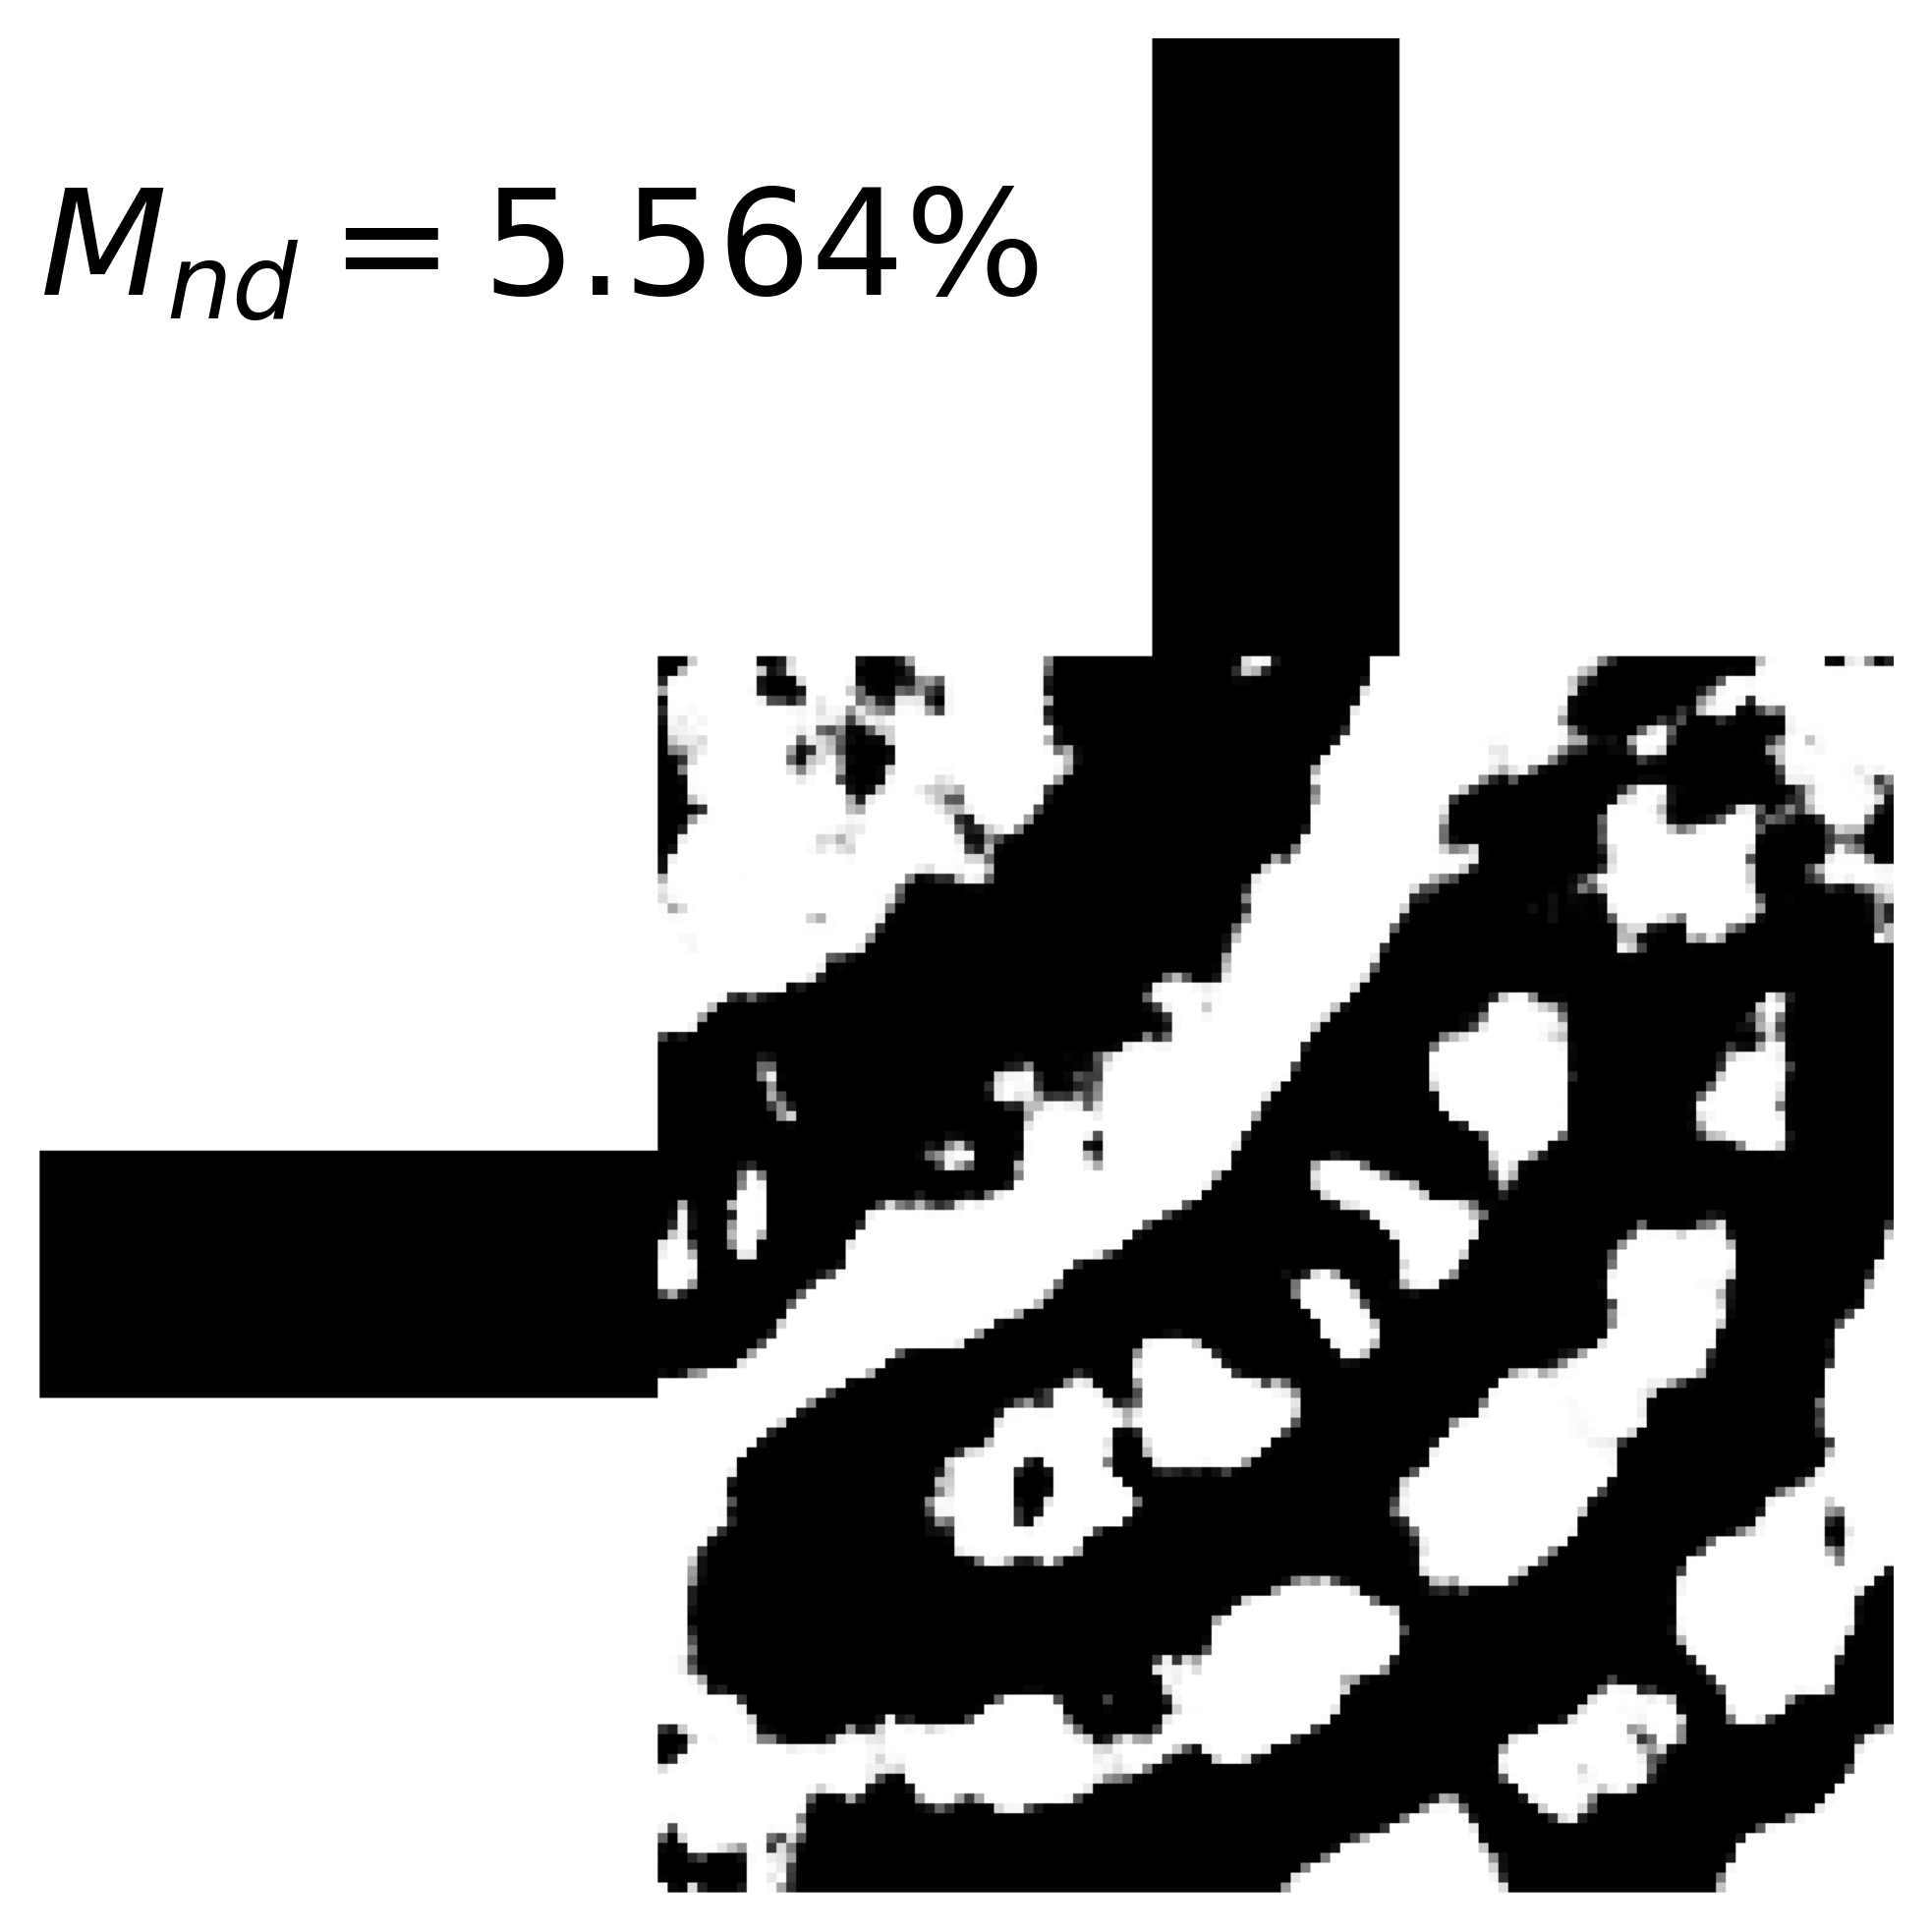
\includegraphics[width=0.20\textwidth]{image/results/bend/CMA-ES/visualize_eps_fab_512.png} \\
      \cline{2-4}
      &
      \includegraphics[width=0.33\textwidth]{image/results/bend/CMA-ES/visualize_field_cont_512.png} &
      \includegraphics[width=0.33\textwidth]{image/results/bend/CMA-ES/visualize_field_disc_512.png} &
      \includegraphics[width=0.33\textwidth]{image/results/bend/CMA-ES/visualize_field_fab_512.png} \\
    \hline
    \end{tabular}
    \hspace*{-3cm}
    \caption{Resultados de optimizar el \emph{bend} usando G-CMA-ES.}
    \label{tab:opt-CMA-bend}
\end{table}

% Bend - MMA
\begin{table}[ht]
    \centering
    \vspace*{-2.5cm}
    \hspace*{-3cm}
    \begin{tabular}{|c|c|c|c|}
    \hline 
    \emph{Seed} & Opt. continua & Opt. discreta &  Opt. de fabricación \\
    \hline
      %\multirow{2}{*}{128} &
      %\includegraphics[width=0.20\textwidth]{image/results/bend/MMA/visualize_eps_cont_128.png} &
      %\includegraphics[width=0.20\textwidth]{image/results/bend/MMA/visualize_eps_disc_128.png} &
      %\includegraphics[width=0.20\textwidth]{image/results/bend/MMA/visualize_eps_fab_128.png} \\
      %\cline{2-4}
      %&
      %\includegraphics[width=0.33\textwidth]{image/results/bend/MMA/visualize_field_cont_128.png} &
      %\includegraphics[width=0.33\textwidth]{image/results/bend/MMA/visualize_field_disc_128.png} &
      %\includegraphics[width=0.33\textwidth]{image/results/bend/MMA/visualize_field_fab_128.png} \\
    %\hline
      \multirow{2}{*}{256} &
      \includegraphics[width=0.20\textwidth]{image/results/bend/MMA/visualize_eps_cont_256.png} &
      \includegraphics[width=0.20\textwidth]{image/results/bend/MMA/visualize_eps_disc_256.png} &
      \includegraphics[width=0.20\textwidth]{image/results/bend/MMA/visualize_eps_fab_256.png} \\
      \cline{2-4}
      &
      \includegraphics[width=0.33\textwidth]{image/results/bend/MMA/visualize_field_cont_256.png} &
      \includegraphics[width=0.33\textwidth]{image/results/bend/MMA/visualize_field_disc_256.png} &
      \includegraphics[width=0.33\textwidth]{image/results/bend/MMA/visualize_field_fab_256.png} \\
    \hline
      \multirow{2}{*}{512} &
      \includegraphics[width=0.20\textwidth]{image/results/bend/MMA/visualize_eps_cont_512.png} &
      \includegraphics[width=0.20\textwidth]{image/results/bend/MMA/visualize_eps_disc_512.png} &
      \includegraphics[width=0.20\textwidth]{image/results/bend/MMA/visualize_eps_fab_512.png} \\
      \cline{2-4}
      &
      \includegraphics[width=0.33\textwidth]{image/results/bend/MMA/visualize_field_cont_512.png} &
      \includegraphics[width=0.33\textwidth]{image/results/bend/MMA/visualize_field_disc_512.png} &
      \includegraphics[width=0.33\textwidth]{image/results/bend/MMA/visualize_field_fab_512.png} \\
    \hline
    \end{tabular}
    \hspace*{-3cm}
    \caption{Resultados de optimizar el \emph{bend} usando MMA.}
    \label{tab:opt-MMA-bend}
\end{table}

% Bend - PSO
\begin{table}[ht]
    \centering
    \vspace*{-2.5cm}
    \hspace*{-3cm}
    \begin{tabular}{|c|c|c|c|}
    \hline 
    \emph{Seed} & Opt. continua & Opt. discreta &  Opt. de fabricación \\
    \hline
      \multirow{2}{*}{128} &
      \includegraphics[width=0.20\textwidth]{image/results/bend/PSO/visualize_eps_cont_128.png} &
      \includegraphics[width=0.20\textwidth]{image/results/bend/PSO/visualize_eps_disc_128.png} &
      \includegraphics[width=0.20\textwidth]{image/results/bend/PSO/visualize_eps_fab_128.png} \\
      \cline{2-4}
      &
      \includegraphics[width=0.33\textwidth]{image/results/bend/PSO/visualize_field_cont_128.png} &
      \includegraphics[width=0.33\textwidth]{image/results/bend/PSO/visualize_field_disc_128.png} &
      \includegraphics[width=0.33\textwidth]{image/results/bend/PSO/visualize_field_fab_128.png} \\
    \hline
      \multirow{2}{*}{256} &
      \includegraphics[width=0.20\textwidth]{image/results/bend/PSO/visualize_eps_cont_256.png} &
      \includegraphics[width=0.20\textwidth]{image/results/bend/PSO/visualize_eps_disc_256.png} \\
      %\includegraphics[width=0.20\textwidth]{image/results/bend/PSO/visualize_eps_fab_256.png} \\
      \cline{2-4}
      &
      \includegraphics[width=0.33\textwidth]{image/results/bend/PSO/visualize_field_cont_256.png} &
      \includegraphics[width=0.33\textwidth]{image/results/bend/PSO/visualize_field_disc_256.png} \\
      %\includegraphics[width=0.33\textwidth]{image/results/bend/PSO/visualize_field_fab_256.png} \\
    \hline
      \multirow{2}{*}{512} &
      \includegraphics[width=0.20\textwidth]{image/results/bend/PSO/visualize_eps_cont_512.png} &
      \includegraphics[width=0.20\textwidth]{image/results/bend/PSO/visualize_eps_disc_512.png} \\
      %\includegraphics[width=0.20\textwidth]{image/results/bend/PSO/visualize_eps_fab_512.png} \\
      \cline{2-4}
      &
      \includegraphics[width=0.33\textwidth]{image/results/bend/PSO/visualize_field_cont_512.png} &
      \includegraphics[width=0.33\textwidth]{image/results/bend/PSO/visualize_field_disc_512.png} \\
      %\includegraphics[width=0.33\textwidth]{image/results/bend/PSO/visualize_field_fab_512.png} \\
    \hline
    \end{tabular}
    \hspace*{-3cm}
    \caption{Resultados de optimizar el \emph{bend} usando G-PSO.}
    \label{tab:opt-PSO-bend}
\end{table}


% Bend - GA
\begin{table}[ht]
    \centering
    \vspace*{-2.5cm}
    \hspace*{-3cm}
    \begin{tabular}{|c|c|c|c|}
    \hline 
    \emph{Seed} & Opt. continua & Opt. discreta &  Opt. de fabricación \\
    \hline
      \multirow{2}{*}{128} &
      \includegraphics[width=0.20\textwidth]{image/results/bend/GA/visualize_eps_cont_128.png} &
      \includegraphics[width=0.20\textwidth]{image/results/bend/GA/visualize_eps_disc_128.png} &
      \includegraphics[width=0.20\textwidth]{image/results/bend/GA/visualize_eps_fab_128.png} \\
      \cline{2-4}
      &
      \includegraphics[width=0.33\textwidth]{image/results/bend/GA/visualize_field_cont_128.png} &
      \includegraphics[width=0.33\textwidth]{image/results/bend/GA/visualize_field_disc_128.png} &
      \includegraphics[width=0.33\textwidth]{image/results/bend/GA/visualize_field_fab_128.png} \\
    \hline
      \multirow{2}{*}{256} &
      \includegraphics[width=0.20\textwidth]{image/results/bend/GA/visualize_eps_cont_256.png} \\
      %\includegraphics[width=0.20\textwidth]{image/results/bend/GA/visualize_eps_disc_256.png} \\
      %\includegraphics[width=0.20\textwidth]{image/results/bend/GA/visualize_eps_fab_256.png} \\
      \cline{2-4}
      &
      \includegraphics[width=0.33\textwidth]{image/results/bend/GA/visualize_field_cont_256.png} \\
      %\includegraphics[width=0.33\textwidth]{image/results/bend/GA/visualize_field_disc_256.png} \\
      %\includegraphics[width=0.33\textwidth]{image/results/bend/GA/visualize_field_fab_256.png} \\
    \hline
      \multirow{2}{*}{512} &
      \includegraphics[width=0.20\textwidth]{image/results/bend/GA/visualize_eps_cont_512.png} \\
      %\includegraphics[width=0.20\textwidth]{image/results/bend/GA/visualize_eps_disc_512.png} \\
      %\includegraphics[width=0.20\textwidth]{image/results/bend/GA/visualize_eps_fab_512.png} \\
      \cline{2-4}
      &
      \includegraphics[width=0.33\textwidth]{image/results/bend/GA/visualize_field_cont_512.png} \\
      %\includegraphics[width=0.33\textwidth]{image/results/bend/GA/visualize_field_disc_512.png} \\
      %\includegraphics[width=0.33\textwidth]{image/results/bend/GA/visualize_field_fab_512.png} \\
    \hline
    \end{tabular}
    \hspace*{-3cm}
    \caption{Resultados de optimizar el \emph{bend} usando G-GA.}
    \label{tab:opt-GA-bend}
\end{table}

% \fi % FLAG

\section{Diseño del \emph{Bend} Mejor Optimizado}\label{sec:best-bend}

De la sección anterior tenemos que el \emph{bend} mejor optimizado se consiguió
utilizando el algoritmo L-BFGS-B con un \emph{seed} (valor de semilla) de 256.

Al aplicar la \autoref{eq:grayscale} obtenemos que el porcentage de región gris en el diseño
es de 1.097 \%, un valor menor a 2 \%, por lo cual podemos considerar que el diseño ha sido
correctamente binarizado. Por otro lado, si eliminamos las regiones no conectadas con la guía de entrada
tenemos un diseño con un porcentaje de gris de 0.168 \%.
Estos diseños lo podemos observar en la \autoref{fig:bestbend}.
Adicionalmente, en la \autoref{fig:broadband-bend} se muestra el comportamiento del diseño
en un rango de longitudes de onda de $1500nm$ a $1600 nm$.

\begin{figure}[ht]
  \centering

  % 1° row
  \subfigure[Diseño nominal.]
  {\includegraphics[width=0.45\textwidth]{image/results/bend/best/eps.png}}
  \hfill
  \subfigure[Diseño nominal tras eliminar regiones no conexas.]{
    \includegraphics[width=0.45\textwidth]{image/results/bend/best/eps_post.png}
  }

  % 2° row
  \subfigure[Campo $|\boldsymbol{E}|^2$ del diseño nominal.]
  {\includegraphics[width=0.45\textwidth]{image/results/bend/best/field.png}}
  \hfill
  \subfigure[Campo $|\boldsymbol{E}|^2$ del diseño nominal tras eliminar regiones no conexas.]{
    \includegraphics[width=0.45\textwidth]{image/results/bend/best/field_post.png}
  }

  \caption{Posprocesamiento del diseño del \emph{bend} mejor optimizado.}
  \label{fig:bestbend}

\end{figure}

\begin{figure}[ht]
  \centering
  \includegraphics[width=\textwidth]{image/results/bend/best/broadband-bend.png}
  \caption{Análisis del \emph{bend} mejor optimizado en un rango de longitudes de onda ($1500 nm-1600 nm$)}
  \label{fig:broadband-bend}
\end{figure}

\section{Resultados de Optimización del WDM}\label{sec:results-wdm}

%\iffalse % FLAG

En la \autoref{fig:wdm-cont}, \autoref{fig:wdm-disc} y \autoref{fig:wdm-fab} se observa 
el desempeño de los cinco algoritmos seleccionados en la etapa de optimización continua, discreta y
de fabricación del WDM, respectivamente.
Los resultados en más detalle por algoritmo se pueden encontrar en la
\autoref{tab:opt-LBFGSB-wdm} (L-BFGS-B),
\autoref{tab:opt-CMA-wdm} (G-CMA-ES),
\autoref{tab:opt-MMA-wdm} (MMA),
\autoref{tab:opt-PSO-wdm} (G-PSO) y
\autoref{tab:opt-GA-wdm} (G-GA).

\begin{landscape}
\begin{figure}[ht]
  \centering
  \includegraphics[scale=1.0]{image/results/wdm/wdm-opt-cont.png}
  \caption{Gráfico de valores de $f_{obj}$ obtenidos por los algoritmos en la optimización continua del WDM}
  \label{fig:wdm-cont}
\end{figure}
\end{landscape}

\begin{landscape}
\begin{figure}[ht]
  \centering
  \includegraphics[scale=1.0]{image/results/wdm/wdm-opt-disc.png}
  \caption{Gráfico de valores de $f_{obj}$ obtenidos por los algoritmos en la optimización discreta del WDM}
  \label{fig:wdm-disc}
\end{figure}
\end{landscape}

\begin{landscape}
\begin{figure}[ht]
  \centering
  \includegraphics[scale=1.0]{image/results/wdm/wdm-opt-fab.png}
  \caption{Gráfico de valores de $F_{obj}$ obtenidos por los algoritmos en la optimización de fabricación del WDM}
  \label{fig:wdm-fab}
\end{figure}
\end{landscape}


% WDM - L-BFGS-B
\begin{landscape}
\begin{table}[ht]
    \centering
    \vspace*{-2.5cm}
    \hspace*{-5cm}
    \begin{tabular}{|c|c|c|c|}
    \hline 
    \emph{Seed} & Opt. continua & Opt. discreta &  Opt. de fabricación \\
    \hline
      \multirow{2}{*}{128} &
      \includegraphics[width=0.24\textwidth]{image/results/wdm/L-BFGS-B/visualize_eps_cont_128.png} &
      \includegraphics[width=0.24\textwidth]{image/results/wdm/L-BFGS-B/visualize_eps_disc_128.png} &
      \includegraphics[width=0.24\textwidth]{image/results/wdm/L-BFGS-B/visualize_eps_fab_128.png} \\
      \cline{2-4}
      &
      \includegraphics[width=0.50\textwidth]{image/results/wdm/L-BFGS-B/visualize_field_cont_128.png} &
      \includegraphics[width=0.50\textwidth]{image/results/wdm/L-BFGS-B/visualize_field_disc_128.png} &
      \includegraphics[width=0.50\textwidth]{image/results/wdm/L-BFGS-B/visualize_field_fab_128.png} \\
    \hline
      \multirow{2}{*}{256} &
      \includegraphics[width=0.24\textwidth]{image/results/wdm/L-BFGS-B/visualize_eps_cont_256.png} &
      \includegraphics[width=0.24\textwidth]{image/results/wdm/L-BFGS-B/visualize_eps_disc_256.png} &
      \includegraphics[width=0.24\textwidth]{image/results/wdm/L-BFGS-B/visualize_eps_fab_256.png} \\
      \cline{2-4}
      &
      \includegraphics[width=0.50\textwidth]{image/results/wdm/L-BFGS-B/visualize_field_cont_256.png} &
      \includegraphics[width=0.50\textwidth]{image/results/wdm/L-BFGS-B/visualize_field_disc_256.png} &
      \includegraphics[width=0.50\textwidth]{image/results/wdm/L-BFGS-B/visualize_field_fab_256.png} \\
    \hline
      \multirow{2}{*}{512} &
      \includegraphics[width=0.24\textwidth]{image/results/wdm/L-BFGS-B/visualize_eps_cont_512.png} &
      \includegraphics[width=0.24\textwidth]{image/results/wdm/L-BFGS-B/visualize_eps_disc_512.png} &
      \includegraphics[width=0.24\textwidth]{image/results/wdm/L-BFGS-B/visualize_eps_fab_512.png} \\
      \cline{2-4}
      &
      \includegraphics[width=0.50\textwidth]{image/results/wdm/L-BFGS-B/visualize_field_cont_512.png} &
      \includegraphics[width=0.50\textwidth]{image/results/wdm/L-BFGS-B/visualize_field_disc_512.png} &
      \includegraphics[width=0.50\textwidth]{image/results/wdm/L-BFGS-B/visualize_field_fab_512.png} \\
    \hline
    \end{tabular}
    \hspace*{-5cm}
    \caption{Resultados de optimizar el WDM usando L-BFGS-B.}
    \label{tab:opt-LBFGSB-wdm}
\end{table}
\end{landscape}

% WDM - CMA
\begin{landscape}
\begin{table}[ht]
    \centering
    \vspace*{-2.5cm}
    \hspace*{-5cm}
    \begin{tabular}{|c|c|c|c|}
    \hline 
    \emph{Seed} & Opt. continua & Opt. discreta &  Opt. de fabricación \\
    \hline
      \multirow{2}{*}{128} &
      \includegraphics[width=0.24\textwidth]{image/results/wdm/CMA-ES/visualize_eps_cont_128.png} &
      \includegraphics[width=0.24\textwidth]{image/results/wdm/CMA-ES/visualize_eps_disc_128.png} &
      \includegraphics[width=0.24\textwidth]{image/results/wdm/CMA-ES/visualize_eps_fab_128.png} \\
      \cline{2-4}
      &
      \includegraphics[width=0.50\textwidth]{image/results/wdm/CMA-ES/visualize_field_cont_128.png} &
      \includegraphics[width=0.50\textwidth]{image/results/wdm/CMA-ES/visualize_field_disc_128.png} &
      \includegraphics[width=0.50\textwidth]{image/results/wdm/CMA-ES/visualize_field_fab_128.png} \\
    \hline
      \multirow{2}{*}{256} &
      \includegraphics[width=0.24\textwidth]{image/results/wdm/CMA-ES/visualize_eps_cont_256.png} &
      \includegraphics[width=0.24\textwidth]{image/results/wdm/CMA-ES/visualize_eps_disc_256.png} &
      \includegraphics[width=0.24\textwidth]{image/results/wdm/CMA-ES/visualize_eps_fab_256.png} \\
      \cline{2-4}
      &
      \includegraphics[width=0.50\textwidth]{image/results/wdm/CMA-ES/visualize_field_cont_256.png} &
      \includegraphics[width=0.50\textwidth]{image/results/wdm/CMA-ES/visualize_field_disc_256.png} &
      \includegraphics[width=0.50\textwidth]{image/results/wdm/CMA-ES/visualize_field_fab_256.png} \\
    \hline
      \multirow{2}{*}{512} &
      \includegraphics[width=0.24\textwidth]{image/results/wdm/CMA-ES/visualize_eps_cont_512.png} &
      \includegraphics[width=0.24\textwidth]{image/results/wdm/CMA-ES/visualize_eps_disc_512.png} &
      \includegraphics[width=0.24\textwidth]{image/results/wdm/CMA-ES/visualize_eps_fab_512.png} \\
      \cline{2-4}
      &
      \includegraphics[width=0.50\textwidth]{image/results/wdm/CMA-ES/visualize_field_cont_512.png} &
      \includegraphics[width=0.50\textwidth]{image/results/wdm/CMA-ES/visualize_field_disc_512.png} &
      \includegraphics[width=0.50\textwidth]{image/results/wdm/CMA-ES/visualize_field_fab_512.png} \\
    \hline
    \end{tabular}
    \hspace*{-5cm}
    \caption{Resultados de optimizar el WDM usando G-CMA-ES.}
    \label{tab:opt-CMA-wdm}
\end{table}
\end{landscape}

% WDM - MMA
\begin{landscape}
\begin{table}[ht]
    \centering
    \vspace*{-2.5cm}
    \hspace*{-5cm}
    \begin{tabular}{|c|c|c|c|}
    \hline 
    \emph{Seed} & Opt. continua & Opt. discreta &  Opt. de fabricación \\
    \hline
      %\multirow{2}{*}{128} &
      %\includegraphics[width=0.24\textwidth]{image/results/wdm/MMA/visualize_eps_cont_128.png} &
      %\includegraphics[width=0.24\textwidth]{image/results/wdm/MMA/visualize_eps_disc_128.png} &
      %\includegraphics[width=0.24\textwidth]{image/results/wdm/MMA/visualize_eps_fab_128.png} \\
      %\cline{2-4}
      %&
      %\includegraphics[width=0.50\textwidth]{image/results/wdm/MMA/visualize_field_cont_128.png} &
      %\includegraphics[width=0.50\textwidth]{image/results/wdm/MMA/visualize_field_disc_128.png} &
      %\includegraphics[width=0.50\textwidth]{image/results/wdm/MMA/visualize_field_fab_128.png} \\
    %\hline
      \multirow{2}{*}{256} &
      \includegraphics[width=0.24\textwidth]{image/results/wdm/MMA/visualize_eps_cont_256.png} &
      \includegraphics[width=0.24\textwidth]{image/results/wdm/MMA/visualize_eps_disc_256.png} &
      \includegraphics[width=0.24\textwidth]{image/results/wdm/MMA/visualize_eps_fab_256.png} \\
      \cline{2-4}
      &
      \includegraphics[width=0.50\textwidth]{image/results/wdm/MMA/visualize_field_cont_256.png} &
      \includegraphics[width=0.50\textwidth]{image/results/wdm/MMA/visualize_field_disc_256.png} &
      \includegraphics[width=0.50\textwidth]{image/results/wdm/MMA/visualize_field_fab_256.png} \\
    \hline
      \multirow{2}{*}{512} &
      \includegraphics[width=0.24\textwidth]{image/results/wdm/MMA/visualize_eps_cont_512.png} &
      \includegraphics[width=0.24\textwidth]{image/results/wdm/MMA/visualize_eps_disc_512.png} &
      \includegraphics[width=0.24\textwidth]{image/results/wdm/MMA/visualize_eps_fab_512.png} \\
      \cline{2-4}
      &
      \includegraphics[width=0.50\textwidth]{image/results/wdm/MMA/visualize_field_cont_512.png} &
      \includegraphics[width=0.50\textwidth]{image/results/wdm/MMA/visualize_field_disc_512.png} &
      \includegraphics[width=0.50\textwidth]{image/results/wdm/MMA/visualize_field_fab_512.png} \\
    \hline
    \end{tabular}
    \hspace*{-5cm}
    \caption{Resultados de optimizar el WDM usando MMA.}
    \label{tab:opt-MMA-wdm}
\end{table}
\end{landscape}

% WDM - PSO
\begin{landscape}
\begin{table}[ht]
    \centering
    \vspace*{-2.5cm}
    \hspace*{-5cm}
    \begin{tabular}{|c|c|c|c|}
    \hline 
    \emph{Seed} & Opt. continua & Opt. discreta &  Opt. de fabricación \\
    \hline
      \multirow{2}{*}{128} &
      \includegraphics[width=0.24\textwidth]{image/results/wdm/PSO/visualize_eps_cont_128.png} &
      \includegraphics[width=0.24\textwidth]{image/results/wdm/PSO/visualize_eps_disc_128.png} \\
      %\includegraphics[width=0.24\textwidth]{image/results/wdm/PSO/visualize_eps_fab_128.png} \\
      \cline{2-4}
      &
      \includegraphics[width=0.50\textwidth]{image/results/wdm/PSO/visualize_field_cont_128.png} &
      \includegraphics[width=0.50\textwidth]{image/results/wdm/PSO/visualize_field_disc_128.png} \\
      %\includegraphics[width=0.50\textwidth]{image/results/wdm/PSO/visualize_field_fab_128.png} \\
    %\hline
      \multirow{2}{*}{256} &
      \includegraphics[width=0.24\textwidth]{image/results/wdm/PSO/visualize_eps_cont_256.png} &
      \includegraphics[width=0.24\textwidth]{image/results/wdm/PSO/visualize_eps_disc_256.png} \\
      %\includegraphics[width=0.24\textwidth]{image/results/wdm/PSO/visualize_eps_fab_256.png} \\
      \cline{2-4}
      &
      \includegraphics[width=0.50\textwidth]{image/results/wdm/PSO/visualize_field_cont_256.png} &
      \includegraphics[width=0.50\textwidth]{image/results/wdm/PSO/visualize_field_disc_256.png} \\
      %\includegraphics[width=0.50\textwidth]{image/results/wdm/PSO/visualize_field_fab_256.png} \\
    \hline
      \multirow{2}{*}{512} &
      \includegraphics[width=0.24\textwidth]{image/results/wdm/PSO/visualize_eps_cont_512.png} &
      \includegraphics[width=0.24\textwidth]{image/results/wdm/PSO/visualize_eps_disc_512.png} \\
      %\includegraphics[width=0.24\textwidth]{image/results/wdm/PSO/visualize_eps_fab_512.png} \\
      \cline{2-4}
      &
      \includegraphics[width=0.50\textwidth]{image/results/wdm/PSO/visualize_field_cont_512.png} &
      \includegraphics[width=0.50\textwidth]{image/results/wdm/PSO/visualize_field_disc_512.png} \\
      %\includegraphics[width=0.50\textwidth]{image/results/wdm/PSO/visualize_field_fab_512.png} \\
    \hline
    \end{tabular}
    \hspace*{-5cm}
    \caption{Resultados de optimizar el WDM usando G-PSO.}
    \label{tab:opt-PSO-wdm}
\end{table}
\end{landscape}


% WDM - GA
\begin{landscape}
\begin{table}[ht]
    \centering
    \vspace*{-2.5cm}
    \hspace*{-5cm}
    \begin{tabular}{|c|c|c|c|}
    \hline 
    \emph{Seed} & Opt. continua & Opt. discreta &  Opt. de fabricación \\
    \hline
      \multirow{2}{*}{128} &
      \includegraphics[width=0.24\textwidth]{image/results/wdm/GA/visualize_eps_cont_128.png} &
      \includegraphics[width=0.24\textwidth]{image/results/wdm/GA/visualize_eps_disc_128.png} \\
      %\includegraphics[width=0.24\textwidth]{image/results/wdm/GA/visualize_eps_fab_128.png} \\
      \cline{2-4}
      &
      \includegraphics[width=0.50\textwidth]{image/results/wdm/GA/visualize_field_cont_128.png} &
      \includegraphics[width=0.50\textwidth]{image/results/wdm/GA/visualize_field_disc_128.png} \\
      %\includegraphics[width=0.50\textwidth]{image/results/wdm/GA/visualize_field_fab_128.png} \\
    %\hline
      %\multirow{2}{*}{256} &
      %\includegraphics[width=0.24\textwidth]{image/results/wdm/GA/visualize_eps_cont_256.png} \\
      %\includegraphics[width=0.24\textwidth]{image/results/wdm/GA/visualize_eps_disc_256.png} \\
      %\includegraphics[width=0.24\textwidth]{image/results/wdm/GA/visualize_eps_fab_256.png} \\
      %\cline{2-4}
      %&
      %\includegraphics[width=0.50\textwidth]{image/results/wdm/GA/visualize_field_cont_256.png} \\
      %\includegraphics[width=0.50\textwidth]{image/results/wdm/GA/visualize_field_disc_256.png} \\
      %\includegraphics[width=0.50\textwidth]{image/results/wdm/GA/visualize_field_fab_256.png} \\
    %\hline
      %\multirow{2}{*}{512} &
      %\includegraphics[width=0.24\textwidth]{image/results/wdm/GA/visualize_eps_cont_512.png} \\
      %\includegraphics[width=0.24\textwidth]{image/results/wdm/GA/visualize_eps_disc_512.png} \\
      %\includegraphics[width=0.24\textwidth]{image/results/wdm/GA/visualize_eps_fab_512.png} \\
      %\cline{2-4}
      %&
      %\includegraphics[width=0.50\textwidth]{image/results/wdm/GA/visualize_field_cont_512.png} \\
      %\includegraphics[width=0.50\textwidth]{image/results/wdm/GA/visualize_field_disc_512.png} \\
      %\includegraphics[width=0.50\textwidth]{image/results/wdm/GA/visualize_field_fab_512.png} \\
    \hline
    \end{tabular}
    \hspace*{-5cm}
    \caption{Resultados de optimizar el WDM usando G-GA.}
    \label{tab:opt-GA-wdm}
\end{table}
\end{landscape}

\section{Diseño del WDM Mejor Optimizado}\label{sec:best-wdm}

De la sección anterior tenemos que el WDM mejor optimizado se consiguió
utilizando el algoritmo L-BFGS-B con un \emph{seed} (valor de semilla) de 128.

Al aplicar la \autoref{eq:grayscale} obtenemos que el porcentage de región gris en el diseño
es de 1.233 \%, un valor menor a 2 \%, por lo cual podemos considerar que el diseño ha sido
correctamente binarizado. Por otro lado, si eliminamos las regiones no conectadas con la guía de entrada
tenemos un diseño con un porcentaje de gris de 0.469 \%.
Estos diseños lo podemos observar en la \autoref{fig:bestwdm}.
Adicionalmente, en la \autoref{fig:broadband-wdm} se muestra el comportamiento del diseño
en un rango de longitudes de onda de $1500nm$ a $1600 nm$.

\begin{figure}[ht]
  \centering

  % 1° row
  \subfigure[Diseño nominal.]
  {\includegraphics[width=0.45\textwidth]{image/results/wdm/best/eps.png}}
  \hfill
  \subfigure[Diseño nominal tras eliminar regiones no conexas.]{
    \includegraphics[width=0.45\textwidth]{image/results/wdm/best/eps_post.png}
  }

  % 2° row
  \subfigure[Campo $|\boldsymbol{E}|^2$ del diseño nominal.]
  {\includegraphics[width=0.45\textwidth]{image/results/wdm/best/field.png}}
  \hfill
  \subfigure[Campo $|\boldsymbol{E}|^2$ del diseño nominal tras eliminar regiones no conexas.]{
    \includegraphics[width=0.45\textwidth]{image/results/wdm/best/field_post.png}
  }

  \caption{Posprocesamiento del diseño del WDM mejor optimizado.}
  \label{fig:bestwdm}

\end{figure}

\begin{figure}[ht]
  \centering
  \includegraphics[width=\textwidth]{image/results/wdm/best/broadband-wdm.png}
  \caption{Análisis del WDM mejor optimizado en un rango de longitudes de onda ($1300 nm-1550 nm$)}
  \label{fig:broadband-wdm}
\end{figure}



\section{Discusión de Resultados del \emph{Bend}}

Primero, para poder entender nuestros resultados buscamos una referencia del estado del arte
en la optimización de un \emph{bend}.
Sin embargo, en el mejor de nuestro conocimiento no hay publicaciones recientes que muestren
resultados explícitos en la optimización de un \emph{bend} de un área de diseño de $2 \mu m \times 2 \mu m$.
Pero, utilizando SPINS-B tenemos que el diseño intuitivo posee una transmitancia de $0.8399$ a $1550 nm$.


De la \autoref{sec:results-bend} tenemos que MMA es el único algoritmo que no logra obtener un diseño
mejor que el intuitivo. 
De hecho, todos los demás algoritmos logran una transmitancia de al menos 90 \%.
Particularmente, L-BFGS-B obtiene los mejores resultados y logra una rápida convergencia a un
elevado valor del $FOM$.
Es cierto que G-PSO y G-GA logran una convergencia más rápida. Sin embargo, los 
resultados de estos algoritmos siguen siendo relativamente inferiores a los de L-BFGS-B.

Por otro lado, es interesante destacar que cada algoritmo encuentró geometrías distintas como se
señala a continuación:

\begin{itemize}
  \item L-BFGS-B obtuvo geometrías bien definidas sin gran presencia de regiones puntiagudas.

  \item G-CMA-ES obtuvo geometrías con presencia de pequeñas zonas grises y zonas puntiagudas.

  \item MMA obtuvo diseños que no lograron conectar las guías de onda.

  \item G-PSO logró encontrar diseños compactos y evitó obtener islas pequeñas.

  \item G-GA por su lado tuvo un comportamiento similar a G-PSO.

\end{itemize}

Curiosamente, sin contar al MMA, los algoritmos producieron pequeñas islas.
En la \autoref{sec:best-bend} se utilizó el diseño mejor optimizado para experimentar
quitando estos elementos. Sorprendentemte, estos resultados siguieron teniendo una transmitancia
mayor a 90 \%.
Incluso si trabajamos en longitudes de onda en el rango de $1500nm-1600nm$
los resultados se mantienen similares aún cuando pueda ocurrir errores de erosión o dilatación.
De este modo, se comprueba que el diseño obtenido es eficiente y robusto no solo a errores
de fabricación, sino que también es flexible en la longitud de onda con la que puede trabajar.

\section{Discusión de Resultados del WDM}

Para poder entender nuestros resultados buscamos una referencia del estado del arte en la optimización
de un WDM. Así, tenemos:

\begin{itemize}
  \item \cite{Christiansen2021} optimizaron un WDM con una región
  de diseño de $2 \mu m \times 2 \mu m$ trabajando a $1300 nm$ y $1550 nm$ logrando obtener un diseño
  con $T_{1300}^{(1)} = 0.86$ y $T_{1550}^{(2)} = 0.85$.

  \item \cite{Piggott2015} optimizaron un WDM con una región de diseño de $2.8 \mu m \times 2.8 \mu m$
    trabajando a $1300 nm$ y $1550 nm$. En su trabajo muestran los resultados en gráficas por lo cual
    es dificil encontrar los valores de transmitancia exactos reportados. Sin embargo, en
    \cite{Sigmund2016} se detalla que el diseño obtenido posee 
    $T_{1310}^{(1)} = 0.8377$ y $T_{1550}^{(2)} = 0.8076$.
\end{itemize}

El diseño del WDM mejor optimizado en este trabajo posee $T_{1300}^{(1)} = 0.9385$ y 
$T_{1550}^{(2)} = 0.9503$ y tras eliminar las regiones no conexas obtiene
$T_{1300}^{(1)} = 0.8938$ y $T_{1550}^{(2)} = 0.9503$. Además, al realizar el análisis
en un rango de longitudes de onda de $1250nm-1600nm$ obtenemos un comportamiento similar
al logrado en \cite{Piggott2015}.
De este modo, aparentemente hemos obtenido un diseño que supera el estado del arte.
Sin embargo, es necesario fabricar estos diseños para corroborar los resultados de las simulaciones.

Por otro lado, de la \autoref{sec:results-wdm}, tenemos que al igual que sucedió con el \emph{bend},
MMA no está logrando llegar a diseños que al menos conecten las guías de onda.
Primero, se consideró la posibilidad de haber algún error en el cálculo de la gradiente;
sin embargo, los demás algoritmos si han logrado tener éxito en la optimización tanto del \emph{bend}
como del WDM. Así, este escenario es poco probable.
Además, para la configuración del algoritmo se utilizó como guía un tutorial de MEEP \citep{Oskooi2010},
por lo que un error de configuración también parece sensato de descartarse.
Probablemente, el algoritmo simplemente requería de una cantidad mayor de iteraciones.


Respecto al desempeño de los demás algoritmos, es importante señalar que si bien todos lograron
conectar las guías de onda, estos prefirieron mantener la guía de salida superior disconexa.
El diseño mejor optimizado (L-BFGS-B con valor de semilla de 128) es el único que logra conectar
la guía de entrada con ambas guías de salida.
En general, podemos interpretar este buen resultado como un caso particular.
Parece sensato concluir que la definición de nuestra función objetivo aún carece de un
término que incentive a que ambas guías de salida queden conectadas.


Sobre la convergencia de los algoritmos, de la \autoref{fig:wdm-cont}, \autoref{fig:wdm-disc}
y \autoref{fig:wdm-fab} queda evidente que L-BFGS-B supera a los demás algoritmos en términos
de convergencia y mejores valores alcanzados.
Además, se puede observar que tanto G-PSO como G-GA presentan comportamiento similares y ambos
superan a G-CMA-ES en términos de mejores valores alcanzados.
Particularmente, como se muestra en \autoref{fig:wdm-cont}, CMA-ES parece caracterizarse
por mejorar de manera lenta, mientras que los demás algoritmos (a excepción de MMA) logran tener
mejoras bruscas al inicio de la optimización.


Finalmente, es interesante destacar que las geometrías encontradas por cada algoritmo muestran
características en común con los resultados encontrados en la optimización del \emph{bend}.
Por un lado, L-BFGS-B, G-PSO y G-GA han encontrado geometrías sin gran presencia de regiones puntiagudas.
Por otro lado, G-CMA-ES obtuvo diseños con regiones puntiagudas y regiones disconexas muy pequeñas.
Y, MMA no logró concretar ninguna geometría, el resultado de obtener ciertas regiones definidas parece
ser simplemente el producto de las transformaciones en un diseño aleatorio.


En este capítulo hemos desarrollado la propuesta presentada en el \autoref{chapter:methodology}.
Primero, se realizó una descripción de los resultados de la optimización del \emph{bend} y 
se analizó al mejor diseño obtenido. 
Luego, se practicó la misma estrategia sobre los resultados del WDM.
Finalmente, hemos realizado una discusión crítica sobre estos resultados.
Así, como hemos podidos observar, hemos conseguido diseños eficientes y robustos tanto para un \emph{bend}
como para un WDM siguiendo la estrategia de optimización planteada.

%\conclusions{

Inicie aquí el párrafo de clonclusiones 

\begin{enumerate}
\item Entre las oportunidades más resaltantes se señala el reconocimiento de la
  importancia de las habilidades informacionales por diversas instituciones
  educativas, el desarrollo de modelos, normas y directrices en cuanto a
  alfabetización informacional, y la disponibilidad de aplicaciones web de
  acceso libre para la creación de cursos virtuales; entre las amenazas se
  detectan la falta de conocimiento de herramientas de información en los
  alumnos de educación secundaria, la disponibilidad de gran cantidad de
  información de baja calidad en la web y el incremento del uso de buscadores
  como única fuente de información.

\item Luego de la encuesta aplicada se observa que los alumnos reconocen la
  importancia del taller, así como el esfuerzo realizado por los
  bibliotecólogos, sin embargo; perciben que aspectos como la profundidad de
  los temas, la motivación, el desarrollo de habilidades informativas y el
  tiempo asignado al taller, pueden ser mejorados.
\end{enumerate}


}

%\recommendations{

Inicie aquí el párrafo de recomendaciones


}



%% ============================================================================
\renewcommand{\bibname}{\large\bf{REFERENCIAS BIBLIOGRÁFICAS}}
\bibliographystyle{apalike-etal-in-italics} % Use the IEEEtran style
\bibliography{references}   % The references are in "referencias.bib"

\end{document}
%% ----------------------------------------------------------------


%%% Local Variables:
%%% mode: latex
%%% TeX-master: t
%%% End:
%%% End:
